\documentclass[a4paper,11pt]{amsart}
\usepackage[T1]{fontenc}
\usepackage{lmodern}
\usepackage{amsmath,amssymb,amsthm,mathtools}
\usepackage[a4paper,textwidth=160mm,textheight=240mm]{geometry}
\usepackage[expansion=false]{microtype}
\usepackage{booktabs,array,float,graphicx,tikz}
\usepackage[hidelinks]{hyperref}
\raggedbottom
\newtheorem{theorem}{Theorem}[section]
\newtheorem{proposition}[theorem]{Proposition}
\newtheorem{lemma}[theorem]{Lemma}
\newtheorem{corollary}[theorem]{Corollary}
\theoremstyle{definition}
\newtheorem{definition}[theorem]{Definition}
\theoremstyle{remark}
\newtheorem{remark}[theorem]{Remark}
\newcommand{\R}{\mathbb R}
\newcommand{\eps}{\varepsilon}
\newcommand{\Gam}{\Gamma}
\newcommand{\dd}{\,\mathrm d}
\numberwithin{equation}{section}
\hypersetup{pdftitle={Exact cyclicity two of the degenerate quadratic graphic DF1b},
 pdfauthor={Haibo Lu},pdfsubject={Whole-graphic cyclicity in quadratic vector fields}}
\title[Exact cyclicity two of $DF_{1b}$]{Exact cyclicity two of the degenerate quadratic graphic $DF_{1b}$}
\author{Haibo Lu}
\date{}
\subjclass[2020]{34C07, 34E15, 37G15}
\keywords{Quadratic vector field, degenerate graphic, cyclicity,
 nilpotent contact, actual return map, singular perturbation}
\begin{document}
\begin{abstract}
We prove that, in the full local space of planar quadratic vector fields,
the degenerate graphic $DF_{1b}$ has whole-graphic cyclicity exactly two
for every fixed $0<b<2$. In the normalized unfolding, the upper bound
counts actual minimal-return multiplicity for periodic orbits close to
the entire graphic in two-sided Hausdorff distance, is uniform on compact
modulus intervals, and imposes no relative-rate restrictions on the
parameters. The proof controls a weighted derivative crossing through
slow-root collision and a flat-source double-saddle composition with
signed splitting at simultaneous endpoint degeneration. A complement on
a full signed source rectangle realizes two cycles of the same field,
one repelling and one attracting; their hyperbolic continuations yield
nonempty open coefficient sets approaching the base field, with both
cycles converging separately to the entire graphic.
\end{abstract}
\maketitle
\enlargethispage{3pt}
\section{The graphic and the exact cyclicity statement}
\label{sec:introduction}
The quadratic graphic $DF_{1b}$ consists of a fast arc and a segment
of equilibria ending at a nilpotent contact. Periodic orbits approaching
this entire graphic can have unbounded passage times as several unfolding
scales tend to zero. We prove that its whole-graphic cyclicity is exactly
two and obtain a common upper bound without restricting the relative
rates of the unfolding parameters.
Huzak explicitly excludes this contact endpoint from the results of
\cite[Remark~2, p.~1307]{Huzak2018} and identifies it as requiring
different techniques. We estimate its complete return through root
collision and simultaneous endpoint degeneration.

Consider the real quadratic family
\begin{equation}\label{eq:family}
 \dot z=y(1+bz-y)+\mu_1+\mu_2z+\mu_3z^2,\qquad
 \dot y=zy+\mu_4,\qquad 0<b<2,
\end{equation}
where $\mu=(\mu_1,\mu_2,\mu_3,\mu_4)$ is the raw unfolding parameter
and $b$ is a modulus. At $\mu=0$, division by $y$ in the positive
half-plane gives the fast system
\begin{equation}\label{eq:fast}
 z'=1+bz-y,\qquad y'=z.
\end{equation}
Let $\gamma_b$ be its positive-time orbit from $(0,0)$ to its first
subsequent intersection $(f_b,0)$ with the axis. Then $f_b<0$ and
\begin{equation}\label{eq:graphic}
 \Gamma_b=\Gamma_0^b:=\gamma_b\cup([f_b,0]\times\{0\})
\end{equation}
is a Jordan curve. The fast solution and the sections in Figure~\ref{fig:graphic}
are constructed in Appendix~\ref{sec:geometry}.
This is $DF_{1b}$ in the quadratic graphic classification.

Write $d_{\rm H}$ for two-sided Hausdorff distance. If $L$ is an isolated
periodic orbit, its multiplicity $m(L)$ is the order of the zero of
$P(s)-s$ for the actual finite minimal Poincar\'e return on a physical
analytic transverse section. Analytic changes between physical sections
preserve this order. The multiplicity will be one or two in the proof.

Throughout this paper cyclicity refers to convergence to the entire
graphic. More explicitly, for fixed $b$ set
\[
 C_{\rm H}(b)=\inf_{\eta>0}\
 \sup_{\|\mu\|<\eta}
 \#\{L:\ L\text{ is an isolated periodic orbit of }X_{b,\mu},
                         \ d_{\rm H}(L,\Gamma_b)<\eta\}.
\]
The whole-Hausdorff condition also places $L$ in any prescribed
phase neighborhood when $\eta$ is sufficiently small.
The stronger upper assertion below counts actual multiplicity.

\begin{samepage}
\begin{theorem}\label{thm:main}
For the family \eqref{eq:family} the following assertions hold.
\begin{enumerate}
\item For every compact interval $J\Subset(0,2)$ there are a common
compact phase neighborhood $K$ of $\bigcup_{b\in J}\Gamma_b$, an open
raw parameter neighborhood $V\subset\R^4$ of zero, and
$\rho_{\rm H}>0$ such that, for every $(b,\mu)\in J\times V$,
\begin{equation}\label{eq:upper-total}
 \sum_{\substack{L\ {\rm isolated}\\L\subset K,\
                         d_{\rm H}(L,\Gamma_b)<\rho_{\rm H}}}m(L)\le2 .
\end{equation}
\item For each fixed $b\in(0,2)$ there are positive sequences
$c_n,\varepsilon_n,\nu_n$ such that
\begin{equation}\label{eq:realizing-parameters}
 \mu_n=(\varepsilon_n^2c_n,-\varepsilon_n^2,
                          \varepsilon_n^2,-\nu_n)\longrightarrow0,
\end{equation}
and the same field $X_{b,\mu_n}$ has two distinct isolated positive
periodic orbits $L_n^-,L_n^+$ satisfying
\begin{equation}\label{eq:two-whole-limits}
 d_{\rm H}(L_n^-,\Gamma_b)\longrightarrow0,\qquad
 d_{\rm H}(L_n^+,\Gamma_b)\longrightarrow0.
\end{equation}
After deletion of finitely many terms, both orbits have multiplicity one;
$L_n^-$ is hyperbolic repelling and $L_n^+$ is hyperbolic attracting.
Thus $\Gamma_b$ has cyclicity exactly two for each fixed $b\in(0,2)$.
\end{enumerate}
\end{theorem}
\end{samepage}

The upper assertion permits arbitrary relative rates of the raw
parameters and is uniform on compact modulus intervals. The realizing
sequences are chosen for each fixed $b$, and their periods may increase.
The whole-graphic count differs from the count of all cycles contained
in a tube: a cycle shrinking to a point of $\Gamma_b$ is excluded by the
two-sided Hausdorff condition.

\begin{figure}[H]
\centering
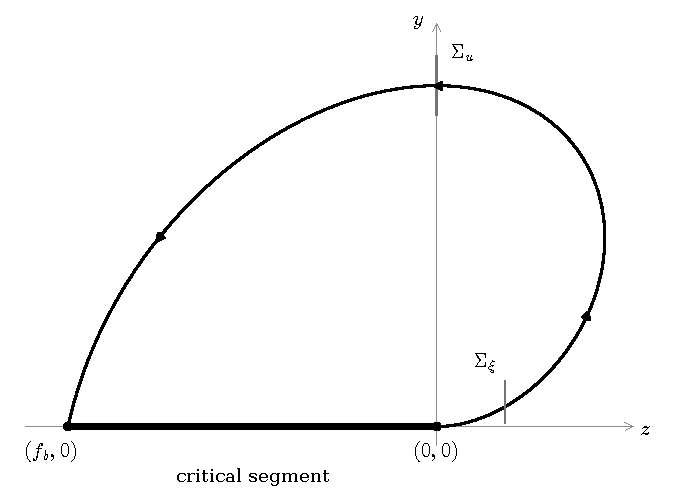
\includegraphics[width=.62\textwidth]{figures/df1b-graphic.pdf}
\caption{The graphic $\Gamma_0^b$ for $b=1/2$, plotted from
\eqref{eq:fast-orbit} with equal coordinate scales. The solid curve is
the fast arc; arrows indicate its direction. Every point of the thick
horizontal segment is an equilibrium of the unperturbed quadratic
field. The short vertical lines indicate transverse sections. The
graphic is not a periodic orbit.}
\label{fig:graphic}
\end{figure}


\subsection{Relation with earlier graphic problems}
The Dumortier--Roussarie--Rousseau program reduces the quadratic
limit-cycle problem to local cyclicity problems for a finite
classification of graphics \cite{DRR1994}. Theorem~\ref{thm:main} gives the sharp count for
cycles converging to this entire graphic. This is the Hausdorff notion
used in the actual counting
statements of \cite[Theorem~3.1]{DR2009} and
\cite[Theorems~1.1--1.2]{Huzak2018}.
The analytic affine and time normalization of
\cite[Proposition~2.1]{DR2009} identifies a neighborhood in the full
twelve-dimensional quadratic coefficient space with this family and
the coordinate and time changes. Using that known normalization,
Corollary~\ref{cor:quadratic-space} transfers the sharp whole-graphic
count to the full coefficient space: the total actual multiplicity is
at most two, and two simultaneous whole-graphic orbits realize the
bound. Corollary~\ref{cor:open-quadratic-realization} further gives
nonempty open sets of coefficients approaching each fixed base field,
with one attracting and one repelling cycle converging to the graphic.
\footnote{The numbering for
\cite{DR2009} refers to the November 30, 2007 author version,
\url{https://www.dms.umontreal.ca/~rousseac/Dumortier_Rousseau.pdf}.}

For normal slow--fast double-saddle cycles,
\cite[Theorem~2.25(ii)]{DMD2008Singular} gives an upper bound two. That result assumes
two persistent hyperbolic corners, a common slow scale with distinct
scaled characteristic ratios, and strict passage conditions between
the corners; Lemma~4.11 there retains the
signed splitting in the connection. Theorem~2.23 of the same paper
also treats certain interior slow saddle-node passages. In the present graphic the
right corner is the turning point itself. As a positive saddle
approaches that point, its characteristic ratio, the physical source
coordinate, and the connection scales degenerate together. Applying
a normal double-saddle comparison in this limit requires uniform
bounds for the complete composed return, including its source
derivatives and signed splitting.

For generic balanced multilayer canards with every side comparison
side-preserving,
\cite[Theorem~4.10, pp.~1346--1347]{DR2008Multilayer} models the actual
rescaled return by translated-power compositions with a controlled
remainder on compact subsets of their positive domain; Corollary~4.11
gives finite cyclicity bounds in that setting. The all-side-preserving
restriction is clarified in \cite{DMD2023SideComparison}.
The separate corrigendum
\cite[p.~1995]{DR2008Corrigendum} gives the smooth functions in equation~(8)
full layer-variable dependence; their single-variable dependence holds
only for their infinite jets at the layer origin.

For ordinary non-transitory canards crossing two open fast layers,
De Maesschalck, Dumortier and Roussarie treat all five connection
diagrams, including side-reversing connections \cite{DMR2025TwoLayer}.
Their Theorem~2 (p.~25), with Definitions~9--10 (p.~24), gives the bound
$\operatorname{Cod}(X)+1$, counting multiplicity, for any unfolding of a
special finite codimensional system $X$.
On its fixed compact layer rectangle, the bound holds for all parameters
in a common neighborhood and all $0<\varepsilon\le\varepsilon_0$, with
no restriction on their relative rates
\cite[proof of Theorem~2, Claim, p.~27]{DMR2025TwoLayer}.
Obtaining an upper bound two from this theorem requires a corresponding
model with $\operatorname{Cod}(X)\le1$.
The original $\Gamma_b$ has only an attracting slow segment and a fast
arc issuing from the contact, so it is not itself an ordinary two-layer
canard. The estimates below follow the signed physical connector
through the degenerating parameter windows, retaining its negative
offset, actual returning domain, and weighted derivatives.

The local contact results of \cite{DMD2010,DMD2011Detectable} provide
finite-order transition and scaled-divergence estimates for finite-order
singular slow dynamics. The global count in
\cite[Theorem~2.7]{DMD2011Detectable} uses normal entry and exit
corners, while Theorems~3.1--3.2 exclude simultaneous zeros of the
slow dynamics at both corners. For the quadratic graphics
$\Gamma_x^b$ whose fast orbit starts at $(x,0)$, the applications in
\cite[Theorem~7]{DMD2010} and
\cite[Theorems~1.1--1.2]{Huzak2018} take $x$ in a compact subset
of $(0,\infty)$. Their source parametrization is regular in that
domain. In the $b=0$ case of \cite{Huzak2018}, for example, the
upper-section height is $1+\sqrt{1+x^2}$, whose derivative vanishes
at $x=0$. We use a regular physical section on the fast arc of
$\Gamma_b$ and estimate the return at this contact endpoint directly.

\enlargethispage{2pt}
Exact smooth normal linearization for specific skew products whose
center dynamics is independent of the normal variables is proved in
\cite[Theorems~1.1 and~1.3, pp.~41--42]{DR2010Normal}; the one-center
result preserves a multiple zero at every parameter value.
Exact finite-smooth normal linearization is also available in
\cite[Theorem~3]{BDMD2011Normal} for a skew product with a fixed
normal spectral gap and sufficiently small center spectrum.\footnote{For \cite{BDMD2011Normal}, this is
Theorem~3, p.~4, of the October 1, 2010 author version; the published
article is cited in the bibliography.}
Our phase and amplitude constructions retain the selected invariant
graph, a common tube with finite phase-derivative bounds, the small
coupling factor in the coordinate shear, and the derivatives after
passage to physical sections
(Lemma~\ref{lem:uniform-normal-product}). These quantitative outputs
are used in the subsequent return comparisons.

\subsection{The counting mechanisms and the proof}
Two coupled degenerations determine the upper proof. At a collision
of slow roots, a through-passage can magnify the incoming height by
an unbounded factor. We retain that factor and cancel it in a weighted
derivative identity. The resulting size and logarithmic-curvature
bounds force one derivative ratio to cross its critical value in one
direction on the actual returning interval
(Lemma~\ref{lem:pc-ratio}). For negative forcing, the preceding slow
segment places every counted return in a common small source interval
before the collision. The through-passage and fiber-exit descriptions
there satisfy the same strict bounds across their finite junction
(Lemma~\ref{lem:pc-event-gluing}). This gives one bound for the field
across the collision.

When both endpoints degenerate, the intermediate map is
$H(a)=\Psi(\eta_0u(a)^R)$, where $\Psi(0)=-B_{\rm conn}<0$.
We retain the complete nonlinear connection. Its negative offset and
small positive derivative give $0<H<u^R$ on the returning interval;
a weighted second-derivative bound controls its contribution to the
return curvature. Source flatness makes the double-saddle comparison uniform both
for a small weak characteristic ratio and as that ratio approaches
one (Lemma~\ref{lem:flat-two-saddle-comparison}). The actual source
interval and the required weighted second-derivative bounds
are verified for this quadratic family. Once each parameter window
controls all counted cycles of one field, a finite cover of the raw
parameter directions gives the common upper bound.

For sharpness, the weak saddle passage is an exact power map with
exponent below one. Its complement is exponentially contracting on
a full signed source rectangle, including the unstable outlet
(Lemma~\ref{lem:realizing-complement}). A small negative splitting
produces a negative--positive--negative displacement on one actual
return interval. Its two zeros give two orbits of the same field;
the image bounds on the rectangle show that each orbit follows the
fast arc and the complete slow segment.

Sections~\ref{sec:return-framework}--\ref{sec:counting} fix the physical
return, normal-product coordinates and scalar comparisons.
Sections~\ref{sec:positive-constant} and~\ref{sec:two-endpoints}
verify the complete collision and connector estimates, and
Section~\ref{sec:parameter-cover} gives their common parameter cover.
The appendices supply the geometric and local passage estimates.
Section~\ref{sec:lower-main} realizes two whole-graphic orbits using
the full complement proved in Appendix~\ref{sec:lower-complement};
Section~\ref{sec:combination} obtains hyperbolicity from the multiplicity
bound. Section~\ref{sec:quadratic-transfer} transfers the result to the
full quadratic coefficient space.
The finite differentiability order in each coordinate argument is
fixed before the parameter windows are shrunk.

\section{The actual return and its multiplicity}\label{sec:return-framework}
A positive function is called a positive unit when it and its reciprocal
are bounded. Phase and section derivatives keep the field parameters
fixed unless a parameter derivative is specified.
Fix $J\Subset(0,2)$ and write $u=u_{\rm up}$ for the reserved
physical coordinate on the upper section. On the fast arc choose
\[
 \Sigma_u^b=\{(0,y_b+u):|u|<u_0\},\qquad
 y_b=1+\exp(\pi b/\sqrt{4-b^2}),
\]
and a small outgoing section $\Sigma_\xi$ at the lower intersection
with $z=\xi>0$. The source and target cores are fixed before the
parameters are shrunk. Let $T_-$ be the backward regular fast transition
and $T_+$ the forward transition through descent, the slow segment,
and contact. The displacement
\begin{equation}\label{eq:common-displacement}
 \Delta(u)=T_+(u)-T_-(u)
\end{equation}
is defined only where both passages exist in finite time.
The target uses the fast first integral $E_b$ of
Lemma~\ref{lem:fast-energy}. In these orientations
$T_-'=-j$, with $j$ and its logarithmic derivatives bounded on the
fixed regular core.

Lemma~\ref{lem:sections} proves that every whole-graphic cycle lies in
$y>0$ and meets each prescribed regular section exactly once.
One Hausdorff inclusion places the orbit near every graphic marker,
forcing a crossing inside the prescribed core; the other confines all
crossings to that core. Jordan separation and the fixed transverse sign
then give uniqueness. The regular holonomies are defined for all initial
values in a smaller core, independently of periodicity.


\subsection{Pullback to actual minimal-return multiplicity}
For two physical sections of the same finite orbit, regular
holonomy $h$ gives $P_2=h\circ P_1\circ h^{-1}$.
Near a return zero,
\[
 h(P_1(s))-h(s)
 =(P_1(s)-s)\int_0^1h'(s+t(P_1(s)-s))\,dt .
\]
The last factor is nonzero at the zero.
A signed energy target or a scaled section change has the same
property on its actual finite-flow domain.
Uniform invertibility at a singular parameter limit is unnecessary;
fixed-field nonzero derivatives suffice.
The regional estimates detect simple zeros or stationary zeros with
nonzero second derivative. Their finite-order section coordinates
therefore determine the order of the physical analytic return zero.

Equilibria and infinite saddle passages bound the actual domain.
At a finite event, two passage formulas describe the same flow at one
source value. Each simple displacement zero has actual multiplicity one,
and each stationary zero with nonzero second derivative has multiplicity two.

\subsection{Normalized coefficient directions}
For each $\mu\ne0$ define $\varepsilon>0$ by
\begin{equation}\label{eq:weighted-radius-main}
 \frac{\mu_1^2+\mu_2^2+\mu_3^2}{\varepsilon^4}
                  +\frac{\mu_4^2}{\varepsilon^6}=1 .
\end{equation}
The left side strictly decreases from infinity to zero, so the
radius is unique. Put $E_i=\mu_{i+1}/\varepsilon^2$ and
$D=\mu_4/\varepsilon^3$. This is a re-expression of the same field;
it does not alter phase coordinates or time. Its direction belongs
to $S^3$, and $\varepsilon(\mu)\to0$ as $\mu\to0$.

Write, exactly,
\begin{equation}\label{eq:upper-normalized}
 F=y(1+bz-y)+\varepsilon^2P(z),\qquad
 G=zy+\varepsilon^3D,\qquad
 P(z)=E_0+E_1z+E_2z^2 .
\end{equation}
All regional estimates below hold on open coefficient windows with
fixed finite phase order, fixed section cores, and one whole-graphic
phase neighborhood.


\section{A common normal-product coordinate}\label{sec:normal-product}

At a simple saddle, a slow-root collision and the lower endpoint, we
start from a selected invariant graph with a fixed normal spectral gap.
The construction below separates the base and normal equations while
preserving that graph. It gives a common tube, uniform finite phase
derivatives, and the small coupling factor needed when passing to
physical sections. Each application first constructs its selected graph.

The persistence result of
\cite[Theorem~3, p.~215]{Fenichel1971} assumes a $C^r$ field,
a compact connected properly embedded $C^r$ invariant manifold,
a hyperbolic splitting, and the source rate inequalities
$\sigma^\pm(m)<1/r$ for every point of that manifold.
We apply it to compact boundaryless extensions after establishing a
fixed normal gap and finite-order rate domination. Its direct conclusion
is invariant-manifold existence. Selection by the tail or incoming
separatrix, the sharp forcing factor, uniform phase jets, and physical
passage are adaptations proved in Sections~\ref{sec:simple-contact-tools},
\ref{sec:positive-constant}, \ref{sec:two-endpoints}, and
\ref{sec:lower-complement}.

\begin{lemma}\label{lem:uniform-normal-product}
Fix an integer $j\ge4$ and nested compact intervals
$I_0\Subset I_1\Subset I_2$. Suppose a chosen invariant graph has been
translated to $u=0$ and the equations are
\begin{equation}\label{eq:uniform-normal-input}
 \dot x=\tau v(x)+\rho c(x,u)u,\qquad
 \dot u=B(x,u)u,\qquad 0<\tau\le\tau_0,
 \quad 0\le\rho\le1.
\end{equation}
On a fixed tube over $I_2$, suppose $v,c,B$ have common
$C^{2j+6}$ bounds in $(x,u)$ and $B$ has one sign with $|B|\ge a_*>0$.
Then, after decreasing $\tau_0$ and the tube radius, there are exact
$C^j$ coordinates on a common tube over $I_0$ in which
\begin{equation}\label{eq:uniform-normal-product}
 \dot\theta=\tau v(\theta),\qquad
 \dot\eta=b(\theta)\eta,
 \qquad b(\theta)=B(\theta,0).
\end{equation}
The coordinate maps and their inverses have common bounds through order
$j$. They preserve the graph and satisfy
\[
 x=X(\theta,\eta)=\theta+\rho\eta L_1(\theta,\eta),
 \qquad u=\eta+\eta^2L_2(\theta,\eta),
\]
where $L_1,L_2$ have common $C^{j-1}$ bounds.
In particular $X_\eta=O_{C^{j-2}}(\rho)$ and the normal coordinate is
uniformly transverse to the graph. All bounds are for phase derivatives
with the field parameters fixed. Zeros of $v$, including multiple zeros,
are allowed.
\end{lemma}

\begin{proof}
 Put $\bar\tau:=|\tau|$. If $B\ge a_*$, first apply the argument to the
 reversed vector field, replacing $v$ by $-v$ so that its base scale is the
 positive $\bar\tau$. All estimates below use this $\bar\tau$; reversing the
 orientation at the end restores the stated equation with the original
 positive $\tau$. We may therefore assume $B\le-a_*$. Extend the already
 translated equations outside $I_2$ with fixed smooth cutoffs, equal to the
 original coefficients on $I_2$, keeping $u=0$ invariant, $B\le-a_*$, and
 the factor $\tau$ in its base flow. Choose the extension of $B$ by a smooth
 interpolation to a negative constant, and taper $v,c$ smoothly only outside
 $I_2$; no extension of a prescribed boundary condition is being asserted.
 This gives bounded coefficients on the whole base line. A smaller normal
 tube is forward invariant. Write $\varphi_t$ for the complete flow of
 $\dot x=\tau v(x)$ and $(x_t,u_t)$ for the full flow.
The asymptotic phase is the convergent limit
\begin{equation}\label{eq:uniform-phase-limit}
 \theta(x,u)=\lim_{t\to\infty}\varphi_{-t}(x_t)
 =x+\rho\int_0^\infty
 D\varphi_{-t}(x_t)c(x_t,u_t)u_t\,dt.
\end{equation}
Indeed $|u_t|\le |u|e^{-a_*t}$ and
$\|D^k\varphi_{\pm t}\|\le K_k(1+t)^{N_k}e^{K_k\bar\tau t}$.
The required differentiated estimates follow directly from the flow
variations. At first order they have coefficient matrix
\[
 \begin{pmatrix}
 \tau v_x+\rho c_xu&\rho(c+uc_u)\\
 B_xu&B+uB_u
 \end{pmatrix}.
\]
Variation of constants and $\int_0^\infty|u_t|dt\le |u|/a_*$
bound the longitudinal variations by a polynomial times
$e^{K\bar\tau t}$.
Every forcing term in a normal variation contains either $u_t$ or a
lower normal variation. Induction through order $j+3$ consequently
bounds the differentiated integrand in \eqref{eq:uniform-phase-limit}
by
\[
 K_j(1+t)^{N_j}
       e^{-(a_*-K_jd-K_j\bar\tau)t},
\]
where $d$ is the normal tube radius. Choose $K_jd<a_*/4$ and then
$K_j\bar\tau_0<a_*/4$. The integral and these derivatives converge
uniformly. In particular $\theta=x$ on $u=0$,
$\theta-x=\rho u L(x,u)$ with bounded finite derivatives, and
$\theta_x=1+O(d)$. Thus $(\theta,u)$ are uniformly invertible
coordinates. The flow identity in the limit gives
$\dot\theta=\tau v(\theta)$ exactly.

In these coordinates write the second equation as
$\dot u=b(\theta)u+q(\theta,u)u^2$ and put
\begin{equation}\label{eq:uniform-amplitude-limit}
 \eta=\lim_{t\to\infty}u_t
       \exp\left(-\int_0^t b(\varphi_s\theta)ds\right)
 =u\exp\left(\int_0^\infty
                    q(\varphi_t\theta,u_t)u_t\,dt\right).
\end{equation}
The same induction, now with the base equation independent of $u$,
gives an integrable majorant for the required derivatives. The last
expression is $u+O(u^2)$ and has positive normal derivative on the
smaller tube. Shifting the limit in time proves
$\dot\eta=b(\theta)\eta$. The inverse function theorem gives the
asserted common coordinate bounds. The input order $2j+6$ leaves more
than the derivatives lost in division by $u$, these two coordinate
changes, and the section changes below. Reversing time back proves
the assertion for either normal sign.
\end{proof}

A product of order $J$ requires $C^{2J+6}$ coefficients and, when a
coefficient contains one derivative of the selected graph, a
$C^{2J+7}$ graph. Fix these orders before shrinking the parameter window.
The simple-contact and positive-collision applications take $J=j+2$,
with graph order at least $2j+11$ and $C^{2j+10}$ coefficients;
this retains the $C^j$ small shear needed for physical sections and the
full collision output $N$. The lower-endpoint product and the lower
$B$ output take $J=j+1$, with graph order $2j+9$ and
$C^{2j+8}$ coefficients. Only finite phase derivatives with the field
parameters fixed are used.

To use the product for physical transitions, we need two section changes. If
$\rho=\tau$ and $|v(\theta_b)|\ge v_*>0$ at an exterior base, the
change from $\theta=\theta_b$ to $x=\theta_b$ has uniformly bounded
finite derivatives. In fact its hitting equation, divided by $\tau$,
is
\[
 \int_0^T v(\varphi_t\theta_b)dt
       +\eta_T L_1(\varphi_T\theta_b,\eta_T)=0,
 \qquad \eta_T=\eta\exp\int_0^T b(\varphi_t\theta_b)dt.
\]
Its derivative in $T$ is bounded away from zero for small $\eta$;
therefore $T=O(\eta)$ with common derivative bounds. The required
lower bound on $|v|$ is at the exterior base; $v$ may vanish inside the
collision strip.

For $\rho=1$, or after a further uniformly smooth change to physical
coordinates, write $z=X(\theta,\eta)$ and $y=H(\theta,\eta)$.
The scaled variable $\eta=\tau V$ gives uniform section bounds in $V$.
Assume again
$|v(\theta_b)|\ge v_*>0$. Suppose $X_\theta$ is a
positive unit and the normal direction is transverse to the graph,
with $a_l:=H_\eta-h_zX_\eta$ a positive unit at
$(\theta_b,0)$, where $y=h(z)$ is the physical graph. Divide
$X(\varphi_T\theta_b,\eta_T)-X(\theta_b,0)=0$ by $\tau$
after this substitution. The implicit function theorem gives bounded
derivatives in $V$ for $|V|\le d_1$, where $d_1>0$ is fixed and small.
To retain the normal factor, write
$H(\theta,\eta)-h(X(\theta,\eta))=\eta a(\theta,\eta)$ and set
$E_T(V)=\exp\int_0^{T(V)}b(\varphi_t\theta_b)dt$. Exactly,
\[
 \frac{\Phi(\tau V)-h(z_b)}{\tau}
 =V E_T(V)a\bigl(\varphi_{T(V)}\theta_b,\tau V E_T(V)\bigr).
\]
The right side has a common $C^{j-1}$ bound and derivative $a_l$ at zero.
Taylor's formula therefore gives
\begin{equation}\label{eq:uniform-physical-section}
 \Phi(\eta)=h(z_b)+a_l\eta+
       \frac{\eta^2}{\tau}E(\eta/\tau),\qquad
 \|E\|_{C^{j-3}}\le K,
 \quad \frac{|\Phi^{(k)}|}{\Phi'}\le K_k\tau^{1-k}
 \quad(2\le k\le j-1).
\end{equation}
Here $z_b=X(\theta_b,0)$ and $\Phi'$ is a positive unit after
decreasing $d_1$. Thus unscaled section derivatives need not remain
bounded as $\tau\to0$.

Finally, if $v$ has a simple zero $\theta_s$ and
$|v'(\theta_s)|$ is a positive unit, division of time by $|b(\theta)|$
gives $\dot\theta=\tau g(\theta)$ and
$\dot\eta=\operatorname{sgn}(b)\eta$. With
$\beta=g'(\theta_s)$, the coordinate
\[
 \xi=\pm(\theta-\theta_s)
 \exp\int_{\theta_s}^{\theta}
       \left(\frac{\beta}{g(t)}-\frac1{t-\theta_s}\right)dt
\]
with the sign chosen to make the incoming coordinate positive,
has common finite derivatives and satisfies
$\dot\xi=\tau\beta\xi$. The integrand has a removable singularity;
the small factor $\tau$ never enters its denominator. When the normal
direction is expanding and $\beta<0$, the passage from
$\xi=\xi_0$ to $\eta=\eta_0$ is exactly
$D(s)=\xi_0(s/\eta_0)^r$, with $r=-\tau\beta$.
This last scalar linearization is used only at simple roots.

\section{Comparisons for the complete return}\label{sec:return-comparisons}\label{sec:counting}

Three scalar comparisons give the upper bound on the complete actual
returning interval of one fixed field. They compare a simple-contact
passage with its complement, control a derivative ratio through slow-root
collision, and compose two endpoint passages with their signed connector.
The physical domains and estimates needed to apply them are proved in
Sections~\ref{sec:positive-constant} and~\ref{sec:two-endpoints}, and
Appendix~\ref{sec:simple-contact}.

\subsection{A simple-contact passage and its complement}
\label{subsec:simple-comparison-core}
For a simple contact with positive preceding slow speed, the bound two
comes from a derivative comparison of the local passage with its
complement. Near the central saddle-node, let $W$ be the scalar
speed in the orbital product coordinates. The passage from the fixed
incoming section $w=w_0>0$ to $s=s_+$ is
$D(s)=w_0\exp(-\int_s^{s_+}dt/W(t))$; write its increasing
complement as $H(a)$. On a subinterval containing every return zero,
the finite-passage condition and complement estimates give $W(H)>0$ and
\[
 \frac{d}{da}\log\frac{D(H(a))}{a}
   =\frac{Z(a)}{aW(H(a))},\qquad
 Z=aH'-W(H),\qquad
 Z'=H'\left(1-W_s(H)+a\frac{H''}{H'}\right)>0.
\]
The logarithmic displacement therefore has at most one stationary
point, a strict minimum. In the saddle ranges, the corresponding
comparison makes every zero of $(D\circ H)'-1$ a strict downward
crossing. For the weak saddle this follows directly from the exact
power $D(s)=\xi_0(s/\omega_0)^r$, $0<r\leq r_0<1$: at $(D\circ H)'=1$,
\[
 (D\circ H)''=\frac{r-1}{rD(H)}+\frac{H''}{H'}<0,
\]
because the complete complement satisfies $r|H''/H'|=o(1)$.
The finite-ratio Dulac estimates give the same conclusion, including
ratios approaching one. In each case a tangent zero is exactly
quadratic and exhausts the local count two.

In the weak-saddle range, early departures form the upper interval
of the physical source, and their displacement is strictly decreasing.
The late interval has the single-maximum property just proved.
After two simple late zeros, or one quadratic late zero, its displacement
is negative up to the finite threshold; continuity and strict decrease
then exclude a threshold or early zero. Otherwise each interval
contributes at most one simple zero. This gives total multiplicity two
on the whole return domain. The local conjugacy is used only where its
outgoing continuation and inverse are both defined; all late outputs
lie in that common image. Appendix~\ref{sec:simple-contact} proves
these domain statements and the derivative estimates above.

\subsection{A weighted derivative ratio through slow-root collision}
\label{subsec:collision-comparison-core}
Let $q_0$ be the scaled incoming height and $\beta$ the fixed-field
separator height on that cut. On the no-root side, $\beta$ is the trace
of the physical outgoing tail; on the root side it is the trace of the
selected incoming stable or parabolic separator. In both cases the actual
returning domain has source distance $s=q_0-\beta>0$.
The incoming reference $q_c(0)$ controls distortion through
$w_\beta=\beta-q_c(0)$; $\beta$ determines the returning boundary.
Section~\ref{sec:positive-constant} constructs these objects and proves
the incoming and outgoing bounds used in the following comparison.

\begin{lemma}
\label{lem:pc-ratio}
Suppose that on an actual returning interval
$s=q_0-\beta>0$, where $\beta$ is independent of $u_{\rm up}$,
$w_\beta=\beta-q_c(0)>0$, and $w_0=s+w_\beta\le C_0$.
Write $M(s)=\partial_s T_+>0$. Assume that, for some $\delta>0$,
\begin{equation}
\label{eq:pc-outgoing-conditions}
 sM(s)\le\varepsilon^2\delta\quad(s\in I),\qquad
 -s(\log M)_s\ge c_M>0\quad(s\in I\cap(0,s_0]),
\end{equation}
where $I$ is the actual returning interval and $s_0,c_M>0$ are fixed.
Assume also that the incoming transition has
\begin{equation}
\label{eq:pc-entry-slope-for-ratio}
 \begin{aligned}
 s_{u_{\rm up}}&=-\varepsilon^{-2}\lambda(s+w_\beta),\qquad
 0<c_\lambda\le\lambda\le C_\lambda,\quad 0<c_j\le j\le C_j,\\
 |(\log\lambda)_{u_{\rm up}}|&\le L_\lambda\varepsilon^{-2},\qquad
 |(\log j)_{u_{\rm up}}|\le L_j.
 \end{aligned}
\end{equation}
on $I$, where all bounds are fixed. These are the incoming and
short-transition estimates from Lemma~\ref{lem:pc-entry} and
\eqref{eq:short-map}. Fix $0<\varepsilon\le\bar\varepsilon$ and put
$K=L_\lambda+C_\lambda+\bar\varepsilon^2L_j$. Require
\begin{equation}\label{eq:pc-ratio-smallness}
 4C_\lambda\delta\le c_j,\qquad
 \delta\le\frac{c_Mc_j}{4K}.
\end{equation}
If the curvature bound is only available for $s\le s_0$, require also
\begin{equation}\label{eq:pc-ratio-localization}
 \frac{4C_\lambda\delta}{c_j}w_\beta<s_0.
\end{equation}
This last condition may be replaced by
$2C_\lambda\delta C_0/c_j<s_0$; it is unnecessary when the curvature
bound holds throughout $I$. Then the isolated return zeros of $T_+-T_-$
have total actual multiplicity at most two.
\end{lemma}

\begin{proof}
Write $u=u_{\rm up}$ and let $R=M|s_u|/j$. The size and incoming bounds give
\[
 R\le\frac{C_\lambda\delta}{c_j}\frac{s+w_\beta}{s}.
\]
Where $R\ge1/2$, the first condition in \eqref{eq:pc-ratio-smallness}
therefore gives
\begin{equation}\label{eq:pc-ratio-source-bound}
 s\le\frac{2C_\lambda\delta}{c_j-2C_\lambda\delta}w_\beta
   \le\frac{4C_\lambda\delta}{c_j}w_\beta.
\end{equation}
Before absorption the same inequality gives
$s\le2C_\lambda\delta(s+w_\beta)/c_j\le2C_\lambda\delta C_0/c_j$.
Thus either cutoff above places these points in the curvature range.
Its logarithmic derivative is
\[
 (\log R)_u=(\log M)_s s_u+
                 (\log\lambda)_u-\varepsilon^{-2}\lambda-(\log j)_u.
\]
At these points $M|s_u|\ge j/2$, so
$|s_u|/s\ge c_j/(2\varepsilon^2\delta)$. The second condition in
\eqref{eq:pc-ratio-smallness} now yields
\[
 (\log R)_u\ge\frac1{\varepsilon^2}
       \left(\frac{c_Mc_j}{2\delta}-K\right)
       \ge\frac{c_Mc_j}{4\varepsilon^2\delta}>0.
\]
Thus $R_{u_{\rm up}}>0$ wherever $R\ge1/2$.
It crosses one at most once, strictly upward.
Since $(T_+-T_-)_{u_{\rm up}}=j(1-R)$, there is at most one stationary
point, a strict maximum. At a stationary return zero,
$(T_+-T_-)_{u_{\rm up}u_{\rm up}}=-jR_{u_{\rm up}}<0$.
Such a zero is quadratic and cannot coexist with another return zero.
Otherwise there are at most two simple zeros. Section~\ref{sec:return-framework}
transfers these orders to actual minimal-return multiplicity.
\end{proof}

In the collision product coordinate, $\eta_0>0$ is the fixed normal
exit height. Write $A$ and $B$ for the normal amplitudes at the left
and right bases. Lemma~\ref{lem:pc-collision-localization} gives an
open physical returning interval $I_{\rm ret}$ on which $0<A<\eta_0$;
every counted cycle has $A<\eta_0/2$.
On the no-root side $B=m_bA$, where $m_b>1$ is the normal expansion
through the strip, without a uniform upper bound. The through and
fibre-exit pieces are the intersections of the actual source with
$0<A<\eta_0/m_b$ and $\eta_0/m_b<A<\eta_0$, respectively.
They are ordered by increasing source distance $s$, opposite to
$u_{\rm up}$, and have at most one finite common boundary.
On the root side only the fibre-exit piece occurs.
Figure~\ref{fig:collision-passages} depicts this partition.
Lemma~\ref{lem:pc-source-partition} includes empty pieces and the finite boundary.

% Schematic product-coordinate passages, not numerical DF1b trajectories.
% Representative curves solve d eta/d theta = .65 eta in drawing units.
% The half-amplitude tick localizes counted zeros; it is not a passage event.
% Native size: approximately 108 mm wide, with 10 pt labels.
\begin{figure}[H]
\centering
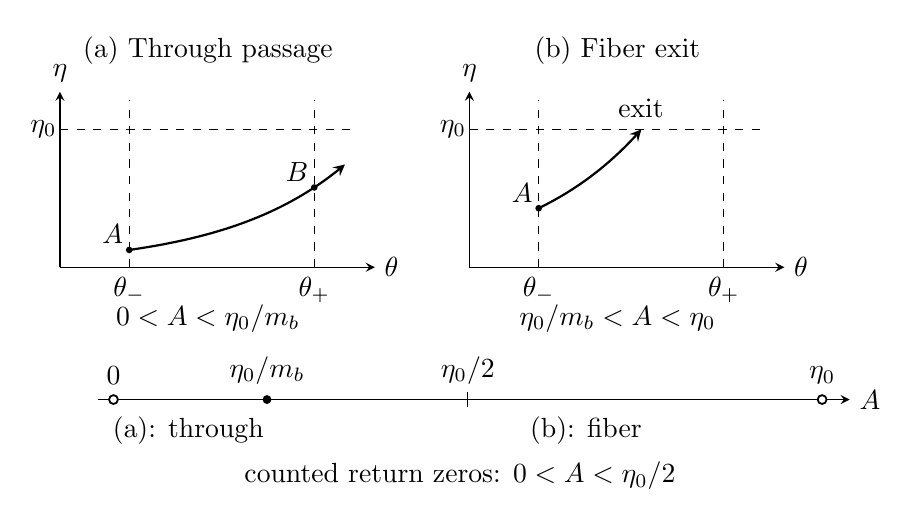
\begin{tikzpicture}[x=10mm,y=10mm,>=stealth,
  every node/.style={font=\fontsize{10}{12}\selectfont},
  axes/.style={->,line width=.45pt},
  section/.style={dashed,line width=.5pt},
  orbit/.style={->,line width=.8pt}]
  \foreach \shift/\panel/\heading in
    {0/a/Through passage,5.2/b/Fiber exit} {
    \begin{scope}[xshift=\shift cm]
      \node at (2,2.75) {(\panel) \heading};
      \draw[axes] (.12,0)--(4.12,0) node[right] {$\theta$};
      \draw[axes] (.12,0)--(.12,2.23) node[above] {$\eta$};
      \draw[section] (1,0)--(1,2.12);
      \draw[section] (3.35,0)--(3.35,2.12);
      \draw[section] (.12,1.75)--(3.83,1.75);
      \node[below] at (1,0) {$\theta_-$};
      \node[below] at (3.35,0) {$\theta_+$};
      \node[left,inner sep=1pt] at (.12,1.75) {$\eta_0$};
    \end{scope}
  }
  \begin{scope}
    \draw[orbit,domain=1:3.74,samples=45,smooth]
      plot (\x,{.22*exp(.65*(\x-1))});
    \fill (1,.22) circle (1.2pt);
    \fill (3.35,{.22*exp(.65*2.35)}) circle (1.2pt);
    \node[above left,inner sep=2pt] at (1,.22) {$A$};
    \node[above left,inner sep=2pt] at (3.35,{.22*exp(.65*2.35)}) {$B$};
    \node at (2,-.65) {$0<A<\eta_0/m_b$};
  \end{scope}
  \begin{scope}[xshift=5.2cm]
    \draw[orbit,domain=1:2.303535169826467,samples=35,smooth]
      plot (\x,{.75*exp(.65*(\x-1))});
    \fill (1,.75) circle (1.2pt);
    \node[above left,inner sep=2pt] at (1,.75) {$A$};
    \node[above,inner sep=2pt] at (2.30,1.82) {exit};
    \node at (2,-.65) {$\eta_0/m_b<A<\eta_0$};
  \end{scope}
  % No-root amplitude order; intersect each branch with the actual image.
  % The filled point is the only possible internal event.
  % The half-amplitude tick and the open outer endpoint are not events.
  \draw[axes] (.6,-1.68)--(10.15,-1.68) node[right] {$A$};
  \draw[fill=white,line width=.65pt] (.8,-1.68) circle (1.6pt);
  \fill (2.75,-1.68) circle (1.6pt);
  \draw[line width=.45pt] (5.3,-1.58)--(5.3,-1.78);
  \draw[fill=white,line width=.65pt] (9.8,-1.68) circle (1.6pt);
  \node[above] at (.8,-1.61) {$0$};
  \node[above] at (2.75,-1.61) {$\eta_0/m_b$};
  \node[above] at (5.3,-1.61) {$\eta_0/2$};
  \node[above] at (9.8,-1.61) {$\eta_0$};
  \node[below] at (1.75,-1.77) {(a): through};
  \node[below] at (6.8,-1.77) {(b): fiber};
  \node at (5.2,-2.65)
    {counted return zeros: $0<A<\eta_0/2$};
\end{tikzpicture}
\caption{Schematic no-root passages in the product coordinates
\eqref{eq:pc-collision-product}. Dashed lines are the fixed bases and exit
level. Trajectory arrows give positive-time direction; the lower line records
increasing $A$. It shows one possible position of the sole seam
$A=\eta_0/m_b$ in $0<A<\eta_0$;
intersect the displayed branch ranges with the actual source image.
Here $m_b>1$ has no uniform upper bound, and the seam or a branch may be
absent from that image. The half-amplitude tick marks localization of
counted return zeros, not a passage event. When a root is present, only
fiber exit remains; $B=m_bA$ is the no-root through relation.}
\label{fig:collision-passages}
\end{figure}


The through and fibre-exit formulas describe one physical passage, so
the derivative comparison must hold across their finite boundary. The
next lemma gives the common constants and cutoff condition needed for
this step. Section~\ref{sec:positive-constant} verifies its flow and
domain hypotheses.

\begin{lemma}[Finite-event gluing for the collision return map]
\label{lem:pc-event-gluing}
Fix one negative-forcing field in the collision coefficient box, and let
$I_{\rm ret}$ be the restricted physical source from
Lemma~\ref{lem:pc-collision-localization}, after the common target-core
restriction. On the no-root side, the through and fibre-exit formulas in
\eqref{eq:pc-source-partition} are restrictions of one flow-defined
$C^2$ map $\widehat T_+$ on $I_{\rm ret}$, with
$M=\partial_s\widehat T_+>0$. Thus $M$ and $M_s$ are continuous at
the possible finite event $A=\eta_0/m_b$.
Assume the incoming and short-transition bounds of
Lemma~\ref{lem:pc-ratio} on $I_{\rm ret}$.
Suppose the estimates \eqref{eq:pc-outgoing-conditions} hold on the
nonempty open pieces, with
constants $(\delta_\ell,c_\ell)$ for
$\ell\in\{\mathrm{through},\mathrm{fibre}\}$. Set
$\delta=\max_\ell\delta_\ell$ and $c_M=\min_\ell c_\ell$.
Require \eqref{eq:pc-ratio-smallness} with the common incoming bounds.
On a row whose curvature bound is restricted to $s\le s_{0,\ell}$,
require in addition
$4C_\lambda\delta_\ell w_\beta/c_j<s_{0,\ell}$, or
$2C_\lambda\delta_\ell C_0/c_j<s_{0,\ell}$.
No such restriction is needed when a row's curvature bound holds
throughout its returning interval.
Then the estimates extend to the finite event, and the complete displacement
$\widehat\Delta=\widehat T_+-T_-$ has total actual isolated zero multiplicity
at most two on $I_{\rm ret}$. On the root side the same conclusion
holds under these estimates for the single fibre-exit piece, with no
internal finite event.
\end{lemma}
\begin{proof}
At the finite event the returning flow has finite flight time, so the
two formulas have the same value and first two derivatives.
Since $s>0$ and $M>0$, continuity of $M$ and $M_s$ extends
$sM$ and $-sM_s/M$ to that value. Where the derivative ratio in
Lemma~\ref{lem:pc-ratio} is at least $1/2$,
\eqref{eq:pc-ratio-source-bound} with $\delta_\ell$, or its $C_0$
alternative, puts the source in the range of the row's curvature bound.
The proof of that lemma
gives the crossing inequality with a common positive margin on both
pieces and, by continuity, at the event. Its single-maximum argument consequently
applies on the whole source interval. On the root side it applies
directly to the single fibre-exit interval.
\end{proof}
\subsection{A two-saddle comparison with a flat source}
\label{subsec:flat-source-comparison}
For simultaneous endpoint degeneration, we compare the positive Dulac
passage with the complete nonlinear connector $H=\Psi(\eta_0u^R)$.
The scalar comparison permits a nonpositive baseline $\Psi(0)\le0$.
For the quadratic family, Proposition~\ref{prop:complete-signed-connector}
constructs the connector on its full signed source interval with a
strictly negative baseline and the required weighted derivative bounds.
Source flatness and second derivatives suffice, including when the
positive characteristic ratio approaches one.

\begin{lemma}[Two-saddle comparison with a flat source]
\label{lem:flat-two-saddle-comparison}
Fix the vector field parameters and let $I\subset(0,\infty)$ be an open
actual returning interval. Let $u\in C^2(I)$ satisfy
\[
 0<u<1,\qquad u'>0,\qquad |u''/u'|\le M.
\]
For fixed $R>1$ and $\eta_0>0$, put
$t=\eta_0u^R$ and $H=\Psi(t)>0$. Assume that
$\Psi\in C^2([0,t_*])$, $t(I)\subset(0,t_*)$, and
\[
 \Psi(0)=-B_{\rm conn}\le0,\qquad \Psi'>0,\qquad
 \eta_0\sup_{[0,t_*]}\Psi'\le1,\qquad
 \left|t\frac{\Psi''(t)}{\Psi'(t)}\right|\le L_\Psi.
\]
Let $\mathcal D\in C^2$ with $\mathcal D'>0$ on a positive interval
containing $H(I)$. All derivatives are taken with the field parameters
fixed. The equation $\mathcal D(H(a))=a$ has total isolated zero
multiplicity at most two on $I$ in either of the following situations:
\begin{enumerate}
 \item $\mathcal D(s)=c_Ds^r$, $0<c_D\le C_D$,
       $0<r\le r_0<1$, $Rr\ge1$, $0<\mathcal D(H)\le a_0$, and
       $Rr\sup_Iu'\le\eta_*$. The bounds $C_D,r_0,M,L_\Psi$ are fixed,
       and $a_0,\eta_*>0$ are sufficiently small in terms of them;
 \item $r\in[r_*,r^*]\Subset(0,\infty)$, $Rr\ge1+\kappa$ for a fixed
       $\kappa>0$,
       $0<H'\le m$, $R\sup_Iu'\le M_f$, and
       \begin{equation}\label{eq:lower-dulac-jets}
        0<\mathcal D'\le M_Ds^{r-1},\qquad
        \frac{s\mathcal D''}{\mathcal D'}=r-1+E(s),\qquad
        |E|\le M_Ds^\alpha,
       \end{equation}
       on the positive domain of $\mathcal D$. Here
       $\alpha,M_D,M_f>0$ and $r_*,r^*,M,L_\Psi$ are fixed,
       $E$ is continuous, and $m>0$ is sufficiently small in terms of
       these bounds and $\kappa$.
\end{enumerate}
Every stationary zero has nonzero negative second derivative.
In the second case the conclusion is uniform as $r$ approaches one,
and if $r\ge1$ there is at most one zero, which is simple.
\end{lemma}

\begin{proof}
The signed-connector hypotheses give
\[
 0<H\le\Psi(t)+B_{\rm conn}
      =\int_0^t\Psi'(v)\,dv\le u^R<1.
\]
Put $v=(\mathcal D\circ H)'$, $U=u''/u'$,
$W(s)=s\mathcal D'(s)$, $\sigma(s)=s\mathcal D''(s)/\mathcal D'(s)$,
and $\Lambda(t)=t\Psi''(t)/\Psi'(t)$. Direct differentiation gives
\begin{equation}\label{eq:lower-critical-barrier}
 \begin{aligned}
 \frac{H''}{H'}&=[R-1+R\Lambda(t)]\frac{u'}u+U,\\
 v'&=\frac{H'}H J\quad\hbox{at }v=1,
 \end{aligned}
\end{equation}
where
\[
 J=\sigma(H)+W(H)U+
        W(H)[R-1+R\Lambda(t)]\frac{u'}u.
\]
We prove $J<0$ at every such point. Set $C_\Psi=1+L_\Psi$.
In the first case $W(H)=r\mathcal D(H)$ and $\sigma=r-1$.
Since $u^{Rr-1}\le1$, including when $Rr=1$,
\[
 R W(H)\frac{u'}u
 \le C_D Rr u'u^{Rr-1}\le C_D\eta_*.
\]
Take $a_0$ first, then $\eta_*$, so that
$r_0Ma_0+C_\Psi C_D\eta_*\le(1-r_0)/2$. Consequently
\[
 J\le-(1-r_0)+r_0Ma_0+C_\Psi C_D\eta_*
   \le-(1-r_0)/2<0.
\]

In the second case $r\ge1$ gives $v\le M_DmH^{r-1}\le M_Dm<1$
once $M_Dm<1$, so only $r<1$ needs consideration.
Write $\beta=1-r$ and $T=\log(1/H)$.
At $v=1$, the bound on $\mathcal D'$ implies
\[
 \beta T\ge L_m:=\log\frac1{M_Dm}.
\]
Since $Rr\ge1+\kappa$, put
$\gamma_\kappa=r_*\kappa/(1+\kappa)>0$. Then
\[
 r-\frac1R\ge\frac{r\kappa}{1+\kappa}\ge\gamma_\kappa.
\]
Using $u\ge H^{1/R}$ gives
\[
 R W(H)\frac{u'}u\le M_D M_f H^{r-1/R}
                  \le M_D M_f H^{\gamma_\kappa}.
\]
It follows that
\[
 J\le-\beta+M_DH^\alpha+M_DM H^{r_*}
                      +C_\Psi M_DM_f H^{\gamma_\kappa}.
\]
Put $\zeta_\kappa=\min\{\alpha,\gamma_\kappa\}>0$ and
$C=M_D(1+M+C_\Psi M_f)$. Choose
\[
 0<m\le\frac1{M_D}
       \exp\left(-\frac{\max\{1,\log(4C)\}}{\zeta_\kappa}\right).
\]
Then $M_Dm<1$, $L_m\ge1/\zeta_\kappa$ and
$Ce^{-\zeta_\kappa L_m}\le1/4$.
At the critical points $T\ge L_m$, since $0<\beta<1$, and hence
\[
 \frac{H^{\zeta_\kappa}}{\beta}
 \le\frac{T e^{-\zeta_\kappa T}}{L_m}
 \le e^{-\zeta_\kappa L_m}.
\]
Thus $J\le-3\beta/4<0$ with one choice of $m$ depending on $\kappa$,
uniformly as $r\to1$.

Every zero of $v-1$ is a strict downward crossing by
\eqref{eq:lower-critical-barrier}. There is at most one: two downward
crossings would require an intervening upward or nontransverse crossing.
The displacement is therefore strictly monotone, or increases before
its unique critical point and decreases afterward. It has at most two
simple zeros or a single quadratic zero with negative second derivative;
a zero interval is impossible. Section~\ref{sec:return-framework}
transfers these orders to actual minimal-return multiplicity.
\end{proof}


\section{Positive contact constant and slow-root collision}
\label{sec:positive-constant}

The remaining contact scaling has two independent small parameters:
\begin{equation}
\label{eq:pc-family}
 F=y(1+bz-y)+\varepsilon^2P(z),\qquad
 G=zy+\kappa^3d,\qquad
 P(z)=z^2+arz+r^2,\qquad \kappa=r\varepsilon.
\end{equation}
Throughout this section, $a,d$ range in fixed compact intervals and
$r,\varepsilon>0$ tend to zero independently. In particular, estimates
must allow $r$ to be smaller than every power of $\varepsilon$.

\begin{proposition}
\label{prop:positive-constant}
On every compact $(a,d,b)$-set with $0<b<2$, all sufficiently small
fields \eqref{eq:pc-family} have total actual minimal-return multiplicity
at most two for isolated cycles in one Hausdorff neighborhood of the
whole limiting graphic. The parameter
and Hausdorff neighborhoods are uniform on that compact set.
For $d\ge0$ the bound is one and every counted zero is simple.
\end{proposition}

Near a positive double root, the slow passage can amplify the incoming
height by an arbitrarily large factor. We retain this multiplier in
product coordinates. Weighting the complete outgoing derivative by the
incoming distance from the separating trajectory cancels the multiplier
and gives size and logarithmic-curvature bounds. Combined with the
incoming distortion estimate, these bounds force the derivative ratio
with the short map to cross one only upwards
(Lemma~\ref{lem:pc-ratio}).

Lemma~\ref{lem:pc-entry} controls the incoming trace, and
Lemma~\ref{lem:pc-normal-derivative} estimates the logarithmic derivative
from departure to the target. Before applying the comparison at a
collision, Lemma~\ref{lem:pc-collision-localization} places every counted
cycle in one small source interval. Lemma~\ref{lem:pc-source-partition}
divides it into through passages and fiber exits; on the root side only
the fiber exit occurs (Figure~\ref{fig:collision-passages}). At their
possible finite junction, the two formulas represent the same physical
return. Lemma~\ref{lem:pc-event-gluing} therefore gives the bound two on
the whole interval.

\subsection{The incoming map in a regular coordinate}

We first transport the upper-section source to the inner cut $z=0$.
The signed variation of its height will control the derivative of the
complete contact map.

Use the signed coordinate $u_{\rm up}$ on the upper section from
Lemma~\ref{lem:sections}. Every counted cycle meets this section exactly
once.
The same lemma supplies the contact passage in $y>0$, $F>0$,
from the decreasing-height section $y=K\varepsilon^3$ to a fixed
positive section, on the interval of sources for which that passage is
defined. No sign or scaled-size condition is imposed on $u_{\rm up}$.
Set
\begin{equation}
\label{eq:pc-inner}
 z=\kappa\zeta,\quad y=\kappa^2q,\quad
 q_0(u_{\rm up})=q(0;u_{\rm up}),\qquad
 q_\zeta=\frac{\zeta q+d}{V(\zeta,q)},\quad
 V=\mathsf A+\mathsf Bq-\mathsf Cq^2,
\end{equation}
where
\[
 \mathsf A=1+a\varepsilon\zeta+\varepsilon^2\zeta^2,
 \qquad \mathsf B=1+b\kappa\zeta,\qquad \mathsf C=\kappa^2.
\]
All derivatives below keep the vector field fixed.

\begin{lemma}
\label{lem:pc-entry}
The actual incoming values satisfy $0<q_0\le Q_0$, with $Q_0$
uniform. There is a particular solution $q_c$, independent of
$u_{\rm up}$, such
that $q_0=q_c(0)+w_0$, $w_0>0$. For $d\ge0$,
\begin{equation}
\label{eq:pc-entry-positive}
 q_c(0)\ge0,\qquad
 \frac{|(q_0)_{u_{\rm up}}|}{q_0+d}\le C\varepsilon^{-2}.
\end{equation}
For $d=-m<0$, a cycle is possible only if
\begin{equation}
\label{eq:pc-exponential-wedge}
 a<0,\qquad 0<m\le C\exp(-c/\varepsilon^2).
\end{equation}
On this set $-4m\le q_c(0)<0$ and
\begin{equation}
\label{eq:pc-entry-negative}
 (\log w_0)_{u_{\rm up}}=-\varepsilon^{-2}\lambda,
 \qquad c\le\lambda\le C,\qquad
 |(\log\lambda)_{u_{\rm up}}|\le C\varepsilon^{-2}.
\end{equation}
The passing and target restrictions have interval preimages in
$u_{\rm up}$.
\end{lemma}

\begin{proof}
We first justify the full incoming passage. On a fixed negative interval,
$P(z)\ge z^2/2$ for small $r$. Put $x=-z$ and subtract the forcing
graph $\kappa^3d/x$. For $x\ge Mr$, with $M$ fixed and large, the
two sides of
\[
 \left|y-\frac{\kappa^3d}{x}\right|
       \le k\varepsilon^2x^2
\]
point inward; this follows by substituting the two equalities in
$dy/dz=G/F$, using $P\asymp x^2$ and then choosing $M$ large.
It carries the fixed negative entrance to $Z=z/r=-M$, with bounded
small normal coordinate in
\[
 Y=\frac{y}{r^2\varepsilon^2},\qquad
 w=Y+\frac{\varepsilon d}{Z}.
\]
On a fixed negative $Z$-interval the normal eigenvalue is bounded away
from zero. The invariant graph and strong foliation give an exact
scalar base equation $\dot\theta=\varepsilon^2UQ_\varepsilon(\theta)$,
where $U>0$ and, before the near-identity base change,
\[
 Q_\varepsilon(Z)=Z^2+aZ+1-\frac{\varepsilon d(1+brZ)}Z
                         -\frac{r^2\varepsilon^4d^2}{Z^2}.
\]
Its second derivative is positive on this fixed strip for sufficiently
small parameters, so it has at most two roots. The normal coordinate
contracts at a fixed rate.
The base at entry lies in $(-M-1/2,-M+1/2)$; choosing $M$ larger puts
this entire interval to the left of every possible negative root.
A first root cannot be crossed by the scalar base. Its approach takes
infinite time and normal contraction makes this alternative terminal.
If there is no root, the exit at a fixed $Z=-\zeta_0<0$ satisfies
\[
 |w|\le C\varepsilon^3+C e^{-c/\varepsilon^2}.
\]
The two sides of $|q+d/\zeta|\le K/\zeta^2$ point inward on
$-\zeta_0/\varepsilon\le\zeta\le-L$, and $V$ lies between two
positive constants there. This gives a bounded entrance at $\zeta=-L$.
These assertions use the strong spectral gap, not a lower bound for a
weak root derivative. The fixed-gap graph transform, as in the proof
of Lemma~\ref{lem:small-ratio-saddle}, first supplies the invariant
graph and its finite phase bounds on this negative strip.
Lemma~\ref{lem:uniform-normal-product} then applies with
$\tau=\rho=\varepsilon^2$ and negative normal sign. No scalar base
linearization is made, so its conclusion includes a negative double
root as well.

Here is a direct bound on the last inner ordinate. In $X=z/r$ and
$Y=y/(r^2\varepsilon^2)$ the equations are
\[
 X'=\varepsilon^2(YQ+p_a(X)),\quad
 Y'=XY+\varepsilon d,\quad
 Q=1+brX-r^2\varepsilon^2Y,\quad p_a=X^2+aX+1.
\]
The preceding upper barrier gives $Y(-L_1)\le K_1$ for a fixed large
$L_1$. Choose $T>K_1+4\max_{[-L_1,0]}|p_a|+1$. Above $Y=T$,
$YQ+p_a\ge Y/4$. If $d\le0$, $Y$ decreases for $X<0$. If $d>0$,
an upcrossing of $Y=T$ requires $X\ge-\varepsilon d/T$; thereafter
\[
 \frac{d(Y^2)}{dX}\le\frac{8d}{\varepsilon}.
\]
The remaining interval has length at most $\varepsilon d/T$.
Thus $Y(0)^2\le T^2+8d^2/T$. This proves the uniform bound on $q_0$.

Select the particular solution $y_c$ by zero strong amplitude on the
incoming invariant graph and continue the same solution through the
taper and the inner funnel. The strong-graph equation gives, on every
fixed negative interval,
\[
 y_c=-\kappa^3d/z+O(\varepsilon^2\kappa^3|d|),
 \qquad \partial_z^jy_c=O(\kappa^3|d|),\quad j\le2.
\]
The construction is made on the nested negative intervals with the
same graph, so these are restrictions of one solution. For $d=0$ it
is exactly zero. For $d\ne0$ its sign on the incoming half is the
sign of $d$: at $y=0$ the scalar velocity has that sign, and the
selected forced trace cannot cross to the other side. Its continuation
to $z=0$ has the same sign. At the decreasing-height entrance
$z=\Lambda(u_{\rm up})$,
\[
 W_i:=K\varepsilon^3-y_c(\Lambda)\asymp\varepsilon^3>0.
\]
Scalar uniqueness preserves $W=y-y_c>0$ along every passing interval.

For the needed variational estimates write, exactly,
\begin{equation}
\label{eq:pc-tail-feedback}
 \begin{aligned}
 W_z&=A(z,W)W,&
 A(z,W)&=\int_0^1H_y(z,y_c+tW)\,dt,\\
 L_z&=WA_WL,& L&=(\log W)_{u_{\rm up}},\qquad H=G/F.
 \end{aligned}
\end{equation}
Because the entrance moves, its fixed-phase initial value is
\begin{equation}
\label{eq:pc-moving-entry}
 L_i=\frac{(W_i)_{u_{\rm up}}}{W_i}
       -A(\Lambda,W_i)\Lambda_{u_{\rm up}}.
\end{equation}
The moving entry satisfies the common $C^2$ estimate
\eqref{eq:relaxation-map}, proved by integrating
\eqref{eq:relaxation-error}; its error from the fast-foot map is
$O(\varepsilon^2(1+|\log\varepsilon|))$.
At this section
\[
 A(\Lambda,W_i)
 =\frac{\Lambda}{\varepsilon^2P(\Lambda)}(1+O(\varepsilon)).
\]
It follows that $|L_i|\le C\varepsilon^{-2}$ and, for negative $d$,
$L_i=-\varepsilon^{-2}\lambda_i$, where $\lambda_i$ is a positive
unit with bounded logarithmic $u_{\rm up}$-derivative.

To propagate the initial variation through the shrinking scales, we
bound the feedback integrals. On the fixed negative interval,
\[
 |H_{yy}|\le C\varepsilon^{-4},\quad
 |H_{yyy}|\le C\varepsilon^{-6},\quad
 W\le C\varepsilon^3e^{-c(z-\Lambda)/\varepsilon^2}.
\]
On the taper from $x_g$ to $Mr$,
\[
 \begin{gathered}
 |H_{yy}|\le C\varepsilon^{-4}x^{-3},\qquad
 |H_{yyy}|\le C\varepsilon^{-6}x^{-5},\\
 W(-x)\le W_g(x/x_g)^N,\qquad N=c/\varepsilon^2,\qquad
 W_g\le C\varepsilon^3e^{-c/\varepsilon^2}.
 \end{gathered}
\]
Integrating these powers down to zero bounds the first feedback by
$CW_g/(\varepsilon^2x_g^2)$ and the second by
$CW_g^2/(\varepsilon^4x_g^4)$. On a passing negative root interval,
the exact strong equation $\dot\eta=-b_n(\theta)\eta$,
$b_n\ge c>0$, bounds the first feedback by
$C\int|\eta(0)|e^{-ct}\,dt$. The endpoint changes
$Z=\theta+O(\varepsilon^2\eta)$ have the same bound. To control a
fixed physical section without dividing by a small base speed, write
$\dot\theta=\varepsilon^2v(\theta)$ on a passing branch, where $v>0$.
The entrance speed is a positive unit, $v'$ is bounded, and
\[
 \frac d{dt}\log\frac{|\eta|}{v}
       =-b_n-\varepsilon^2v'\le-c/2.
\]
Consequently $|\eta|/v\le C|\eta(0)|e^{-ct/2}$, which controls
the ratio occurring in the physical-section correction. Indeed, the
product inverse has $Z=\theta+\varepsilon^2\eta L_1$ and
$u=\eta+\eta^2L_2$, with bounded finite jets. Thus $v(Z)$ is
comparable with $v(\theta)$ and the physical speed
$v(Z)+c(Z,u)u$ is a positive unit times $v(Z)$, provided the entrance
amplitude is fixed sufficiently small. For the divided physical
coefficient $a=B/[\varepsilon^2(v+cu)]$, direct differentiation gives
\[
 |u a_u|\,dZ\le C\left(|u|+\frac{|u|}{v(Z)}\right)dt,
 \quad
 |u^2a_{uu}|\,dZ\le C\left(u^2+\frac{u^2}{v(Z)}
                                      +\frac{u^2}{v(Z)^2}\right)dt.
\]
The preceding decay bounds make both integrals finite with a common
bound. The physical feedback equations are differentiated at fixed
$Z$; the product coordinates are only used to estimate their
coefficients. Weak flight time need not be bounded; a base root
reached only at infinite time is terminal and is excluded from this
passing branch.
For negative $d$, the restriction $a<0$ proved below gives
$p_a(Z)\ge1+Z^2$ for $Z<0$. On the fixed negative scaled interval the
scalar equation then has $A\le-c/\varepsilon^2$ and its first two normal
derivatives are $O(\varepsilon^{-2})$, which also bounds the second
feedback.

For $d=-m<0$, a bound proportional to $m$ will localize the later ratio
estimate. At a fixed small negative contact point $z=-x_*$, the selected
incoming graph has
$q_c(-x_*/\kappa)=-\kappa m/x_*+O(\varepsilon^2\kappa m)$.
On the interval from that point to zero, $a<0$ gives $\mathsf A\ge1$.
The graphs $-4m/(1-\zeta)$ and zero are lower and upper barriers.
Indeed, writing $t=-\zeta$, at the lower graph the numerator
$\zeta q-m$ is nonnegative for $t\ge1/3$. For $0\le t\le1/3$,
$V\ge1/2$ bounds the scalar right-hand side below by $-2m$, while the
lower graph has derivative at most $-9m/4$. The initial value is between
the two barriers;
at the upper graph that right-hand side is $-m/\mathsf A<0$. Thus
$-4m\le q_c(0)<0$, with no reciprocal small scale or root gap.

In the funnel set $q=q_c+w$. Its exact divided coefficient is
\[
 a_f=\frac{\mathsf N}{V(\zeta,q_c)V(\zeta,q_c+w)},\quad
 \mathsf N=\zeta\mathsf A-d\mathsf B+
 \mathsf C\{\zeta q_c^2+2dq_c+w(\zeta q_c+d)\}.
\]
On the funnel ending at $\zeta=-L$, with $L$ fixed and large,
$\mathsf N\le-c(|\zeta|+d)$ for $d\ge0$; in the negative
exponential range it is at most $-c|\zeta|$. The speeds are positive
units, and $B_f=(a_f)_w/a_f$ and $(B_f)_w$ are bounded. Since
$w_\zeta=a_fw<0$ and $(a_f)_{ww}=a_f(B_f^2+(B_f)_w)$, the feedback
integrals are bounded by $C\int(-w_\zeta)d\zeta$. The remaining
bounded inner interval $[-L,0]$ has bounded third height derivatives;
the sign of $a_f$ need not stay negative there.
Consequently
\begin{equation}
\label{eq:pc-feedback-mass}
 \int|WA_W|\,dz\le C,\qquad
 \int(|WA_W|+|W^2A_{WW}|)\,dz\le C\quad(d<0).
\end{equation}
Linear changes of phase leave these integrals unchanged. The strong
coordinate calculation above includes the endpoint terms when that
coordinate is used in the negative root interval.

Equations \eqref{eq:pc-tail-feedback}--\eqref{eq:pc-feedback-mass}
preserve $|L|\le C\varepsilon^{-2}$. For $d\ge0$,
$q_0+d\ge w_0$ proves \eqref{eq:pc-entry-positive}. For $d<0$ write
$L(0)=L_i e^{J(u_{\rm up})}$,
$J=\int_{\Lambda(u_{\rm up})}^0WA_W\,dz$. Then
\[
 J_{u_{\rm up}}=-[WA_W]_{\Lambda}\Lambda_{u_{\rm up}}+
              \int L(WA_W+W^2A_{WW})\,dz=O(\varepsilon^{-2}).
\]
The first term is $O(\varepsilon^{-1})$; the second is controlled by
\eqref{eq:pc-feedback-mass}. This proves
\eqref{eq:pc-entry-negative}.

It remains to justify the restriction used on negative $d$.
Lemma~\ref{lem:damping} excludes $a\ge0$. For $d=-m<0$ and $x\ge L_1r$,
the upper barrier and $F\le C\varepsilon^2x^2$ give
\[
 y(-L_1r)\le K\varepsilon^3
       (L_1r/x_g)^{c/\varepsilon^2}.
\]
The height decreases to $z=-\kappa$. Division by $\kappa^2$ loses
only $r^{-2}$: for $N>2$, $r^{-2}(L_1r/x_g)^N$ is increasing in
$r$. Choosing $r_0<x_g/(2L_1)$ gives $q(-1)\le Ce^{-c/\varepsilon^2}$,
uniformly even for arbitrarily small $r$. On $-1\le\zeta\le0$,
$q_\zeta\le-m/2$ as long as $q>0$. Positivity at zero proves
\eqref{eq:pc-exponential-wedge}. Finally, scalar order, $F_y>0$,
and the fixed target interval show that every intervening solution
between two retained ones is retained. Thus the restrictions are
intervals.
\end{proof}

Let $T_-(u_{\rm up})$ be the short map in the energy coordinate $E_b$,
and $T_+(u_{\rm up})$ the map obtained by the contact passage and outgoing arc.
Lemma~\ref{lem:sections} gives
\begin{equation}
\label{eq:pc-short}
 (T_-)_{u_{\rm up}}=-j(u_{\rm up}),\qquad c\le j\le C,\qquad
 |(\log j)_{u_{\rm up}}|\le C.
\end{equation}
Their intersections correspond to captured periodic orbits; their isolated
intersections are precisely the limit cycles being counted.

\paragraph{Actual-domain scope on the nonnegative side.}
For $a>0$ the negative scaled strip may have a base root. The incoming
product in Lemma~\ref{lem:pc-entry} then cannot pass its first root:
its base approaches only in infinite time while the normal deviation
contracts. Such a field has no retained passage to $z=0$, also at
$d=0$. On a no-root branch that lemma controls feedback on the whole
returning interval.
The outgoing and short-map constants can be fixed on fixed
enlarged physical cores before shrinking $\xi$; regular energy
holonomy has a uniform unit bound there. After these constants
are fixed choose $\xi$, then $r$, and finally $\varepsilon$.

\subsection{Nonnegative forcing and a comparison criterion}

For nonnegative forcing, a weighted variational identity makes the
complete contact derivative smaller than the short-map derivative.

For $d\ge0$, the required outgoing estimate holds even when $P$ has
positive roots. Let $J=\partial_{q_0}q$ in \eqref{eq:pc-inner} and
$h=q_0+d>0$. On $0\le\zeta\le1$, direct integration gives
$q(1)\ge ch$ and $0<J(1)\le C$. For $\zeta\ge1$ put
\[
 \mathcal R=hJ\frac{V(\zeta,q)}q.
\]
The exact cancellation
\begin{equation}
\label{eq:pc-positive-cancellation}
 (\log\mathcal R)'=\frac{(V_\zeta)|_q-d/q}{V}
\end{equation}
is obtained by differentiating the scalar and variational equations.
The function $\Phi=\mathsf Bq-\mathsf Cq^2$ increases, since
$q'\ge0$ and $\mathsf B-2\mathsf Cq=F_y>0$. The integral of
$\mathsf B'q/V$ is bounded: outside a negative well of $\mathsf A$,
or when $q$ is large, $q/V\le C$; on the remaining bounded-height
part use
\[
 \frac{\mathsf B'q}{V}\,d\zeta
 =\frac{\mathsf B'q}{\zeta q+d}\,dq
 \le\frac{\mathsf B'}\zeta\,dq.
\]
There $\zeta\ge c/\varepsilon$. To integrate
$\mathsf A'/(\mathsf A+\Phi)$, pair the decreasing and increasing
branches of the convex quadratic at equal values of $\mathsf A$.
The later denominator is larger, so each paired contribution is
nonpositive, including when $\mathsf A\le0$. Only a final increase
above $\mathsf A(1)>c$ remains. At a fixed section $z=\xi$ this gives
\[
 \mathcal R_{\rm out}\le C(1+\xi^2/r^2),\qquad
 (q_0+d)\partial_{q_0}T_+
          \le C(\kappa^2+\varepsilon^2\xi^2).
\]
The factor $\kappa^2$ converts $q$ to the physical ordinate. The
regular continuation in the $E_b$ coordinate has derivative tending
to one after $\xi$ is fixed. With \eqref{eq:pc-entry-positive},
\[
 |(T_+)_{u_{\rm up}}|\le C(r^2+\xi^2).
\]
Choose $\xi$ small and then $r$ small so that the last bound is less
than $j/2$. The displacement is strictly increasing and has at most one
zero, necessarily simple, on its returning interval.

For negative $d$, we use Lemma~\ref{lem:pc-ratio} after identifying
the physical separator and estimating the departure map.

\subsection{Changing the incoming reference preserves the physical separator}
Write $d=-m<0$ and $u=u_{\rm up}$. Lemma~\ref{lem:pc-entry}
has already placed every counted cycle in the wedge $a<0$ with $m$
exponentially small. To estimate incoming distortion, we may replace
the selected incoming reference $y_c^o$ by the solution $y_c^n$ whose
value at a fixed negative point is zero. The outgoing separator is
still the trace $\beta=y_\sigma(0)/\kappa^2$, with source distance
$s=q_0-\beta>0$. We verify that this change of reference preserves
the complete derivative comparison.

Both incoming solutions obey the barriers
$-4m/(1-\zeta)\le q_c^i(\zeta)<0$, $i=o,n$, on their
common terminal negative interval. For $\zeta\in[-1/8,0]$,
$1\le\mathsf A\le2$, $\mathsf B>0$, and
$1/2\le V(\zeta,q_c^i)\le2$ after shrinking.
Moreover $\zeta q_c^i\le m/2$. Their exact scalar equations
therefore give $(q_c^i)_\zeta\le-m/4$, hence
\[
 -4m\le c_i:=q_c^i(0)\le-m/32 .
\]
The old incoming graph's initial value lies between these same
barriers by its fixed-negative-point estimate in
Lemma~\ref{lem:pc-entry}. No equality of the graphs is assumed.

For the same fixed field and physical incoming value put
$w_i=q_0-c_i=s+w_{\beta,i}$,
$w_{\beta,i}=\beta-c_i$, and
$\lambda_i=-\varepsilon^2\partial_u\log w_i$.
The endpoint bounds and $q_0=\beta+s\ge0$ give
\[
 \frac1{128}\le\frac{w_o}{w_n}\le128,\qquad
 \lambda_n=\lambda_o\,\frac{w_o}{w_n},\qquad
 \lambda_iw_i=-\varepsilon^2s_u .
\]
Differentiating the exact identities, with $c_i$ independent of $u$,
gives
\begin{equation}\label{eq:incoming-reference-cancellation}
 (\log\lambda_n)_u
 =(\log\lambda_o)_u+
                    \varepsilon^{-2}(\lambda_n-\lambda_o).
\end{equation}
The feedback calculation
\eqref{eq:pc-tail-feedback}--\eqref{eq:pc-feedback-mass} applies to the
zero-initial reference as well: it has the same $O(m)$ barriers and
fixed-foot, taper and funnel bounds. Its moving-entry value is
$L_i=-H(\Lambda,K\varepsilon^3)\Lambda_u/
(K\varepsilon^3-y_c^n(\Lambda))$, including the entry motion.
The taper integrals have denominators $N_0-2$ and $2N_0-4$,
$N_0\asymp\varepsilon^{-2}$, so no $\log(1/r)$ or reciprocal
radial loss is introduced. Thus the incoming constants are fixed
before the outgoing sections.

If $c_n^\lambda\le\lambda_n\le C_n^\lambda$ and
$|(\log\lambda_n)_u|\le L_n\varepsilon^{-2}$, the identities
give
\[
 c_n^\lambda/128\le\lambda_o\le128C_n^\lambda,\qquad
 |(\log\lambda_o)_u|
       \le(L_n+129C_n^\lambda)\varepsilon^{-2}.
\]
These bounds hold for arbitrarily small $s>0$. The outgoing map
$T_+(s)$, its derivative $M=\partial_sT_+$, the departure derivative $N$,
and the collision amplitude $A(s)$ still use the same physical source
$\kappa^2(\beta+s)$, selected outgoing graph, and target. The derivative
ratio is therefore
\[
 R=\frac{M|s_u|}{j}
  =\frac{M\varepsilon^{-2}\lambda_ow_o}{j}
  =\frac{M\varepsilon^{-2}\lambda_nw_n}{j}.
\]
Equation~\eqref{eq:incoming-reference-cancellation} also gives
$(\log\lambda_n)_u-\varepsilon^{-2}\lambda_n
 =(\log\lambda_o)_u-\varepsilon^{-2}\lambda_o$.
Thus both references give the same logarithmic derivative of $R$,
including its large terms. The outgoing distance is always
$W_{\rm out}(0)=\kappa^2s$, while $\kappa^2w_n$ is used only to estimate
incoming distortion. The separator and finite-event comparison are
therefore preserved.


\subsection{Departure from the slow region}

We next estimate the derivative from a moving departure point to the
fixed outgoing target. The logarithmic derivative of this map, combined
with the departure equation, will give the curvature required by
Lemma~\ref{lem:pc-ratio}.

Write $d=-m$ and $\nu=\kappa^3m$. First suppose that
\begin{equation}
\label{eq:pc-separated-polynomial}
 P(z)\asymp r^2+z^2\quad(z\ge0),\qquad -2+\delta_a\le a<0.
\end{equation}
There is a unique positive solution $y_\sigma$ of $y_z=H=(zy-\nu)/F$
on this side with
\begin{equation}
\label{eq:pc-boundary-tail}
 y_\sigma(z)=\frac{\nu}{(1+\varepsilon^2)z}+O(\nu z^{-2})
 \quad(z\longrightarrow\infty).
\end{equation}
To construct it, use the backward Green kernel
\[
 K(\zeta,t)=\exp\left(-\int_\zeta^t\frac{x}{\mathsf A(x)}\,dx\right).
\]
Writing $\mathcal N(q)=(\zeta q-m)(V^{-1}-\mathsf A^{-1})$,
the integral equation is
$q(\zeta)=m\int_\zeta^\infty K(\zeta,t)/\mathsf A(t)\,dt
          -\int_\zeta^\infty K(\zeta,t)\mathcal N(q)(t)\,dt$.
The comparison $\mathsf A\asymp1+\varepsilon^2\zeta^2$ gives
$\int_\zeta^\infty K/\mathsf A\le C/(1+\zeta)$, by splitting at
$1$ and $\varepsilon^{-1}$. On the ball
$\sup(1+\zeta)|q|\le Cm$, the second integral has Lipschitz norm
$O(m)$ in this weighted space: use
$|V-\mathsf A|\le C(1+\kappa\zeta)|q|+\kappa^2q^2$ in the same
two ranges. Contraction therefore gives the solution. The coefficient
$1/(1+\varepsilon^2)$ is the balance at infinity. A first zero would
cross downward and could not lead to the positive terminal behavior.
Likewise, at a zero of $zy_\sigma-\nu$ its derivative with respect
to $z$ is $y_\sigma>0$. Hence $y_\sigma>0$ and
$zy_\sigma-\nu<0$ throughout. Scalar order shows that the value
$\beta=y_\sigma(0)/\kappa^2$ separates the outgoing solutions from
those hitting $y=0$. The threshold itself does not reach the outgoing
fast part of the fixed section.
For its size, write $\sigma(\zeta)=y_\sigma(\kappa\zeta)/\kappa^2$.
The strict sign above gives $0<\sigma(1)<m$. On $0\le\zeta\le1$,
$\mathsf A\ge3/4$ after shrinking $\varepsilon$. The graphs zero and
$(3-2\zeta)m$ are reverse-time lower and upper barriers: at the upper
graph the scalar right-hand side is at least $-2m$, its derivative is
$-2m$, and the denominator stays above $1/2$ for small $m$.
Therefore $0<\beta\le3m$, and Lemma~\ref{lem:pc-entry} gives
$0<w_\beta=\beta-q_c(0)\le7m$.

Fix two positive sections $\xi_{\rm in}<\xi_{\rm out}$. Choose their
ratio sufficiently large, then their physical positions, and finally the
parameter neighborhood. Retained cycles meet the fast part of the inner
section and continue through the outer section to the common target.
For each pair fixed in this order, we will bound the logarithmic
derivative of the outgoing continuation uniformly in the final
parameter neighborhood; its right-tail version will also apply near
a double root.
For a small fixed $\theta>0$, let $N(z)>0$ be the derivative with
respect to vertical height of this continuation from
\[
 y=y_\sigma(z)+\theta S(z),\qquad S=\varepsilon^2P.
\]

\paragraph{The outgoing logarithmic derivative.}
The key estimate comes from differentiating the exact energy defect as
the starting point moves along the departure curve. The first assertion
below remains under assumption~\eqref{eq:pc-separated-polynomial}; the
last assertion requires that comparison only on its stated right tail.
In both cases the continuation starts at $z_0$ and ends at the common
target, with the field fixed. This right-tail estimate is what the
collision through passage will use.

\begin{lemma}
\label{lem:pc-normal-derivative}
Assume $d=-m<0$ lies in the exponential wedge
\eqref{eq:pc-exponential-wedge} supplied by Lemma~\ref{lem:pc-entry}.
Fix a sufficiently small $\theta>0$.  Choose the ratio
\(R_\xi=\xi_{\rm out}/\xi_{\rm in}>1\) first (large enough for the
post-hit contraction below), then choose the two physical sections, and
only afterward choose the parameter neighborhood.  With these choices
there is an $L>0$ such that, for every admissible parameter in that
neighborhood and every starting point
\[
 z_0\in[L\kappa,\xi_{\rm in}],\qquad
 y_0=y_\sigma(z_0)+\theta S(z_0),
\]
the complete continuation from the inner section through the outer
section to the common target is defined and its vertical derivative
\(N(z_0)>0\) satisfies
\begin{equation}
\label{eq:pc-normal-bound}
 |z_0\,\partial_{z_0}\log N(z_0)|\le C,
 \qquad L\kappa\le z_0\le\xi_{\rm in}.
\end{equation}
Here $\partial_{z_0}$ differentiates the dependence on the
starting-section coordinate $z_0$ while the vector field, normalized
parameters, section positions, and target section are held fixed.  In
the proof, derivatives in the logarithmic phase variable are likewise
field-fixed; whenever $t=\log\lambda$ is used, the radial derivative is
taken at fixed $\lambda$ (fixed $t$), as indicated by the subscript in
$(z\partial_z)_\lambda$.  The same estimate holds with this starting
interval replaced by $[z_*,\xi_{\rm in}]$ whenever $z_*\ge rZ_b$ and
the interval lies on that right tail (in particular, take
$z_*=rZ_b$ when nonempty), where $Z_b$ ranges in a fixed compact
interval lying to the right of all possible positive roots and
\eqref{eq:pc-separated-polynomial} is required only on that tail.  The
constant in this right-tail assertion depends on the fixed tail and
section data, but not on a positive lower bound for $P$ (or $F$) in the
collision strip to the left of the tail.
\end{lemma}

\begin{proof}
\medskip\noindent\textit{Boundary graph.}\quad
We estimate the flight from its moving starting point through the fixed
outer section to the common target; the two distinct physical sections
leave room for departure and subsequent contraction. Put $x=\log z$,
$Z=z/r$, and $y_\sigma=\nu v/z$. For
\[
 \rho=\varepsilon^2\frac{p_a(Z)}{Z^2},\qquad
 \omega=\frac{\nu v(1+bz-\nu v/z)}{z^3},\qquad w=1-v,
\]
the boundary equation becomes
\[
 w_x=(1+c)w-1,\qquad c=(\rho+\omega)^{-1}.
\]
Here $0<v<1$, $\rho\asymp\varepsilon^2(1+Z^{-2})$ and
the first two Euler derivatives of $\rho$ are $O(\rho)$.
Also $\nu/(zS)$ and its first two Euler derivatives are $O(m)$ for
$Z\ge L\varepsilon$. Although $1+bz$ is unbounded at infinity,
its product with $\nu/(zS)$ is still $O(m)$.
The bounded solution has the exact representation
\[
 w(x)=\int_x^\infty
       \exp\left(-\int_x^t(1+c(s,w(s)))\,ds\right)dt.
\]
At fixed $w$, $|\partial_x\log c|\le C$ and
$|\partial_w\log c|\le Cm$. Since initially
$|w_x|\le1+c\le C\varepsilon^{-2}$, the same bound for
$|d\log c/dx|$ holds along the solution by
\eqref{eq:pc-exponential-wedge}. Splitting the integral after a fixed
short interval gives $|w|\le C/(1+c)$. Differentiating the equation,
\[
 (w_x)_x=(1+c+c_ww)w_x+c_xw,
\]
the first coefficient is at least $1+c/2$ and the last term is bounded.
The same backward kernel gives $|w_x|\le C/(1+c)$, and the equation
then gives $|w_{xx}|\le C$. We have proved
\begin{equation}
\label{eq:pc-boundary-euler}
 \sum_{j=0}^2\frac{|(z\partial_z)^jy_\sigma|}{S}
                   +\frac\nu{zS}\le Cm.
\end{equation}

\medskip\noindent\textit{Energy defect before departure.}\quad
Let $H_0=z/(1+bz-y)$. The fast first integral of
Lemma~\ref{lem:fast-energy} gives the exact cancellation, for
$J_z=H_yJ$,
\begin{equation}
\label{eq:pc-energy-defect}
 \begin{gathered}
 \frac d{dz}\log((E_b)_yJ)=\mathcal C,\qquad
 \mathcal C=\left(\partial_y+\frac{(E_b)_{yy}}{(E_b)_y}\right)(H-H_0),\\
 H-H_0=-\frac{\nu h+zS}{Fh},\qquad h=1+bz-y.
 \end{gathered}
\end{equation}
We estimate the change of this integral when its starting point moves.
Set $W=y-y_\sigma$, $R=W/S$, $\lambda=W/P$, and
$D=(\log R)_z$.
Write $y_0(z_0)=y_\sigma(z_0)+\theta S(z_0)$ and let
$y(z;z_0)$ be the solution starting there. With $\ell_0=\log z_0$,
the derivative $\mathcal V=\partial_{\ell_0}y(z;z_0)$ at fixed $z$
satisfies
\[
 \mathcal V_z=H_y\mathcal V,\qquad
 \mathcal V(z_0)=z_0(y_0'-H(z_0,y_0))=-z_0\theta S(z_0)D(z_0).
\]
Choose $c_f<1/4$ and then decrease $\varepsilon_0$ so that
$\varepsilon^2+c_f<1/3$. Before the first hit $\lambda=c_f$, exact
subtraction gives, with $A_*=-a\ge0$,
\[
 \mathfrak a(z,W)=
 \frac{zF_\sigma-G_\sigma(1+bz-2y_\sigma-W)}
      {F_\sigma F_{\sigma+W}},\qquad
 D=\mathfrak a-\frac{P'}P,
\]
where $F_\sigma=F(z,y_\sigma)$,
$F_{\sigma+W}=F(z,y_\sigma+W)$, and
$G_\sigma=zy_\sigma-\nu$.  Equation
\eqref{eq:pc-boundary-euler}, $z\ge Lr\varepsilon$, and
$W=\lambda P$ imply, at fixed $\lambda$,
\[
 F_\sigma=S(1+e_\sigma),\qquad
 F_{\sigma+W}=P(\varepsilon^2+\lambda)
       (1+e_+),
\]
where
\[
 |e_\sigma|+|z\partial_ze_\sigma|\le Cm,\qquad
 |e_+|+|z\partial_ze_+|\le C(z+W+m).
\]
The quotient of
$G_\sigma(1+bz-2y_\sigma-W)$ by $zF_\sigma$, and its fixed-$\lambda$
Euler derivative, are likewise $O(m)$.
The corresponding principal expression is
\[
 D_0=\frac{z}{P(\varepsilon^2+\lambda)}-\frac{P'}P,\qquad
 zD_0=\frac{Z\{A_*v_*+(1-2v_*)Z\}}
                 {v_*p_a(Z)},\qquad v_*=\varepsilon^2+\lambda.
\]
Since $v_*<1/3$ and
$A_*v_*+(1-2v_*)Z\ge A_*v_*+Z/3$, the principal difference cannot
be lost through cancellation.  Dividing the exact error by $D_0$
therefore yields
\begin{equation}
\label{eq:pc-growing-ratio}
 zD=\frac{Z\{A_*v_*+(1-2v_*)Z\}}
                {v_*p_a(Z)}(1+e_1),\qquad
 v_*=\varepsilon^2+\lambda,\quad
 |e_1|+|\partial_xe_1|\le C(z+W+m).
\end{equation}
The Euler derivative holds at fixed $\lambda$. In particular
$D>0$, $D\ge cz/[P(\varepsilon^2+\lambda)]$, and
$|z\partial_z\log D|\le C$. Division of
\eqref{eq:pc-energy-defect}, using $\partial_y=S^{-1}\partial_R$,
gives, for $j=0,1$ at fixed $R$,
\begin{equation}
\label{eq:pc-defect-quotient}
 \left|(z\partial_z)^j\frac{\mathcal C}{D}\right|
             \le C((1+R)^{-1}+S+m).
\end{equation}
For completeness, $H-H_0=-z(1+R)^{-1}\Phi_0$. The function $\Phi_0$
has bounded derivatives in each of its four arguments
\[
 (1+R)^{-1},\qquad h,\qquad y_\sigma/S,\qquad \nu/(zS).
\]
Vertical differentiation therefore bounds $|\mathcal C|$ by
$Cz(1+R)^{-1}\{[S(1+R)]^{-1}+1\}$, while
$D\ge cz/[S(1+R)]$.  Division gives
$C\{(1+R)^{-1}+S\}$; derivatives of the two boundary ratios contribute
the displayed additional $Cm$.  The same calculation after one fixed-$R$
Euler derivative proves the second estimate in
\eqref{eq:pc-defect-quotient}.

\medskip\noindent\textit{The moving departure point.}\quad
To control the moving starting point, use $t=\log\lambda$. The
endpoints are $t_0=\log(\theta\varepsilon^2)$ and $t_f=\log c_f$,
independent of $z_0$. The equation for $x$ is $x_t=B=(zD)^{-1}$;
thus $\mathcal X=\partial_{\ell_0}x$ satisfies
$\mathcal X_t=B_x\mathcal X$, $\mathcal X(t_0)=1$.
Here $B_x$ is taken at fixed $t$. With $e_1=0$,
\[
 B_0=\frac{v_*p_a(Z)}{Z\{A_*v_*+(1-2v_*)Z\}},\quad
 (B_0)_x=
 \frac{v_*\{A_*Z^2(1-v_*)-A_*v_*-2Z(1-2v_*)\}}
 {Z\{A_*v_*+(1-2v_*)Z\}^2}.
\]
If the numerator is positive, $A_*Z\ge c$ and
$((B_0)_x)_+\le Cv_*$. Equation \eqref{eq:pc-growing-ratio} thus
implies
\[
 (B_x)_+\le Cv_*+C(z+W+m)B.
\]
Both terms have bounded integral in $t$. Indeed
$\int v_*dt=\varepsilon^2\log[c_f/(\theta\varepsilon^2)]+O(c_f)$;
also integration of the lower bound for $D$ gives
$z_f\le C(r+z_0)$, $z_f/z_0\le C/\varepsilon$ at the first hit
$\lambda=c_f$. Since $y_z\le Cz$ and $y_\sigma>0$,
$W(z)\le C\varepsilon^2P(z_0)+Cz^2$. In particular
\[
 \int_{z_0}^{z_f}\frac{z+W+m}{z}\,dz
 \le C\{z_f+z_f^2+
       [\varepsilon^2P(z_0)+m]\log(C/\varepsilon)\}\le C.
\]
This uses \eqref{eq:pc-exponential-wedge}, but no comparison of $r$
with $\varepsilon$. Consequently $0<\mathcal X\le C$.
The hit occurs before $C_*(r+z_0)$: otherwise the integral of $z/P$
would exceed the available finite integral of
$(\varepsilon^2+\lambda)d\lambda/\lambda$.  More explicitly,
$D=(\log\lambda)_z$ and the lower bound for $D$ give
\[
 c\int_{z_0}^{z_f}\frac{z\,dz}{P(z)}
 \le\int_{\theta\varepsilon^2}^{c_f}
           \frac{\varepsilon^2+\lambda}{\lambda}\,d\lambda
 \le C.
\]
Since $P(z)\asymp r^2+z^2$ on this side, the left member controls
$\log[(r+z_f)/(r+z_0)]$, proving the asserted bound with a constant
independent of both small parameters.
Choosing $\xi_{\rm out}/\xi_{\rm in}>2C_*$ and then shrinking $r$
puts the hit before the outer section. For the energy defect before
the hit, the physical-coordinate Leibniz formula is exactly
\[
 \partial_{\ell_0}\int_{z_0}^{z_f}\mathcal C(z,y(z;z_0))\,dz
 =\mathcal C_f\partial_{\ell_0}z_f-z_0\mathcal C_0
       +\int_{z_0}^{z_f}\mathcal C_y\mathcal V\,dz.
\]
Changing to $t$ incorporates both endpoint terms and the variational
integral into
\[
 \partial_{\ell_0}\int_{t_0}^{t_f}\frac{\mathcal C}{D}\,dt
 =\int_{t_0}^{t_f}\mathcal X
       (z\partial_z)_{\lambda}\left(\frac{\mathcal C}{D}\right)dt.
\]
Indeed, along a fixed $t$ level,
$\mathcal V=-zWD\mathcal X$. By \eqref{eq:pc-defect-quotient}, the
absolute value of the last integral is at most
\[
 C\int_{t_0}^{t_f}[(1+R)^{-1}+S+m]dt
 \le C\log(1+\theta^{-1})+
 C[\varepsilon^2(r^2+\xi_{\rm out}^2)+m]
       \log\frac{c_f}{\theta\varepsilon^2}\le C.
\]
We have therefore proved
\[
 |\partial_{\log z_0}\log z_f|\le C,\qquad
 \left|\partial_{\log z_0}\int_{z_0}^{z_f}\mathcal C\,dz\right|\le C.
\]

\medskip\noindent\textit{After departure.}\quad
At this hit $z_f\ge c_r r$. Otherwise its height is at least
$cc_fr^2$, whereas $y_z\le Cz$ bounds it by
$C\varepsilon^2r^2+Cz_f^2$, a contradiction. Now set
\[
 \lambda=\frac yP,\qquad \pi=\frac P{z^2}=\frac{p_a(Z)}{Z^2},
 \qquad \delta_Z=\frac\nu{z^3}=m\varepsilon^3Z^{-3},
 \qquad \tau=\log(z/z_f).
\]
Its initial value is
$\lambda(0)=c_f+y_\sigma(z_f)/P(z_f)$, whose Euler derivative is
$O(m\varepsilon^2)$ by \eqref{eq:pc-boundary-euler}.  Direct division of
$y_z=(zy-\nu)/F$ gives the exact equation
\begin{equation}\label{eq:pc-post-exact}
 \lambda_\tau=
 \frac{\lambda-\delta_Z/\pi}{\pi(\lambda h+\varepsilon^2)}
 -\lambda\frac{Zp_a'(Z)}{p_a(Z)},\qquad
 h=1+bz-\lambda P.
\end{equation}
We first control the transition from bounded $Z$ to a stable strip.
Fix \(\lambda_-=c_f/2\) and \(\lambda_+=3/4\), with the earlier choice
\(c_f<1/4\). After shrinking the parameter neighborhood, the hit value
satisfies
\[
 \lambda(0)=c_f+O(m\varepsilon^2)\in(\lambda_-,\lambda_+).
\]
At this hit \(G=zy-\nu>0\), since
\(G=zP\lambda-\nu=zP(\lambda-\delta_Z/\pi)\) and
\(\delta_Z/\pi\ll c_f\).  If \(G\) had a first zero afterward, then
at that point \(G_z=y+zy_z=y>0\), a contradiction; hence
\(y_z=G/F>0\) as long as the orbit stays in the outgoing phase box.
A small fixed outer section closes the bootstrap $h\in[1/2,3/2]$:
$y_z\le2z$ gives $y\le C(r^2+z^2)$, hence $0<\lambda\le B$.
Decrease that section and then $r$ to obtain
$h\in[1-\eta,1+\eta]$, with $\eta<1/10$.
On $Z\ge c_r$, both $\pi$ and $Zp_a'/p_a$ are bounded and $\pi$ is a
positive unit. Choose
$\lambda_*<\min(\lambda_-,c_f/2)$ so small that
\eqref{eq:pc-post-exact} points upward there, and then require
$\varepsilon^2+\delta_Z/\pi\ll\lambda_*$. Thus
$\lambda\in[\lambda_*,B]$. For a fixed sufficiently large $Q$,
$\pi\to1$ and $Zp_a'/p_a\to2$ give
\[
 \lambda_\tau\ge c_1>0\quad(\lambda_*\le\lambda\le\lambda_-),\qquad
 \lambda_\tau\le-c_1<0\quad(\lambda_+\le\lambda\le B),
 \qquad Z\ge Q.
\]
The band $[\lambda_-,\lambda_+]$ is therefore invariant once $Z\ge Q$
and is reached within a bounded additional time. Let $\tau_Q$ be the
first time both conditions hold, or the outer-section time $\tau_o$
if that occurs first. Its preceding interval has length at most
$\max(0,\log(Q/c_r))+B/c_1$ and common coefficient, defect and
variation bounds on $\lambda\in[\lambda_*,B]$.

For the subsequent variation estimate, separate the large-$Z$ equation
into its limiting part and an integrable remainder. Put
\[
 f_\varepsilon(\lambda)=\frac{\lambda}{\lambda+\varepsilon^2}-2\lambda,
\]
and define $\mathcal R_1$ to be the difference between the right-hand
side of \eqref{eq:pc-post-exact} and $f_\varepsilon$.  Equivalently,
\[
 \mathcal R_1=
 \frac{\lambda-\delta_Z/\pi}{\pi(\lambda h+\varepsilon^2)}
 -\frac{\lambda}{\lambda+\varepsilon^2}
 -\lambda\left(\frac{Zp_a'}{p_a}-2\right).
\]
For the energy defect put $e_b=(E_b)_{yy}/(E_b)_y$.  In these variables
the exact expression in \eqref{eq:pc-energy-defect} is
\[
 \mathcal K:=H-H_0
 =-z\frac{\varepsilon^2\pi+\delta_Zh}
             {\pi h(\lambda h+\varepsilon^2)},\qquad
 \mathcal C=(P^{-1}\partial_\lambda+e_b)\mathcal K.
\]
Thus, with $\mathcal E=Z\partial_Z+z\partial_z$ acting at fixed
$\lambda$, define $\mathcal R_2$ by
\begin{equation}
\label{eq:pc-post-remainders}
 \lambda_\tau=f_\varepsilon(\lambda)+\mathcal R_1,\qquad
 z\mathcal C=\frac{\varepsilon^2}{(\lambda+\varepsilon^2)^2}
          +\mathcal R_2.
\end{equation}
On $\lambda_-\le\lambda\le\lambda_+$ and $Z\ge Q$, the denominator
factors are positive units.  The three elementary estimates
\[
 \pi-1=O_{\mathcal E}(Z^{-1}),\qquad
 \frac{Zp_a'}{p_a}-2=O_{\mathcal E}(Z^{-1}),\qquad
 h-1=O_{\mathcal E,\partial_\lambda}(z)
\]
follow directly from the exact formulas
\[
 \pi-1=\frac aZ+\frac1{Z^2},\qquad
 \frac{Zp_a'}{p_a}-2=-\frac{aZ+2}{p_a(Z)},\qquad
 h-1=bz-\lambda\pi z^2,\qquad
 \frac{\delta_Z}{\pi}=\frac{m\varepsilon^3}{Zp_a(Z)}.
\]
The function $e_b$ and its required derivatives are bounded because
$(E_b)_y$ is a positive analytic unit on the fixed energy rectangle.
Substitution in the displayed exact formulas for $\mathcal R_1$ and
$\mathcal K$, followed by the two operations
$P^{-1}\partial_\lambda$ and multiplication by $z$, gives, including
all mixed derivatives actually used,
\begin{equation}\label{eq:pc-post-remainder-jets}
 \begin{aligned}
 \sum_{i=0}^1\sum_{j=0}^2
  |\mathcal E^i\partial_\lambda^j\mathcal R_1|
  &\le C q_1, & q_1&=Z^{-1}+z+m\varepsilon^3Z^{-3},\\
 \sum_{i=0}^1\sum_{j=0}^2
  |\mathcal E^i\partial_\lambda^j\mathcal R_2|
  &\le C q_2, & q_2&=\varepsilon^2(Z^{-1}+z)
                         +m\varepsilon^3Z^{-3}.
 \end{aligned}
\end{equation}
These bounds do not expand in $\varepsilon^2\log Z$. Increasing $Q$
and decreasing the fixed outer section makes the full field inward
pointing at the two fixed band boundaries and gives
\[
 f_\varepsilon'+\partial_\lambda\mathcal R_1\le-c_0<0
\]
throughout the interval.

At fixed $\tau$ and fixed field, differentiation in
$\ell_f=\log z_f$ acts on the coefficients as $\mathcal E$. Thus
$Z_1=\partial_{\ell_f}\lambda(\tau;z_f)$ solves
\[
 (Z_1)_\tau=(f_\varepsilon'+\partial_\lambda\mathcal R_1)Z_1
                    +\mathcal E\mathcal R_1.
\]
Its initial value is $O(m\varepsilon^2)$. With $\tau_Q$ defined and
truncated as above, the preceding transition interval has bounded length and bounded
variational coefficients, so
$\sup_{[0,\tau_Q]}|Z_1|+\int_0^{\tau_Q}|Z_1|\,d\tau\le C$.
On the remaining interval, when nonempty, variation of constants
gives explicitly
\[
 |Z_1(\tau)|\le Ce^{-c_0(\tau-\tau_Q)}
   +C\int_{\tau_Q}^{\tau}e^{-c_0(\tau-s)}q_1(s)\,ds.
\]
Moreover, with $\tau_o=\log(\xi_{\rm out}/z_f)$,
\[
 \int_0^{\tau_o}q_1\,d\tau
 \le \int_{Z_f}^{\infty}\frac{dZ}{Z^2}
      +\int_{z_f}^{\xi_{\rm out}}dz
      +m\varepsilon^3\int_{Z_f}^{\infty}\frac{dZ}{Z^4}\le C,
\]
because $Z_f\ge c_r$.  Fubini's theorem in the preceding stable-kernel
formula now yields
\begin{equation}\label{eq:pc-post-variation-bound}
 \sup_{[0,\tau_o]}|Z_1|+\int_0^{\tau_o}|Z_1|\,d\tau\le C.
\end{equation}

Put $\psi=z\mathcal C$. The full post-hit derivative, including
the moving terminal point, is
\[
 \partial_{\ell_f}\int_0^{\tau_o}\psi\,d\tau
 =-\psi(\tau_o)+\int_0^{\tau_o}
              (\psi_\lambda Z_1+\mathcal E\psi)d\tau.
\]
On the stable interval,
$\psi_\lambda=-2\varepsilon^2(\lambda+\varepsilon^2)^{-3}
+\partial_\lambda\mathcal R_2$ and
$\mathcal E\psi=\mathcal E\mathcal R_2$.
Equations \eqref{eq:pc-post-remainder-jets} and
\eqref{eq:pc-post-variation-bound} bound the integral; its truncated
pre-stable part has bounded length and smooth coefficients. A moving intermediate
endpoint appears with opposite signs in the two parts and cancels.
At the terminal section the normalized ordinate has derivative
$Z_1(\tau_o)-\lambda_\tau(\tau_o)$, and hence
\[
 \partial_{\ell_f}y(\xi_{\rm out};z_f)
 =P(\xi_{\rm out})[Z_1(\tau_o)-\lambda_\tau(\tau_o)].
\]

\medskip\noindent\textit{Completion on the returning interval.}\quad
Finally \eqref{eq:pc-energy-defect} gives the exact factorization
\[
 N(z_0)=(E_b)_y(z_0,y_0(z_0))
  \exp\left(\int_{z_0}^{\xi_{\rm out}}\mathcal C\,dz\right)
  U_{\rm reg}(y(\xi_{\rm out};z_0),p),
\]
where $U_{\rm reg}>0$ is the derivative of the remaining regular
holonomy in the $E_b$ coordinate.  The entrance factor has bounded
logarithmic $\log z_0$ derivative.  The pre-hit calculation bounds both
the defect derivative and $\partial_{\log z_0}\log z_f$; the post-hit
calculation above bounds the remaining defect derivative and terminal
ordinate derivative.  For the already fixed pair of physical sections,
$U_{\rm reg}$ is a positive $C^2$ unit after the final parameter
shrinking.  These bounds prove \eqref{eq:pc-normal-bound}.  Constants may
depend on the fixed sections; $L$ and the final parameter neighborhood
are chosen afterward, so no reciprocal section size is absorbed into
the small factor used below.

Every integral in this proof starts at the current point and proceeds
rightwards, except the boundary kernel, which also uses only its
right-hand tail. If $z\ge rZ_b$ lies beyond all roots, the comparisons
and Euler estimates used above hold on that tail. In particular
$p_a'\le2Z$ and the positive sum in \eqref{eq:pc-growing-ratio} are
unchanged. No margin to the left of $rZ_b$ is required. This proves
the second assertion.
\end{proof}

The curvature follows from a moving departure section, not from a
uniform bound for $N$ itself. Put $W=y-y_\sigma$, $K=sW_s/W$.
The divided coefficient relative to this boundary solution is
\[
 \mathfrak a(z,W)=\int_0^1H_y(z,y_\sigma+tW)\,dt,
 \qquad W_z=\mathfrak a(z,W)W.
\]
Here $W(0)=\kappa^2s$, so $K(0)=1$.
Before the first hit $W=\theta S$, exact differentiation gives
\[
 (\log K)_z=W\mathfrak a_W,\quad
 D=\mathfrak a-P'/P\asymp\frac z{\varepsilon^2P},\quad
 |W\mathfrak a_W|+|W^2\mathfrak a_{WW}|\le C(W/S)D
\]
on $z\ge L\kappa$. The bounded initial $\zeta$-interval has the
same integrated bound. In particular $K=1+O(\theta)$ before the hit.
Differentiating its integral equation gives the exact total derivative
\[
 s\partial_s\log K_g
 =s(z_g)_s[W\mathfrak a_W]_g+
   \int_0^{z_g}K(W\mathfrak a_W+W^2\mathfrak a_{WW})\,dz.
\]
The integral is $O(\theta)$ since $(W/S)_z=(W/S)D$, and the endpoint term
has the same bound by the differentiated hitting equation. Thus
\begin{equation}
\label{eq:pc-gate-identities}
 K_g=1+O(\theta),\quad |s(\log K_g)_s|\le C\theta,\quad
 (z_g)_s=-\frac{K_g}{sD_g},\quad
 M(s)=N(z_g)\theta S(z_g)\frac{K_g}{s}.
\end{equation}
The last identity uses the tangent to the first-intersection curve,
$y_g'-H(z,y_g)=-\theta SD$ and therefore includes the change of
hit time. Lemma~\ref{lem:pc-normal-derivative} now gives
\[
 -s(\log M)_s
 =1-s(\log K_g)_s+
     \frac{K_g}{D_g}\left((\log N)_z+\frac{P'}P\right)_{z_g}.
\]
Here $(z_gD_g)^{-1}\le
C(\varepsilon^2+\varepsilon/L+L^{-2})$. First choose $\theta$ small,
then $L$ large and $\varepsilon$ small. The last display is at least
$3/4$.
An inner hit $z_g\le L\kappa$ implies $s\ge c_L\theta$ by the
bounded inner difference equation, so it is absent when $s\le s_0$
for a sufficiently small fixed $s_0$.

To obtain the weighted bound, write $q=\sigma+\eta$, $J=q_s$,
$D_0=\mathsf B-\mathsf C(q+\sigma)>c$. Direct subtraction gives
\begin{equation}
\label{eq:pc-signed-cancellation}
 \frac d{d\zeta}\log\frac{sJV(\zeta,q)}{\eta V(\zeta,\sigma)}
 =\frac{\eta}{V(\zeta,q)}(\mathsf B'-\mathsf C\sigma')
 -\frac{D_0\eta}{V(\zeta,q)}(\log V(\zeta,\sigma))'.
\end{equation}
The first term has bounded integral; the coefficient of the second
belongs to $(0,1)$. Under \eqref{eq:pc-separated-polynomial} the
negative variation of $\log V(\zeta,\sigma)$ is bounded, because
$\mathsf A$ stays positive and $\sigma$ decreases. The initial
quotient is a positive bounded unit by $q_0\le Q_0$. At the outer
section,
\[
 sJ\le C V(\zeta,\sigma)/D_0\le C(1+\xi_{\rm out}^2/r^2),
 \qquad sM\le C\varepsilon^2(r^2+\xi_{\rm out}^2).
\]
The signed-cancellation identity therefore gives the size bound on the
whole actual returning interval $I$. Fix the incoming and short-map
constants and choose a tolerance $\delta=\delta_*>0$ satisfying both
inequalities in~\eqref{eq:pc-ratio-smallness}. Then choose the two sections
sufficiently small with their fixed ratio and shrink $r$ to make the size
coefficient below $\delta_*$. The short-map constants can be fixed in advance
as explained in Lemma~\ref{lem:pc-event-gluing}. After these sections
fix $L$ and $s_0$, use $w_\beta\le7m$ and the exponential wedge
\eqref{eq:pc-exponential-wedge} to shrink $\varepsilon$ until
\eqref{eq:pc-ratio-localization} holds, so that
$R\ge1/2$ implies $s\le C\delta w_\beta<s_0$.
Lemma~\ref{lem:pc-ratio} now applies with both sections fixed before $s_0$. It bounds the total isolated multiplicity by two in this
separated root-free case.

\subsection{Two separated positive roots}

For separated slow roots, we use an exact saddle passage and estimate
its complete complement. The comparison then counts every retained
return of a fixed field on the common physical source interval.

Suppose $-M\le a\le-2-\delta_a$. Put
\[
 A=|a|r,\quad c=a^{-2},\quad n=Ac,\quad
 e=\varepsilon/\sqrt c,\qquad
 X=z/n,\quad Y=y/(n^2e^2).
\]
Here $c$ lies in a compact subinterval of $(0,1/4)$, and
\begin{equation}
\label{eq:pc-two-root-system}
 X'=e^2(YQ+1-X+cX^2),\qquad Y'=XY-em,\qquad
 Q=1+bnX-n^2e^2Y.
\end{equation}
Write $p_c(X)=1-X+cX^2$. Its smaller reference root $X_s$ is a positive unit,
$p_c'(X_s)=-\sqrt{1-4c}$ is a negative unit, and the other root
$X_2$ is separated from it. The actual equilibria instead satisfy
\[
 Y=em/X,\qquad
 Q_e(X):=p_c(X)+\frac{em(1+bnX)}X
                      -\frac{n^2e^4m^2}{X^2}=0.
\]
On this compact $c$-interval the implicit function theorem gives
$X_i^{\rm eq}=X_i+O(em)$, with common finite phase bounds.
Their separation is at least half the reference gap after shrinking,
and $Q_e'(X_s^{\rm eq})$ remains a negative unit. All saddle-centred
coordinates and eigenvalues below refer to this actual equilibrium.
Fix a small collar width $\sigma$ below
one tenth of their minimum gap. Apply the graph construction in
Lemma~\ref{lem:small-ratio-saddle} on this fixed saddle collar.
The normal eigenvalue is a positive unit, all base derivatives contain
$e^2$, and $p_c'(X_s)$ stays away from zero. Thus
Lemma~\ref{lem:uniform-normal-product} and its simple-root scalar
change give, at fixed incoming and outgoing sections, the exact $C^j$
Dulac map
\begin{equation}
\label{eq:pc-two-root-power}
 D(s)=\xi_0(s/\omega_0)^{\rho_s},\qquad
 \rho_s=e^2\beta_s,\quad 0<c_s\le\beta_s\le C_s.
\end{equation}
The fixed spectral and root gaps give this adaptation of the
small-$c$ construction uniformly on the present compact $c$-interval.

The smallness of $c$ used near a simple contact must here be replaced
by smallness of $A$. For $x=-z\ge Ln$,
\[
 P(-x)=x^2+Ax+A^2c\asymp x(x+A),\qquad
 T_A=\log\frac{x_g+A}{A(1+Lc)}=\log(1/A)+O(1).
\]
On the upper barrier, the negative graph derivative satisfies
$H_y\le-\gamma/[\varepsilon^2(x+A)]$. Its integrated contraction
is at most $-\gamma T_A/(ce^2)$. By making $A$ small, this absorbs
any fixed loss $C/e^2$ from a bounded scaled interval. It absorbs
polynomial scaling losses too: for every fixed $j$,
\[
 A^{-j}\left(\frac{A(1+Lc)}{x_g+A}\right)^{\gamma/(ce^2)}
\]
is increasing on $0<A\le A_0$ once $e$ is sufficiently small.
There is no lower bound on $A$.
Since $d<0$, the incoming scaled height is consequently less than
$e^{-B/e^2}$ for any fixed $B$, after $A_0$ is chosen. It decreases
on the negative half and grows by at most $e^{C_\sigma/e^2}$ up to
$X_s-\sigma$. Thus every positive returning trajectory reaches the
saddle section below its fixed positive normal outlet; an earlier
hit of $Y=0$ is terminal. There is no early bypass in this case.
Only $s>0$ in \eqref{eq:pc-two-root-power} reaches the positive
outlet: $s=0$ lies on the stable separatrix, whereas for $s<0$ the
expanding negative normal deviation crosses $Y=0$ while the
separatrix height remains $O(em)$.

The outgoing trajectory must still pass the second-root region. From
the positive saddle outlet use $Y$ as phase:
\[
 \frac{dX}{dY}=\frac{e^2(YQ+p_c(X))}{XY-em},\qquad
 \frac{d(X^2)}{dY}\le Ce^2(1+1/Y)+Cce^2X^2/Y.
\]
These inequalities bound $X$ up to $Y=e^{-2}$. Before a fixed large
$Y_0$, its change is $O(e^2(1+|\log Y_0|))$, so it stays to the
left of $X_2$. Choose $Y_0$ above four times the bound for $X$;
then $YQ+p_c\ge Y/4$. A first zero of this speed is impossible:
at such a zero its $Y$-derivative is $1+bnX-2n^2e^2Y>0$.
Thus the orbit reaches $y=n^2$ with $z/n$ in a fixed positive
interval. The invariant-interval argument for $y/z^2$ in
\eqref{eq:pc-cone-equation} below gives its positive parabolic
continuation, independently of either polynomial root.

Let $C_+$ be this whole outgoing map, and $N_-$ the remaining fast
arc, decreasing-height entrance, negative passage and incoming section
conversion. The proof of Lemmas~\ref{lem:positive-transition} and
\ref{lem:negative-transition}, with the replacements just given,
yields
\[
 C_+'>0,\quad C_+'\le Cn^{3/2},\quad |C_+''/C_+'|\le C,\qquad
 N_-'>0,\quad |N_-''/N_-'|\le C\varepsilon^{-2}.
\]
Indeed the positive $Y$-phase derivatives through order three have
majorant $Ce^2(1+1/Y)$; the later relative-normal equation is unchanged.
On the negative side the first and second variations have a polynomial
scaling loss times $e^{-\gamma T_A/(ce^2)}$, followed by at most
$e^{C/e^2}$. The displayed negative action absorbs both. Hence, for
the full complement $H=N_-\circ C_+$,
\[
 \rho_s|H''/H'|\le Ce^2+CA^{3/2}\sqrt c=o(1).
\]
Lemma~\ref{lem:small-ratio-saddle} now gives total isolated
multiplicity at most two for $D\circ H$ on its complete return interval.

\subsection{The positive double root}

Near the positive double root, we need coordinates that remain uniform
as the slow roots coalesce. We first select the boundary graph and
control its phase derivatives, then straighten its normal flow. The
resulting product retains the full passage multiplier for the weighted
comparison.

It remains to treat $a$ in a fixed small neighborhood of $-2$.
In $z=rZ$, $y=r^2\varepsilon^2Y$, put $w=Y-\varepsilon m/Z$ and
rescale time by the positive factor $r$; this changes neither trajectories
nor return maps.  In this rescaled time variable,
\begin{equation}
\label{eq:pc-collision-system}
 \dot Z=\varepsilon^2F_s(Z,w),\qquad
 \dot w=Zw+\frac{\varepsilon^3m}{Z^2}F_s(Z,w),\qquad
 F_s=Q_\varepsilon+A_\varepsilon w-r^2\varepsilon^2w^2,
\end{equation}
where
\[
 Q_\varepsilon=p_a(Z)+\frac{\varepsilon m(1+brZ)}Z
               -\frac{r^2\varepsilon^4m^2}{Z^2},\qquad
 A_\varepsilon=1+brZ-\frac{2r^2\varepsilon^3m}{Z}.
\]
Choose fixed bases $Z_-<1-2\delta<1+2\delta<Z_+$ in the positive
half-plane, with fixed buffers on either side. All possible roots
of $Q_\varepsilon$ in this strip lie strictly between the bases.
Write $Z_b=Z_+$ for the right exterior base below.
Lemma~\ref{lem:uniform-normal-product} requires a chosen invariant
graph with finite phase bounds. On the no-root side we must obtain those
bounds for the solution selected by the physical boundary condition,
even when the slow speed has an arbitrarily small minimum.

\begin{lemma}[No-root tail and collision continuation]
\label{lem:pc-no-root-tail}
Fix a finite phase order $k$ (at least $2j+11$ for the subsequent
full normal-product output of order $j+2$) and choose fixed numbers

\[
 0<Z_-<Z_b<Z_1<Z_2
\]

and a fixed $\delta_0>0$ with $Z_\ell:=Z_--\delta_0>0$, so that
$Q_\varepsilon$ is a positive unit on $[Z_\ell,Z_-]$, every possible
root in the collision strip lies in $(Z_-,Z_b)$, and
$P(rZ)/(r^2Z^2)$ is a positive unit for $Z\ge Z_b$.  There are constants
$q_*>0$, $K_k>0$, and one parameter shrinking, independent of the minimum
of $Q_\varepsilon$, such that on the no-root side

\[
 Q_\varepsilon>0\quad\hbox{on }[Z_\ell,Z_2],\qquad
 Q_\varepsilon\ge q_*\quad\hbox{on }[Z_b,Z_2],
\]

the physical boundary solution $y_\sigma$ from
\eqref{eq:pc-boundary-tail} induces a unique graph $w=h(Z)$ on
$[Z_\ell,Z_1]$ and

\[
 -K_k\varepsilon^3m\le h(Z)<0,\qquad
 \max_{0\le i\le k}\|\partial_Z^ih\|_{L^\infty[Z_\ell,Z_1]}
 \le K_k\varepsilon^3m .
\]

At $m=0$ the graph is $h\equiv0$.  No constant in this statement uses a
positive lower bound for $Q_\varepsilon$ on $[Z_-,Z_b]$.
\end{lemma}

\begin{proof}
The case $m=0$ is immediate, so assume $m>0$.
Put $\tau=\varepsilon^2$, $n=\varepsilon^3m$, and
$\nu=r^3n$.  On the physical right tail $z\ge rZ_b$ consider
\[
 U(z)=\frac{\nu}{z},\qquad
 L(z)=(1-M\varepsilon^2)\frac{\nu}{z},
\]
where $M$ is fixed large before $\varepsilon$ is decreased.  Since
$P(rZ)/(r^2Z^2)$ is a positive unit there, the strip $L\le y\le U$
satisfies, uniformly in $r/\varepsilon$,
\[
 c\varepsilon^2z^2\le
 y(1+bz-y)+\varepsilon^2P(z)\le C\varepsilon^2z^2.
\]
For the scalar equation $y_z=H:=(zy-\nu)/F_{\rm ph}$, the reverse-flow
boundary expression $-H+J'$ is negative at $J=U$ and positive at
$J=L$ once $M>2C$.  Thus the strip is reverse invariant.  Terminal
solutions at $z=T$ with
$y(T)=\nu/((1+\varepsilon^2)T)$ remain in the strip; on it
\[
 (H)_y=
 \frac{z(y^2+\varepsilon^2P)+\nu(1+bz-2y)}{F_{\rm ph}^2}
 \ge\frac{c}{\varepsilon^2z}.
\]
The scalar mean-value equation therefore gives, for $T'>T$ and fixed
$z<T$,
\[
 |y_{T'}(z)-y_T(z)|\le \frac{\nu}{T}(z/T)^{c/\varepsilon^2}.
\]
The terminal solutions converge on every compact tail interval to a unique
positive solution. To identify its boundary condition, set $\ell=\log z$
and $v=zy/\nu$. The strip bounds $v$, and, with the field fixed,
$F_{\rm ph}/z^2=\varepsilon^2+O(e^{-\ell})$ gives
\[
 v_\ell=(1+\varepsilon^{-2})v-\varepsilon^{-2}+O(e^{-\ell}).
\]
Variation of constants for the bounded solution yields
$v=(1+\varepsilon^2)^{-1}+O(e^{-\ell})$, so this limit is
$y_\sigma$ in~\eqref{eq:pc-boundary-tail}. On the fixed right buffer
$F_{\rm ph}\ge c\varepsilon^2z^2$, so for each fixed finite $k$ the
differentiated scalar variational equations are regular and give $C^k$
convergence with the finite-order majorants recorded below.  Hence the
terminal jets of $y_\sigma$ exist and graph differentiation below is
justified.  Its pullback to the
collision coordinates satisfies
\[
h(Z)=\frac{y_\sigma(rZ)}{r^2\varepsilon^2}-\frac{\varepsilon m}{Z},
 \qquad -K n/Z\le h(Z)<0
\]
on the right buffer.  Enlarge $K$ by the fixed factor $1/Z_\ell$ if
necessary, so that this bound also implies $h\ge-Kn$ on the collision
rectangle below.

It remains to continue the graph through the possibly small slow speed.
In reverse time $s=-t$, the horizontal boundaries of the strip
\[
 Z_\ell\le Z\le Z_2,\qquad -Kn\le w\le0
\]
point inward while $F_s>0$, and the base coordinate decreases towards
$Z_\ell$.  Shrink the fixed tube once so that
$F_w\ge c_*>0$ there.  At $w=0$ one has
$w_s=-nF_s/Z^2<0$, while at $w=-Kn$ one has
$w_s\ge n(KZ_\ell-C/Z_\ell^2)>0$. On $F_s=0$ with $w<0$,
\[
 (F_s)_s=-F_wZw>0.
\]
The corner $F_s=w=0$ is impossible because there
$F_s=Q_\varepsilon>0$.  Thus the tail remains in the rectangle and
$Z_s=-\tau F_s<0$. If it did not reach $Z_\ell$ in finite reverse time,
compactness and monotonicity would give a nonempty invariant limit set on
$F_s=0$; the equation for $w$ then forces $w=0$, contradicting
$F_s=Q_\varepsilon>0$.  This proves continuation as a graph without any
bound on the crossing time.

On the right buffer, where $Q_\varepsilon\ge q_*$ and $|h|\le K n/Z_b$,
shrink the parameter box once more so that
\[
 |A_\varepsilon h|+r^2\varepsilon^2h^2\le q_*/2.
\]
Consequently $F_s\ge q_*/2$ throughout this buffer.  The graph equation
\[
 \tau F_s h_Z=Zh+\frac{n}{Z^2}F_s
\]
then gives the crude terminal bounds
\[
 |h^{(i)}(Z)|\le C_i n\tau^{-i}
       \qquad(Z\in[Z_1,Z_2],\ 0\le i\le k):
\]
the case $i=1$ follows directly, and differentiating the equation
successively gives the induction step because $F_s\ge q_*/2$ and all
coefficients on the fixed buffer are bounded.  Since $F_s$ is also
uniformly bounded above there, a reverse traversal of any fixed subinterval
of the right buffer takes at least a fixed positive multiple of
$\tau^{-1}$.  Fix the required finite order $k\ge1$ and partition this
buffer by
\[
 \zeta_j=Z_2-\frac{j}{k}(Z_2-Z_1),\qquad 0\le j\le k.
\]
Every subbuffer $[\zeta_j,\zeta_{j-1}]$ has reverse crossing time at
least $c_k/\tau$.  For $p=h_Z$, differentiation and
conversion to reverse time give
\[
 p_s=-\left(Z+\frac{nF_w}{Z^2}-\tau F_Z-\tau F_wp\right)p
      -h-n\left(\frac{F_Z}{Z^2}-\frac{2F}{Z^3}\right).
\]
On the first subbuffer the crude bound gives $\tau F_wp=O(n)$.
Thus the coefficient in parentheses is $Z+O(n+\tau)\ge Z_\ell/2$
after shrinking. Variation of constants across this subbuffer, whose
crossing time is at least $c_k/\tau$, gives $|p(\zeta_1)|\le K_1n$.
The interval $|p|\le K_1n$ is then inward pointing in reverse time,
so the good first-jet bound holds on $[Z_\ell,\zeta_1]$.

For $i\ge2$, differentiate the graph equation $i$ times and collect the
highest derivative.  With $p_i=h^{(i)}$ one obtains
\[
 \tau F_s(p_i)_Z=L_i p_i+R_i,\qquad
 L_i=Z+\frac{nF_w}{Z^2}
       -\tau\{iF_Z+(i+1)F_wh_Z\}.
\]
Every term in $R_i$ contains $n$, $h$, or a lower jet.
Inductively, suppose the jets through order $i-1$ have their good bounds
on $[Z_\ell,\zeta_{i-1}]$. Then $|R_i|\le C_i n$ throughout the next
subbuffer $[\zeta_i,\zeta_{i-1}]$ and $L_i\ge Z_\ell/2$.
At its right endpoint the crude estimate is still
$|p_i|\le C_i n\tau^{-i}$.  Variation of constants in reverse time
over this subbuffer gives
\[
 |p_i(\zeta_i)|\le C_i n\tau^{-i}
       e^{-c_kZ_\ell/(2\tau)}+C_i'n\le K_i n.
\]
The reverse barriers $|p_i|\le K_i n$ propagate this bound on
$[Z_\ell,\zeta_i]$. Thus each jet order uses its own subbuffer after
the lower-jet estimates have become available there.  After finitely
many steps all jets through order $k$ have the claimed bounds on
$[Z_\ell,Z_1]$.
This proves the stated $C^k$ estimate without dividing by the vanishing
minimum of $Q_\varepsilon$.
\end{proof}

On the rooted side, normal hyperbolicity supplies a graph across the
strip. For $m>0$, dividing the normal variable by $\varepsilon^3m$
retains the forcing factor in its phase bounds; the incoming separatrix
selects the
part needed by the return.

\begin{lemma}\label{lem:pc-selected-graph}
On the no-root side, the tail solution
\eqref{eq:pc-boundary-tail} continues through the fixed extended strip
$[Z_\ell,Z_1]$ as a graph $w=h(Z)$. On the rooted side there is such an
invariant graph whose incoming restriction is the stable separatrix
of the first simple root, or the incoming parabolic separatrix at
a double root. For every prescribed finite $k$, these graphs satisfy
$\|h\|_{C^k}\le K_k\varepsilon^3m$, uniformly as the roots coalesce.
The bounds concern phase derivatives; joint parameter differentiability
across the discriminant is not asserted.
\end{lemma}

\begin{proof}
Put
\[
 \tau=\varepsilon^2,\qquad \alpha=\varepsilon m,\qquad
 n=\varepsilon^3m=\tau\alpha,\qquad
 \varepsilon^4m^2=\tau\alpha^2.
\]
The last identity is needed in the coefficient of $Q_\varepsilon$.
Write also $\nu_s:=n$ and abbreviate $F:=F_s$.
For $n>0$ write $w=n\psi$.  The exact auxiliary system is
\begin{equation}\label{eq:pc-graph-auxiliary}
 \dot Z=\tau F(Z,n\psi),\qquad
 \dot\psi=Z\psi+Z^{-2}F(Z,n\psi),
\end{equation}
where
\[
 Q_\varepsilon=p_a(Z)+\frac{\alpha(1+brZ)}Z
                   -\frac{r^2\tau\alpha^2}{Z^2},\qquad
 A_\varepsilon=1+brZ-\frac{2r^2\tau\alpha}{Z}.
\]
Because $n=\tau\alpha$, \eqref{eq:pc-graph-auxiliary} extends smoothly
to $n=0$.  Freeze $(\alpha,a,b,r)$ in a compact box and let $\tau$ tend
to zero.  At $\tau=0$ its critical graph is
\[
 \psi_0(Z)=-\frac{Q_0(Z)}{Z^3},\qquad
 Q_0(Z)=p_a(Z)+\frac{\alpha(1+brZ)}Z.
\]
With $u=\psi-\psi_0$, the equations on the working strip are exactly
\begin{equation}\label{eq:pc-graph-auxiliary-shift}
 \dot Z=\tau F_\tau,\qquad
 \dot u=Zu+Z^{-2}(F_\tau-Q_0)-\tau\psi_0'F_\tau,\qquad
 F_\tau=F(Z,n(\psi_0+u)).
\end{equation}
Thus their $C^N$ distance from $(\dot Z,\dot u)=(0,Zu)$ is
$O_N(\tau)$ on one fixed tube, with no inverse power of $n$ and no
root-separation constant.

Choose a fixed cutoff equal to one on a larger collision strip, extend
$\psi_0$ by a fixed extension operator, and close the base into a circle.
Choose a positive function $a_0$, equal to $Z$ on the working strip and bounded below by a positive constant on
the circle, and extend \eqref{eq:pc-graph-auxiliary-shift} there as
\[
 \dot\theta=\chi\tau F_\tau,\qquad
 \dot u=a_0u+\chi\{Z^{-2}(F_\tau-Q_0)-\tau\psi_0'F_\tau\}.
\]
At $\tau=0$ the invariant circle $u=0$ has zero tangential rate and a
fixed normal gap. Fix the desired phase order $k$ first and choose
the source order at least $k+1$. Fenichel's
finite-order persistence theorem
\cite[Theorem~3, p.~215]{Fenichel1971} gives an invariant
$C^{k+1}$ graph $u=\phi$ close to zero. The common phase bounds are
obtained from its invariance equation. Write the extended field as
$\dot\theta=\mathcal A(\theta,u)$ and
$\dot u=\mathcal B(\theta,u)$; then
$\mathcal A=O_{C^{k+1}}(\tau)$ and
$\mathcal B=a_0u+O_{C^{k+1}}(\tau)$.
At a maximum of $|\phi|$, the equation
$\mathcal A(\theta,\phi)\phi'=\mathcal B(\theta,\phi)$ gives
$\|\phi\|_{C^0}\le C\tau$. Differentiate successively through
order $k$ and evaluate at a maximum of each derivative's absolute
value. The next derivative vanishes there; the coefficient of the
highest retained derivative is
$\mathcal B_u+O_k(\tau)\ge\min a_0/2$ after shrinking. The first
step uses the close graph's bounded first derivative, and all later
steps use the preceding bounds. The remaining terms are $O_k(\tau)$,
so induction gives $\|\phi\|_{C^k}\le C_k\tau$. Hence
$\psi=\psi_0+\phi$ has a common $C^k$ bound after one common
shrinking of $\tau$. Reconstructing $h=n\psi$ yields
\begin{equation}\label{eq:pc-graph-sharp-size}
 \|h\|_{C^k}\le K_kn=K_k\varepsilon^3m.
\end{equation}
For $n=0$ take $h=0$, which solves the original equation exactly.
The circle, the finite order, and $K_k$ are chosen before the parameter
shrinking, so \eqref{eq:pc-graph-sharp-size} remains uniform when
$\varepsilon^3m$ is smaller than every exponential in
$1/\varepsilon$.  Restricting the graph back to the original strip
removes all dependence on the auxiliary extension from the equations
used below.

For any such graph, invariance gives the exact factorization
\begin{equation}\label{eq:pc-graph-unit}
 \begin{gathered}
 Zh=(\varepsilon^2h_Z-\nu_s/Z^2)F(Z,h),\qquad
 F(Z,h)=UQ_\varepsilon,\\
 U=\left(1-\frac{(A_\varepsilon-r^2\varepsilon^2h)
                     (\varepsilon^2h_Z-\nu_s/Z^2)}Z\right)^{-1}>0.
 \end{gathered}
\end{equation}
In particular it contains the equilibria at the roots of
$Q_\varepsilon$. Its incoming orbit approaches the first root in
positive time. Every nonzero displacement from the graph grows at a
uniform positive normal rate while it stays in the tube. Hence this
incoming orbit is precisely the stable separatrix at a simple first
root, and the incoming parabolic separatrix at a double root. This
restriction is independent of the auxiliary extension. The rest of
the graph is used only to define coordinates on the strip.

On the no-root side, apply Lemma~\ref{lem:pc-no-root-tail} with the
same right buffer and collision bases. It continues the physical tail
\eqref{eq:pc-boundary-tail} with its sign and prescribed phase jets,
without dividing by the minimum of $Q_\varepsilon$. The factorization
\eqref{eq:pc-graph-unit} therefore holds for this graph, which is the
one used in the through passage. On the rooted side, the incoming
stable or parabolic separatrix is intrinsic; the remaining weak graph
may depend on the circle extension and serves only to define product
coordinates. It need not agree with a separately prescribed outgoing
tail. The rooted fibre-exit estimates use its finite phase jets and the
same incoming threshold.
\end{proof}

On an incoming branch the selected graph has the exact formula
\begin{equation}
\label{eq:pc-canonical-graph}
 h(Z)=-\varepsilon m\int_Z^{Z_T}
 \exp\left(-\int_Z^t\frac{x}{\varepsilon^2F_s(x)}\,dx\right)
                                  \frac{dt}{t^2},
\end{equation}
where $Z_T$ is the first root or infinity and $F_s(x)$ is evaluated on
the selected graph. The kernel is strictly between zero and one, so
$-\varepsilon m/Z<h<0$ there.
The positive trace $Y_\sigma=h+\varepsilon m/Z$ pulls back uniquely
to $q_0=\beta>0$. On the no-root side it is exactly the same
trajectory as \eqref{eq:pc-boundary-tail}, not another choice of slow
manifold. Hence the two definitions of $\beta$ agree on their overlap.
On the outgoing side of this threshold, the physical displacement is
$W=y-y_\sigma>0$, with $W(0;s)=\kappa^2s$. On the collision strip,
this is $W=\kappa^2(w-h)$, not the nullcline offset $w$.

Translate this graph by $u=w-h(Z)$. The base equation is
$\dot Z=\varepsilon^2v(Z)+\varepsilon^2c(Z,u)u$, and the divided
normal coefficient is
\[
 B(Z,u)=Z+\left(\frac{\varepsilon^3m}{Z^2}
                    -\varepsilon^2h_Z\right)c(Z,u)\ge c_*>0.
\]
Fix nested compact intervals
\[
 [Z_-,Z_b]\Subset I_0\Subset I_1\Subset I_2\Subset(Z_\ell,Z_1).
\]
They and the physical bases $Z_-,Z_b$ are fixed before the finite-order
parameter shrinking. The selected graph and its phase jets are already
defined on the larger interval $[Z_\ell,Z_1]$, so the product is taken
over $I_0$ with both physical bases in its interior.
Lemma~\ref{lem:pc-selected-graph} supplies the finite jet bounds
required in Lemma~\ref{lem:uniform-normal-product}, with
$\tau=\rho=\varepsilon^2$. Fix the full output order $J=j+2$ first;
the selected graph is constructed once with $k\ge2j+11$, leaving
$C^{2j+10}$ coefficients after $h_Z$. The product is then taken
at order $J$, with its section losses already reserved. The lower
order $2j+9$ sufficient for the fibre comparison alone is not used
for this full normal construction. Its exact coordinates give
\begin{equation}
\label{eq:pc-collision-product}
 \dot\theta=\varepsilon^2v(\theta),\qquad
 \dot\eta=b_n(\theta)\eta,\qquad b_n\ge c>0.
\end{equation}
The normal coordinate is tangent to the identity and both coordinate
maps have uniformly bounded finite derivatives. At either exterior
base $v$ is a positive unit. The first section consequence of that
lemma gives conversion to a fixed $Z$-section in time $O(\eta)$,
with bounded derivatives, after cancelling the common
$\varepsilon^2$ in the hitting equation. No such cancellation at a
base root is needed.

To apply one return comparison, we must first place every counted cycle
in the same small source interval before the collision. The next lemma
obtains this from contraction along the preceding negative segment.

\begin{lemma}[Localization of the collision source]
\label{lem:pc-collision-localization}
Fix the collision coefficient interval, the exterior bases with their
buffers, and a forcing bound $m_0>0$, with $0<m\le m_0$. For every fixed
$B>0$ there are $r_0,\varepsilon_0>0$ such that every counted cycle
satisfies
\begin{equation}
\label{eq:pc-collision-localization}
 0<Y(Z_-)\le e^{-B/\varepsilon^2}
 \qquad(0<r<r_0,\ 0<\varepsilon<\varepsilon_0).
\end{equation}
For a fixed sufficiently small fiber height $\eta_0$, all these cycles
belong to one open interval $I_{\rm ret}$ of actual physical returning
sources on which the canonical left-base amplitude $A$ is defined and
$0<A<\eta_0$. They lie in its smaller part $A<\eta_0/2$.
\end{lemma}
\begin{proof}
Choose a fixed large $L$ and keep the left exterior base and its buffer
strictly to the left of the collision roots. After decreasing the fixed
coefficient interval, $p_a\ge p_*>0$ on $[-L,Z_-]$. The constants in
the negative-entry estimate of Lemma~\ref{lem:pc-entry} are common on
this coefficient box and the fixed range $0<m\le m_0$; thus
\[
 y(-Lr)\le K\varepsilon^3(Lr/x_g)^{\gamma/\varepsilon^2}.
\]
Here $K,\gamma,x_g>0$ and all sections are fixed before $r$ and
$\varepsilon$ are decreased. In the physical scaled variables the exact
orbit equation is
\[
 Y_Z=\frac{ZY-\varepsilon m}
 {\varepsilon^2\{p_a(Z)+(1+brZ-r^2\varepsilon^2Y)Y\}}.
\]
In a provisional fixed tube $0<Y<h_*$ the denominator in braces is
at least $p_*/2$. The height decreases for $Z\le0$, and for
$0\le Z\le Z_-$ it satisfies $Y_Z\le CY/\varepsilon^2$. Consequently,
before any first exit from the tube,
\[
 Y(Z)\le K\varepsilon r^{-2}
 \exp\left(-\frac{\gamma\log(x_g/(Lr))-C_+}{\varepsilon^2}\right)
 \qquad(-L\le Z\le Z_-),
\]
where $C_+$ is fixed. First choose $r_0<x_g/L$ so that
$\gamma\log(x_g/(Lr_0))>C_++B+1$. For
$N=\gamma/\varepsilon^2>2$, the function
$r^{-2}(Lr/x_g)^N$ increases with $r$. Hence the displayed bound is at
most
\[
 K\varepsilon r_0^{-2}e^{-(B+1)/\varepsilon^2}
 \le e^{-B/\varepsilon^2}
\]
after decreasing $\varepsilon_0$. Decrease it also so that this bound
is less than $h_*/2$. This puts the entrance inside the tube and excludes
a first upward exit. A counted cycle cannot hit $Y=0$, by
Lemma~\ref{lem:sections}. Since $\dot Z\ge\varepsilon^2p_*/2$ in the
rescaled time, it reaches $Z_-$ in finite physical time at most
$2(L+Z_-)/(r\varepsilon^2p_*)$. This proves
\eqref{eq:pc-collision-localization} without a relation between $r$ and
$\varepsilon$.

We now restrict the actual source interval. Let $I_{\rm phys}$ be the
positive contact-passage interval supplied by Lemma~\ref{lem:sections},
with the prescribed upper source core and common outgoing target core.
Every such passage has $F>0$, so its physical height $Y_-(s)$ at
$Z=Z_-$ is defined. The scalar variational equation gives
$\partial_sY_->0$ for the incoming height coordinate $s=q_0-\beta$
and each fixed field. The selected graph has physical trace
$Y_\sigma(Z_-)>0$, and its pullback to $z=0$ is $q_0=\beta$.
Thus $Y_--Y_\sigma(Z_-)>0$ is equivalent to $s>0$. On the no-root
side the selected tail stays below the outgoing fast core, and scalar
order excludes sources at or below it. On the root side the selected
incoming graph tends to the first equilibrium. The absolute value of a
negative normal difference grows at a positive rate by
\eqref{eq:pc-collision-product}, whereas the graph height is
$O(\varepsilon m)$; such a positive passage
hits $Y=0$ before leaving the fixed normal tube. The equality source
remains on the selected graph. Hence a counted cycle must have $s>0$.

Use the same selected graph, exterior base, and buffers as in
\eqref{eq:pc-collision-product}. The change from the physical section
$Z=Z_-$ to the canonical section $\theta=\theta_-$ gives a function
$\phi_p$ of the normal difference $u=Y_--Y_\sigma(Z_-)$, with
\[
 A=\phi_p(u),\qquad \phi_p(0)=0,\qquad c\le\phi_p'\le C
\]
on one common interval about zero. Indeed, $u=\eta+\eta^2L_2$ there;
the phase shear is $O(\varepsilon^2\eta)$ and the exterior base speed
is $\varepsilon^2$ times a positive unit. The first section consequence
of Lemma~\ref{lem:uniform-normal-product} gives an $O(\eta)$ flight
with bounded derivatives. It preserves the selected graph, so its normal
multiplier is a positive unit. Choose $\eta_0$ small enough to lie in
the common positive image of $\phi_p$, and put
$u_*(p)=\phi_p^{-1}(\eta_0)$. Define
\begin{equation}
\label{eq:pc-localized-source}
 I_{\rm ret}=\{s\in I_{\rm phys}:
       0<Y_-(s)-Y_\sigma(Z_-)<u_*(p)\}.
\end{equation}
This is an open interval, possibly empty, because $Y_-$ is strictly
increasing; the target restriction is already included in $I_{\rm phys}$.
On it $0<A<\eta_0$ and $A_s>0$. Every counted cycle is on the outgoing
side of the selected boundary and satisfies
\[
 0<A\le C(Y_--Y_\sigma(Z_-))\le CY_-
       \le Ce^{-B/\varepsilon^2}<\eta_0/2
\]
after one further decrease of $\varepsilon_0$. Thus all its source
values lie inside $I_{\rm ret}$. The artificial boundary $A=\eta_0$
contains no counted zero. The boundary $A=0$ is the selected invariant
trajectory and does not reach the outgoing fast core.
\end{proof}

On this actual source interval the difference equation before the left
base, where $p_a$ has a fixed positive margin, gives
\begin{equation}
\label{eq:pc-left-elasticity}
 K_A:=sA_s/A=1+O(\eta_0),\qquad
 |s(\log K_A)_s|\le C\eta_0.
\end{equation}
To see both bounds, use this positive displacement and its divided
coefficient $\mathfrak a$. Integrate
$(\log(sW_s/W))_z=W\mathfrak a_W$ and its $\log s$ derivative; their
majorants are $C\eta\,d\log\eta$, whose integral is $O(\eta_0)$.
The final amplitude coordinate is tangent to the identity, so it
preserves these estimates.

A fiber exit near a root still has to reach the regular outgoing arc.
We first follow the entire positive fiber to the height $y=r^2$, with
bounds uniform as the roots coalesce. Only then does the parabolic
coordinate $y/z^2$ enter a fixed contracting interval.

\begin{lemma}[Finite fibre-to-parabolic transition]
\label{lem:pc-finite-fibre-transition}
Fix a sufficiently small $\eta _0>0$ and a compact interval
$I_Z=[Z_-,Z_+]\Subset(0,\infty)$ containing the collision bases.  Let
$\eta=\eta _0$ denote the fibre in the exact product coordinates
\eqref{eq:pc-collision-product}.  Write $x=Z$ on its physical image and
$\Theta(x)$ for the corresponding product phase.  The physical fibre graph
is
\[
 w_0(x)=h(x)+\eta _0+\eta _0^2L_2(\Theta(x),\eta _0),
 \qquad
 \frac{\eta _0}{2}\le w_0(x)\le\frac{3\eta _0}{2},
\]
after decreasing $\eta _0$ once, with
$\|w_0-\eta _0\|_{C^3}\le C(\eta _0^2+\varepsilon^3m)$.
There are a coefficient neighbourhood $|a+2|<\delta_a$, a number
$r_0>0$, and $\varepsilon _0>0$ such that, for

\[
 |a+2|<\delta_a,\quad 0<r<r_0,\quad 0<\varepsilon<\varepsilon _0,
 \quad 0\le m\le m_0,
\]

every solution of the collision equations starting on this fibre with
$x=Z\in I_Z$ has a unique graph representation $Z=Z(Y)$ up to
$Y=\varepsilon^{-2}$.  On this interval

\[
 Y_{\rm in}(x)=w_0(x)+\frac{\varepsilon m}{x},\qquad
 c_0\le Z(Y)\le C_0,\qquad
 F_s(Z,Y-\varepsilon m/Z)\ge c_0\eta _0,
 \qquad ZY-\varepsilon m\ge c_0Y .
\]

The terminal graph $Z_t(x)$, parameterised by its initial fibre coordinate
$x=Z(Y_{\rm in}(x))$, satisfies

\[
 0<c_1\le (Z_t)_x\le C_1,
 \qquad |\partial_x^j Z_t|\le C_1\quad (j=2,3),
 \qquad c_1\le Z_t\le C_1,
\]

with constants independent of $r,\varepsilon,m$ and of the distance from
$a$ to the double-root value.
\end{lemma}

\begin{proof}
Write $Y$ for the phase and put
\[
 H=1+brZ-r^2\varepsilon^2Y,
 \qquad N=YH+p_a(Z),
 \qquad D=ZY-\varepsilon m.
\]
On the fibre, $w=Y-\varepsilon m/Z=w_0(Z)$.  Since

\[
 p_a(Z)=(Z-1)^2+(a+2)Z,
\]

we may choose $\delta_a$ and then $r_0$ so that, uniformly on the fixed
bootstrap strip,
$H\ge3/4$, $A_\varepsilon\ge3/4$, and
$F_y=1+brZ-2r^2\varepsilon^2Y\ge1/2$ on the whole phase strip.
Choose a fixed $B>Z_+$ with $B^2-Z_+^2>3$. The same identity allows
us to decrease $\delta_a$ once more so that
$p_a(Z)\ge-\eta _0/8$ on the enlarged bootstrap interval
$[Z_-/2,B]$.  Then the exact cancellation after
substitution of $w=Y-\varepsilon m/Z$ gives
\[
 F_s=N=YH+p_a(Z)\ge Y/2\qquad(Y\ge\eta _0/2).
\]
Choose $\varepsilon _0$ so that $\varepsilon m_0\le Z_-\eta _0/8$.
Then $D=Zw_0(Z)\ge Z\eta _0/2$ at the initial fibre.  In the region
$Z\in[Z_-/2,B]$, $Y\in[\eta _0/2,\varepsilon^{-2}]$, and
$D\ge ZY/2$, direct substitution in the collision equations gives
\[
 \frac{dZ}{dY}=f(Y,Z):=\varepsilon^2\frac{N}{D},
 \qquad \dot Z=\varepsilon^2F_s,
 \qquad \mathcal G:=D=ZY-\varepsilon m,
 \qquad G_{\rm original}=r^3\varepsilon^2\mathcal G.
\]
The preceding choices give $F_s=N\ge Y/2$ and
$D=ZY-\varepsilon m\ge ZY/2$ on this region, so $Z_Y>0$ and both
physical speeds are positive.

For $0\le k\le3$, the rational equation has
\[
 |\partial_Z^k f(Y,Z)|\le C_k\varepsilon^2(1+Y^{-1}),
\]
with constants depending only on the fixed strip, coefficient box and
$\eta_0$.
Moreover
\[
 (Z^2)_Y=2\varepsilon^2
 \frac{H+p_a(Z)/Y}{1-\varepsilon m/(ZY)}
 \le \frac{2\varepsilon^2(1+|b|rB)}{1-\chi_m}
       +\frac{2P_B\varepsilon^2}{(1-\chi_m)Y},
 \qquad
 \chi_m:=\frac{4\varepsilon m_0}{Z_-\eta _0}<\frac12,
\]
where $P_B=\sup_{|a+2|<\delta_a,\,Z\in[Z_-/2,B]}|p_a(Z)|$.
Choose a margin $\sigma>0$ with
$2+\sigma<B^2-Z_+^2$.  First decrease $r_0$ so that the contribution of
$|b|rB$ to the first numerator is at most $\sigma/4$, and then decrease
$\varepsilon_0$ so that $\chi_m$ is small enough and the logarithmic term
below is at most $\sigma/2$.  Before these final choices, integration up to
$Y=\varepsilon^{-2}$ gives
\[
 Z^2(Y)\le Z_+^2+
 \frac{2(1+|b|r_0B)}{1-\chi_m}
 +\frac{2P_B\varepsilon^2}{1-\chi_m}
   \log\frac{2\varepsilon^{-2}}{\eta_0}.
\]
Choose first $r_0$ and then $\varepsilon_0$ so that the last bound is
at most $Z_+^2+2+\sigma<B^2$. This closes the upper boundary;
$Z_Y>0$ closes the lower one, and $D\ge c_0Y$ follows from
$\varepsilon m_0\ll Z_-\eta_0$.
This proves existence through $Y=\varepsilon^{-2}$.

It remains to control the fibre dependence.  The initial graph is
$Y_{\rm in}(x)=w_0(x)+\varepsilon m/x$, so its first three derivatives
are uniformly bounded on $I_Z$ and
$Y_{\rm in}'=O(\eta _0^2+\varepsilon^3m+\varepsilon m)$.
At fixed $Y$, the first variation obeys
\[
 V_Y=f_ZV,\qquad
 V(Y_{\rm in}(x))=1-f(Y_{\rm in}(x),x)Y_{\rm in}'(x).
\]
The initial value lies in $[1/2,3/2]$, while
\[
 \int_{\eta _0/2}^{\varepsilon^{-2}}
 \varepsilon^2\left(1+\frac1Y\right)dY\le C.
\]
Thus $c_1\le V\le C_1$.  The second and third differentiated equations have the same linear
coefficient $f_Z$ and forcing $f_{ZZ}V^2$ and
$3f_{ZZ}VV^{(2)}+f_{ZZZ}V^3$, respectively. The displayed integrable
majorant and bounded initial jets therefore give
$|V^{(2)}|+|V^{(3)}|\le C_1$.
The terminal bounds follow.
\end{proof}

The terminal graph from the finite transition supplies the initial
conditions for parabolic contraction. The next lemma continues the
whole fiber to the target and controls its first two derivatives.

\begin{lemma}
\label{lem:pc-fast-cone}
After $\eta_0$ is fixed, the coefficient neighborhood of $a=-2$
can be chosen so that every point of the entire fixed fiber
$\eta=\eta_0$, $\theta_-\le\theta\le\theta_+$, reaches the same
regular outgoing target. In the coordinate $x=Z=z/r$ restricted to
this fiber, its target map $\Phi$ satisfies
\begin{equation}
\label{eq:pc-fiber-target}
 0<|\Phi_x|\le C_\xi r^\alpha,\qquad
 |\Phi_{xx}/\Phi_x|\le C,\qquad \alpha>0.
\end{equation}
The target section $\xi$ is fixed before shrinking $r,\varepsilon$.
\end{lemma}

\begin{proof}
Choose the coefficient interval and small parameters as in
Lemma~\ref{lem:pc-finite-fibre-transition}.
Lemma~\ref{lem:pc-finite-fibre-transition}, with fiber coordinate
$x=Z$, gives $F,G>0$, a fixed compact positive $Z$-interval, and three
terminal derivatives at $Y=\varepsilon^{-2}$, uniformly up to the
double root. Its phase equation is
\[
 Z_Y=\varepsilon^2\frac{Y(1+brZ-r^2\varepsilon^2Y)+p_a(Z)}
                              {ZY-\varepsilon m}.
\]
The terminal bounds are therefore
\[
 z_t=rZ_t(x),\quad y_t=r^2,\qquad
 c\le (Z_t)_x\le C,\quad
 |\partial_x^jZ_t|\le C\ (j=2,3),\quad c\le Z_t\le C.
\]

From there put $u_f=y/z^2$, $\ell=\log z$,
$\pi=P/z^2$, and $\delta_z=\nu/z^3$. The exact equation is
\begin{equation}
\label{eq:pc-cone-equation}
 (u_f)_\ell=\Psi(\ell,u_f)
   =\frac{u_f-\delta_z}
            {u_f(1+bz-u_fz^2)+\varepsilon^2\pi}-2u_f.
\end{equation}
The terminal height $Y=\varepsilon^{-2}$ gives $y_t=r^2$ and
$u_f(\ell_t)=1/Z_t^2$, uniformly separated from zero. This transition
from the original fiber height $y=O(r^2\varepsilon^2)$ puts the orbit
in the region where the parabolic contraction applies. For $z\ge cr$,
the first two Euler derivatives of $\pi$ are bounded; roots of $P$ occur only in
the additive term $\varepsilon^2\pi$. Choose a fixed interval
$I=[u_-,u_+]$ containing all $1/Z_t^2$, with
$0<u_-<1/2<u_+$. After first fixing $I$ and then choosing the target
$\xi$ small, the faces of $I$ point inward, since uniformly on $I$
\[
 \Psi=\frac1{1+bz-u_fz^2}+O(\varepsilon^2+\varepsilon^3)-2u_f.
\]
Writing $D=u_f(1+bz-u_fz^2)+\varepsilon^2\pi$ and retaining the
$u_f$-dependence of its denominator gives the exact identity
\[
 \Psi_{u_f}
 =\frac{\varepsilon^2\pi+\delta_z(1+bz-2u_fz^2)
       +u_f^2z^2}{D^2}-2.
\]
Here $1+bz-u_fz^2\ge c>0$ and $D\ge c>0$ on the forward invariant
collar. Since $\pi$ is bounded and $\delta_z=O(\varepsilon^3)$ there,
we may shrink $\xi$ and then the parameters so that
$\Psi_{u_f}\le-c<0$ uniformly. All derivatives needed through order
three are bounded. Thus the orbit reaches $z=\xi$ with $F\ge c y>0$.

If $J$ is the vertical variation of \eqref{eq:pc-cone-equation}, then
$0<J(\ell_\xi,\ell_t)\le(z_t/\xi)^\alpha$.
The moving initial point must also be included. Its transverse factor is
\[
 (u_t)_x-\Psi(\ell_t,u_t)(\ell_t)_x
 =-\frac{u_t-\delta_{z_t}}
              {u_t(1+bz_t-u_tz_t^2)+\varepsilon^2\pi(z_t)}
                                  \frac{(Z_t)_x}{Z_t}.
\]
It is a negative unit with bounded two derivatives. The formula for
the initial-time derivative of the flow, and
$J_\ell=\Psi_{u_f}J$, therefore give the first inequality in
\eqref{eq:pc-fiber-target}. Logarithmic differentiation of the
variational exponential has an endpoint term bounded by
$|\Psi_{u_f}(\ell_t,u_t)|$ and an integral with factor
$\Psi_{u_fu_f}J$; its absolute integral is bounded by the stable
kernel. The first logarithmic derivative of the transverse factor is
also bounded. This proves the second inequality. The final fixed
holonomy in energy coordinates preserves both estimates.
\end{proof}

On the interval which exits through $\eta=\eta_0$, write $x=Z=z/r$
at this hit. The change from the canonical
$\theta$ to $x$ on that fixed fiber is a $C^3$ diffeomorphism with
positive unit derivative. Write $\widetilde v$ for $v$ multiplied by
this derivative and $\widetilde b_n$ for $b_n$ composed with the inverse
change; both and their first derivatives remain bounded.
Let $x_-$ be the image of $\theta_-$
under this change. The backward incoming amplitude is
\[
 \mathcal D(x)=\eta_0\exp\left(-\int_{x_-}^x
             \frac{\widetilde b_n(t)}{\varepsilon^2\widetilde v(t)}\,dt\right).
\]
The base speed is positive along the fibre-exit branch before its first
root. Thus $\mathcal D$ decreases in the physical coordinate $x=Z$,
and differentiation of $A(s)=\mathcal D(x(s))$ gives
\[
 |sx_s|=\varepsilon^2|\widetilde v|K_A/\widetilde b_n,\qquad
 M=|\Phi_x|\varepsilon^2|\widetilde v|K_A/(\widetilde b_n s).
\]
By Lemma~\ref{lem:pc-fast-cone},
$sM\le C_\xi\varepsilon^2r^\alpha$ uniformly on the whole
fiber-exit returning interval. Moreover
\[
 \begin{aligned}
 -s(\log M)_s
 &=1-s(\log K_A)_s-sx_s\partial_x\log|\widetilde v\Phi_x/\widetilde b_n|\\
 &\ge1-C\eta_0-C\varepsilon^2\ge1/2.
 \end{aligned}
\]
There is no division by a root separation in this estimate:
$sx_s\,\widetilde v_x/\widetilde v=O(\varepsilon^2\widetilde v_x)$.
With the target fixed, shrink $r$ so that $C_\xi r^\alpha$ is below
the tolerance required by Lemma~\ref{lem:pc-ratio}. These are the size
and curvature bounds for the fiber-exit piece in the common comparison
below, uniformly up to the double root.

\subsection{Passage through the double-root region without a fiber exit}

We now treat the through passages across the collision strip and join them
to the fiber exits on the localized source interval of
Lemma~\ref{lem:pc-collision-localization}.

On the no-root side, sufficiently small amplitudes cross the whole
strip before reaching the fiber. Between the fixed bases, the exact
product~\eqref{eq:pc-collision-product} gives
\begin{equation}
\label{eq:pc-through-multiplier}
 B=m_b A(s),\qquad
 m_b=\exp\left(\int_{\theta_-}^{\theta_+}
                         \frac{b_n(t)}{\varepsilon^2v(t)}\,dt\right).
\end{equation}
The multiplier is finite for each such field, but has no uniform upper
bound. Passage from $\theta_-$ to $\theta_+$ occurs for $0<A<\eta_0/m_b$.
We keep \eqref{eq:pc-through-multiplier} in the complete map.
Figure~\ref{fig:collision-passages} places this interval beside the
fiber-exit interval. Their possible common boundary is included in the
same complete return map.



At the right base $z_b=rZ_b$ all possible roots are to the left and
$P\asymp r^2+z^2$, $P'>0$ for $z\ge z_b$.
The canonical graph is the same positive decreasing solution
$y_\sigma$ constructed from the right-hand boundary condition.
The change from the canonical base to $z=z_b$ is
\[
 t=\frac{y-y_\sigma}{\kappa^2}=\Psi_b(B),\quad
 \Psi_b(0)=0,\quad c\le\Psi_b'\le C,\quad
 |\Psi_b''/\Psi_b'|+|\Psi_b'''/\Psi_b'|\le C.
\]
The strong-fiber displacement is $O(\varepsilon^2B)$ and the exterior
base speed is $\varepsilon^2$ times a positive unit. Dividing the
implicit hit equation by $\varepsilon^2$ proves these bounds without
inverting the long passage.

Start \eqref{eq:pc-signed-cancellation} at $z_b$ with initial
difference $t$. Its initial quotient is a bounded positive unit.
On this right tail $\mathsf A=P/r^2$ increases and the total variation
of $\mathsf B\sigma-\mathsf C\sigma^2$ is bounded by $C\sigma(z_b)$.
Hence its negative logarithmic variation is bounded independently of
the earlier polynomial minimum. For the complete target derivative
$M_t$ this gives
\[
 tM_t\le C\varepsilon^2(r^2+\xi_{\rm out}^2).
\]
Take $\eta_0$ sufficiently small so that the initial ratio $W/S$ is
less than $\theta/2$. Retained cycles have that ratio larger than
$\theta$ at $\xi_{\rm in}$, so they first meet $W=\theta S$
before the inner section. Lemma~\ref{lem:pc-normal-derivative} applies
on this exterior tail, with room to complete the flight before
$\xi_{\rm out}$. In \eqref{eq:pc-gate-identities}, now with initial
variable $t$, the last logarithmic term is bounded by
$C/(z_gD_g)\le C\varepsilon^2$, because $z_g\ge rZ_b$.
It follows that
\[
 -t(\log M_t)_t\ge3/4.
\]
This is why the two physical sections cannot be identified: a departure
point arbitrarily close to its final target need not have a bounded
logarithmic normal derivative.

Since $B\Psi_b'/\Psi_b=1+O(B)$, conversion to $B$ yields
\[
 BM_B\le C\varepsilon^2(r^2+\xi_{\rm out}^2),\qquad
 -B(\log M_B)_B\ge2/3.
\]
For the complete map from $s$, $M=M_B(m_bA)m_bA_s$; the field is
fixed when $s$ is differentiated. Thus, exactly,
\begin{align*}
 sM&=(BM_B)K_A,\\
 -s(\log M)_s
 &=\{-B(\log M_B)_B\}K_A-(K_A-1)-s(\log K_A)_s\ge1/2.
\end{align*}
The unbounded multiplier has canceled. Choosing the fixed sections
small and then $r,\varepsilon$ small gives both estimates in
\eqref{eq:pc-outgoing-conditions} throughout $0<A<\eta_0/m_b$.
We now combine them with the fiber-exit estimates on the same returning
source interval.

For a fixed field, the returning source has the following partition.

\begin{lemma}[Source partition]
\label{lem:pc-source-partition}
On the actual source interval $I_{\rm ret}$ of
Lemma~\ref{lem:pc-collision-localization}, $A$ is a diffeomorphism from the
source coordinate $s$ onto an interval
$\mathcal A_{\rm actual}\subset(0,\eta_0)$. On the no-root side the
ordered open pieces are
\begin{equation}
\label{eq:pc-source-partition}
 \begin{aligned}
 \mathcal I_{\rm through}
   &=A^{-1}\!\left(\mathcal A_{\rm actual}
                    \cap(0,\eta_0/m_b)\right),\\
 \mathcal I_{\rm fiber}
   &=A^{-1}\!\left(\mathcal A_{\rm actual}
                    \cap(\eta_0/m_b,\eta_0)\right).
 \end{aligned}
\end{equation}
Either piece may be empty. There is at most one finite event value,
$A=\eta_0/m_b$, when it belongs to the actual source interval. On the
root side every source in $I_{\rm ret}$ exits through the fiber and
there is no internal event value. All counted cycles are in this
interval, and its artificial boundary $A=\eta_0$ contributes no counted
zero.
\end{lemma}
\begin{proof}
The construction \eqref{eq:pc-localized-source} and the positive section
conversion give $A_s>0$; \eqref{eq:pc-left-elasticity} gives its
quantitative form. On the no-root side the product equation
\eqref{eq:pc-through-multiplier} has $m_b>1$, so the only change of
exit is $m_bA=\eta_0$. Pulling back the two amplitude intervals gives
\eqref{eq:pc-source-partition}. At equality the trajectory meets the
right base and fiber at the same point, in finite time. If the threshold
is outside the actual amplitude image, it is omitted. The target-core
preimage remains an interval by scalar order and $F_y>0$, as in
Lemma~\ref{lem:sections}.

On the root side the scalar base tends to its first root in infinite
time, whereas $\dot\eta=b_n\eta$, $b_n\ge c>0$, takes every $A>0$ to
$\eta_0$ in finite time. Hence only the fiber exit occurs. The selected
boundary $A=0$ is excluded from the returning interval. Finally,
Lemma~\ref{lem:pc-collision-localization} places every counted cycle
strictly below $A=\eta_0/2$, so the upper artificial boundary introduces
no counted event zero. The ordering in Figure~\ref{fig:collision-passages} is
increasing $s$, or equivalently increasing $A$; it is opposite to the
original $u_{\rm up}$-order because $s_{u_{\rm up}}<0$.
\end{proof}

\paragraph{The complete return across the finite junction.}
On $I_{\rm ret}$, write $X(u)$ for the upper-section point and
$\phi_p$ for the fixed-field flow. The target hit
$\pi_z\phi_p(t,X(u))=\xi$ is transverse, with $F_p(\xi,y)\ge c_\xi>0$.
It defines one $C^2$ target map
$\widehat T_+(u)=E_b(\pi_y\phi_p(\tau(u),X(u)))$.
At $A=\eta_0/m_b$ the orbit meets the right base and fiber at their
common point in finite time; there $v>0$, $b_n\ge c>0$ and $A_s>0$.
Thus the two formulas are restrictions of this same map, and the
physical section diffeomorphisms give $M=\partial_s\widehat T_+>0$.
Its first two derivatives agree at the event, which is counted once.
A base root has infinite flight time and is never such a junction.
These are the flow and continuity hypotheses of
Lemma~\ref{lem:pc-event-gluing}; on the root side there is only fiber exit.

The through and fiber estimates hold on their whole respective returning
intervals. Fix the common positive curvature lower bound and the incoming
and short-map constants first, and choose $\delta_*>0$ satisfying both
inequalities in~\eqref{eq:pc-ratio-smallness} with these common bounds. The short
map constants can be fixed before the outgoing section: its limiting
energy map is independent of that section, and for each fixed section a
parameter shrinking bounds its $C^2$ error. Likewise the through size
constant is uniform in the fixed small energy rectangle; after fixing
the section, its final regular holonomy derivative is bounded by two.
Choose the fixed section ratio, then $\xi_{\rm out}$ sufficiently small,
and then $r$ so that the through coefficient
$C(r^2+\xi_{\rm out}^2)$ is below $\delta_*$. With this target fixed,
decrease $r$ further so that the fiber coefficient $C_\xi r^\alpha$
is below the same tolerance. Their curvature lower constants have a
common positive minimum, independently of $m_b$ and the root gap.
The localization lemma only decreases the final positive thresholds;
it changes none of these physical sections or coefficient intervals.

Taking the maximum size constant and minimum curvature constant, the
two passage estimates therefore give
\[
 sM\le\varepsilon^2\delta,\qquad
 -s(\log M)_s\ge c_M>0
\]
on both open pieces. The incoming and short-map estimates also hold on
$I_{\rm ret}$. These are precisely the hypotheses of
Lemma~\ref{lem:pc-event-gluing}; the continuity just proved includes the
possible junction. Its total actual multiplicity bound two therefore
holds on this interval, which contains every counted cycle.

\begin{proof}[Completion of Proposition~\ref{prop:positive-constant}]
For negative forcing, cover the coefficient set by the three intervals
$a\ge-2+\delta_a$, $a\le-2-\delta_a$, and $|a+2|<2\delta_a$.
For each fixed field choose one applicable interval. In either of the
first two, the preceding complete-return comparison gives the bound two.
In the third, Lemma~\ref{lem:pc-collision-localization} places every
counted cycle inside one actual source interval with $A<\eta_0/2$.
On the root side only the fiber exit remains. On the no-root side,
Lemma~\ref{lem:pc-source-partition} gives the through and fiber pieces
and at most one finite junction. Lemma~\ref{lem:pc-event-gluing}
therefore gives total multiplicity at most two on this common interval.

Every comparison counts the complete return from the single signed
source section to the common target. Fix the collision fiber before
shrinking its coefficient interval; this also fixes the gaps in the
separated-root regimes. Then fix the physical sections before the final
parameter bounds. A compact coefficient set requires only finitely many
such choices, whose minima give common positive thresholds
$r_0,\varepsilon_0$ and a common positive Hausdorff radius. Together
with the nonnegative-forcing comparison on the entire passing interval,
this proves the proposition.
\end{proof}

\section{Two-endpoint degeneration and the connecting return}
\label{sec:two-endpoints}

Suppose the limiting polynomial has a simple zero at each end of the
segment of equilibria. For nonnegative forcing, the long stay near the
left endpoint makes the complete-period multiplier smaller than one;
the attracting-annulus argument then bounds the number of cycles by two.
For negative forcing, the lower passage produces strong contraction and
a negative displacement. The intervening passage can amplify derivatives,
especially when the positive saddle has a small characteristic ratio.
We retain the contraction and signed displacement through this passage
and use the flat source of the resulting return map to bound its zeros.

\begin{proposition}\label{prop:two-endpoints}
Suppose
\[
 P_*(z)=C_*z^2-A_*z,\qquad C_*<0,\quad A_*>0,
 \qquad C_*f_{b_*}=A_* .
\]
Write the normalized forcing as $\delta=\varepsilon^3D$. There are
neighborhoods of $b_*$ and $(P_*,D=0)$, and positive constants
$\varepsilon_0,\rho$, such that the normalized family has total actual
minimal-return multiplicity at most two for isolated cycles at Hausdorff
distance less than $\rho$ from $\Gamma_0^b$
for $0<\varepsilon<\varepsilon_0$.
For every field in this neighborhood with $D\ge0$, there are at most two
cycles and each counted cycle is hyperbolic attracting; for $D<0$ there are at most two.
\end{proposition}

Throughout this section we write the nearby family exactly as
\begin{equation}\label{eq:lower-family}
 F=y(1+bz-y)+\varepsilon^2P(z),\qquad
 G=zy+\delta,\qquad
 P(z)=Cz^2-Az+A^2c,
\end{equation}
where $0<A_0\le A\le A_1$, $C$ belongs to a compact negative interval,
$c$ is small, and $\delta=\varepsilon^3D$. All constants are uniform
on a sufficiently small compact neighborhood of the limiting direction.
The sections in Lemma~\ref{lem:sections} will be kept fixed. In
particular, every cycle under consideration lies in $y>0$ and has a
unique intersection with the same outgoing section $z=z_c>0$.

For $D<0$, Lemma~\ref{lem:lower-saddle-transition} writes the lower
passage as a strong power followed by a contracting signed map.
Lemma~\ref{lem:lower-positive-references} constructs outgoing orbits of
the same field; their continuation to the physical section controls the
source derivatives in the return map. Proposition~\ref{prop:complete-signed-connector}
then continues the full signed power-output interval to the positive
saddle. It preserves the negative baseline
\eqref{eq:lower-negative-offset} and uses the lower contraction to absorb
intermediate growth, giving the weighted bounds
\eqref{eq:lower-connector-C2}. These are the inputs to
Lemma~\ref{lem:flat-two-saddle-comparison}.

Figure~\ref{fig:two-saddle-connector} records this composition.
There $\eta_0$ is the fixed incoming-cut height and $R>1$ is the lower-saddle
power exponent. The coordinate $a$ is the outgoing stable amplitude at the
positive saddle, $q=C_+(a)$ is its coordinate on the common physical section,
and $u(a)=u(C_+(a),p)$ is the corresponding lower-saddle source coordinate.
The quantity $t=\eta_0u(a)^R$ is the strong power output, $\Psi$ is the
physical connector with value $H(a)$, and $\mathcal D$ is the positive-saddle
Dulac map compared with $a$.

% Schematic composition of maps in the two-endpoint return.
% Arrows are map order, not phase-plane trajectories.
\begin{figure}[H]
\centering
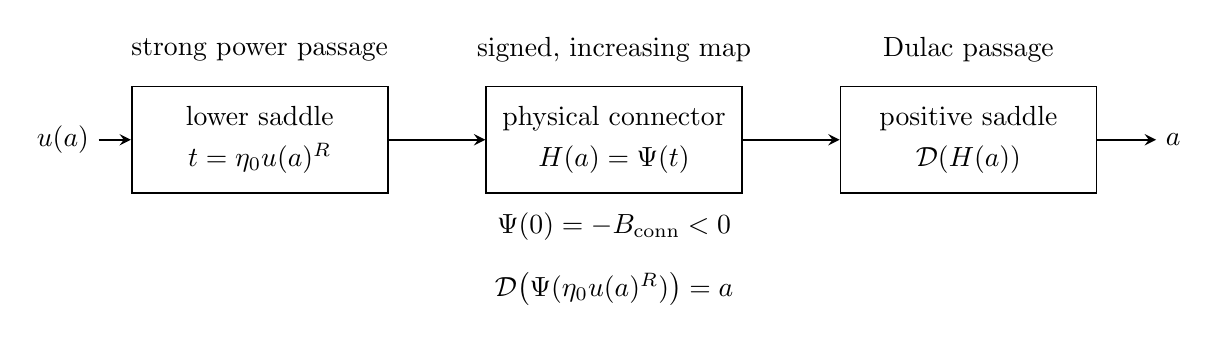
\begin{tikzpicture}[x=10mm,y=10mm,>=stealth,
  every node/.style={font=\fontsize{10}{12}\selectfont},
  block/.style={draw,line width=.6pt,minimum width=3.25cm,
    minimum height=1.35cm,align=center},
  map/.style={->,line width=.8pt}]
  \node (source) at (0,.2) {$u(a)$};
  \node[block] (lower) at (2.5,.2)
    {lower saddle\\[1mm]$t=\eta_0u(a)^R$};
  \node[block] (connector) at (7.0,.2)
    {physical connector\\[1mm]$H(a)=\Psi(t)$};
  \node[block] (positive) at (11.5,.2)
    {positive saddle\\[1mm]$\mathcal D(H(a))$};
  \node (target) at (14.1,.2) {$a$};
  \draw[map] (source)--(lower);
  \draw[map] (lower)--(connector);
  \draw[map] (connector)--(positive);
  \draw[map] (positive)--(target);
  \node at (2.5,1.35) {strong power passage};
  \node at (7.0,1.35) {signed, increasing map};
  \node at (11.5,1.35) {Dulac passage};
  \node at (7.0,-.9) {$\Psi(0)=-B_{\rm conn}<0$};
  \node at (7,-1.7)
    {$\mathcal D\!\left(\Psi(\eta_0u(a)^R)\right)=a$};
\end{tikzpicture}
\caption{Schematic composition of the complete negative-forcing two-endpoint return.
The arrows show the order of scalar maps, not phase-plane trajectories.
The full signed connector $\Psi$, with $\Psi(0)=-B_{\rm conn}<0$, is retained
in $H(a)=\Psi(\eta_0u(a)^R)$. The positive-saddle Dulac map is used on the
returning domain $H(a)>0$.}
\label{fig:two-saddle-connector}
\end{figure}


\subsection{Nonnegative forcing}

We prove attraction by estimating the complete-period multiplier.
The annulus count then gives the bound two.

Let $\mathfrak m$ be the characteristic multiplier of a positive cycle.
Since $z=(\log y)^{\boldsymbol\cdot}-\delta/y$, integration of the
divergence over a complete period gives the exact identity
\begin{equation}\label{eq:lower-multiplier}
 \log\mathfrak m
 =\oint\left[by-\varepsilon^2A
                  -(1+2\varepsilon^2C)\frac{\delta}{y}\right]dt.
\end{equation}
For $\delta\ge0$ the integrand is at most $by-\varepsilon^2A$.
The time spent near the left zero will dominate all positive contributions.
We estimate this time along the orbit, allowing reversals in $z$.

Choose fixed small $q,z_c,h_c>0$ such that the contact rectangle
$[-q,z_c]\times(0,h_c)$ satisfies
\begin{equation}\label{eq:lower-contact-box}
 1+bz-y\ge\tfrac12,\qquad F_y>0,\qquad P(-q)>p_q>0,
 \qquad |P(z)|\le A/(8b_+),
\end{equation}
where $b_+$ is an upper bound for $b$. The last two inequalities hold
after shrinking the coefficient neighborhood. The regular fast arc and
the descending passage to $y=K\varepsilon^3$ have uniformly bounded
positive contribution to \eqref{eq:lower-multiplier}. Indeed, on a fixed
negative interval, $G\le-c_0y$ for $y\ge K\varepsilon^3$, so a descent
from a fixed height $y_h$ contributes at most
$(b_+/c_0)\int_{K\varepsilon^3}^{y_h}dy$. The moving-entry estimate \eqref{eq:relaxation-map} gives
$\Lambda=\ell_b+O(\varepsilon^2(1+|\log\varepsilon|))$,
where $\ell_b$ is the regular fast-foot map.

Choose $H\ge K$ with $qH>\sup D$. Until the first subsequent hit of
$z=-q$, the boundary $y=H\varepsilon^3$ points downward. Thus the
positive cycle has $y\le H\varepsilon^3$ on this entire part of its
orbit, and the integrand in \eqref{eq:lower-multiplier} is at most
$-A_0\varepsilon^2/2$. This hit exists, since the same periodic orbit
must return to its upper fast section.

Put $f_*=f_{b_*}$ and fix $a>0$ with $f_*+a<-q$. For any sufficiently
small fixed $\tau>0$, shrink the coefficients and the fast source interval
so that $|\Lambda-f_*|\le\tau$ and
\[
 |P(z)|\le M(z-f_*+\tau)
       \quad(f_*+2\tau\le z\le f_*+a).
\]
Here $M$ can be chosen before $\tau$, since $P_*(f_*)=0$ and the
polynomial derivatives are bounded. Along the low orbit,
$|F|\le M\varepsilon^2(z-f_*+\tau+\varepsilon)$ on this strip.
To bound the crossing time even when $z$ reverses, use the function which equals
\[
 \log\frac{z-f_*+\tau+\varepsilon}{3\tau+\varepsilon}
\]
on the strip and is constant on each complementary half-line. Its
absolute time derivative is at most $M\varepsilon^2$. Its net change
between the descending entry and the first $-q$ hit is
$\log[(a+\tau+\varepsilon)/(3\tau+\varepsilon)]$. Consequently the
contribution of this whole low part is at most
\begin{equation}\label{eq:lower-log-time}
 -\frac{A_0}{2M}\log\frac{a}{4\tau},\qquad
 \varepsilon\le\tau.
\end{equation}
Leftward excursions do not affect this estimate: the function is constant
outside the strip, and its time derivative was estimated in absolute value.

At the first $-q$ hit the orbit enters the contact rectangle with
$F>0$. Its boundary clearances, positivity and $F_y>0$ give the
prescribed right exit with $F>0$ throughout, by the invariant-quadrant
argument in the proof of Lemma~\ref{lem:sections}.

Below $y_{\rm th}=\varepsilon^2A/(2b_+)$ the integrand of
\eqref{eq:lower-multiplier} is nonpositive. Above this height,
\eqref{eq:lower-contact-box} gives $F\ge y/4$. Its positive contact
contribution is therefore at most $4b_+(q+z_c)$. Fix all these positive
costs first, and then choose $\tau$ so that
\eqref{eq:lower-log-time} is smaller than their negative sum minus one.
Only afterward shrink the coefficients, source interval and
$\varepsilon_0\le\tau$. We obtain $\log\mathfrak m<-1$ for every
counted cycle, uniformly in all ratios of $c,D,\varepsilon$.
Choose $\mathcal A_-\Subset\mathcal A_+$ as in
Section~\ref{sec:graphic-anchored-annulus}, putting the larger annulus
inside the multiplier and section clearances and the counted cycles
and their intervening annuli in the smaller one. The estimate holds
throughout the ambient coefficient window for $D\ge0$.
Section~\ref{sec:ambient-genericity-window} supplies nondegenerate
perturbations with $D>0$, also from $D=0$. Lemmas~\ref{lem:equilibria}
and~\ref{lem:generic-attracting-index} now give the bound two.

\subsection{The lower passage for negative forcing}

The lower weak separatrix lies below $y=0$ for negative forcing.
We construct the transition from this negative baseline across the whole
power-output interval, with the first and second source derivatives
needed for the return comparison.

Assume henceforth that $\delta=-\nu<0$. At $y=0$ we have $G=-\nu$;
a trajectory which leaves $y>0$ cannot reenter it. This elementary sign
will also determine the displacement in the connection between the two
saddles.

Write $\mu:=\varepsilon^2$ for the slow scale and $\nu:=|\delta|$ for the
forcing magnitude. Below, $q$ is the physical ordinate on the outgoing
section, $u$ is the regular source coordinate, and $v$ is the normal
amplitude after the lower saddle passage.

\begin{lemma}\label{lem:lower-saddle-transition}
Let $q$ denote the physical ordinate on the outgoing section $z=z_c$;
we work on a fixed compact source interval in $q$, with the field
parameters $p$ held fixed.
Fix a small negative section $z=-q_0$ to the right of the lower polynomial
root. There are a regular source coordinate $u=u(q,p)$ and fixed
constants $\eta_0>0$, $0<\theta<1$, such
that every counted cycle has $0<u<\theta$ and reaches $-q_0$ with
ordinate
\begin{equation}\label{eq:lower-exact-transition}
 Y(q)=\Psi_-(\eta_0u(q)^R),\qquad
 R\asymp\varepsilon^{-2}.
\end{equation}
Here $p$ denotes the frozen field parameters,
\begin{gather}
 0<c_u\le u_q\le C_u,\qquad |u_{qq}|\le C_u,
 \label{eq:lower-regular-source}\\
 \Psi_-(v)=\beta_-+\kappa_-v[1+E(v/\varepsilon^2,p)],
 \qquad -M\nu\le\beta_-\le-m\nu<0,
 \label{eq:lower-signed-map}\\
 e^{-M/\varepsilon^2}\le\kappa_-\le e^{-m/\varepsilon^2},
 \qquad E(0,p)=0,\qquad \|E\|_{C^1}\le M .
 \label{eq:lower-signed-jets}
\end{gather}
The last norm is in the displayed amplitude variable, on a fixed small
interval; no parameter derivative is asserted. The signed map is $C^2$
on the whole interval $0\le v\le\eta_0\theta^R$. Its positive
part is one source interval, possibly empty. On this interval, after
shrinking $\varepsilon_0$,
\begin{equation}\label{eq:lower-flat-output}
 0<Y,Y_q\le M\varepsilon^{-2}e^{-m/\varepsilon^2},
 \qquad Y_{qq}\ge0,\qquad
 \nu\le M e^{-m/\varepsilon^2}\theta^R .
\end{equation}
\end{lemma}

\begin{proof}
Let $\beta<0$ be the lower root, so that $P'(\beta)>p_0>0$.
Set $\mu=\varepsilon^2$, fix the required final order $j\ge8$, and
first construct the invariant graph with additional phase derivatives.
For $\nu>0$, the substitution $y=\nu\zeta$ gives
\[
 \dot z=\nu\zeta(1+bz-\nu\zeta)+\mu P(z),\qquad
 \dot\zeta=z\zeta-1.
\]
These polynomial equations extend regularly to $\nu=0$.
The physical graph is recovered by $h=\nu\zeta$, which degenerates at
that parameter value.
At $\mu=\nu=0$, the graph $\zeta=1/z$ on the fixed negative
interval is normally attracting with a fixed spectral gap. Embed this
interval in a fixed compact boundaryless base and extend the graph and
field there, using a cut-off independent of the frozen field parameters.
Writing $w=\zeta-1/z$, the extended critical field has
$\dot z=0$ and $\dot w=a_0(z)w$ on $w=0$, with
$a_0\le-\sigma<0$. For a fixed order $r\ge 2j+12$, on a common tube
and uniformly in the frozen parameters,
$\|\dot z\|_{C^r}+\|\dot w-a_0(z)w\|_{C^r}\le C(\mu+\nu)$.
The compact boundaryless graph therefore has zero tangential rate and a
uniform normal gap. After one common shrinking of the parameter box,
Fenichel's compact normally-hyperbolic persistence theorem,
\cite[Theorem~3, p.~215]{Fenichel1971}, gives a persistent invariant
$C^r$ graph $\zeta=k(z;\mu,\nu,p)$ in a common tube.
The differentiated-maximum argument in the proof of
Lemma~\ref{lem:pc-selected-graph} applies with transport size
$\mu+\nu$ and normal coefficient $a_0\le-\sigma<0$; reversing its
sign does not change the absolute-value estimate. With
$r\ge2j+12$ it yields
$\|k-z^{-1}\|_{C^{2j+11}}\le C_j(\mu+\nu)$ on the extended circle.
Restrict the graph to
the nested working interval, where the extension agrees with the original
field. At $\nu=0$ its physical reconstruction is $h=\nu k\equiv0$.
The invariance equation gives the quantitative estimate:
\[
 zk-1=k_z\{\nu k(1+bz-\nu k)+\mu P(z)\}.
\]
Thus $k-z^{-1}=O_{C^{2j+10}}(\mu+\nu)$ and $h=\nu k$ satisfies
\begin{equation}\label{eq:lower-slow-graph}
 h(z)=\nu\{z^{-1}+O_{C^{2j+10}}(\mu+\nu)\},
 \qquad h<0\ \text{for }\nu>0,
\end{equation}
with the regular limiting choice $h\equiv0$ at $\nu=0$. Only phase derivatives, with the field fixed,
are used below. Notice also that $\nu/\mu=\varepsilon|D|\to0$
already follows from the normalization; it does not require the later
exponentially small survival estimate.

Translate the chosen graph by $w=y-h(z)$ and put
$q_n(z,w)=1+bz-2h(z)-w$. The exact equations are
\[
 \dot z=\mu\mathcal V(z)+q_n(z,w)w,\qquad
 \dot w=(z-h_zq_n(z,w))w,\qquad
 \mathcal V=P+\frac{h(1+bz-h)}\mu.
\]
The coefficients have common $C^{2j+8}$ bounds,
$\mathcal V=P+O_{C^{2j+8}}(\nu/\mu)$,
and the normal coefficient is bounded above by a negative constant.
Lemma~\ref{lem:uniform-normal-product} applies with $\tau=\mu$ and
$\rho=1$, at order $j+1$. It gives an exact product, preserving this particular graph,
with uniformly transverse normal coordinate.

The equilibrium on this graph lies at $z=\beta+O(\nu/\mu)$ and
has a negative eigenvalue bounded away from zero and a positive eigenvalue
comparable with $\mu$. The graph through it agrees to its right with
its weak unstable separatrix. Since $\mathcal V'$ is a positive unit at its
simple zero, the scalar change following
Lemma~\ref{lem:uniform-normal-product}, after division by the absolute
normal rate, gives
\begin{equation}\label{eq:lower-product}
 \dot\xi=\mu b_w\xi,\qquad\dot\eta=-\eta,\qquad 0<m_w<b_w<M_w .
\end{equation}
The coordinate $\xi$ increases to the right of the equilibrium.
This is an exact finite-order orbital normal form; its construction
does not divide by the small eigenvalue.

Choose the incoming cut $\eta=\eta_0>0$ and an outgoing weak cut
$\xi=\xi_{\rm out}>0$. The regular fast orbit reaches the incoming
cut in bounded time. Its weak coordinate, divided by $\xi_{\rm out}$,
is $u(q)$. The Poincar\'e determinant formula gives
\eqref{eq:lower-regular-source}, with positive orientation in physical
ordinate $q$: both transverse determinants are positive. After fixing
both weak exits, shrink the source so that their normalized absolute
incoming coordinate is less than $\theta<1$. The right local output is
exactly $v=\eta_0u^R$, with $R=(\mu b_w)^{-1}$.
For $u=0$ the orbit approaches the saddle below $y=0$. For $u<0$ its
left output is at most $\eta_0\theta^R$. Choose a fixed physical line
$z=z_{\rm left}$ left of all lower roots, with
$P(z_{\rm left})<-p_{\rm left}<0$. The still-positive left output has
height $o(\mu)$ there. For a small fixed $h_{\rm left}>0$, the half-strip
$z\le z_{\rm left}$, $0<y\le h_{\rm left}\mu$ has inward flow on its
right and upper sides. It cannot return to the positive outgoing section.

We next transfer the weak outgoing cut to a fixed physical vertical
section $z=z_l$, retaining the derivative loss caused by the slow speed.
Write the inverse coordinates as
$(z,y)=(X(\xi,\eta),H(\xi,\eta))$ and choose
$X(\xi_{\rm out},0)=z_l$. The nearby occurrence on that physical line
is determined by
\[
 X(\xi_{\rm out}e^{\mu b_wt},ve^{-t})=z_l.
\]
For $0\le v\le c_0\mu$, with $c_0>0$ fixed and small, its time derivative
is comparable with $\mu$. The normal direction is uniformly transverse,
and the weak exit stays a fixed distance from the base root. The
$\rho=1$ section change \eqref{eq:uniform-physical-section}, with
$v=\mu V$, therefore gives
\begin{equation}\label{eq:lower-cut-change}
 \Phi(v)=h(z_l)+a_lv+(v^2/\mu)E_l(v/\mu),\qquad
 a_l=H_\eta-h_zX_\eta>0,\qquad \|E_l\|_{C^{j-3}}\le M.
\end{equation}
In particular $\Phi'$ is bounded above and below by positive constants,
and $\Phi''/\Phi'=O(\mu^{-1})$. The actual argument range
$v\le\eta_0\theta^R$ is exponentially smaller than $\mu$.

On $[z_l,-q_0]$ the polynomial is uniformly positive. The signed tube
about $h$ has $F\asymp\mu$. For the scalar equation
$y_z=\mathcal R(z,y)=(zy-\nu)/F$,
\begin{equation}\label{eq:lower-scalar-derivative}
 \mathcal R_y=
 \frac{z(y^2+\mu P)+\nu(1+bz-2y)}{F^2},\qquad
 -M/\mu\le\mathcal R_y\le-m/\mu,
\end{equation}
and $|\partial_y^j\mathcal R|\le M_j\mu^{-j}$ for $j\ge2$.
Positivity at the lower right cut requires $\nu\le M\theta^R$, in
addition to $\nu/\mu\to0$. To define the transition also for signed
inputs, use the estimate on $\mathcal R_y$: it makes the tube
$|y-h(z)|\le c_1\mu$ forward invariant, for fixed small $c_1>0$.
After decreasing $c_0$, it contains the image of $\Phi$ on
$0\le v\le c_0\mu$. Thus the signed transition is defined on this whole
interval, not only on the exponentially short range of counted orbits.
Write its scalar part as $y(z,w)$ with $y(z_l,w)=w$, and put
$J=y_w$ and $L=(\log J)_w$. Their variational equations are
\begin{equation}\label{eq:lower-relative-variations}
 (\log J)_z=\mathcal R_y,\qquad L_z=\mathcal R_{yy}J,
 \qquad J(z_l)=1,\quad L(z_l)=0.
\end{equation}
Since $0<J\le e^{-m(z-z_l)/\mu}$, integration gives
$|y_{ww}/y_w|=|L|\le M\mu^{-1}$.
Composition with \eqref{eq:lower-cut-change} yields
$|\Psi_-''/\Psi_-'|\le M\mu^{-1}$.
Its baseline is $\beta_-=h(-q_0)$, between two fixed negative multiples
of $\nu$, and \eqref{eq:lower-scalar-derivative} gives the stated
exponential bounds for $\kappa_-=\Psi_-'(0)$. Moreover
$\Psi_-'(v)/\kappa_-$ is bounded above and below on $0\le v\le c_0\mu$.
For $V=v/\mu$, the exact formula
\[
 E(V,p)=\int_0^1
       \left\{\frac{\Psi_-'(t\mu V)}{\kappa_-}-1\right\}dt
\]
therefore gives $E(0,p)=0$ and a uniform $C^1$ bound on $0\le V\le c_0$.
This proves
\eqref{eq:lower-signed-map}--\eqref{eq:lower-signed-jets}.

The map $\Psi_-$ is increasing. Positivity at its target is equivalent
to positivity throughout the preceding orbit, because $G(z,0)<0$.
Hence $Y>0$ selects one upper interval and implies the last inequality
of \eqref{eq:lower-flat-output}. Finally, with $v=\eta_0u^R$,
\[
 \frac{Y_{qq}}{Y_q}
  =(R-1)\frac{u_q}{u}+\frac{u_{qq}}{u_q}
           +\frac{\Psi_-''}{\Psi_-'}R v\frac{u_q}{u}.
\]
The last term is bounded by $M R(v/\mu)u_q/u$ and is absorbed by the
first term on the whole interval. This proves convexity and the remaining
bounds in \eqref{eq:lower-flat-output}.
\end{proof}

\subsection{Positive outlets and local passages}

We first exclude contact constants bounded away from zero on the
negative scaled side, then treat the saddle-node range. For the remaining
positive outlets we construct reference orbits of the same field.
Their continuation to the physical section supplies the source derivative
bounds used in both the saddle-node and two-saddle returns.

Set
\begin{equation}\label{eq:lower-contact-parameters}
 k=\frac{c}{\varepsilon^2},\qquad
 \ell=-\frac{\nu}{A^3\varepsilon^6}.
\end{equation}
The survival inequality in \eqref{eq:lower-flat-output} implies
$\ell\to0$ uniformly whenever a counted cycle exists. For any fixed
$k_0>0$, the fields with $k\le-k_0$ have no such cycle. Indeed, on
the line $z_g=Ac/2<0$,
\[
 P(z_g)=A^2(c/2+Cc^2/4)\le-A^2|c|/4.
\]
At heights $0\le y\le h_g=A^2\varepsilon^2|c|/16$ the field points
left. Since $h_g\ge A_0^2k_0\varepsilon^4/16$, the output of
Lemma~\ref{lem:lower-saddle-transition} lies below this height for small
$\varepsilon$. The strip $z\le z_g$, $0<y\le h_g$ also points
inward on its upper side, and a downward exit cannot be reversed. This
argument includes $k\to-\infty$.

For $|k|$ small put $n=A\varepsilon^2$, $z=nU$, $y=n^2V$.
The exact equations are
\begin{equation}\label{eq:lower-epsilon-equations}
 U'=V(1+bnU-n^2V)+k-U+C\varepsilon^2U^2,\qquad V'=UV+\ell .
\end{equation}
Fix a small $d_0>0$, and choose $|k|\le k_c<d_0/8$ and
$|C|q_0\le A_0/8$. Then
\[
 P(-x)\ge\tfrac34 Ax,\qquad d_0A\varepsilon^2\le x\le q_0.
\]
Every still-positive lower output decreases in height while $z<0$.
It is exponentially smaller than $\varepsilon^2P$ down to $U=-d_0$,
so $F\ge\varepsilon^2P/2>0$ there. It either reaches this section
in finite time or first hits $y=0$. In the former case its ordinate and
first derivative in the scaled coordinate satisfy
\begin{equation}\label{eq:lower-central-small-entry}
 V=o(1),\qquad
 0<V_q\le M\varepsilon^{-6}e^{-m/\varepsilon^2}
       =:\zeta_\varepsilon\longrightarrow0,\qquad V_{qq}\ge0.
\end{equation}
Here convexity is preserved on the small negative tail. Indeed, direct
differentiation gives, with $Q=1+bz$,
\[
 \mathcal R_{yy}
 =\frac{2\{z[y^3+(3y-Q)\varepsilon^2P]
       -\nu[\varepsilon^2P+Q^2-3Qy+3y^2]\}}{F^3}>0,
\]
whereas $\mathcal R_y<0$ by \eqref{eq:lower-scalar-derivative}.
The forcing term is absorbed because
$\nu/(|z|\varepsilon^2P)\le M\nu\varepsilon^{-6}\to0$.
Only this small contact interval, where $Q>0$, is assigned a convexity
sign; the remote negative interval was included in $\Psi_-$.

Apply the finitely differentiable product coordinates of
Lemma~\ref{lem:saddle-node-passage} to \eqref{eq:lower-epsilon-equations}.
Write them as $\dot s=W(s,p)$, $\dot w=-w$, with center value
$\sigma(p)$. At $k=\ell=0$ the strong line is $V=0$, and
$s=V\chi(U,V)$ with $\chi>0$. Consequently the entries in
\eqref{eq:lower-central-small-entry} have
\[
 3d_0/4<w<5d_0/4,\qquad |s-\sigma|\le M(V+|k|+|\ell|).
\]
The fixed strong cut $w=w_0=d_0/2$ is reached in time
$\log(w/w_0)$, bounded above and below by positive constants. Its
coordinate is an increasing $C^3$ function of $V$, with bounded
logarithmic curvature. Thus the complete map $N(q)$ from the original
physical section to this cut satisfies
\begin{equation}\label{eq:lower-central-complement}
 N_q>0,\qquad \sup N_q\le M\zeta_\varepsilon,\qquad
 N_{qq}/N_q\ge-M\zeta_\varepsilon .
\end{equation}

The next lemma supplies the reference graphs and transverse incidence
required by Lemma~\ref{lem:positive-transition}. Applying that transition
lemma then gives the outgoing estimates on a fixed relative neighborhood
of each reference.

\begin{lemma}\label{lem:lower-positive-references}
Choose the fixed physical section $z=z_c>0$ before the final parameter
shrinking.  For every field admitting a counted lower passage, the
following three outgoing orbits continue to $z=z_c$:
\begin{enumerate}
 \item the zero-stable-amplitude orbit from the right exit of the
       saddle-node product box, for $|k|\le k_c$;
 \item the outgoing unstable separatrix of the positive saddle, for
       $k\in[k_c,K_1]$;
 \item the outgoing unstable separatrix of the small-ratio saddle, for
       $e=\varepsilon/\sqrt c\le e_0$.
\end{enumerate}
After the corresponding compact local outlet change, put
$z=nU$, $y=n^2V$, with $n=A\varepsilon^2$ in the first two cases and
$n=Ac$ in the third.  Each reference is a graph $V=h(U)$ on a fixed
positive scaled section and satisfies, up to $z=z_c$,
\begin{equation}\label{eq:lower-positive-reference-bounds}
 c_h(1+U^2)\le h(U)\le C_h(1+U^2),\qquad
 \mathcal F(U,h)\ge c_Fh,
\end{equation}
where $\mathcal F$ is the horizontal component of the scaled field.
The local outgoing amplitude $a$ can be oriented so that on the initial
reference section
\begin{equation}\label{eq:lower-positive-reference-incidence}
 g(a):=\frac{V(a)}{h}-1,\qquad g(0)=0,\qquad
 0<c_g\le g'\le C_g,\qquad |g''|+|g'''|\le C_g.
\end{equation}
All constants are uniform on the stated ranges.  Thus the reference and
initial-incidence hypotheses of Lemma~\ref{lem:positive-transition}
hold in its applications below.
\end{lemma}

\begin{proof}
All three cases reduce, after the local outlet change, to
\begin{equation}\label{eq:lower-positive-reference-system}
 \dot U=\mathcal F(U,V)=VQ(U,V)+p(U),\qquad
 \dot V=UV+\ell_*,\qquad Q=1+bnU-n^2V.
\end{equation}
For the first two cases
\[
 p(U)=k-U+C\varepsilon^2U^2,\qquad
 n=A\varepsilon^2,\qquad \ell_*=-\nu/n^3,
\]
whereas in the small-ratio case
\[
 p(U)=e^2(1-U)+C\varepsilon^2U^2,\qquad
 n=Ac,\qquad \ell_*=e^3\eta=-\nu/n^3.
\]
The survival estimate \eqref{eq:lower-flat-output} implies
$\ell_*\to0$ in all three cases and $\eta\to0$ in the last, since the
denominators lose at most a fixed power of $\varepsilon$.  Fix a small
$\varrho>0$.  After choosing $z_c$ and then shrinking the parameters,
\begin{equation}\label{eq:lower-positive-reference-Q}
 1-\varrho\le Q\le1+\varrho
\end{equation}
whenever $0\le z\le z_c$ and $y\le C(n^2+z^2)$.
The upper barriers below give this height bound and close the first-exit
argument on the chosen physical rectangle.

At the saddle-node organizer $k=\ell_*=\varepsilon=0$, the outgoing
center graph satisfies
\[
 h_0(U)=U+U^2+O(U^3),\qquad
 \mathcal F(U,h_0)=U^2+O(U^3).
\]
Fix a small $\delta>0$ and choose the right product exit so that its
zero-stable-amplitude orbit reaches $U=\delta$.  Finite smooth dependence
of the product and section coordinates gives
\begin{equation}\label{eq:lower-central-reference-entry}
 \begin{aligned}
 h(\delta)&=\delta+\delta^2
       +O(\delta^3+|k|+|\ell_*|+\varepsilon^2),\\
 \mathcal F(\delta,h(\delta))&=\delta^2
       +O(\delta^3+|k|+|\ell_*|+\varepsilon^2).
 \end{aligned}
\end{equation}
Decrease the previously chosen $k_c$, if necessary, so that
$k_c\le\kappa_0\delta^2$, and then shrink $\varepsilon$ and the forcing.
For $m_0=1+\delta/4$, the line $L_1=m_0U$ starts below the reference.
Its exact inward-crossing expression is
\begin{equation}\label{eq:lower-central-reference-linear}
 \begin{split}
 (UL_1+\ell_*)-L_1'\mathcal F(U,L_1)
 =m_0\{&(1-C\varepsilon^2-m_0bn+m_0^2n^2)U^2\\
       &-(m_0-1)U-k\}+\ell_*>0,
 \end{split}
\end{equation}
for $U\ge\delta$.  A fixed sufficiently small
$L_2=\gamma(1+U^2)$ is also a lower barrier: at a first meeting,
\[
 (UL_2+\ell_*)-L_2'\mathcal F(U,L_2)
 \ge UL_2\{1-2\gamma(1+\varrho+|C|\varepsilon^2/\gamma)\}
       -|\ell_*|-2\gamma U|k|>0.
\]
A fixed sufficiently large $H_2=M(1+U^2)$ is an upper barrier, since
$\mathcal F(U,H_2)\ge H_2/2$ and, at a first upward meeting,
\[
 \frac{UH_2+\ell_*}{\mathcal F(U,H_2)}<H_2'.
\]
The two lower barriers give
\begin{equation}\label{eq:lower-central-reference-speed}
 \frac{\mathcal F(U,h)}h
 \ge1-\varrho-\frac1{m_0}
       -\frac{|k|}{m_0\delta}-\frac{|C|\varepsilon^2}{\gamma}
 \ge c_F>0.
\end{equation}
The barriers and positive speed prove
\eqref{eq:lower-positive-reference-bounds} in the saddle-node range and
continue the reference to $z=z_c$.
The product coordinates may be oriented at the organizer by
$s=V+O(2)$ and $w=V-U+O(2)$.  Increasing the outgoing amplitude is then
positively transverse to the flow; the Poincar\'e determinant formula
and the compact transition to $U=\delta$ give
\eqref{eq:lower-positive-reference-incidence}.

For $k\in[k_c,K_1]$, let $(U_s,V_s)$ be the positive saddle and let $h$
be its actual outgoing unstable separatrix.  Choose a new fixed
$\delta_b\ll k_c$.  Uniform hyperbolicity gives on $U=U_s+\delta_b$
\begin{equation}\label{eq:lower-bounded-reference-entry}
 h=(1+k)\delta_b+O(\delta_b^2+\varepsilon^2+|\ell_*|),\qquad
 \mathcal F=k\delta_b+O(\delta_b^2+\varepsilon^2+|\ell_*|).
\end{equation}
Put $m_1=1+k_c/2$ and $t=U-U_s$.  The line
$L_1=m_1t$ begins below $h$, and its exact crossing expression is
\begin{equation}\label{eq:lower-bounded-reference-linear}
 (UL_1+\ell_*)-L_1'\mathcal F(U,L_1)
 =m_1t[U+1-m_1Q]-m_1(k-U_s)
      -m_1C\varepsilon^2U^2+\ell_*.
\end{equation}
On the compact $k$-interval the first term has a fixed positive lower
bound proportional to $t(1+U)$; it absorbs all remaining terms after
the parameter shrinking.  The same parabolic lower and upper barriers
as above give
\[
 \gamma(1+U^2)\le h(U)\le M(1+U^2),\qquad
 \frac{\mathcal F(U,h)}h
 \ge1-\varrho-\frac1{m_1}
      -\frac{|k-U_s|}{m_1\delta_b}-\frac{|C|\varepsilon^2}{\gamma}
 \ge c_F.
\]
Continue first from the parameter-dependent line $U=U_s+\delta_b$ to a
fixed $U_0>K_1+2\delta_b$.  This is a uniformly transverse compact
transition, after which the barriers continue to $z=z_c$.
The saddle separatrices and these fixed section maps have common finite
derivatives; orienting the outgoing amplitude by the positive transverse
determinant proves \eqref{eq:lower-positive-reference-incidence}.

It remains to construct the small-ratio reference.  In the variables of
\eqref{eq:lower-small-ratio}, its selected local outlet is the actual
outgoing unstable separatrix.  Continue it by a bounded local map to the
fixed horizontal level $Y=d_1>0$, where $X$ lies in a fixed positive
compact interval and $e|\eta|\ll d_1$.  Using $Y$ as phase until
$Y=e^{-2}$, one has
\[
 \frac{dX}{dY}=\frac{e^2\mathcal F_s}{XY+e\eta},\qquad
 \mathcal F_s=Y(1+bnX-n^2e^2Y)+1-X+CcX^2.
\]
The initially positive $\mathcal F_s$ cannot first vanish: at such a
point the term containing $X_Y$ vanishes and
\[
 \frac{d\mathcal F_s}{dY}=1+bnX-2n^2e^2Y>\tfrac12.
\]
Moreover $XY+e\eta\ge cXY$ and
\[
 \frac{d(X^2)}{dY}
 \le Ce^2(1+Y^{-1})+Cce^2X^2/Y.
\]
Gronwall's inequality gives positive uniform upper and lower bounds for
$X$ at $Y=e^{-2}$.  In the common variables this is the fixed horizontal
level $V=e^2Y=1$.  Continue to a fixed $U_0$ to its right; on that compact
piece $\mathcal F$ and $UV+\ell_*$ are positive units.  For $U\ge U_0$,
the barriers $\gamma(1+U^2)$ and $M(1+U^2)$ give
\[
 \gamma(1+U^2)\le h(U)\le M(1+U^2),\qquad
 \frac{\mathcal F(U,h)}h
 \ge1-\varrho-\frac{e^2U}{\gamma(1+U^2)}
             -\frac{|C|\varepsilon^2}{\gamma}\ge c_F.
\]
This proves \eqref{eq:lower-positive-reference-bounds} in the third case.

Finally orient its local amplitude so that increasing $a$ decreases the
outlet $X$ by a positive unit.  The $Y$-phase map has positive-unit first
variation and bounded derivatives through order three, since the relevant
coefficients have the integrable majorant $Ce^2(1+Y^{-1})$.  If $x(a)$
is the abscissa at $V=1$, then $x'(a)<-c<0$.  Differentiating the scalar
flow from this moving initial point to fixed $U_0$ gives
\[
 \partial_xV(U_0;x)
 =-\frac{x+\ell_*}{\mathcal F(x,1)}
   \exp\left(\int_x^{U_0}\partial_V
       \frac{UV+\ell_*}{\mathcal F(U,V)}\,dU\right)<0.
\]
All factors are positive units; hence $V_a(U_0)>0$ is a unit, and the
first three differentiated equations give
\eqref{eq:lower-positive-reference-incidence}.
As the scale and coefficient parameters approach the organizer, the
three references and their fixed relative collars converge on compact
subsets of $0<z\le z_c$ to its outgoing fast orbit. The small-ratio limit
here includes $c\to0$; for fixed nonzero small $c$, the fast limit may
start at the displaced positive root. In the joint limit the parabolic
bounds give zero height at $z=0$, and uniqueness for the regular fast
scalar equation identifies the limit. Thus, after first making the
coefficient neighborhood small enough, all references and collars reach
the same fixed transverse target inside its regular physical flow box.
This supplies the common target and its positive clearance for the return
construction.
\end{proof}

\paragraph{The saddle-node return.}
Return to the saddle-node passage and choose the right product exit
$s=s_+$ with $W(s_+)>0$.
The only entries which reach it have $[s,s_+]\subset\{W>0\}$;
they form one interval, to the right of the last root if roots are present.
The local map and its exact differential identity are
\begin{equation}\label{eq:lower-node-map}
 \mathcal D(s)=w_0\exp\left[-\int_s^{s_+}\frac{d\tau}{W(\tau)}\right],
 \qquad W\mathcal D'=\mathcal D .
\end{equation}
Let $C_+(a)$ be the continuation from this exit to the physical section.
Part~(1) of Lemma~\ref{lem:lower-positive-references} verifies the actual
reference and its positive-unit incidence.  Lemma~\ref{lem:positive-transition}
therefore gives $C_+'>0$ and bounded
$C_+''/C_+'$ and $C_+'$. For $H=N\circ C_+$,
\[
 aH''/H'\ge-Ma-Ma\zeta_\varepsilon\ge-M_1a.
\]
Fix the product box with $W_s\le1/4$, then $a_0$ with
$M_1a_0\le1/4$. The passage estimate in
Lemma~\ref{lem:saddle-node-passage} places every local output below
$a_0$ once its entry is sufficiently close to $\sigma$; choose $k_c$
and then $\varepsilon_0$ accordingly. Thus \eqref{eq:simple-pfaff-hypothesis} holds with margin $1/2$.
Lemma~\ref{lem:saddle-node-passage} gives total isolated return-zero
multiplicity at most two, including an exactly quadratic stationary zero.
The finite-passage domain is one interval, obtained from increasing maps:
positive lower output, positive entry at the strong cut, the unique
component of $W>0$ reaching $s_+$, and the original physical section
interval. The comparison therefore applies throughout this actual domain.

\paragraph{The positive Dulac map.}
We now prepare the positive-saddle passage for
Lemma~\ref{lem:flat-two-saddle-comparison}.
It suffices to consider fields admitting a counted cycle, so that the
survival bound in \eqref{eq:lower-flat-output} holds.
In the range $k\in[k_c,K_1]$, equation~\eqref{eq:lower-epsilon-equations}
gives a positive saddle with eigenvalues near $-1$ and $k$, and ordinate
$-\ell/U_s>0$. For large $k$, put
\begin{equation}\label{eq:lower-small-ratio}
 e=\varepsilon/\sqrt c,\quad n=Ac,\quad
 z=nX,\quad y=n^2e^2Y,\quad \eta=-\nu/(n^3e^3).
\end{equation}
Here $c\ge K_1\varepsilon^2$ and $A\ge A_0$, so the survival bound
implies $|\eta|\le M\varepsilon^{-6}e^{-m/\varepsilon^2}\to0$.
The equations become
\[
 X'=e^2\mathcal F,\quad
 \mathcal F=Y(1+bnX-n^2e^2Y)+1-X+CcX^2,\qquad
 Y'=XY+e\eta.
\]
The saddle near $(1,0)$ has characteristic ratio $r=e^2\beta_s$,
where $\beta_s$ is bounded above and below by positive constants.
Lemma~\ref{lem:small-ratio-saddle} applies with the present bounded
negative $C$ and the chosen stable graph. Its use of
Lemma~\ref{lem:uniform-normal-product} has $\tau=\rho=e^2$ and a
fixed positive normal gap, or a negative gap in reversed time. It gives
the exact $C^j$ orbital normal form
\begin{equation}\label{eq:lower-positive-product}
 \dot\xi=-r\xi,\qquad\dot\omega=\omega,\qquad
 \mathcal D(s)=\xi_0(s/\omega_0)^r.
\end{equation}
The stable graph is $Y=-e\eta/X+O_{C^j}(e^3|\eta|)>0$ and the
strong-fiber slope in $X$ is $O_{C^{j-1}}(e^2)$.


\subsection{The signed connector and the two-saddle return}

For $k\ge k_c>0$, the connector must carry the lower power output to the
positive saddle. When its characteristic ratio is small, this passage
can amplify height and derivatives by an exponential factor. The lower
contraction must dominate that factor on the whole signed input interval.
The next proposition proves this domination, preserves the negative
baseline, and bounds the weighted logarithmic curvature needed by
Lemma~\ref{lem:flat-two-saddle-comparison}.

\begin{proposition}[The complete signed connector]
\label{prop:complete-signed-connector}
Fix the compact coefficient window in \eqref{eq:lower-family}, the finite
phase order, and the selected lower graph and positive-saddle coordinates
constructed above. The lower weak unstable branch is the zero source;
the incoming unstable coordinate increases with physical height from
the positive saddle's stable branch. Fix $k_c>0$, a small-ratio threshold
$e_0>0$, and $K_1\ge\max\{k_c,e_0^{-2}\}$.
For each final choice of the lower power-output cut and compatible
canonical incoming cuts within the fixed saddle cores, take
$\eta_0>0$, $0<\theta<1$, $R\asymp\varepsilon^{-2}$ and the survival
constants $C_s,m_s>0$ from Lemma~\ref{lem:lower-saddle-transition} and
\eqref{eq:lower-flat-output}. There are $\bar c,\varepsilon_0>0$ such
that every field in this window satisfying
\[
 \delta=-\nu<0,\qquad
 0<\varepsilon<\varepsilon_0,\quad 0<c<\bar c,\quad
 k=c/\varepsilon^2\ge k_c,\qquad
 0<\nu\le C_s\theta^R e^{-m_s/\varepsilon^2}
\]
has the following connector. Put $t_*=\eta_0\theta^R$.
The forward flow from the entire lower power-output interval
$0\le t\le t_*$ reaches the selected canonical incoming section of the
positive saddle in finite positive time. Its unstable coordinate defines
$\Psi\in C^2([0,t_*])$ with
$\Psi(0)=-B_{\rm conn}<0$ and $\Psi'>0$, and
\begin{equation}\label{eq:lower-connector-C2}
 \eta_0\sup_{[0,t_*]}\Psi'\le1,\qquad
 \left|t\frac{\Psi''(t)}{\Psi'(t)}\right|\le1
 \quad(0<t\le t_*).
\end{equation}
The estimates are uniform for these fields; all source derivatives are
taken with the vector field fixed.
\end{proposition}

\begin{proof}
Continue the whole signed interval $0\le v\le\eta_0\theta^R$
from Lemma~\ref{lem:lower-saddle-transition} to the canonical incoming
section of the positive saddle. Put $\mu=\varepsilon^2$.
The signed lower transition and the assumed survival bound give, with
$0<\theta<1$,
\begin{equation}\label{eq:lower-connector-input}
 |Y(-q_0)|\le M(\theta^R+\nu),\quad
 \nu\le M\theta^R e^{-m/\mu},\quad R\ge r_-/\mu,
\end{equation}
where $Y(-q_0)=\Psi_-(v)$. On this $v$-interval,
$0<\Psi_-'(v)\le M e^{-m/\mu}$, and
$|\Psi_-''(v)/\Psi_-'(v)|$ is bounded
by a fixed power of $\varepsilon^{-1}$. With the finite phase order,
$e_0$, $K_1$, the saddle cores and root gap fixed, choose the cuts and
tube widths before the upper bound $\bar c$ for $c$. The restrictions
\begin{equation}\label{eq:lower-connector-geometry}
 LA_1\bar c<q_0,\qquad LA_1\varepsilon_0^2<q_0
\end{equation}
are imposed before shrinking $\varepsilon_0$.

Choose $q_0$ smaller, if necessary, so that
\begin{equation}\label{eq:lower-connector-P}
 P(-x)\ge \frac78Ax+A^2c\qquad(0\le x\le q_0).
\end{equation}
In the bounded-ratio range set $n=A\varepsilon^2$ and in the small-ratio
range set $n=Ac$.  Thus $n\ge c_n\varepsilon^2$.  With
\[
 \omega_\varepsilon=K\{\theta^R+\nu/n\},
\]
choose $K$ larger than twice the constant in
\eqref{eq:lower-connector-input}, and then require $LK>2$, $n<1$, and
$\omega_\varepsilon<1/2$.  Let $B_1,C_Q$ bound respectively
$|1+bz-y|$ and $|1+bz-2y|$ on the contact box.  Since the right side of
\eqref{eq:lower-connector-P} is bounded below by a fixed multiple of
$n$, polynomial losses in $\varepsilon^{-1}$ are dominated by the
exponential factors in \eqref{eq:lower-connector-input}; hence we may impose
\begin{equation}\label{eq:lower-connector-smallness}
 B_1\omega_\varepsilon\le \frac{\varepsilon^2}{4}
       \min_{Ln\le x\le q_0}P(-x),\qquad
 C_Q\nu\le \frac{x\varepsilon^2P(-x)}{4}
       \quad(Ln\le x\le q_0).
\end{equation}
For $z=-x$ and $|y|\le\omega_\varepsilon$, (\ref{eq:lower-connector-smallness})
therefore gives
\begin{equation}\label{eq:lower-connector-F}
 \frac12\varepsilon^2P(z)\le F(z,y)
 \le \frac32\varepsilon^2P(z).
\end{equation}
The upper horizontal face has $G=-x\omega_\varepsilon-\nu<0$, while the
lower face satisfies
\[
 G=x\omega_\varepsilon-\nu\ge xK\theta^R+(LK-1)\nu>0.
\]
Thus the signed interval reaches $z=-Ln$ inside this strip.  For
$\mathcal R=G/F$ an exact differentiation gives
\begin{equation}\label{eq:lower-connector-Ry}
 \mathcal R_y=\frac{z(y^2+\varepsilon^2P)+\nu(1+bz-2y)}{F^2}<0.
\end{equation}
If $J=y_{y_0}$ and $L_2=y_{y_0y_0}/J$, then
\begin{equation}\label{eq:lower-connector-variations}
 J_z=\mathcal R_yJ,\qquad (L_2)_z=\mathcal R_{yy}J.
\end{equation}
Since $0<J\le1$ and the coefficients of $\mathcal R$ are bounded by fixed
powers of $\varepsilon^{-1}$, integration bounds $L_2$ by such a power.
For the terminal map $H(y_0)=y(-Ln;y_0)$ and $g=H\circ\Psi_-$,
\[
 \frac{H''}{H'}=L_2,\qquad
 \frac{g''}{g'}=(L_2\circ\Psi_-)\Psi_-'
                         +\frac{\Psi_-''}{\Psi_-'}.
\]
Thus passage to the inner scale preserves exponential contraction of
the first derivative and introduces only polynomial growth in the
relative second derivative.

For $k\in[k_c,K_1]$, use $n=A\varepsilon^2$, $z=nU$, $y=n^2V$ and
$\ell=-\nu/(A^3\varepsilon^6)$. Write
\[
 F_b(U,V)=V(1+bnU-n^2V)+k-U+C\varepsilon^2U^2
\]
for the horizontal component of \eqref{eq:lower-epsilon-equations}.
On $[-L,0]$ and $[0,U_s-\sigma]$, where $U_s$ is its positive
zero at $V=0$, one has $F_b(U,0)\ge c_*>0$ after shrinking
$\varepsilon$.
Writing $D_\varepsilon=|V(-L)|+|\ell|$, a first-exit tube
$|V|\le K_{\rm Gr}D_\varepsilon$ (with $K_{\rm Gr}$ larger than the fixed
Gronwall constant)
closes because the $V$ contribution to $F_b$ is at most $c_*/2$.
The scalar equation and its first two $V$ derivatives are uniformly bounded
on this fixed interval; hence Gronwall and the analogous variational
recursions in \eqref{eq:lower-connector-variations} give
\begin{equation}\label{eq:lower-middle-bounded}
 0<\Psi'\le M\varepsilon^{-N}e^{-m/\varepsilon^2},\qquad
 \left|\frac{\Psi''}{\Psi'}\right|\le M\varepsilon^{-N}.
\end{equation}
The final passage to the canonical incoming cut is a compact hyperbolic
flow-box change with positive unit derivative and bounded $C^2$ jets.

It remains to treat $c\ge K_1\varepsilon^2$.  Put
\[
 e=\frac{\varepsilon}{\sqrt c},\quad n=Ac,\quad z=nX,
 \quad y=n^2e^2Y,
\]
so that
\begin{equation}\label{eq:lower-connector-small-system}
 X'=e^2\mathcal F,\qquad Y_X=\frac{XY+e\eta}{e^2\mathcal F},\qquad
 \mathcal F=Y(1+bnX-n^2e^2Y)+1-X+CcX^2,
\end{equation}
with $\eta=-\nu/(n^3e^3)$.  Decrease $\bar c$ so that, for a fixed
$\sigma>0$, $1-X+CcX^2\ge3c_\sigma$ on $[-L,1-\sigma]$; then choose
$\delta_0$ so that $\mathcal F\ge2c_\sigma$ whenever $|Y|\le\delta_0$.
At $X=-L$, the preceding strip estimate gives
\[
 |Y|+|\eta|\le M\varepsilon^{-N_0}e^{-a_0/\varepsilon^2}.
\]
On the provisional tube the first two $Y$ derivatives of the right side in
\eqref{eq:lower-connector-small-system} are bounded by $M/e^2$.
Gronwall gives a factor $\exp(M_*/e^2)$.  After these constants are fixed,
shrink $\bar c$ so that, with $a_\theta=r_-|\log\theta|$,
\begin{equation}\label{eq:lower-connector-exponents}
 M_{\rm ht}\bar c<a_0/3,\qquad M_*\bar c<m/3,\qquad
 M_*\bar c<a_\theta/3.
\end{equation}
These choices have three separate uses: the first closes the height
tube, the second preserves the lower-saddle decay of $\Psi'$, and the
third makes the curvature bound small after multiplication by $\theta^R$.
For $J=Y_{Y_0}$ and $L=Y_{Y_0Y_0}/J$, the exact equations
\[
 J'=f_YJ,\qquad L'=f_{YY}J
\]
with $f$ the right side of the scalar equation yield
\[
 J\le e^{M/e^2},\qquad |L|\le Me^{-2}e^{M/e^2}.
\]
Consequently, after the physical connector, the complete signed map satisfies
\begin{equation}\label{eq:lower-middle-small-ratio}
 0<\Psi'\le\varepsilon^{-N}e^{-m/\varepsilon^2+M_*/e^2},\qquad
 \left|\frac{\Psi''}{\Psi'}\right|
 \le\varepsilon^{-N}e^{M_*/e^2}.
\end{equation}

We finally make the section conversion explicit.  In finite-order product
coordinates near the positive saddle, write
\[
 \dot\xi=-r_s\xi,\qquad \dot\omega=\omega,\qquad
 r_s=e^2\beta_s,\qquad 0<\beta_-\le\beta_s\le\beta_+,
\]
with $-X_\xi\asymp1$ and $X_\omega=O_{C^2}(e^2)$ in the physical
coordinate $X=X(\xi,\omega)$.  Fix the canonical cut $\xi=\xi_b$ and
$T_0>0$, and set $x_v=X(\xi_be^{r_sT_0},0)$.  The preceding vertical cut is
specified by
\[
 X(\chi(\omega),\omega)=x_v,
\qquad \chi^{(j)}(\omega)=O(e^2),\quad 1\le j\le2.
\]
The canonical hitting time is
\[
 T(\omega)=r_s^{-1}\log \frac{\chi(\omega)}{\xi_b}.
\]
The common factor $e^2$ cancels in its first two derivatives.  Choosing
its fixed normal half-width $d$ so that
\[
 K_Xd<\tfrac14\beta_-\xi_bT_0,\qquad
 d\sup|T'|<\tfrac12,
\]
ensures positive hitting time and makes
$\omega\mapsto\omega e^{T(\omega)}$ increasing; a further fixed reduction
keeps its image in the canonical collar.  Since
\[
 Y=Y_s(\xi)+\omega u_1(\xi,\omega),\qquad u_1\ge u_*>0,
\]
we have on this vertical line
\[
 \frac{d}{d\omega}Y(\chi(\omega),\omega)=u_1+O(e^2)+O(d)>0,
\]
with bounded second derivative.  Thus conversion from physical
height to $\omega$, followed by the hitting map, is an increasing $C^2$
change preserving \eqref{eq:lower-middle-small-ratio}. The whole signed
input interval therefore reaches the canonical incoming cut in finite
time, with these estimates.


The baseline $v=0$ starts at the negative-height weak separatrix of the
lower saddle and stays negative, because $G(z,0)=-\nu<0$. The incoming
stable separatrix of the positive saddle lies in $y>0$: a nonpositive
point could not converge to its positive equilibrium. Physical height
on the incoming section increases with its unstable coordinate, whose
zero is this stable separatrix. Therefore
\begin{equation}\label{eq:lower-negative-offset}
 \Psi(0)=-B_{\rm conn}<0.
\end{equation}
This compares the two actual separatrices at the canonical target and
fixes the sign of the connector offset.

It remains to prove \eqref{eq:lower-connector-C2}. For these fixed final
saddle cuts, $t_*=\eta_0\theta^R$.
Equations~\eqref{eq:lower-middle-bounded} and
\eqref{eq:lower-middle-small-ratio}, with $1/e^2=c/\varepsilon^2$, give
\[
\begin{aligned}
 \eta_0\sup_{[0,t_*]}\Psi'
 &\le M\eta_0\varepsilon^{-N}
       e^{-(m-M_*\bar c)/\varepsilon^2},\\
 \sup_{0<t\le t_*}\left|t\frac{\Psi''}{\Psi'}\right|
 &\le M\eta_0\varepsilon^{-N}
       e^{-(a_\theta-M_*\bar c)/\varepsilon^2}.
\end{aligned}
\]
Here $M_*=0$ in the bounded-ratio range. After fixing the cuts,
choose $\bar c$ as in \eqref{eq:lower-connector-exponents} and then
shrink $\varepsilon_0$. These bounds give \eqref{eq:lower-connector-C2}
on the full signed input interval.
\end{proof}

\paragraph{The return equation and its zeros.}
Use the connector of Proposition~\ref{prop:complete-signed-connector}.
Let $a$ be the outgoing stable amplitude at the positive saddle.
Parts~(2) and~(3) of Lemma~\ref{lem:lower-positive-references} verify,
respectively, the bounded-ratio and small-ratio reference graphs and
their positive-unit incidence.  Lemma~\ref{lem:positive-transition}
therefore gives the positive physical
continuation $q=C_+(a)$, with
\[
 0<C_+'\le Mn^{3/2},\qquad
 |C_+''/C_+'|\le M.
\]
Together with \eqref{eq:lower-regular-source}, this implies that
$u(a):=u(C_+(a),p)$ satisfies
\[
 0<u_a\le Mn^{3/2},\qquad
 \frac{u_{aa}}{u_a}
 =\frac{u_{qq}}{u_q}C_+'+\frac{C_+''}{C_+'}=O(1).
\]
The exact complete complement is
\begin{equation}\label{eq:lower-complete-middle}
 H(a)=\Psi(\eta_0u(a)^R).
\end{equation}
The actual returning domain is the intersection of the fixed outgoing
amplitude interval, the inverse image of the physical source interval,
$0<u<\theta$ and $0<H<s_0$. It is one interval because all these maps
are increasing. The lower positivity condition is an upper interval;
it is already forced by $H>0$, since the target then lies above the
positive stable branch and no earlier negative height can reach it.

Every counted cycle has this passage. Its lower branch was selected in
Lemma~\ref{lem:lower-saddle-transition}, and the preceding estimates
keep its entire approach inside the positive saddle's incoming tube.
Starting at its positive $-q_0$ hit, the contact-rectangle argument above
again gives $F>0$ up to the outgoing physical section, using
$P(-q_0)>0$, $F_y>0$, positivity of the orbit and the boundary
clearances.
In the bounded-ratio saddle a negative unstable input leaves through the
left side with $F<0$, contradicting this contact speed; a zero input has
infinite flight time. In
\eqref{eq:lower-positive-product}, a negative normal input reaches
negative physical height before the fixed negative normal exit, whereas
a zero input is the stable separatrix. Only $s>0$ can complete the
required passage.

By Proposition~\ref{prop:complete-signed-connector}, on the actual
returning interval,
\[
 0<H=\Psi(t)<\Psi(t)+B_{\rm conn}
       =\int_0^t\Psi'(v)\,dv\le u^R.
\]
The lower product gives $R\le M\varepsilon^{-2}$, so
\[
 \begin{array}{ll}
 n=A\varepsilon^2:& R\sup u_a\le M\varepsilon,\\
 n=Ac,\quad r=e^2\beta_s:& Rr\sup u_a\le M\sqrt c.
 \end{array}
\]
The first bound controls $R\sup u_a$ in the bounded-ratio comparison;
the second controls $Rr\sup u_a$ in the small-ratio comparison. Together
with the bounded logarithmic curvature of $u$, they supply the source
hypotheses of Lemma~\ref{lem:flat-two-saddle-comparison}.

For bounded $k$, Lemma~\ref{lem:dulac-jets} supplies
\eqref{eq:lower-dulac-jets} uniformly through ratio one.
Moreover $H'=\eta_0\Psi'(t)Ru^{R-1}u_a$ tends uniformly to zero,
and $Rr\ge2$ for small $\varepsilon$. The second case of
Lemma~\ref{lem:flat-two-saddle-comparison} therefore gives at most two
return zeros.
For small $e$, \eqref{eq:lower-positive-product} is exact and
\[
 Rr\ge r_-\inf\beta_s/c\ge2
\]
after shrinking $\bar c$. Fix the outgoing normal cut $\omega_0$ and a
weak amplitude interval first, and bound the regular source derivatives
on that interval. The power prefactor
$c_D=\xi_0\omega_0^{-r}$ then has a fixed upper bound for $r\le r_0<1$
and for every subsequent choice of $\xi_0$ in this interval.
With this bound and $L_\Psi=1$, the first case of
Lemma~\ref{lem:flat-two-saddle-comparison} gives $a_0$ and $\eta_*$.
Keeping $\omega_0$ unchanged, choose the incoming weak cut $\xi_0\le a_0$
and a separate incoming normal interval of width
$d_{\rm in}\ll\xi_0$. Moving its preceding vertical cut by
$O(e^2d_{\rm in})$ gives a forward matching time
$O(d_{\rm in}/\xi_0)$. For these final cuts, apply
Proposition~\ref{prop:complete-signed-connector}: first shrink $\bar c$
as in \eqref{eq:lower-connector-exponents}, and then $\varepsilon_0$,
to obtain \eqref{eq:lower-connector-C2}. Every local output satisfies
$\mathcal D(s)\le\xi_0\le a_0$, and decreasing $\bar c$ also makes
$Rr\sup u_a\le M\sqrt c\le\eta_*$. The first case of the comparison
applies on the whole interval and gives the same bound two.
Section~\ref{sec:return-framework} identifies these simple or quadratic
zeros with the corresponding actual minimal-return multiplicities.

\begin{proof}[Completion of the proof of Proposition~\ref{prop:two-endpoints}]
The sign $D\ge0$ was treated by \eqref{eq:lower-multiplier}.
For $D<0$, the lower survival inequality supplies every required small
$\ell$ uniformly. Fix the central constant $k_c$ first. The three
alternatives $k<-k_c$, $|k|\le k_c$ and $k>k_c$ have bounds zero,
two and two, respectively. To cover the last alternative, obtain a
small-ratio threshold $e_0$ and choose the final finite
$K_1\ge\max(k_c,e_0^{-2})$; take the bounded-ratio constants on
this final interval $[k_c,K_1]$. The two alternatives overlap because
$e=1/\sqrt k$.
There are finitely many cuts, coefficient neighborhoods, and positive
$\varepsilon$ and Hausdorff thresholds; take a common shrinking
compatible with them. Each fixed field has one sign of $D$ and one
value of $k$. Thus every counted cycle of that field is controlled by
the same regional argument, and the maximum of the regional bounds
gives the bound on the whole coefficient neighborhood. Every sufficiently
close cycle has its unique physical section point in the selected source
interval by
Lemma~\ref{lem:sections}. This proves the proposition.
\end{proof}

\subsection{The common two-endpoint window}\label{sec:common-two-endpoint-window}
For a normalized direction $q=(E_0,E_1,E_2,D)\in S^3$ with
$E_1,E_2<0$, use the single chart
\[
 A=-E_1,\qquad C=E_2,\qquad c=E_0/A^2 .
\]
The limiting two-endpoint curve over $J$ is
\[
 q_b^*=(0,-A_b,C_b,0),\qquad
 A_b=-f_b/\sqrt{1+f_b^2},\quad
 C_b=-1/\sqrt{1+f_b^2}.
\]
It is compact and $A_b,-C_b$ have positive lower bounds.
The negative-forcing proof fixes its final central threshold,
small-ratio threshold, and bounded-ratio interval before choosing
the open coefficient window. The nonnegative proof fixes the
larger forcing bound, the bounds on all positive contributions, and the
logarithmic time tolerance before its strict joint window. Both windows
contain the same curve and use the same physical field and cores.

Pull the ambient nonnegative window back to the normalized chart
and intersect it with the negative window near each $q_b^*$.
Choose smaller balls with closed balls contained in these effective
intersections. Finitely many cover the limiting curve.
Their union contains a tube of positive radius about it, by
compactness. On their closures the two signs' terminal radial
and Hausdorff thresholds have a positive finite minimum.
This supplies one open two-endpoint window allowing
$Cf_b\ne A$, $c\ne0$, and both signs of $D$.
For a fixed field the sign selects one entire estimate;
the cycle bound is $\max(2,2)=2$.


\section{A common upper bound in the full parameter neighborhood}
\label{sec:parameter-cover}\label{sec:upper-main}
The preceding propositions bound all counted cycles of a fixed field
on open coefficient windows. To obtain Theorem~\ref{thm:main}(i), we
must cover every raw parameter direction and choose common phase,
parameter, and Hausdorff neighborhoods. The difficulty is that the
strict simple-contact margins vanish at the positive-quadratic and
two-endpoint directions. We cover these boundary directions first,
then take minima on the remaining compact set.

Use the radius $\varepsilon$ and direction $(E_0,E_1,E_2,D)\in S^3$
defined in Section~\ref{sec:return-framework}. The root-collision and
two-endpoint estimates are supplemented by the
exclusions and positive-value estimate of Appendix~\ref{sec:whole-period},
the simple-contact comparison of Appendix~\ref{sec:simple-contact},
and the forcing estimates of Appendix~\ref{sec:contact-forcing}.

\subsection{The positive quadratic direction}
Near $(E_0,E_1,E_2,D)=(0,0,1,0)$, a second weighted radius separates
the forcing, constant, and linear terms from the quadratic term.
Replacing
\[
 \varepsilon\mapsto\varepsilon\sqrt{E_2},\qquad
 (E_0,E_1)\mapsto(E_0,E_1)/E_2,\qquad D\mapsto D/E_2^{3/2}
\]
normalizes $E_2=1$ without changing the field. Write
\begin{equation}\label{eq:coefficient-sphere}
 R=\max(|E_1|,\sqrt{|E_0|},|D|^{1/3}),\quad
 P=z^2+Ra z+R^2c,\quad D=R^3d.
\end{equation}
At $R=0$ there is no positive periodic orbit by
Lemma~\ref{lem:damping}. Otherwise
$\max(|a|,\sqrt{|c|},|d|^{1/3})=1$. Use the six faces in
the order $d=1,d=-1,c=-1,c=1,a=1,a=-1$, assigning ties once.
Proposition~\ref{prop:scaled-positive-forcing} bounds the first face
by one, and Lemma~\ref{lem:scaled-negative-gates} excludes the next
two. Proposition~\ref{prop:positive-constant} treats $c=1$.
On $a=1$, $c\le1/8$
is excluded; for $c\ge1/8$ the substitution
\[
r=R\sqrt c,\qquad a_*=1/\sqrt c,\qquad d_*=d/c^{3/2}
\]
again gives the compact positive-constant family.

The exclusion on $a=1$ also holds on an open coefficient set.  For
$a>15/16$ and $c<5/32$, take $\alpha=1/2$ in
Lemma~\ref{lem:scaled-negative-gates}, since
\[
 R^{-2}P(-R/2)=\tfrac14-\tfrac a2+c<-\tfrac1{16}.
\]
For $c>1/16$ use the positive-constant substitution above, with $a$
in a fixed neighborhood of one.  These two open sets overlap and
cover the whole $a=1$ face.

These face estimates extend to open coefficient windows. For $d>0$ put
\[
 \widehat R=R d^{1/3},\qquad
 \widehat a=a/d^{1/3},\qquad
 \widehat c=c/d^{2/3},\qquad \widehat d=1 .
\]
On a neighborhood with $d$ bounded below, the hatted coefficients range
in a fixed compact set. Proposition~\ref{prop:scaled-positive-forcing}
therefore treats a neighborhood of the $d=1$ face, including its ties
with $a$ or $c$. If $c>0$ is bounded below, the substitution
\(\widehat R=R\sqrt c\), \(\widehat a=a/\sqrt c\), and
\(\widehat d=d/c^{3/2}\) gives the positive-constant family.  The strict
negative margins defining the $d=-1$ and $c=-1$ faces persist on their
respective neighborhoods. Ties are assigned after these overlapping
open regions have been chosen.

For a neighborhood of the remaining face $a=-1$, take $a<0$
bounded away from zero and put

\[
 A=-Ra>0,\qquad \widehat c=\frac{c}{a^2},\qquad
 \widehat d=\frac{d}{(-a)^3}.
\]

After the change $z=A\,\widehat z$, the polynomial and forcing become
$P=A^2(\widehat z^2-\widehat z+\widehat c)$ and
$D=A^3\widehat d$. On the face itself $A=R$.
Choose numbers
\(0<c_{\rm in}<c_{\rm out}\) and
\(0<d_{\rm in}<d_{\rm out}\), all sufficiently small, so that
Proposition~\ref{prop:simple-contact} applies on the inner box
$|\widehat c|<c_{\rm out}$, $|\widehat d|<d_{\rm out}$, with $C=1$.
The outer reductions start at the smaller thresholds $c_{\rm in}$
and $d_{\rm in}$, so their windows overlap this box.
If $|\widehat d|>d_{\rm in}$, change radius
to $A|\widehat d|^{1/3}$. The new forcing is $1$ or $-1$; the other
coefficients, $-|\widehat d|^{-1/3}$ and
$\widehat c|\widehat d|^{-2/3}$, range in fixed
compact sets, to which the forcing results apply. If
$|\widehat d|<d_{\rm out}$
and $\widehat c<-c_{\rm in}$, change radius to
$A\sqrt{|\widehat c|}$ and apply
the negative-constant exclusion. If $|\widehat d|<d_{\rm out}$ and
 $\widehat c>c_{\rm in}$,
put
\[
 r=A\sqrt{\widehat c},\qquad a_*=-1/\sqrt{\widehat c},\qquad
 d_*=\widehat d/\widehat c^{3/2},
\]
and use Proposition~\ref{prop:positive-constant}, including its
separated positive roots and their collision. Each new coefficient
range is compact and fixed before the corresponding radial scale is made
small. Each substitution reaches one of the stated regional estimates,
so the six-face decomposition ends here.

Each parameter therefore belongs to an open window whose estimate
bounds all its counted cycles by two. At a positive-root collision,
localization and finite-event gluing count the through and fiber-exit
pieces together on one source interval. Elsewhere the bound is no
larger. Fix the physical sections and coefficient thresholds, then
take the finitely many required shrinkings of $R$, $\varepsilon$,
the source interval, and the Hausdorff neighborhood. This gives an
open-neighborhood bound of two at the positive-quadratic direction,
with arbitrary relative rates of the coefficients.

\subsection{The remaining normalized directions}
Classify the other directions first by the signs of the polynomial
and forcing, then by the endpoint-root configuration.
Fix $b_*$ and let $P_*,D_*$ denote a direction on $S^3$.
Lemma~\ref{lem:negative-gates} excludes an open neighborhood
unless $P_*\ge0$ on $[f_{b_*},0]$ and $D_*\ge0$.
If $P_*(0)>0$, Proposition~\ref{prop:positive-value} gives a
neighborhood bound of one. If $P_*(0)=0$ and $D_*>0$,
Proposition~\ref{prop:positive-forcing} gives a bound of two.
The remaining directions satisfy
\begin{equation}\label{eq:remaining-polynomial}
 E_{0*}=D_*=0,\qquad
 P_*(z)=z(-A_*+C_*z),\qquad A_*^2+C_*^2=1.
\end{equation}
For $x=-z\in[0,-f_{b_*}]$,
$P_*(-x)=x(A_*+C_*x)\ge0$. Hence $A_*\ge0$. If $A_*=0$,
then $C_*=1$, the positive-quadratic direction treated above. If $A_*>0$ and
$P_*>0$ on $[f_{b_*},0)$, the negative preceding interval has
a fixed positive polynomial margin. In a neighborhood use
$A=-E_1$, $c=E_0/A^2$, $d=D/A^3$ in
Proposition~\ref{prop:simple-contact}; here $A$ is bounded away
from zero and $C=E_2$ may have either sign. This gives at most two.
The only other possibility is
\[
 A_*>0,\qquad C_*<0,\qquad C_*f_{b_*}=A_*.
\]
The roots $f_{b_*}$ and zero are simple, with derivatives $A_*$
and $-A_*$. Proposition~\ref{prop:two-endpoints} supplies a
neighborhood bound of two. This list is exhaustive. In particular,
an interior double root or a double root at the lower endpoint must
have $P_*(0)>0$ and has already been treated. If $P_*\equiv0$,
normalization forces $D_*=1$ or $-1$, also already treated.

\subsection{Necessary directions and the order of the residual cover}
\label{sec:effective-residual-cover}
Fix a compact interval $J\Subset(0,2)$.
Let $\mathcal R_J^-$ be the compact set of possible limiting
directions, including the modulus $b\in J$, of negative-forcing
whole-graphic cycles. The gate and damping identities give
\[
 D=0,\qquad E_1\le0,\qquad
 P(z)\ge0\quad(f_b\le z\le0).
\]
In the zero-constant subset $E_0=0$ these reduce to
$P=z(-A+Cz)$, $A\ge0$, $A^2+C^2=1$.
The only non-strict simple-contact boundaries are $A=0,C=1$
and $A>0,C<0,Cf_b=A$.

More precisely, for every relatively open
$N\supset\mathcal R_J^-$ there exist $\varepsilon_N,\rho_N>0$
such that every $D<0$ field with
$0<\varepsilon<\varepsilon_N$ and a cycle within
$\rho_N$ of the whole graphic has direction in $N$.
If not, choose $\varepsilon_n,\rho_n\to0$ and counterexamples
outside $N$. Compactness gives a direction subsequence
$(b_n,q_n)\to(b_*,q_*)$. A strictly negative limiting $D_*$ or
a negative value of $P_*$ is excluded by
Lemma~\ref{lem:negative-gates}; continuity of the positive
half-plane damping restriction gives $E_{1*}\le0$.
Their whole-Hausdorff convergence supplies the descending crossing
required by the gate argument.
Thus the limit belongs to $\mathcal R_J^-\subset N$,
contradicting the complement's closedness.
The two thresholds depend on the chosen $N$.

Choose effective smaller positive-quadratic and two-endpoint
windows first. Their complements in the compact zero-constant
necessary set form a compact strict simple-contact remainder.
Only on that remainder fix the positive minima of $A$ and
the negative preceding polynomial margin.
Finitely many strict simple-contact windows cover it.
The resulting open union contains the zero-constant necessary
set. Compactness then gives an $\eta>0$ such that the
remaining necessary directions satisfy $E_0\ge2\eta$.
Cover these by finitely many positive-value windows with fixed
$E_0$ margin. Now apply the preceding necessary-direction
statement to this effective open union.
Directions with $D\ge0$ are covered directly by the
negative-polynomial gate, positive-value, positive-forcing,
simple-contact, and two-endpoint windows.
Thus every strict minimum is taken on a fixed compact remainder
after the boundary windows have been chosen.

\begin{lemma}[Compactness of the graphic family]
\label{lem:compact-graphic-family}
For every compact $J\Subset(0,2)$, the set
\[
 \mathcal G_J:=\bigcup_{b\in J}\Gamma_0^b
\]
is compact.  More precisely, let $J_\nu\Subset(0,2)$ be finitely many
compact subintervals and, for each $\nu$, let
$\mathcal O_{\nu i}$ ($i\in\mathcal I_\nu$) be the finitely many local phase
neighbourhoods used by the coefficient charts over $J_\nu$.  If
$\mathcal G_{\nu i}$ denotes the union of the corresponding graphic
family and the finitely many section cores for chart $(\nu,i)$, and
$\mathcal G_{\nu i}\Subset\mathcal O_{\nu i}$, then
\[
 \delta_{\nu i}:=\operatorname{dist}
   (\mathcal G_{\nu i},\,\mathbb R^2\setminus\mathcal O_{\nu i})>0,
 \qquad
 \delta_*:=\min_{\nu,i}\delta_{\nu i}>0.
\]
The global compact phase neighborhood $K$ contains the union of the
graphic families and section cores. Each chart uses its own local
neighborhood $\mathcal O_{\nu i}$ and the common clearance $\delta_*$.
\end{lemma}
\begin{proof}
The explicit fast orbit in~\eqref{eq:fast-orbit} and the implicit-function
construction of $t_b$ and $f_b$ in Section~\ref{sec:geometry} make
$b\mapsto t_b$ and $b\mapsto f_b$ continuous on $J$.  Hence the two maps
\[
 (b,s)\longmapsto \gamma_b(st_b),\qquad
 (b,s)\longmapsto (sf_b,0),
 \qquad (b,s)\in J\times[0,1],
\]
are continuous and have compact images. Their union is exactly
$\mathcal G_J$.  For each fixed pair $(\nu,i)$, the same argument applies
to the compact set $\mathcal G_{\nu i}$, so its distance to
 $\mathbb R^2\setminus\mathcal O_{\nu i}$ is positive.  There are only finitely many
pairs, and hence their minimum $\delta_*$ is positive.
\end{proof}

\begin{proof}[Proof of assertion (i) of Theorem~\ref{thm:main}]
Fix $J\Subset(0,2)$. At each $b_0\in J$, take a finite subcover of
$S^3$ by the open coefficient windows above, intersect their modulus
intervals and take the minima of their radial and Hausdorff thresholds.
Choose each chart's phase neighborhood to contain the graphic and
closed enlarged section cores. Their continuity
(Lemmas~\ref{lem:compact-graphic-family} and~\ref{lem:sections})
allows a common shrinking of this modulus interval preserving these
inclusions over its closure. Now take a finite cover of $J$ by such
intervals $I_\nu$, and compact subintervals $J_\nu\Subset I_\nu$
still covering $J$. The corresponding finite chart sets
$\mathcal I_\nu$ and fixed phase neighborhoods satisfy
$\mathcal G_{\nu i}\Subset\mathcal O_{\nu i}$, with the notation of
Lemma~\ref{lem:compact-graphic-family}.

By Lemma~\ref{lem:compact-graphic-family}, choose a compact phase
neighborhood $K$ of $\mathcal G_J$ containing the finitely many required
transverse sections. The same lemma gives a common positive clearance
$\delta_*$ for the chartwise inclusions
$\mathcal G_{\nu i}\Subset\mathcal O_{\nu i}$. Choose the common
Hausdorff radius below $\delta_*$, all local phase clearances, and all
section-core radii. Let $\varepsilon_*$ be the minimum of the positive
radial thresholds, and take
\begin{equation}\label{eq:raw-neighborhood-main}
 V=\left\{\mu:
 \frac{\mu_1^2+\mu_2^2+\mu_3^2}{\varepsilon_*^4}
 +\frac{\mu_4^2}{\varepsilon_*^6}<1\right\}.
\end{equation}
Equation~\eqref{eq:weighted-radius-main} puts every nonzero $\mu\in V$ below
the common radial threshold.

For fixed $b\in J$ and nonzero raw parameter, select a compact core
$J_\nu$ containing $b$ and an applicable coefficient window. Its regional
result bounds the total actual multiplicity of all isolated cycles at the
chosen Hausdorff distance: Lemma~\ref{lem:sections} places them on the
same signed source interval. Every regional bound is at most two, so
selecting any applicable window gives the bound two for this field.
Each regional result already counts multiplicities on all its
transition intervals and finite seams;
in particular, a quadratic late zero cannot be accompanied by an early
or threshold zero. At $\mu=0$, Lemma~\ref{lem:damping} excludes positive
periodic orbits. Finite transition endpoints are included; equilibrium
limits and infinite-time passages are not periodic orbits. Thus one
$K,V,\rho_{\rm H}$ works for the whole interval $J$.
\end{proof}

\section{Two actual orbits following the whole graphic}
\label{sec:lower-main}
Fix $b\in(0,2)$ throughout this section. We use the subfamily
\begin{equation}\label{eq:lower-realizing-family}
 F=y(1+bz-y)+\varepsilon^2(z^2-z+c),\qquad
 G=zy-\nu,\qquad c,\varepsilon>0,\quad \nu\ge0 .
\end{equation}
The weak saddle passage has a power-law exponent below one. We
combine it with a strongly contracting complement whose splitting
changes sign. The complement must be defined even when its output
lies below the stable branch: only its positive outputs enter the
saddle passage, and the boundary between them supplies the first
displacement sign. We therefore construct it on a full signed
rectangle, including the unstable outlet, before choosing periodic
roots.

\subsection{The signed complement}
Set
\[
 z=cX,\qquad y=c\varepsilon^2Y,\qquad
 e=\varepsilon/\sqrt c,\qquad
 \lambda_+=\nu/(c^2\varepsilon^2),\qquad
 \tau=ct_{\rm phys}.
\]
Then the exact equations are
\begin{equation}\label{eq:lower-realizing-scaled}
 X'=e^2\mathcal F(X,Y),\quad Y'=XY-\lambda_+,\quad
 \mathcal F=Y(1+bcX-c^2e^2Y)+1-X+cX^2 .
\end{equation}
Near the smaller positive equilibrium, we select the invariant graph
containing its weak stable branch. The finite-order product construction
of Section~\ref{sec:normal-product}, applied in the proof of
Lemma~\ref{lem:realizing-complement}, gives coordinates $(\xi,\omega)$
and a positive time variable $s$ such that
\begin{equation}\label{eq:lower-exact-power-main}
 \frac{d\xi}{ds}=-r_s\xi,\qquad
 \frac{d\omega}{ds}=\omega,\qquad
 r_s=e^2\beta_s,\qquad 0<\beta_0\le\beta_s\le\beta_1 .
\end{equation}
For each fixed field, $r_s$ is its constant characteristic ratio.
The stable branch is $\omega=0$ and the unstable branch
is $\xi=0$. Fix an incoming cut at $\theta=\theta_b$ and an outgoing
cut
\[
 \Sigma_{\rm out}=\{\omega=\omega_0,\ \xi=a,\ 0\le a\le a_2\}.
\]
The value $a=0$ is the actual unstable outlet. The incoming weak
coordinate $\xi_0=\xi(\theta_b)$ is a positive unit. The local
positive-side passage is exactly
\begin{equation}\label{eq:lower-power-main}
 D_p(s)=\xi_0(p)(s/\omega_0)^{r_s(p)},\qquad 0<s<\omega_0 .
\end{equation}
Here the argument $s$ is the incoming $\omega$-coordinate; at $s=0$
the saddle flight is infinite.

\begin{lemma}\label{lem:realizing-complement}
There are fixed cuts, $a_2,\omega_0>0$, $m_N,K_0>0$, and a
sufficiently small $c_0>0$ with the following property.
The negative cut is $z=-q_g$, with $q_g>0$ fixed.
For each fixed $0<c<c_0$ and all sufficiently small
$\varepsilon>0$, put
\begin{equation}\label{eq:lower-forcing-window}
 \nu_+=4q_gK_0\varepsilon^3e^{-m_N/\varepsilon^2}.
\end{equation}
The forward complement of \eqref{eq:lower-realizing-family}, from
$\Sigma_{\rm out}$ to the incoming cut, exists in finite physical
time on the entire closed rectangle
$[0,a_2]\times[0,\nu_+]$. Its signed output $H_{c,\varepsilon,\nu}(a)$
is continuous there, has a strictly positive source derivative, and
satisfies
\begin{equation}\label{eq:lower-complement-contract}
 |H_p(a)|<\omega_0/4,\qquad
 0<H'_p(a)\le M_\varepsilon:=e^{-m_N/(2\varepsilon^2)} .
\end{equation}
Moreover,
\begin{equation}\label{eq:lower-splitting-signs}
 H_{c,\varepsilon,0}(0)>0,\qquad
 H_{c,\varepsilon,\nu_+}(0)<0 .
\end{equation}
The images of the whole rectangle lie in one fixed neighborhood of
$\Gamma_b$. As $c,e,\lambda_+\to0$, the outgoing
passage and regular fast arc converge to the corresponding fast
pieces of $\Gamma_b$, uniformly in $a$ and $\nu$.
\end{lemma}

Appendix~\ref{sec:lower-complement} proves the lemma by following every
outgoing source through the height-phase exit, parabolic passage,
fast arc, and moving descent. A fixed negative slow interval contracts
both height differences and source derivatives. Its contraction
dominates the subsequent positive amplification and the finite powers
of $\varepsilon^{-1}$ incurred upstream. A final positive-time
adjustment gives the signed output on the incoming cut, including
negative outputs, which are outside the domain of $D_p$. Constants
with a subscript $c$ are fixed after $c$ is chosen and absorbed by
decreasing $\varepsilon$ afterward.

\subsection{A homoclinic boundary and two roots of one field}
Fix $c$ in the lemma's range and a constant $r_0\in(0,1)$.
Before selecting the splitting parameter, choose $\varepsilon$
in that range so that $e^2\beta_1<r_0$. Then $0<r_s(p)<r_0$
holds throughout $0\le\nu\le\nu_+$. Keep $c,\varepsilon$ fixed
and set $\alpha(\nu)=H_{c,\varepsilon,\nu}(0)$. By continuity and
\eqref{eq:lower-splitting-signs},
\[
 \nu_*=\inf\{\nu\in[0,\nu_+]:\alpha(\nu)<0\}
\]
belongs to $(0,\nu_+)$, satisfies $\alpha(\nu_*)=0$, and is
approached by parameters in the negative set. At this parameter
the unstable outlet follows the finite complement to the stable
branch of the same saddle, giving a homoclinic orbit. The sign
change and continuity suffice for this choice of $\nu_*$.

At $\nu=\nu_*$, write $h_1=H'(0)>0$. As $a\downarrow0$,
\begin{equation}\label{eq:homoclinic-positive-displacement}
 \frac{D_p(H_p(a))}{a}
 \sim \xi_0\omega_0^{-r_s}h_1^{r_s}a^{r_s-1}
 \longrightarrow\infty .
\end{equation}
Choose $a_1\in(0,a_2)$ where the return displacement is positive.
On the other hand, $H_p(a_2)\le M_\varepsilon a_2$, so
\begin{equation}\label{eq:lower-right-sign}
 D_p(H_p(a_2))
 \le C_D e^{-\beta_0m_N/(2c)}<a_2/4 .
\end{equation}
The unit bound for $\xi_0$ and the fixed cuts determine $C_D$.
The last inequality is imposed in the initial choice of $c$, before
$\varepsilon$ and $a_1$ are chosen.

Choose a single $\nu>0$ in the negative set sufficiently close
to $\nu_*$ that $H_p(a_1)>0$ and the positive middle displacement
persist. Since $H_p$ is strictly increasing and $H_p(0)<0$,
there is a unique $a_{\min}\in(0,a_1)$ with $H_p(a_{\min})=0$.
The actual returning interval is
\begin{equation}\label{eq:actual-lower-return}
 J_p=(a_{\min},a_2],\qquad
 \Pi_p(a)=D_p(H_p(a)).
\end{equation}
Its left displacement limit is $-a_{\min}<0$. Its middle
displacement at $a_1$ is positive, and its displacement at $a_2$
is negative by \eqref{eq:lower-right-sign}. Thus there are distinct
roots
\begin{equation}\label{eq:two-return-roots}
 a^-\in(a_{\min},a_1),\qquad a^+\in(a_1,a_2),\qquad
 \Pi_p(a^-)=a^-,\quad\Pi_p(a^+)=a^+ .
\end{equation}
For $\alpha<0$ the estimate $H_p(a)\le M_\varepsilon a$
still holds, hence every output of \eqref{eq:actual-lower-return}
lies below $a_2/4$ in the same outgoing collar.
Every root has $H_p(a)>0$ and finite canonical saddle time
$T_s=\log(\omega_0/H_p(a))$.
Since $ds=b_N(\theta)d\tau$ and $b_N\ge b_0>0$, its physical
time is at most $T_s/(cb_0)$.

\subsection{Minimal return and isolation}
The complement and $D_p$ are passages of the same field on the
same cuts. To show that their composition is the first return on
$J_p$, we exclude an earlier intersection with the outgoing cut.
Indeed $\omega$ increases after the outgoing hit until the
horizontal positive cut is reached, then $Y$ increases to $e^{-2}$.
Thereafter the physical height is at least $c^2$ before descent,
well above the $O(c\varepsilon^2)$ outgoing collar.
The regular outer tube is separated from that collar, and the
descending and negative pieces have negative $z$. The signed
connector has $z\le z_v<c\theta_b$. Its incoming adjustment
has $\theta\le\theta_b$, while the outgoing cut has
$\theta\ge\theta_b+\sigma$. Finally $D_p$ increases $\omega$
to $\omega_0$ exactly once. These height and spatial clearances
exclude every earlier hit.

To prove isolation, transfer this return to the physical analytic
section
\[
 S_h=\{y=c\varepsilon^2\delta_1\}
\]
inside the positive outgoing tube, with coordinate $q=-z/c$.
Along the positive local passage $D_p$, put $u=Y-h(X)>0$,
where $h$ is the selected stable graph.
The incoming speed $\mathcal F$ is positive. At a first zero of
$\mathcal F$, the equation for $u=Y-h(X)$ gives $Y'>0$, so
$\mathcal F'=\mathcal F_Y Y'>0$, since $\mathcal F_Y>0$ in the tube.
Thus $\mathcal F>0$ throughout this passage.
At a zero of $Y'=XY-\lambda_+$ its derivative is
$e^2\mathcal F Y>0$, so $Y$ has at most one critical point,
a minimum. Both local endpoint heights are below $\delta_1$;
this leg therefore cannot meet $S_h$ before the intended
continuation beyond $\Sigma_{\rm out}$.
The intended hit has positive vertical speed. The finite map
$L_p(a)=-x_1(a,p)$ from the outgoing cut to $S_h$ is a
$C^j$ orientation-preserving diffeomorphism. Its actual first return is
$R_p=L_p\circ\Pi_p\circ L_p^{-1}$.
At every interior returning point, the polynomial flow and its
transverse hitting time are analytic. Thus $R_p$ is analytic on the
connected physical returning interval. The displacement is not
identically zero because it is positive at $L_p(a_1)$.
Its interior zeros are therefore isolated. The two roots in
\eqref{eq:two-return-roots} give distinct isolated orbits: a single
orbit with two outgoing hits would contradict the established first
return. They lie in $y>0$: on the axis $G=-\nu<0$, so an orbit through
the positive outgoing cut could cross downward only and could not
close after doing so. Simplicity will follow from the upper bound
in Section~\ref{sec:combination}.

\subsection{Each orbit converges to the entire graphic}
Fix an open neighborhood $\mathcal U$ of $\Gamma_b$.
All regular tubes, foot boxes, and axis strips are selected inside it
before the realizing parameters are chosen. The whole complement
rectangle has the following image bounds:
\[
 \begin{array}{ll}
 \text{saddle and initial exit:}&|z|\le Cc,\quad |y|\le Cc\varepsilon^2,\\
 \text{height-phase exit:}&|z|\le Cc,\quad 0<y\le c^2,\\
 \text{positive parabolic passage:}&
             \gamma(c^2+z^2)\le y\le M(c^2+z^2),\\
 \text{negative slow passage:}&
             |y|\le K_0\varepsilon^3+C_h\nu,\\
 \text{signed connector:}&
             |y|\le C_c\varepsilon
                        e^{-(m_N-2I_\sigma c)/\varepsilon^2}.
 \end{array}
\]
The parabolic and outer passages converge on every compact fast
subarc avoiding the endpoints. Their moving descending foot
$\Lambda_p(a)$ converges to $f_b$, uniformly on the source
rectangle. The low slow passage has $F>0$ and covers all
abscissae from $\Lambda_p(a)$ to $z_v=O(c)$.
The final descending tail from $y=\rho$ to $K\varepsilon^3$
has abscissa displacement
$O(\rho)+O(\varepsilon^2(1+|\log\varepsilon|))$,
so it stays in the foot's $O(\rho)+o(1)$ ball.

Choose $c_n\downarrow0$ first, with $c_n<c_{n-1}/2$ and
all fixed $c$ inequalities satisfied. For each $c_n$ choose
$\varepsilon_n$ small enough to satisfy its finite-power smallness conditions,
$e_n<1/n$, $\varepsilon_n<1/n$, the common local windows, and
the uniform image error required at that stage.
Also require $\nu_{+,n}/(c_n^2\varepsilon_n^2)<1/n$.
The joint fast convergence fixes the required smallness of $c_n$
before $\varepsilon_n$ is chosen.
Then choose one $\nu_n$ and both roots as above.

For either root separately, the local and initial parabolic pieces
lie in the origin's $O(\rho)+O(c_n)$ ball until $z=\rho$.
The remaining compact fast piece converges to $\gamma_b$, and the
descending tail lies in the foot's $O(\rho)+o(1)$ ball.
The slow graph has uniformly vanishing height and covers
$[\Lambda_n,z_v]$. These facts give
$\sup_{x\in L_n^\pm}\operatorname{dist}(x,\Gamma_b)\to0$.

For the opposite inclusion, every compact fast subarc avoiding the
endpoint balls is covered by each actual fast passage, with uniform
parametrized convergence. Every point of $[f_b+\rho,-\rho]$
is covered in abscissa by each monotone slow passage, with height
tending to zero. The remaining graphic tails lie in the endpoint
balls; each orbit has a cutoff point tending to the foot and a
slow point at $z=-\rho$. Their distance from those tails is
$O(\rho)+o(1)$. First take $\rho$ small and then $n$ large.
This gives \eqref{eq:two-whole-limits} for each orbit individually
and proves the existence and isolation part of assertion (ii).

\section{Multiplicity and exactness}
\label{sec:combination}
Fix $b\in(0,2)$ and a compact $J\Subset(0,2)$ containing $b$.
The upper assertion supplies common $K,V,\rho_{\rm H}$ for $J$.
The two orbits constructed in Section~\ref{sec:lower-main}
belong to the same field, are distinct and isolated, and each
converges to the whole graphic. For all sufficiently large $n$,
both are contained in $K$, both satisfy the same Hausdorff
condition, and $\mu_n\in V$. Hence
\[
 1\le m(L_n^-),\qquad 1\le m(L_n^+),\qquad
 m(L_n^-)+m(L_n^+)\le2 .
\]
Both actual multiplicities are one, and there is no third isolated
whole-graphic cycle in the counted neighborhood.

Let $a_n^-<a_n^+$ be the two roots in
\eqref{eq:two-return-roots}, and write $\Pi_n=D_{p_n}\circ H_{p_n}$
for their actual minimal return. On its returning interval,
$D_{p_n}'>0$ and $H_{p_n}'>0$, so $\Pi_n'>0$.
Every zero gives an isolated cycle by the analytic-section argument
of Section~\ref{sec:lower-main}. The image estimates on the full
source rectangle place each such cycle in the same counted
neighborhood for all sufficiently large $n$. A further zero would
therefore contradict the total multiplicity bound. Hence these are
the only two zeros on the returning interval. Conjugacy to the
physical analytic section preserves the derivative at a fixed
point, so multiplicity one gives $\Pi_n'(a_n^\pm)-1\ne0$.
The negative--positive--negative displacement signs in
\eqref{eq:actual-lower-return} now imply
\[
 (\Pi_n-\mathrm{id})'(a_n^-)>0,\qquad
 (\Pi_n-\mathrm{id})'(a_n^+)<0.
\]
Consequently
\begin{equation}\label{eq:realizing-multipliers}
 \Pi_n'(a_n^-)>1,\qquad 0<\Pi_n'(a_n^+)<1.
\end{equation}
These are the characteristic multipliers of the planar positive-time
return. They are preserved by changes of transverse section or
section orientation. Thus $L_n^-$ is hyperbolic repelling and $L_n^+$
is hyperbolic attracting, with the labels ordered by the coordinate $a$.

The realizing sequence gives $C_{\rm H}(b)\ge2$ at each fixed
$b$. Assertion (i) gives cyclicity at most two at that same $b$,
and uniformly on compact modulus intervals. This completes
Theorem~\ref{thm:main}. The realizing sequence is chosen separately
for each fixed $b\in(0,2)$.

\section{Full coefficient space and open realization}
\label{sec:quadratic-transfer}
Identify the space $\mathcal Q_2$ of real planar quadratic vector
fields with $\R^{12}$ by their coefficients. The affine and positive-time
normalization of Dumortier and Rousseau transfers the whole-graphic
count to this full coefficient space.

\begin{corollary}\label{cor:quadratic-space}
Fix $b_0\in(0,2)$. There are an open coefficient neighborhood
$\mathcal W\subset\mathcal Q_2$ of $X_{b_0,0}$ and $\eta>0$ such
that every $Q\in\mathcal W$ satisfies
\[
 \sum_{\substack{L\ {\rm isolated\ periodic\ orbit\ of}\ Q\\
                    d_{\rm H}(L,\Gamma_{b_0})<\eta}}m_Q(L)\le2.
\]
There is a sequence $Q_n\to X_{b_0,0}$ in $\mathcal Q_2$ for which
each $Q_n$ has two distinct isolated periodic orbits converging
separately to $\Gamma_{b_0}$ in two-sided Hausdorff distance.
Both orbits are eventually hyperbolic. Thus the whole-graphic
cyclicity of $\Gamma_{b_0}$ in the full quadratic coefficient space
is exactly two.
\end{corollary}

\begin{proof}
We verify the local normalization of
\cite[Proposition~2.1]{DR2009} by computing its differential.
For $d\in\R^2$, $A\in GL(2,\R)$ and $c>0$, set
\[
 \Phi(d,A,c,b,\mu)(u)
   =cA X_{b,\mu}\bigl(A^{-1}(u-d)\bigr).
\]
Its domain and target both have dimension twelve. At
$(0,I,1,b_0,0)$, an affine variation
$V=(p+az+\ell y,q+ez+fy)$ contributes $DVX-DXV$, where
$X=X_{b_0,0}$; write $\kappa,\beta,\nu$ for the variations of
$c,b,\mu$. If the total variation vanishes, its second component is
\[
 \nu_4-qz+(e-p)y-ez^2+(b_0e-a+\kappa)zy-(e+\ell)y^2=0.
\]
Hence $q=e=p=\ell=\nu_4=0$ and $\kappa=a$.
The $y$ and $y^2$ coefficients of the first component now give
$f=2a$ and $2a=0$. Its remaining coefficients give
$\beta=\nu_1=\nu_2=\nu_3=0$. The differential is therefore
invertible. The analytic inverse-function theorem supplies, for all
$Q$ in one coefficient neighborhood, analytic choices
$H_Q(u)=A_Qu+d_Q$, $c_Q>0$, $b_Q$ and $\mu_Q$ such that
\[
 Q(H_Q(u))=c_QA_QX_{b_Q,\mu_Q}(u),\qquad
 (H_Q,c_Q,b_Q,\mu_Q)\longrightarrow(\mathrm{id},1,b_0,0).
\]

Choose a compact interval $J\Subset(0,2)$ with $b_0$ in its interior,
and let $K,V,\rho_{\rm H}$ be given by
Theorem~\ref{thm:main}(i). The fast terminal intersection satisfies
$y'=f_b<0$, so continuous dependence and transversality give
Hausdorff continuity of $b\mapsto\Gamma_b$
(Appendix~\ref{sec:geometry}). Consequently
\[
 E_Q:=d_{\rm H}(H_Q\Gamma_{b_Q},\Gamma_{b_0})\longrightarrow0.
\]
After shrinking the coefficient neighborhood, let $M\ge1$ bound
both $\|A_Q\|$ and $\|A_Q^{-1}\|$. For $\widetilde L=H_Q^{-1}L$,
the two triangle inequalities give
\begin{align*}
 d_{\rm H}(\widetilde L,\Gamma_{b_Q})
 &\le M\bigl(d_{\rm H}(L,\Gamma_{b_0})+E_Q\bigr),\\
 d_{\rm H}(L,\Gamma_{b_0})
 &\le M d_{\rm H}(\widetilde L,\Gamma_{b_Q})+E_Q.
\end{align*}
Choose $\kappa_0>0$ so that the $\kappa_0$-neighborhood of
$\bigcup_{b\in J}\Gamma_b$ is contained in $K$, and set
$\theta=\min(\kappa_0,\rho_{\rm H})$.
Shrink $\mathcal W$ so that $b_Q\in J$, $\mu_Q\in V$ and
$E_Q<\theta/(4M)$, and take $\eta=\theta/(4M)$.
Every orbit counted in the corollary then gives
$\widetilde L\subset K$ and
$d_{\rm H}(\widetilde L,\Gamma_{b_Q})<\theta/2$.
These inequalities also show that fixed-base and moving-graphic
Hausdorff convergence are equivalent as $Q\to X_{b_0,0}$.

The positive constant time factor and affine map preserve isolated
periodic orbits, their minimal returns and their multiplicities, by
Section~\ref{sec:return-framework}. Theorem~\ref{thm:main}(i) gives
the upper bound.

Finally, the full coefficient space contains
$Q_n=X_{b_0,\mu_n}$ from Theorem~\ref{thm:main}(ii). These fields
eventually belong to $\mathcal W$ and realize two separate
whole-graphic limits at the fixed modulus $b_0$.
This proves sharpness in $\mathcal Q_2$.
\end{proof}

\begin{corollary}[Open realization]\label{cor:open-quadratic-realization}
Fix $b_0\in(0,2)$, and let $\mathcal W$ and $\eta$ be as in
Corollary~\ref{cor:quadratic-space}. There are fields
$Q_n\to X_{b_0,0}$ and nonempty open coefficient balls $U_n$
centered at $Q_n$, with
\[
 Q_n\in U_n\subset\mathcal W\cap B(Q_n,1/n)\subset\mathcal Q_2
\]
such that, for every $Q\in U_n$, the isolated periodic orbits satisfying
$d_{\rm H}(L,\Gamma_{b_0})<\eta$ consist exactly of two hyperbolic
cycles $L_n^-(Q)$ and $L_n^+(Q)$. Their characteristic multipliers
satisfy
\[
 \lambda_Q(L_n^-(Q))>1,\qquad
 0<\lambda_Q(L_n^+(Q))<1,
\]
and each cycle converges to the whole graphic uniformly on its ball:
\[
 \max_{\sigma\in\{-,+\}}\ \sup_{Q\in U_n}
 d_{\rm H}(L_n^\sigma(Q),\Gamma_{b_0})\longrightarrow0.
\]
Moreover,
$\sup_{Q\in U_n}\|Q-X_{b_0,0}\|\to0$.
For the local normalization $Q\mapsto(b_Q,\mu_Q)$ constructed above,
the balls may be chosen so that $\nu(Q):=-(\mu_Q)_4>0$ throughout
each $U_n$.
\end{corollary}

\begin{proof}
Take $Q_n=X_{b_0,\mu_n}$ from Theorem~\ref{thm:main}(ii) and delete
finitely many terms so that $Q_n\in\mathcal W$ and the two cycles
have the multipliers in \eqref{eq:realizing-multipliers} and each lies
within Hausdorff distance $\eta/2$ of $\Gamma_{b_0}$. Put
\[
 d_n=\max_{\sigma\in\{-,+\}}
 d_{\rm H}(L_n^\sigma,\Gamma_{b_0})\longrightarrow0.
\]
For each fixed $n$, hyperbolic persistence gives distinct continuations
$L_n^\sigma(Q)$ in disjoint tubes. Indeed the finite minimal returns
are analytic and their displacement derivatives are
$\lambda-1\ne0$, so the implicit-function theorem applies. The same
flow-box clearances preserve minimality, and finite-orbit continuous
dependence gives Hausdorff continuity; the multipliers remain on their
respective sides of one.

Shrink an open coefficient ball $U_n$ about $Q_n$ so that
$U_n\subset\mathcal W\cap B(Q_n,1/n)$ and, for every $Q\in U_n$,
\[
 d_{\rm H}(L_n^\sigma(Q),L_n^\sigma)<1/n,\qquad
 d_{\rm H}(L_n^\sigma(Q),\Gamma_{b_0})<\eta
 \quad(\sigma\in\{-,+\}).
\]
The two hyperbolic cycles each have multiplicity one.
Corollary~\ref{cor:quadratic-space} excludes a third counted isolated
cycle, proving the asserted exact count. The triangle inequality gives
\[
 \max_{\sigma\in\{-,+\}}\ \sup_{Q\in U_n}
 d_{\rm H}(L_n^\sigma(Q),\Gamma_{b_0})\le d_n+1/n\longrightarrow0,
\]
and
$\sup_{Q\in U_n}\|Q-X_{b_0,0}\|
 \le\|Q_n-X_{b_0,0}\|+1/n\to0$.

The local inverse defining the normalization gives
$\mu_{Q_n}=\mu_n$, whose fourth component is $-\nu_n<0$.
By continuity, a further shrinking of $U_n$ ensures
$(\mu_Q)_4<-\nu_n/2<0$ throughout the ball.
The radii are chosen separately for each $n$, so finite flight time
for each realizing cycle suffices even if their periods increase.
\end{proof}

\appendix
\section{The graphic, sections, and complete displacement}\label{sec:geometry}
All estimates below are uniform on a sufficiently small compact interval
$I_b\Subset(0,2)$ about a prescribed $b_*$.

We use the physical displacement \eqref{eq:common-displacement} from
Section~\ref{sec:return-framework}. The table records the regional
coordinates and domains before they are transferred to those sections.

\begin{table}[H]
\centering
\caption{Sections, coordinates, maps, and actual domains.}
\label{tab:return-objects}
\small
\setlength{\tabcolsep}{3pt}
\begin{tabular}{@{}>{\raggedright\arraybackslash}p{0.14\linewidth}
                >{\raggedright\arraybackslash}p{0.27\linewidth}
                >{\raggedright\arraybackslash}p{0.18\linewidth}
                >{\raggedright\arraybackslash}p{0.32\linewidth}@{}}
\toprule
Object & Source and target & Map & Actual domain and orientation\\
\midrule
Regular branch & $\Sigma_u(u_{\rm up})$ to $\Sigma_\xi(E_b)$
 & $T_-$ & fixed regular core; $(T_-)_{u_{\rm up}}=-j<0$\\
Contact branch & $\Sigma_u(u_{\rm up})$ to $\Sigma_\xi(E_b)$
 & $T_+$ & open finite-passage components common with $T_-$\\
Displacement & same source and target
 & $\Delta=T_+-T_-$ & zeros are periodic orbits; isolated zeros are limit cycles\\
Negative passage & prescribed physical source to $z=-Ln$
 & $J_-$ & positive right-going finite passage; local source coordinate $u$ is not $u_{\rm up}$\\
Positive complement & positive-saddle outgoing cut to $z=z_c$
 & $C_+$ & relative neighborhood of a same-field positive reference; oriented so $C_+'>0$\\
Saddle collars & fixed incoming to fixed outgoing cuts
 & $\mathcal D$ & open finite-time side; a zero-amplitude separatrix is a boundary\\
Root collision & left base to through-passage or fiber-exit target
 & branch maps & localized actual interval $0<A<\eta_0$; at most one finite event value\\
Lower connector & lower power output to the positive-saddle incoming cut
 & $\Psi$ & increasing physical passage interval;
 $\Psi(0)=-B_{\rm conn}<0$ is retained\\
\bottomrule
\end{tabular}
\end{table}

\subsection{Fast orbits and transverse sections}
We first identify the limiting fast arc and then choose sections that
persist for the perturbed fields. This supplies the geometric input for
all subsequent transition maps.
Set $\omega_b=\sqrt{4-b^2}/2$. The solution of~\eqref{eq:fast}
through the origin is
\begin{equation}\label{eq:fast-orbit}
 z(t)=\frac{e^{bt/2}}{\omega_b}\sin(\omega_bt),\qquad
 y(t)=1+e^{bt/2}\left(-\cos(\omega_bt)
                  +\frac{b}{2\omega_b}\sin(\omega_bt)\right).
\end{equation}
The ordinate increases until $t=\pi/\omega_b$ and then decreases
until $2\pi/\omega_b$, where it is negative. Its first positive
zero $t_b$ is therefore unique and belongs to
$(\pi/\omega_b,2\pi/\omega_b)$. At that zero $z(t_b)<0$.
The implicit function theorem shows that $f_b=z(t_b)$ and the whole
arc depend smoothly on $b$. In particular $-f_b$ has a positive
lower bound on $I_b$. The arc is simple: it is part of the trajectory
of the linear focus~\eqref{eq:fast}, before its first return to the
horizontal axis. Thus~\eqref{eq:graphic} is a Jordan curve.
Continuous dependence, together with the transverse return at $f_b$,
also proves $\Gamma_x^b\to\Gamma_0^b$ in Hausdorff distance as
$x\downarrow0$, uniformly on $I_b$.

The upper intersection of the arc with $z=0$ has height
\[
 y_b=1+\exp\left(\frac{\pi b}{\sqrt{4-b^2}}\right).
\]
We use the section
$\Sigma_u=\{(0,y_b+u_{\rm up}):|u_{\rm up}|<u_0\}$ and a
small outgoing section $\Sigma_\xi$ on $z=\xi>0$, near the lower
intersection with the fast arc. The coordinate $u_{\rm up}$ ranges over a
fixed interval containing zero, independently of every later rescaling.
The endpoint parameter $x$ indexes the unperturbed family of graphics.
At the contact endpoint $x=0$, every regional construction is pulled back
to the regular physical coordinate $u_{\rm up}$; $x$ is not a return
coordinate.

\begin{lemma}\label{lem:fast-energy}
On a fixed rectangle about the contact point where $1+bz-y>0$,
there is an analytic first integral $E_b$ of~\eqref{eq:fast} such that
\begin{equation}\label{eq:energy-fast}
 (E_b)_y>0,\qquad
 (E_b)_z+\frac{z}{1+bz-y}(E_b)_y=0,\qquad
 E_b(0,y)=y.
\end{equation}
Its $y$ derivative is a positive unit on a smaller rectangle. The
transition along any fixed compact part of the fast arc, written in
this first-integral coordinate at its two ends, converges to the
identity in $C^k$ on the prescribed compact source interval, uniformly
for $b\in I_b$, for every fixed finite $k$, as $\mu\to0$.
\end{lemma}
\begin{proof}
Since the $z$ component of~\eqref{eq:fast} is nonzero there, each
orbit meets $z=0$ once locally. Define $E_b$ to be the ordinate of
that intersection. The analytic dependence theorem gives
\eqref{eq:energy-fast} and $(E_b)_y(0,0)=1$. Continue this first
integral along the required regular fast arc. The perturbed transition
between fixed transverse sections depends smoothly on the parameters;
at $\mu=0$ its energy coordinate is constant. This proves the last
assertion. Sections must be fixed before taking this limit.
\end{proof}

For $\mu\ne0$ we shall write the family exactly as
\begin{equation}\label{eq:normalized}
 F:=\dot z=y(1+bz-y)+\varepsilon^2P(z),\qquad
 G:=\dot y=zy+\varepsilon^3D,
 \qquad P(z)=E_0+E_1z+E_2z^2,
\end{equation}
with bounded coefficients. The normalization covering every raw
parameter is defined in Section~\ref{sec:return-framework};
Section~\ref{sec:parameter-cover} completes its finite directional cover.

\begin{lemma}\label{lem:sections}
After shrinking the parameter and Hausdorff neighborhoods, every
cycle counted in Theorem~\ref{thm:main} lies in $y>0$ and meets
$\Sigma_u$ and every member of any prescribed finite collection of
regular fast sections exactly once, inside prescribed smaller section
intervals. The backward transition $T_-$ from $\Sigma_u$ to
$\Sigma_\xi$, measured by $E_b$, satisfies
\begin{equation}\label{eq:short-map}
 (T_-)_{u_{\rm up}}=-j(u_{\rm up},p),\qquad c\le j\le C,
 \qquad |\partial_{u_{\rm up}}\log j|\le C.
\end{equation}
Here and below $p$ denotes the fixed parameters of a transition.

Moreover, if $P_p$ is the transition between two fixed vertical sections
contained in a compact regular flow tube on the fast arc, then, after one
common shrinking of the parameter neighborhood,
\begin{equation}\label{eq:regular-holonomy-jets}
 0<c\le |P_p'|\le C,\qquad
 \left|\frac{P_p''}{P_p'}\right|
 +\left|\left(\frac{P_p''}{P_p'}\right)'\right|\le C .
\end{equation}
If the transverse speeds on the two sections have the same fixed sign,
as for the holonomies on the outgoing regular arc, then $P_p'>0$.
The same assertion holds when either section is measured in the energy
coordinate $E_b$.

For bounded coefficients in~\eqref{eq:normalized}, the forward orbit
from the same signed section reaches $y=K\varepsilon^3$ at
$z=\Lambda(u_{\rm up},p)$ in a fixed negative interval about $f_b$, where
\begin{equation}\label{eq:relaxation-map}
 -C\le\Lambda_{u_{\rm up}}\le-c<0,\qquad
 |\Lambda_{u_{\rm up}u_{\rm up}}|\le C.
\end{equation}
Suppose in addition that $P\ge p_0>0$ on a fixed interval
$[z_{\rm ent},-q_g]$, where $z_{\rm ent}<-q_g$, from these entries to
$-q_g<0$. Then every counted cycle reaches
$z=-q_g$ at $0<y\le K_1\varepsilon^3$, and its subsequent arc
to $\Sigma_\xi$ has $F>0$. The union of admissible passages is
represented on one open interval of $u_{\rm up}$ by a forward transition $T_+$
to the same target. Its intersections with $T_-$ are precisely the
periodic orbits obtained by finite passages there; isolated intersections
represent limit cycles.
\end{lemma}
\begin{proof}
At each regular marker the organizing field is nonzero and transverse
to its section. A uniformly small flow box implies that any orbit
meeting a smaller ball also meets the section inside its prescribed
core. One Hausdorff inclusion provides such a point on every counted
cycle. Choose the sections so that their portions outside the prescribed
cores have positive distance from the graphic. The other inclusion then
confines every intersection to those cores.
A periodic orbit is a Jordan curve. As a transverse arc is traversed,
its intersections with that curve alternate between entering and
leaving the bounded component. Their oriented intersection signs
alternate, whereas the field has a fixed transverse sign on the
section. Hence there can be only one intersection.

One marker has a fixed positive ordinate. If $\mu_4\ne0$, every
crossing of $y=0$ has the same sign, which is impossible for a
periodic ordinate. If $\mu_4=0$, that line is invariant; a cycle close
to the graphic cannot cross it, and Hausdorff closeness to the positive
fast arc excludes a cycle in $y<0$. Thus the entire cycle lies in
$y>0$. The compact regular arc from
$\Sigma_\xi$ to $\Sigma_u$ persists. Fix a closed flow tube around this
arc, with slightly larger section cores. On the limiting field the tube
contains no zero and the transverse speeds on its vertical sections are
bounded away from zero. Compactness in $b$ and continuity give the same
bounds, a common flight-time bound, and common $C^4$ bounds for the
normalized field after shrinking the parameter neighborhood. The target
event equation has time derivative bounded below, so the implicit-function
theorem and the first three variational equations give a common $C^3$ bound
for every such holonomy map.

Writing $X_p=(F_p,G_p)$ for the normalized vector field, a transition
$P_p(y_0)=y_1$ between vertical sections satisfies the planar determinant
identity
\begin{equation}\label{eq:holonomy-determinant}
 F_p(z_1,y_1)P_p'(y_0)=F_p(z_0,y_0)
 \exp\!\left(\int_0^{T(y_0,p)}\operatorname{div}X_p(\phi_t)\,dt\right).
\end{equation}
The event-time correction is parallel to the target vector field and does
not alter this identity. The uniform speed and flight-time bounds give a
positive lower bound for $|P_p'|$ as well as an upper bound. On the outgoing
regular arc the two transverse speeds have the same fixed sign, hence
$P_p'>0$. Combining these facts with the $C^3$ estimate yields
~\eqref{eq:regular-holonomy-jets}.
In the energy coordinate, the section change has derivative $(E_b)_y$, a
positive $C^3$ unit on the fixed tube, so the composition rules preserve
the same bounds. Taking the two sections to be $\Sigma_u$ and $\Sigma_\xi$,
the signs $F<0$ on $\Sigma_u$ and $F>0$ on $\Sigma_\xi$ give the negative
orientation $(T_-)_{u_{\rm up}}=-j(u_{\rm up},p)$ with $j$ a positive
unit, as in
~\eqref{eq:short-map}. Its limiting energy derivative does not depend on
the final position of $\Sigma_\xi$ on that arc.

Follow the descending regular arc to a fixed small height $y_h$.
For $K\varepsilon^3\le y\le y_h$ and $z$ in the negative entry
interval, choose $K$ so that $zy+\varepsilon^3D\le-cy$.
With $y$ as independent variable, the difference between the perturbed
and divided fast equations is exactly
\begin{equation}\label{eq:relaxation-error}
 \frac{\varepsilon^2zP(z)
       -\varepsilon^3D(1+bz-y)}{z(zy+\varepsilon^3D)}.
\end{equation}
This function and its first two $z$ derivatives are bounded by
$C\varepsilon^2/y$. Integration and the first two variational
equations give a $C^2$ error of size
$O(\varepsilon^2(1+|\log\varepsilon|))$ in the entry abscissa.
The unperturbed map from the upper section to the lower fast foot
has negative derivative bounded away from zero, by the determinant
formula on the divided regular field. This proves
\eqref{eq:relaxation-map} without a sign assumption on $P$.

Under the additional positive-polynomial hypothesis, put
$h_s=-\varepsilon^3D/z$ and $w=y-h_s$. Then
\begin{align*}
 F&=\varepsilon^2P+h_s(1+bz-h_s)
                  +(1+bz-2h_s)w-w^2,\\
 \dot w&=zw-h_s'F.
\end{align*}
On $|w|\le K_1\varepsilon^3$, the horizontal speed is
$\frac12p_0\varepsilon^2\le F\le C\varepsilon^2$.
The two $w$ boundaries point inward, because $z\le-q_g$ and
$h_s'=O(\varepsilon^3)$. The tube contains the entry and reaches
$z=-q_g$ in finite time. Its transition is strictly monotone for
each positive $\varepsilon$; no uniform lower derivative is required.

Choose a small rectangle $[-q_g,\xi]\times(0,\eta)$ with
$F_y=1+bz-2y>0$. Its top and the part of its right side outside
the outgoing section core have positive distance from the graphic.
At the left side $F>0$. A counted cycle cannot leave through the
bottom, left, or top, and must leave in finite time to return to
$\Sigma_u$. It therefore exits at the prescribed right section.
To exclude a zero of $F$ before that exit, use the exact identities
\[
 \dot F=F_zF+F_yG,\qquad \dot G=yF+zG.
\]
The quadrant $F\le0,G\le0$ is positively invariant in the
rectangle. At a first zero of $F$ reached from $F>0$, one has
$G\le0$; equality would give an equilibrium. Entering that quadrant
prevents the required right exit. Thus $F>0$ on the whole arc.

Finally, use $z$ as independent variable there. Between two passing
solutions of $y'=G/F$, scalar uniqueness orders every intermediate
solution. It stays between their graphs and has positive speed,
since $F_y>0$. Its target remains in the interval between their
targets. The domain of such passages is therefore an open interval.
Taking its inverse image under the monotone preceding transition
gives the asserted interval of $u_{\rm up}$. Equality
$T_+(u_{\rm up})=T_-(u_{\rm up})$ joins
two finite pieces of the same orbit; conversely every counted cycle
gives that equality. Uniqueness identifies distinct zeros with
distinct periodic orbits.
\end{proof}

For uniform regional estimates, fix the finite output order, the
physical sections and enlarged cores first. Then choose the selected
reference orbits, fibers and saddle collars, followed by compact
coefficient blocks, root gaps, barriers and tube widths. The final
parameter and Hausdorff shrinkings respect these choices; the actual
finite-passage interval is established before any return comparison.

\subsection{An explicit graphic-anchored annulus}
\label{sec:graphic-anchored-annulus}
Fix a compact interval $J\Subset(0,2)$ for this geometric construction.
Put $o=(0,1)$, $v=y-1$, and use the divided fast field
$z'=bz-v$, $v'=z$ only for this geometric construction.
Along its nonzero solutions the continuous polar angle about $o$
satisfies
\[
 \theta'=\frac{z^2-bzv+v^2}{z^2+v^2}
                         \ge1-\frac{\max J}{2}>0 .
\]
The explicit fast orbit starts with angle $-\pi/2$, passes
through the upper $z=0$ point, and reaches the foot with angle
$\theta_f(b)\in(\pi,3\pi/2)$. Its first and second parts have
$z>0$ and $z<0$, respectively, so it has not made an additional
turn. Along the axis segment from the foot to the origin the
angle continues strictly upward to $3\pi/2$, since
$\det((z,-1),(1,0))=1$.
Thus the whole graphic is a single positive radial graph
\[
 g_b(\theta)=o+R_b(\theta)e_\theta,\qquad
 e_\theta=(\cos\theta,\sin\theta).
\]
On the fast part its radius is obtained by the strictly monotone
angle-to-time inverse. On the axis part it is $-1/\sin\theta$.
The two expressions agree at the foot and at the circular
endpoint. The function $R_b(\theta)$ is jointly continuous,
piecewise smooth, and has common positive lower and upper
bounds on $J$. No derivative matching is claimed at the foot.

Choose $0<d<\min R_b/2$, also smaller than the upper-source core.
The explicit map
\[
 \Phi_b(\theta,t)=o+(R_b(\theta)+t)e_\theta,\qquad |t|\le d
\]
is globally injective. Different angles give different nonzero
radial rays and each radius is strictly increasing in $t$.
Its continuous inverse is
$\theta=\arg(x-o)$, $t=|x-o|-R_b(\arg(x-o))$.
It therefore embeds the entire cylinder, including both graphic
endpoints. Its fibers are anchored exactly on $\Gamma_b$ and
$|\Phi_b(\theta,t)-g_b(\theta)|=|t|$.
At $\theta=\pi/2$ the fiber is precisely $(0,y_b+t)$,
the original vertical source, whose transverse speed has a
fixed sign. Only joint continuity of $R_b$ is needed, so the radial
construction also applies at the singular endpoints.

Let $\mathcal A_b(r)=\Phi_b(S^1\times(-r,r))$.
An essential curve in this annulus meets every fiber: otherwise
cutting at a missed fiber puts it in a rectangle and makes it
contractible. Hence it is within two-sided Hausdorff distance
$r$ of the graphic. Conversely, for any fixed smaller annulus, joint
continuity of the inverse gives a common Hausdorff radius placing every
cycle within that distance of the graphic in the annulus.
Lemma~\ref{lem:sections} makes it
cross the upper fiber exactly once. A contractible Jordan curve
would leave both ends of this crosscut in its exterior and have
an even number of transverse intersections. Thus the cycle is
essential.

For two nested essential counted cycles in the smaller annulus, their
intervening closed annulus remains there. The inner boundary
connects to $o$ without meeting either cycle and lies inside both;
the outer boundary connects to infinity and lies outside both.
Choose $\mathcal A_-\Subset\mathcal A_+$ with the larger annulus
within the phase and Hausdorff bounds of the regional multiplier
estimate, and place the final counted cycles in the smaller one.
Their disks and intervening annuli are in $y>0$, since a Jordan
disk's lowest ordinate is attained on its boundary.

\subsection{An annulus argument}
When attraction can be proved over a whole period, we can count cycles
without constructing a return map across every intervening separatrix.
The annulus argument below turns that multiplier estimate into a bound in
terms of the number of equilibria.

\begin{lemma}\label{lem:attracting-annulus}
Suppose a planar $C^1$ field has at most $M$ equilibria in an annular
neighborhood, and every periodic orbit essential in that annulus is
hyperbolic attracting. Then any collection of such cycles whose
intervening closed annuli remain in the neighborhood has at most
$M+1$ members.
\end{lemma}
\begin{proof}
Take any finite collection of nested cycles and let $E$ be the closed
annulus between two consecutive cycles. Suppose $E$ has no equilibrium.
Both boundary cycles are invariant; uniqueness prevents crossing them,
and compact continuation gives a complete two-sided flow on $E$.
The basin of the inner cycle relative to $E$ is nonempty and open,
while an attracting neighborhood of the outer cycle is disjoint from it.
Its nonempty relative boundary is compact, invariant, and separated
from both cycles. The omega-limit set of a point on this boundary is
nonempty and contains no equilibrium. The Poincar\'e--Bendixson theorem
\cite[Section~7.3, Lemma~7.13]{Teschl2012} makes it a periodic orbit.
If that orbit were contractible in the original annular neighborhood,
its Jordan disk would lie inside $E$. Its index is one, whereas a
zero-free disk has index zero
\cite[Section~3.12, Theorems~1--3]{Perko2001}. Thus it is essential
and, by hypothesis, attracting. The chosen boundary point belongs
to its open basin, which is disjoint from the inner cycle's basin.
This contradicts the definition of that boundary. Each intervening
annulus therefore contains an equilibrium.
There are at most $M$ such disjoint annuli. Applying the argument to
any finite subcollection proves the result also against a proposed
infinite collection.
\end{proof}

\begin{lemma}\label{lem:generic-attracting-index}
Let $X_p$ be a planar family continuous in the $C^1$ topology at $p_0$.
Suppose the counted cycles of $X_{p_0}$ are hyperbolic attracting, lie
in $y>0$, and are essential in an annular neighborhood
$\mathcal A_-\Subset\mathcal A_+$, with their intervening closed annuli
contained in $\mathcal A_-$.  Suppose there are admissible parameters
$p_k\to p_0$ such that every periodic orbit of $X_{p_k}$ contained in
$\mathcal A_+\cap\{y>0\}$ and essential in $\mathcal A_+$ is hyperbolic
attracting, and $X_{p_k}$ has
at most four equilibria in $y>0$, all nondegenerate.
Then there are at most two counted cycles of $X_{p_0}$.
The admissible sequence may lie in a one-sided parameter set.
\end{lemma}
\begin{proof}
Fix a finite collection of $n$ counted cycles and disjoint compact tubes
in $\mathcal A_-\cap\{y>0\}$. Their finite minimal returns have
$P'-1\ne0$, so hyperbolic persistence gives one nearby cycle in each
tube \cite[Section~12.2, Lemmas~12.6--12.7]{Teschl2012}.
Transverse end hits and separated middle arcs preserve minimality.
The persisted cycles remain positive, distinct, attracting, and nested;
their intervening annuli remain in $\mathcal A_+$ and their bounded
interiors in $y>0$. The required perturbation neighborhood may depend
on the finite collection. For all sufficiently large $k$, apply the
following argument to $X_{p_k}$.
The vector-field index along a periodic orbit in the positive geometric
orientation is $+1$, whether the flow traverses it clockwise or
counterclockwise.  The innermost disk therefore contains an equilibrium.
Lemma~\ref{lem:attracting-annulus}, applied to each intervening annulus
using the attracting hypothesis for $X_{p_k}$, shows that it too contains
an equilibrium.  Its index sum is $1-1=0$.  A nonempty collection of
nondegenerate equilibria with zero index sum has at least two members,
because the index of each member is $+1$ or $-1$.  All these disjoint
regions lie in $y>0$, where the total equilibrium bound is four.  Hence
\[
 1+2(n-1)\le4,
\]
and $n\le2$.  The argument for arbitrary finite collections excludes an
infinite collection as well.
\end{proof}

For the present polynomial family the nondegenerate parameters required
in this lemma form a dense set.  When
$\delta=\mu_4\ne0$, equilibria correspond to roots of
\[
 Q(z)=z^2(\mu_1+\mu_2z+\mu_3z^2)-\delta z-b\delta z^2-\delta^2,
\]
and $Q'(z)=z\det D(F,G)$ at an equilibrium. The multiple-root condition
is a proper algebraic condition in the four raw parameters. One exact
witness, valid for each fixed $b$, is
\[
 \kappa=6/625,\quad\delta=12/25,\quad
 \mu_3=-6/625,\quad\mu_2=-12/125,\quad
 \mu_1=(12/25)b-42/125 .
\]
It gives $Q=-\kappa(z+1)(z+2)(z+3)(z+4)$ and discriminant
$144\kappa^6>0$. A nonzero real polynomial cannot vanish on an open
box, by the one-variable polynomial identity theorem applied
successively to its coefficients. Its nonzero set is therefore dense
in every open raw window. The witness proves properness and need not
belong to the small parameter window. If a multiplier estimate holds
only for $\delta\ge0$, at a field with $\delta=0$ choose perturbations
with $\delta>0$: every coefficient neighborhood has a nonempty open
part on that side, which the algebraic exceptional set cannot contain.
For each fixed positive $\varepsilon$, the map from
$(E_0,E_1,E_2,D)$ to the four raw coefficients is an invertible diagonal
linear map.  Thus the generic perturbations can be chosen within the same
coefficient chart before radial normalization.  The attracting hypothesis
on $\mathcal A_+$ must be supplied by the regional multiplier estimate;
it does not follow from persistence of the original finite collection.

\begin{lemma}\label{lem:equilibria}
For sufficiently small raw parameters, system~\eqref{eq:family}
has at most four equilibria in $y>0$.
\end{lemma}
\begin{proof}
Write $\delta=\mu_4$. If $\delta\ne0$, then $y=-\delta/z$
and $z\ne0$, so the abscissa satisfies
\[
 z^2(\mu_1+\mu_2z+\mu_3z^2)
                    -\delta z-b\delta z^2-\delta^2=0.
\]
This is a nonzero polynomial of degree at most four. Each root
determines at most one positive ordinate. If $\delta=0$, a positive
equilibrium has $z=0$ and $y-y^2+\mu_1=0$, giving at most two.
\end{proof}

By Lemma~\ref{lem:sections}, every counted cycle lies in $y>0$.
Its Jordan disk also lies there, since the lowest ordinate of a bounded
Jordan disk is attained on its boundary. Thus the intervening annuli lie
in $y>0$, and Lemma~\ref{lem:equilibria} supplies the equilibrium bound
used with Lemma~\ref{lem:attracting-annulus}.

\section{Global exclusion and multiplier reduction}\label{sec:whole-period}
With the coefficients of $P$ and $D$ in fixed compact sets, we exclude
limiting directions with a negative polynomial value or strictly negative
forcing. We then treat two open regions used in
Section~\ref{sec:parameter-cover}: a positive contact value gives at most
one attracting cycle by the common-cycle theorem, and positive forcing
gives at most two by the complete-period multiplier and the annulus
count. Neither attracting argument requires $P$ to be positive along
the whole critical segment. The remaining contact-scale directions are
treated in Sections~\ref{sec:positive-constant}
and~\ref{sec:two-endpoints}, and Appendix~\ref{sec:simple-contact}.

\begin{lemma}\label{lem:negative-gates}
A sufficiently small neighborhood of a normalized direction is free
of cycles close to $\Gamma_0^{b_*}$ if either
\begin{enumerate}
\item $P(z_g)<0$ for some $z_g\in[f_{b_*},0]$, or
\item $D<0$.
\end{enumerate}
In each assertion the inequality is imposed on the limiting direction.
\end{lemma}
\begin{proof}
In the first case continuity permits an interior point
$f_{b_*}<z_g<0$ and a neighborhood on which $P(z_g)\le-p_0<0$.
The descending entry in Lemma~\ref{lem:sections} has
$y=K\varepsilon^3$ and $z=\Lambda<z_g$, with a fixed gap.
Choose $H>K$ so that $z_gH+\sup|D|<0$. On the whole half-strip
$z\le z_g$, the boundary $y=H\varepsilon^3$ points downward.
Thus the orbit remains below that height until its first crossing
of $z=z_g$ from the left. Such a crossing is required to complete
the cycle. There, however,
\[
 F(z_g,y)\le CH\varepsilon^3-p_0\varepsilon^2<0,
\]
a contradiction. Leftward excursions do not affect this argument.

In the second case take $D\le-d_0<0$ on a neighborhood. Starting
at the same descending entry, positivity can last at most $K/d_0$
units of time, because $G\le-d_0\varepsilon^3$ while $z<0$.
On a fixed negative interval about the entry, $0<y\le K\varepsilon^3$
and $|F|\le C\varepsilon^2$. A stopping-time argument shows
that neither vertical boundary can be reached within that time for
small $\varepsilon$. The orbit must therefore reach $y=0$, contrary
to Lemma~\ref{lem:sections}.
\end{proof}

The gate argument excludes a strictly negative limiting forcing.
When the forcing instead tends to zero, an exact Li\'enard transformation
gives the following necessary restriction.
\begin{lemma}\label{lem:damping}
Assume $\varepsilon$ is sufficiently small that
$1+2\varepsilon^2E_2>0$ on the fixed coefficient set.
If $D\le0$, a positive periodic orbit of~\eqref{eq:normalized}
requires $E_1<0$. If $D<0$, it also requires
\begin{equation}\label{eq:damping-restriction}
 |D|<\frac{\varepsilon E_1^2}
                 {4b(1+2\varepsilon^2E_2)}.
\end{equation}
In particular there is no positive periodic orbit at $\mu=0$, or
when $E_0=E_1=D=0$.
\end{lemma}
\begin{proof}
Put $a=\mu_3$, $\ell=\mu_2$, $k=\mu_1$, $\delta=\mu_4$,
$v=\log y$, and $w=z+\delta e^{-v}=\dot v$. Direct substitution gives
\[
 \dot w=aw^2+\bigl(be^v+\ell-(1+2a)\delta e^{-v}\bigr)w
       +e^v-e^{2v}-b\delta+k-\ell\delta e^{-v}+a\delta^2e^{-2v}.
\]
Define $q=(1-e^{-av})/a$ when $a\ne0$, and $q=v$ when $a=0$;
set $p=e^{-av}w$. Since $dq/dv=e^{-av}>0$, this is a
diffeomorphism of $y>0$ onto an open strip. The transformed equation is
$\dot q=p$, $\dot p=g(q)+f(q)p$, where
\[
 f(q)=by+\ell-(1+2a)\delta/y.
\]
The energy $p^2/2-\int g(q)\,dq$ has derivative $f(q)p^2$.
The energy returns to its initial value on a nonconstant periodic orbit.
Thus $f$ must take both signs, since
$yf=by^2+\ell y-(1+2a)\delta$ is not the zero polynomial.
For $\delta\le0$ this requires $\ell<0$; for $\delta<0$
its discriminant must be strictly positive. Substitution of the
normalized coefficients gives~\eqref{eq:damping-restriction}.
\end{proof}

\begin{proposition}\label{prop:positive-value}
Every limiting direction with $P(0)>0$ has an open parameter
neighborhood on which at most one cycle is close to the whole graphic.
If present, it is hyperbolic attracting and has actual minimal-return
multiplicity one.
\end{proposition}
\begin{proof}
Fix a limiting polynomial $P_*$ with $P_*(0)>0$ and a modulus $b_*$.
If $P_*<0$ somewhere on $[f_{b_*},0]$, use
Lemma~\ref{lem:negative-gates}. Otherwise $P_*\ge0$ on this segment.
Embed the actual field in the smooth family
$X_{h,\lambda}=(yQ+hP,zy+h\kappa)$, where $Q=1+bz-y$,
$h\ge0$ and $\lambda=(b,E_0,E_1,E_2,\kappa)$ are independent
parameters in a compact ambient block. Equation~\eqref{eq:normalized}
is exactly its restriction $h=\varepsilon^2$, $\kappa=\varepsilon D$;
the base value is $\kappa=0$.

Here the contact is nilpotent of order two. Indeed, set
$Y=E_b(z,y)$ and $\phi_b(z)=E_b(z,0)$ in
Lemma~\ref{lem:fast-energy}; then $\phi_b''(0)=-1$.
The analytic unit $d=(E_b(z,y)-\phi_b(z))/y$ is positive.
Multiplication by $d/Q>0$ gives
$\dot z=Y-\phi_b(z)+hA$, $\dot Y=hB$, where
\[
 A=\frac dQ P,\qquad
 B=\frac dQ\bigl((E_b)_zP+(E_b)_y\kappa\bigr).
\]
The shear $Y\mapsto Y+hA$ removes the first perturbation;
its leading added term $A_z(Y-\phi_b)$ vanishes on the critical curve.
Using $(E_b)_z=-z(E_b)_y/Q$ and $(E_b)_y(0,0)=1$, the slow term
on that curve at $h=\kappa=0$ is
\[
 g_0(z)=-\left(\frac{(E_b)_y(z,0)}{1+bz}\right)^2 zP_*(z),
 \qquad g_0'(0)=-P_*(0)<0.
\]
Thus the contact singularity is simple and has intrinsic index $+1$
in the convention of~\cite[pp.~175--178]{DMR2011Common}.
In the original family's slow time $s=ht$, the slow flow is
$dz/ds=P_*(z)$, directed from $f_{b_*}$ toward
zero between its zeros, and the normal eigenvalue is $z<0$.
Since $P_*\not\equiv0$, it has finitely many zeros on
$[f_{b_*},0)$; each lies on a normally attracting hyperbolic arc.
If none are present, the slow divergence integral is the finite,
strictly negative integral $\int_{f_{b_*}}^0 z/P_*(z)\,dz$.

Apply~\cite[Theorem~1, p.~173]{DMR2011Common}, prescribing a small
neighborhood $W$ of the contact disjoint from a fixed regular fast
marker. It supplies a phase neighborhood $T$, a threshold $h_0>0$,
and a neighborhood of the independent parameters. Continuity of
$\Gamma_0^b$ in $b$ and a common two-sided Hausdorff clearance ensure
that every counted cycle lies in $T$ and visits the marker neighborhood,
so is not contained in $W$. Choose the coefficient window with
$P(0)\ge p_*>0$ and $|D|\le M_D$; then sufficiently small
$\varepsilon$ puts $h=\varepsilon^2$ and $\kappa=\varepsilon D$
in the supplied product window. There is therefore at most one counted
cycle, and, if present, it is hyperbolic attracting. Its actual
minimal-return multiplier lies in $(0,1)$, so its return zero is simple.
All thresholds are chosen after the positive margin $p_*>0$ has been fixed.
\end{proof}

\begin{proposition}\label{prop:positive-forcing}
Every limiting direction with $P(0)=0$ and $D>0$ has an open
parameter neighborhood on which there are at most two cycles close to
the whole graphic, and every such cycle is hyperbolic attracting. This
includes the direction $P\equiv0$ with $D>0$.
\end{proposition}
\begin{proof}
Work with $d_0\le D\le D_0$, $|E_1|+|E_2|\le M$, and
$|E_0|\le\eta$, where $\eta$ will be fixed small. Write
$Q=1+bz-y$ and $\delta=\varepsilon^3D$. Take a low contact
rectangle on which $3/4\le Q\le5/4$, and fix a small $a>0$
with $2aQ\le1/2$. On the curve $y=az^2$, for $z=-x<0$,
\begin{equation}\label{eq:forcing-negative-parabola}
 G-2azF=az^3(1-2aQ)+\delta-2az\varepsilon^2P(z)
       \le-\tfrac12 ax^3+D_0\varepsilon^3+Ca\varepsilon^2x<0
\end{equation}
whenever $x\ge L\varepsilon$, for a sufficiently large fixed $L$.
Choose $q>0$ so small that the descending entry of
Lemma~\ref{lem:sections} lies at $\Lambda<-2q$, $y=K\varepsilon^3$.
For $z\le-q$ use instead $y=H\varepsilon^2$; this upper boundary
points downward since $G\le-qH\varepsilon^2+C\varepsilon^3<0$.
At their connecting
vertical boundary $z=-q$, $H\varepsilon^2\le y\le aq^2$,
choose $H$ so that $F\ge y/2>0$. These two strips form a
forward invariant upper bound up to the first hit of $z=-L\varepsilon$.
The lower boundary points inward because $G|_{y=0}=\delta>0$.
On the remote strip, bounded coefficients give
\begin{equation}\label{eq:remote-attraction}
 \operatorname{div}(F,G)=z+by+\varepsilon^2P'(z)\le-q/2,
 \qquad |F|\le C\varepsilon^2.
\end{equation}
Every such passage traverses $[-2q,-q]$; even with reversals in $z$,
its time there is at least $q/(C\varepsilon^2)$. Its divergence
contribution is therefore at most $-c_0\varepsilon^{-2}$, where
$c_0=q^2/(2C)>0$. The remaining remote contribution is nonpositive.
In the parabolic strip, after reducing $q$ and then $\varepsilon$,
\[
 z+by+\varepsilon^2P'(z)\le-x+bax^2+C\varepsilon^2\le-x/2.
\]
The cycle reaches the inner scale with $y\le aL^2\varepsilon^2$ and
accumulated divergence at most $-c_0\varepsilon^{-2}$.
Reversals on the negative side only increase the time with negative
divergence.

Set $z=\varepsilon U$, $y=\varepsilon^2V$, and
$d\tau=\varepsilon\,dt$. The exact equation is
\begin{equation}\label{eq:forcing-core}
 U'=V(1+b\varepsilon U-\varepsilon^2V)+P(\varepsilon U),
 \qquad V'=UV+D.
\end{equation}
Choose $v>0$ with $(L+1)v<d_0/4$, then $\eta$ sufficiently
small, and finally $\varepsilon$ so that $|P(\varepsilon U)|\le2\eta$
for $|U|\le L+1$. On $0\le V\le v$, $V'\ge d_0/2$.
This portion lasts at most $2v/d_0$; by reducing $v$ and $\eta$,
its displacement in $U$ is less than $1/2$. Once $V\ge v$,
the boundary $V=v$ points upward and $U'\ge V/2\ge v/2$.
Thus $U=L$ is reached in a bounded $\tau$-time, and Gronwall's
inequality gives $v\le V(L)\le B_1$ for a fixed $B_1$.
Continuation proves these estimates on a fixed box, after choosing
$\varepsilon^2B_1$ below the physical height bound. The bounded
$\tau$-time and scaled divergence
$U+b\varepsilon V+\varepsilon P'(\varepsilon U)$ give a bounded core
divergence integral.

For $U\ge L$, take $\nu=v/4$ and fix
\[
 0<\gamma\le\min\{1/8,\,v/(4L^2)\}.
\]
Then $\nu+\gamma L^2\le v/2<v$. Shrink the fixed physical
rectangle so that $Q=1+b\varepsilon U-\varepsilon^2V\le5/4$.
Thus $1-2\gamma Q\ge11/16$. The curve $V=\nu+\gamma U^2$
is a lower barrier. Indeed, after the ratio below is made less than
$1/8$,
\[
 V'-2\gamma UU'
 =UV(1-2\gamma Q)+D-2\gamma UP(\varepsilon U)
 \ge(11/16-\gamma/4)UV+D>0.
\]
The required ratio is controlled because
\[
 \frac{|P(\varepsilon U)|}{\nu+\gamma U^2}
 \le\frac\eta\nu+\frac{M\varepsilon}{2\sqrt{\nu\gamma}}
                              +\frac{M\varepsilon^2}\gamma
\]
can be made less than $1/8$, choosing $\gamma$, $\eta$, and
$\varepsilon$ in that order. It follows that
\begin{equation}\label{eq:forcing-positive-parabola}
 y\ge\nu\varepsilon^2+\gamma z^2,\qquad F\ge cy.
\end{equation}
Choose the fixed positive section only after these constants have been
fixed. Take $\xi>0$ and a height $y_*>0$ so small that, after shrinking
$\varepsilon$, the estimate below gives $y\le y_*$ for
$0\le z\le\xi$, while $1+bz-y\ge3/4$ on that same rectangle. The
choice of $\gamma$ already makes $|P(\varepsilon U)|/V<1/8$ there, so
$F=\varepsilon^2(VQ+P(\varepsilon U))\ge c y$ is valid on one common
rectangle. The inequality
$dy/dz\le Cz+C\delta/(\nu\varepsilon^2+\gamma z^2)$ then gives
$y\le C(\varepsilon^2+z^2)$ and a finite hit of this fixed positive
section. Hausdorff closeness places that hit inside its outgoing core.

On this positive arc, $z=(\log y)^{\displaystyle\cdot}-\delta/y$
and $\delta>0$. Consequently
\[
 \int z\,dt\le C+2|\log\varepsilon|,\qquad
 \int by\,dt\le C,\qquad
 \int\varepsilon^2P'(z)\,dt
 \le C\varepsilon^2\int\frac{dz}{\nu\varepsilon^2+\gamma z^2}\le C\varepsilon.
\]
The fixed regular fast arc contributes a bounded divergence integral.
Choose the fixed entry height in Lemma~\ref{lem:sections} small enough
that the remaining descending relaxation lies in a fixed negative-$z$
strip with nonpositive divergence. Adding these contributions gives
\[
 \log\mathfrak m\le-c_0\varepsilon^{-2}
                              +C(1+|\log\varepsilon|)<0.
\]
Choose the larger geometric annulus inside the common multiplier
neighborhood, with a smaller annulus containing the counted cycles and
their intervening annuli.  The attracting estimate holds on that larger
annulus throughout the coefficient neighborhood with $D>0$.
Choose the generic perturbations of
Lemma~\ref{lem:generic-attracting-index} inside this neighborhood.
Together with the four-equilibrium bound in the whole positive half-plane,
this gives at most two cycles.
Every choice used only $d_0,D_0,M$ and a fixed compact $b$ interval,
so the assertion is an open-neighborhood estimate at the stated
limiting direction.
\end{proof}

\subsection{The ambient genericity window}
\label{sec:ambient-genericity-window}
The raw-parameter genericity argument following
Lemma~\ref{lem:generic-attracting-index} makes nondegenerate fields dense
in every open raw window. To apply it in the two-endpoint chart of
Section~\ref{sec:two-endpoints}, retain an ambient coefficient
window before radial normalization.
For fixed $\varepsilon>0$ the two-endpoint chart has raw map
\[
 (A,C,c,D)\mapsto
 (\varepsilon^2A^2c,-\varepsilon^2A,
                  \varepsilon^2C,\varepsilon^3D),
 \qquad \det D\Psi=-A^2\varepsilon^9\ne0 .
\]
The nonzero Jacobian gives an open four-dimensional ambient window.
Reserve a strict forcing bound larger than the inner bound, so that the
multiplier estimate holds on the larger annulus throughout this window.
Generic fields can then be chosen on the $D>0$ side, also when the
original field has $D=0$. These perturbations are made in the ambient
coefficient chart before sphere normalization.

The multiplier estimate on the larger annulus and this open ambient
window supply all hypotheses of Lemma~\ref{lem:generic-attracting-index},
with Lemma~\ref{lem:equilibria} giving the four-equilibrium bound.
Thus there are at most two cycles.
Each attracting hyperbolic cycle has actual multiplicity one.


\section{Uniform Dulac estimates}\label{sec:third-derivatives}
The return comparisons require Dulac derivative estimates that remain
uniform as the characteristic ratio passes through one. We construct
common section coordinates on compact hyperbolic saddle families and
bound the logarithmic curvature and its Euler derivative.
All source derivatives keep the field parameters fixed.

\begin{lemma}\label{lem:dulac-jets}
Fix an integer $J\ge4$. Let $p$ range over a compact subset of a
finite-dimensional parameter manifold covered by finitely many charts.
Assume that the vector field, its saddle branch, and the embeddings of two
oriented transverse sections are jointly $C^{J+12}$ in phase, section, and
chart parameters, with common bounds. Suppose that the saddle eigenvalues
are $\lambda_u(p)>0$ and $-\lambda_s(p)<0$, with
$\lambda_u,\lambda_s\ge\lambda_*>0$, and that
$r(p)=\lambda_s(p)/\lambda_u(p)$ lies in
$[r_-,r_+]\Subset(0,\infty)$. After shortening the sections uniformly, the
local coordinates and section changes may be chosen jointly $C^J$, and the
Dulac map $D_p$ satisfies, for $0<s\le s_0$,
\begin{equation}\label{eq:dulac-third}
 D_p'>0,\qquad D_p'\le Ks^{r(p)-1},\qquad
 \frac{sD_p''}{D_p'}=r(p)-1+E_D(s,p),\qquad
 |E_D|+|sE_D'|\le Ks^\nu
\end{equation}
with common $K,s_0,\nu>0$. Primes and $E_D'$ denote source derivatives at
fixed $p$. The estimates include $r=1$; when $r$ varies, no joint $C^J$
extension of $D_p$ to $s=0$ is asserted.
\end{lemma}
\begin{proof}
Put $N=J+12$. The hypotheses supply common $C^N$ phase--parameter bounds
after one common phase shrinking. Cover the compact
parameter set by finitely many charts on which the two eigenline bundles
have $C^{N-1}$ frames with common bounds. Translate the saddle to the
origin and use these frames on each chart to obtain
\begin{equation}\label{eq:dulac-hyperbolic-chart}
 \dot\xi=\lambda_u(p)\xi+F_u(\xi,\eta,p),\qquad
 \dot\eta=-\lambda_s(p)\eta+F_s(\xi,\eta,p),
\end{equation}
where $F(0,p)=D_{(\xi,\eta)}F(0,p)=0$.  Compact hyperbolicity and the
finite cover give a common $\lambda_*>0$ such that
$\lambda_u,\lambda_s\ge\lambda_*$, common $C^{N-1}$ bounds for the
coefficients, and a common bound for the frames and their inverses.  The
loss of one derivative here accounts for differentiating the field when
forming its spectral projections.

To obtain common separatrix jets in phase and parameters, use the
Lyapunov--Perron equation for stable trajectories of
\eqref{eq:dulac-hyperbolic-chart}. For an initial stable coordinate $a$,
it is
\begin{equation}\label{eq:dulac-lyapunov-perron}
 \begin{aligned}
  \xi(t)&=-\int_t^\infty e^{\lambda_u(p)(t-q)}
                  F_u(\xi(q),\eta(q),p)\,dq,\\
  \eta(t)&=e^{-\lambda_s(p)t}a
       +\int_0^t e^{-\lambda_s(p)(t-q)}
                  F_s(\xi(q),\eta(q),p)\,dq .
 \end{aligned}
\end{equation}
In a fixed exponential trajectory norm with weight below $\lambda_*$,
a common cutoff makes this operator a contraction with constant
$q_0<1$, uniformly on each parameter chart. Differentiating its
fixed-point equation gives
\[
 (I-D_w\mathcal T_p)D^m w=\mathcal R_m,\qquad
 \|(I-D_w\mathcal T_p)^{-1}\|\le(1-q_0)^{-1},
\]
where $\mathcal R_m$ uses only lower trajectory jets and coefficients
through order $m$. Kernel parameter derivatives add polynomial factors
in time, absorbed by the spectral gap. Induction through $N-1$ gives
common joint stable-graph jets; time reversal gives the unstable graph.
Take finite minima of the chart radii. Local frames suffice, without
a global orientation of either eigenline bundle.

Straighten the two invariant graphs successively.  Invariance and
Hadamard division then give
\[
 \dot x=xA(x,y,p),\qquad \dot y=-yC(x,y,p),
 \qquad A(0,0,p)=\lambda_u(p),\quad C(0,0,p)=\lambda_s(p).
\]
After one common shrinking, $A>0$; division by this positive time factor
puts the equations in the orbital form
\[
 \dot x=x,\qquad \dot y=-yR(x,y,p),\qquad
 R(0,0,p)=r(p)=\lambda_s(p)/\lambda_u(p).
\]
Absorb the pure-axis terms by one-dimensional coordinate changes.
First put $y_1=q(x)y$, where
\[
 q(x)=\exp\int_0^x\frac{R(t,0)-r}{t}\,dt.
\]
Then $\dot y_1=-y_1R_1(x,y_1)$ with $R_1(x,0)=r$.
The further change
\[
 y_2=\phi(y_1),\qquad
 \phi(v)=v\exp\int_0^v\frac{r/R_1(0,t)-1}{t}\,dt
\]
makes the coefficient equal to $r$ on both axes. Each quotient has
a removable singularity and common finite derivatives.  The remaining
coefficient difference vanishes on both axes, so two successive Hadamard
factorizations make it divisible by $xy$.  Dropping subscripts, the
resulting local orbital form is
\[
 \dot x=x,\qquad \dot y=-y[r+xyB(x,y,p)],
\]
with common finite derivatives of $B$; the mixed term is retained,
including at resonance. The derivative orders at each step are
\[
\begin{array}{@{}lcc@{}}
\text{operation} & \text{input order} & \text{output order}\\
\hline
\text{spectral projections and eigenframes} & J+12 & J+11\\
\text{two graph straightenings and push-forwards} & J+11 & J+9\\
\text{two initial Hadamard divisions by the axes} & J+9 & J+7\\
\text{two one-variable quotient changes and push-forwards} & J+7 & J+3\\
\text{two final Hadamard divisions producing }xyB & J+3 & J+1\\
\text{regular section hit and coordinate transfer} & J+1 & J
\end{array}
\]
Every division is applied only after the required vanishing identity has
been established. The coordinate Jacobians and the transverse event
derivatives are bounded away from zero on the finite cover, so inversion
costs no additional derivative. Thus $N=J+12$ leaves the coordinates,
their inverses, $B$, and the section maps jointly $C^J$, with common bounds.

We now estimate the Dulac map in these coordinates; see also
\cite{MarinVilladelprat2020}. Fix $p$ and suppress it from the notation.
For incoming $(s,y_0)$ and outgoing $x=x_0$, factor out the saddle power by
writing $y=(s/x)^rw$, $w(s;s)=y_0$, and
$\mathcal E=s\partial_s$. Then
\[
 w_x=-(s/x)^rw^2B(x,(s/x)^rw,p).
\]
Choose the section sizes so that $y_0/2\le w\le2y_0$.
For $0<\nu<\min(1,r_-)$, reduced once if necessary,
\[
 \int_s^{x_0}(s/x)^r(1+|\log(x/s)|^j)\,dx\le K_js^\nu
 \quad(0\le j\le3).
\]
The first three Euler differentiations give triangular variational
equations whose coefficients and inhomogeneous terms are bounded by
multiples of $(s/x)^r$. The initial point also moves with $s$, so its
differentiated values satisfy
\[
 (\mathcal E^jw)(s;s)
 =s\frac d{ds}(\mathcal E^{j-1}w)(s;s)
                  -s(\partial_x\mathcal E^{j-1}w)(s;s).
\]
They are $O(s)$, successively for $j=1,2,3$. Gronwall's inequality
therefore gives $|w-y_0|+\sum_{j=1}^3|\mathcal E^jw|\le Ks^\nu$.
At $x=x_0$ let $W=w(x_0;s)$ and $M=rW+\mathcal EW\asymp1$.
Since $D'=x_0^{-r}s^{r-1}M$,
\[
 E_D=\frac{\mathcal EM}{M},\qquad
 \mathcal E^2M=r\mathcal E^2W+\mathcal E^3W,
\]
which proves~\eqref{eq:dulac-third} in each chart.  On chart overlaps,
the source and target coordinates differ by positive regular germs with
common $C^J$ bounds.  The chain rule changes the displayed logarithmic
jet, and its Euler derivative, by $O(s)+O(D(s))$.  Decreasing
$\nu<\min(1,r_-)$ once, these terms are absorbed in $Ks^\nu$.  Taking
the maximum of the finitely many constants proves the uniform assertion.
No exact analytic linearization or nonresonance hypothesis was used.
\end{proof}

\section{Local passage tools at a simple contact}
\label{sec:simple-contact-tools}

We treat a contact whose linear coefficient is negative, with estimates
uniform as that coefficient tends to zero. This uniformity allows the
same tools to be used at the quadratic contact in
Section~\ref{sec:positive-constant}.
Throughout this section the field is
\begin{equation}\label{eq:simple-family}
 F=y(1+bz-y)+\varepsilon^2(Cz^2-Az+A^2c),\qquad
 G=zy+\varepsilon^3A^3d.
\end{equation}
The constants in estimates are independent of the positive small
parameters.  The letter $C$ in \eqref{eq:simple-family} always denotes
the quadratic coefficient, not a generic constant.  All derivatives
in the estimates below are taken in phase or section variables, with
the field parameters fixed.

To bound the zeros of the complete displacement, we compare a local
contact passage with its complete complementary transition. We first
estimate the negative and positive transitions in regular section
coordinates, then construct the local saddle passages. These common
estimates will be used in both contact-scale regimes below.

The return maps below are defined using the sections of
Lemma~\ref{lem:sections}.  In this section $u$ denotes the physical
ordinate on its outgoing section $z=z_c>0$, where $F>0$; it is not the
coordinate on the upper section.  We put the negative section at
$z=-q_g$, $q_g>0$.
Every cycle being counted meets the positive section exactly once and
has, in the contact neighborhood, $y>0$, $F>0$ and
$y(-q_g)\le K_0\varepsilon^3$.  We decrease that neighborhood so that
$1/2<1+bz-y<2$ and $F_y>1/2$ there.

\subsection{The negative transition}

The negative transition contracts strongly enough to absorb the shrinking
transverse scale in both regimes. Write
\begin{equation}\label{eq:simple-tail-parameters}
 c=t^2\kappa,\quad d=t^3\eta,\quad \varepsilon=te,
 \qquad 0<e\le1,\quad |\kappa|,|\eta|\le K,
 \quad n=At^2.
\end{equation}
We shall take $t$ small; $e$ need not be bounded away from zero.
Set $p=\varepsilon^2P$ and $R=G/F$.

The central contact passage uses the finite-order saddle-node product of
\cite[Theorem~3 and Section~2.8]{DIR2002}, at pp.~6 and 11 of
the authors' public manuscript. We apply it in the central contact chart
of Appendix~\ref{sec:simple-contact}.
Its planar critical germ has one zero and one negative eigenvalue;
the center reduction has a nonzero quadratic term. These data match
the multiplicity-two translated critical field there; parameters
form a finite-dimensional smooth unfolding. The differentiability
order is prescribed before choosing its smaller parameter window.
It supplies a finite-smooth orbital product. The fixed-gap product used
away from the central saddle-node is proved in
Section~\ref{sec:normal-product}. Neither construction uses analytic
linearization across degeneration or a positive-endpoint cyclicity bound.

\begin{lemma}\label{lem:negative-transition}
Assume $0<A\le A_+<\infty$ and either
\begin{enumerate}
\item $C$ belongs to a fixed compact subinterval of $(0,\infty)$; or
\item $A\ge A_0>0$, $C$ is bounded, and $P(z)\ge p_0>0$
on the fixed negative interval preceding the contact neighborhood.
\end{enumerate}
In the second case choose the fixed negative cut $q_g$ sufficiently
small in terms of these bounds. With the scales in \eqref{eq:simple-tail-parameters}, fix $L$
sufficiently large and then take $t$ sufficiently small. Every positive,
right-going transition from the prescribed physical source, with
$y(-q_g)\le K_0\varepsilon^3$, satisfies on its passage from
$z=-q_g$ to $z=-Ln$
\begin{equation}\label{eq:simple-negative-barrier}
 0<y<p,\qquad p\le F\le3p,\qquad
 P(-x)\asymp x(x+A)\quad(Ln\le x\le q_g).
\end{equation}
If $J_-(u)=y(-Ln;u)$ includes the preceding fast part of the orbit, then
\begin{equation}\label{eq:simple-negative-jets}
 0<(J_-)_u\le K_1\varepsilon e^{-\gamma T_A/\varepsilon^2},
 \qquad 0\le \frac{(J_-)_{uu}}{(J_-)_u}\le K_1\varepsilon^{-2},
 \qquad T_A=\log\frac{q_g+A}{A(1+Lt^2)}.
\end{equation}
Here $T_A\ge t_0+t_1\log(A_+/A)$ for some $t_0,t_1>0$.
The transverse ordinate scale is $n^2e^2=A^2\varepsilon^2t^2$.
In particular,
\begin{equation}\label{eq:simple-scale-cancellation}
 \frac{(J_-)_u}{A^2\varepsilon^2t^2}\longrightarrow0
\end{equation}
uniformly in $A,t,e$.
\end{lemma}

\begin{proof}
If $C$ belongs to a fixed compact subinterval of $(0,\infty)$,
$P(-x)\ge Cx^2+Ax/2$ for $x\ge LAt^2$ after taking $L\ge2K$.
If instead $A\ge A_0>0$, $C$ is bounded, and $P$ has a fixed positive
lower bound on the preceding negative interval, choose $q_g$ with
$|C|q_g\le A_0/8$ and
$K/L\le1/8$.  Then
$3Ax/4\le P(-x)\le5Ax/4$, which gives the same comparability in
\eqref{eq:simple-negative-barrier}.  At the graph $y=p(z)$,
\[
 G-p_zF\le\varepsilon^2xP(-x)
 \left(-1+\frac{3e^2}{L}+6|C|\varepsilon^2
                  +\frac{2eK}{L^2}\right)<0.
\]
The incoming height is below $p(-q_g)$ for small $\varepsilon$.
This proves the barrier by first contact.

For later use we record the exact derivatives.  With $Q=1+bz$ and
$\Delta=\varepsilon^3A^3t^3\eta$,
\begin{align}
 R_y&=\frac{z(y^2+p)-\Delta(Q-2y)}{F^2},\label{eq:simple-Ry}\\
 R_{yy}&=\frac{2\{z[y^3+(3y-Q)p]
              +\Delta[p+Q^2-3Qy+3y^2]\}}{F^3}.
              \label{eq:simple-Ryy}
\end{align}
On the small negative tail $|\Delta|/(xp)\le2eK/L^2$.
The numerator $z[y^3+(3y-Q)p]$ is positive and comparable to $xp$.
Increasing $L$, and decreasing the contact neighborhood, therefore gives
\begin{equation}\label{eq:simple-tail-density}
 R_y\le-\frac{\gamma}{\varepsilon^2(x+A)},\qquad
 0<R_{yy}\le\frac{K_2}{\varepsilon^4x(x+A)^2}.
\end{equation}

The complete negative transition also includes an entrance whose
abscissa moves with $u$.
Follow the descending part of the fast orbit to
$y_e=K_e\varepsilon^3$.  Its abscissa $\Lambda(u)$ lies in a fixed
negative interval, with $0<k_1\le\Lambda_u\le k_2$ and
$|\Lambda_{uu}|\le k_2$.  Indeed, on the descending part,
\[
 \frac{dz}{dy}=
 \frac{1+bz-y+\varepsilon^2P(z)/y}{z+\Delta/y},
 \qquad
 \int_{y_e}^{y_h}\left(1+\frac{\varepsilon^2}{y}\right)dy\le K_3;
\]
the denominator stays away from zero and the first two variational
equations give these bounds.  On the subsequent fixed negative interval,
$R=-\Theta(\varepsilon)$ at the entrance,
$R_y\le-k_3\varepsilon^{-2}$ and
$|R_{yy}|\le K_3\varepsilon^{-4}$.  The derivative and its logarithmic
derivative, at a fixed terminal abscissa, are exactly
\begin{align}
 y_u(z)&=-R(\Lambda,y_e)\Lambda_u
                   \exp\!\int_\Lambda^zR_y,\label{eq:simple-moving-first}\\
 \partial_u\log y_u(z)&=
 \frac{\Lambda_{uu}}{\Lambda_u}
 +\left(\frac{R_z}{R}-R_y\right)(\Lambda,y_e)\Lambda_u
 +\int_\Lambda^zR_{yy}y_u.\label{eq:simple-moving-second}
\end{align}
Here $R_z/R=O(1)$ at the entrance.  The last integral on the fixed
interval has absolute value at most
$K_4\varepsilon^{-4}\int_0^{O(1)}\varepsilon
e^{-k_3s/\varepsilon^2}ds=O(\varepsilon^{-1})$.
The term $-R_y\Lambda_u$ is at least $k_4\varepsilon^{-2}$.
Thus the map to $-q_g$ is increasing and convex, with logarithmic
derivative bounded by $K_4\varepsilon^{-2}$.  This argument does not
require $R_{yy}$ to be positive on the remote interval.

On the tail, \eqref{eq:simple-tail-density} preserves convexity and
bounds $(J_-)_u$. Its contribution to the second variation reduces,
with $N=\gamma/\varepsilon^2$, to
\begin{equation}\label{eq:simple-tail-integral}
 \frac{K_5\varepsilon^{-3}}{(q_g+A)^N}
       \int_{LAt^2}^{q_g}\frac{(x+A)^{N-2}}x\,dx.
\end{equation}
For $A\le q_g/4$, split at $x=A$.  The upper integral, using
$x^{-1}\le2/(x+A)$, is $O(\varepsilon^{-1})$; the lower one is bounded
by
\[
 K_5\varepsilon^{-3}|\log(Lt^2)|A^{-2}
       \left(\frac{2A}{q_g+A}\right)^N=o(1).
\]
For large $N$ the $A$-dependent factor is increasing up to $q_g/4$,
where its exponential ratio is $2/5$.
For $q_g/4\le A\le A_+$ split instead at $x=q_g/2$.
The upper integral is again $O(\varepsilon^{-1})$, and the lower one
is bounded by
$K_6\varepsilon^{-3}(1+|\log\varepsilon|)\theta^N=o(1)$,
where $\theta=(q_g/2+A_+)/(q_g+A_+)<1$.
We used $t\ge\varepsilon$.  In the signed-$C$ case one may equivalently
use $P(-x)\asymp Ax$, split at $q_g/2$, and obtain the same estimate.
This proves \eqref{eq:simple-negative-jets}.

Choose $t$ so that $T_A(A_+,t)>t_0>0$.  Differentiation with respect
to $\log A$ gives
$\partial_{\log A}T_A=-q_g/(q_g+A)$, proving its asserted lower
bound.  Finally the left side of \eqref{eq:simple-scale-cancellation}
is at most
\[
 K_7\varepsilon^{-3}A^{-2}
       \left(\frac{A(1+Lt^2)}{q_g+A}\right)^{\gamma/\varepsilon^2}.
\]
For $N>2+2A_+/q_g$, the function
$A^{-2}[A/(q_g+A)]^N$ is increasing.  Its maximum is at $A_+$,
where the displayed exponential ratio is uniformly below one.
The exponential therefore absorbs the shrinking ordinate scale, with
no restriction on the relative rates of $A,t,e$.
\end{proof}

\subsection{Positive transitions and local passage maps}

On the positive transition, a relative transverse coordinate avoids a
second-derivative loss over a long flight. The following variational
estimate controls that coordinate by its total change.

\begin{lemma}\label{lem:normal-distortion}
Suppose $v_x=\alpha(x,v)v$ on a forward interval
$x_0\le x\le x_1$, with $x_1>x_0$ and $v(x_0,a)=a>0$, and suppose the
selected solutions are monotone in $x$ and remain below $v_0$.  If
\[
 |v\alpha_v|+|v^2\alpha_{vv}|\le K v|\alpha|,
\]
then the endpoint map $\Phi$ satisfies
$a\Phi'/\Phi=1+O(v_0)$ and $a\Phi''/\Phi'=O(v_0)$.
If $\alpha\le0$, the stronger estimates
\begin{equation}\label{eq:simple-contracting-distortion}
 \Phi'>0,\qquad \Phi'\le K_1,\qquad
 |\Phi''/\Phi'|\le K_1
\end{equation}
hold, independently of its flight time or of $\Phi'(0)$.
\end{lemma}

\begin{proof}
Put $E=av_a/v$ and $B=a\partial_a\log E$.  Exact differentiation gives
\[
 (\log E)_x=v\alpha_v,\qquad
 B_x=E(v\alpha_v+v^2\alpha_{vv}),\qquad E(x_0)=1, B(x_0)=0.
\]
Since $\int v|\alpha|dx=|v(x_1)-a|\le v_0$,
$|\log E|\le Kv_0$ and $|B|\le Ke^{Kv_0}v_0$.
The identity $a\Phi''/\Phi'=E-1+B$ proves the first assertion.
If $\alpha\le0$, replace $v_0$ by $a$ and use
$\Phi'=E\Phi/a\le E$.
\end{proof}

The next lemma converts this relative distortion bound into physical
section derivatives. Its input is a reference outgoing orbit of the
same field, with quadratic height bounds and positive speed. We will
construct that orbit separately for the bounded and small saddle ratios.

\begin{lemma}\label{lem:positive-transition}
Put $z=nU$, $y=n^2V$, where $n>0$ and either
$n=A\varepsilon^2$ or $n=Ac$.
Consider the scaled equations
\begin{equation}\label{eq:simple-positive-scaled}
 U'=V(1+bnU-n^2V)+q(U),\qquad V'=UV+\ell_1,
\end{equation}
where $q(U)=k-U+C\varepsilon^2U^2$, with bounded $k$, or
$q(U)=e^2(1-U)+C\varepsilon^2U^2$.
Let $\mathcal F(U,V)$ denote the right-hand side of the first
equation. Suppose a reference outgoing orbit of the same system, in
particular with the same value of $\ell_1$, is written as $V=h(U)$ and
reaches a fixed $U_0>0$ with a uniform positive speed and has the bounds
\begin{equation}\label{eq:simple-positive-reference}
 k_0(1+U^2)\le h(U)\le K_0(1+U^2),\qquad
 \mathcal F(U,h)\ge k_0h,
\end{equation}
up to a fixed small physical section $z=z_c$.
For $|\ell_1|$ sufficiently small, a fixed small relative neighborhood
of this reference reaches the same section.  If its initial transverse
coordinate $a$ is oriented so that
$V/h-1=j_0a+O(a^2)$, with $j_0$ a positive unit and bounded first
three derivatives, its physical transition $u=C_+(a)$ satisfies
\begin{equation}\label{eq:simple-positive-jets}
 0<C_+'\le K_1 n^{3/2},\qquad
 \left|\frac{C_+''}{C_+'}\right|\le K_1.
\end{equation}
The conclusions hold for bounded signed $C$.  The entire relative
neighborhood lies in the fixed outgoing section near the limiting fast
orbit, after decreasing the parameters.
The reference graph and the constants in
\eqref{eq:simple-positive-reference} are required only on the compact
$U$--interval ending at the fixed section $z=z_c$.  In each application
below that graph, its two barriers, and the positive-speed collar are
constructed first on this interval; the parameter neighborhood is then
shrunk so that the same collar is valid for all parameters under
consideration.  No assertion is made for $U$ outside this interval.
\end{lemma}

\begin{proof}
Write $V=h(1+v)$, $F_0=\mathcal F(U,h)$,
$F_v=\mathcal F(U,h(1+v))$ and
$B_v=1+bnU-n^2h(2+v)$.  Subtracting the two orbit equations gives
\begin{equation}\label{eq:simple-relative-equation}
 v_U=\alpha(U,v)v,\qquad
 \alpha=-\frac{(1+v)UhB_v+(\ell_1/h)F_0
                      +\ell_1(1+v)B_v}{F_vF_0}.
\end{equation}
On the physical neighborhood, $B_v$ is a positive unit. By
\eqref{eq:simple-positive-reference}, $F_v/F_0=1+O(v)$ and
$h/F_0$ is bounded.  The two terms involving $\ell_1$ are uniformly
smaller than the first numerator term, since $U\ge U_0>0$ and
$h\ge k_0(1+U^2)$.  Thus $\alpha<0$ and direct differentiation gives
\[
 |v\alpha_v|+|v^2\alpha_{vv}|\le K_2|v||\alpha|.
\]
Apply Lemma~\ref{lem:normal-distortion} to $v$ or $-v$.
The relative deviation contracts, so it cannot leave the chosen
neighborhood; the second estimate in \eqref{eq:simple-positive-jets}
follows, including the initial smooth change of section.

To recover the size of $C_+'$, use \eqref{eq:simple-Ry} along the
reference neighborhood. The physical constant and forcing terms have
sizes $O(n^2)$ and $O(n^3)$, and the term proportional to $-z^2$ has
a favorable sign.  Since $F\ge k_1y$ and $y\ge k_1(n^2+z^2)$,
\[
 R_y\le K_3z+
 K_3\frac{\varepsilon^2z^3+n^2z+n^3}{(n^2+z^2)^2}.
\]
Its integral to $z_c$ is at most
$K_4+K_4\varepsilon^2\log(1/n)$.  The physical transverse derivative
at the initial scaled section is $O(n^2)$.  Hence
$C_+'\le K_5n^{2-K_4\varepsilon^2}\le K_5n^{3/2}$, where the last
inequality uses one common choice $\varepsilon_0$ with
$K_4\varepsilon_0^2\le1/2$ and then the common shrinking $n<1$.
Finally $k_2z^2\le y\le K_6(n^2+z^2)$ on fixed positive intervals.
In the joint limit $n,\varepsilon\to0$, any limiting graph therefore solves
$y_z=z/(1+bz-y)$ and has $y(0)=0$.
Uniqueness for this regular equation identifies it with the selected
fast orbit.  The bounds give compactness on every $[z_0,z_c]$ and then
convergence as $z_0\downarrow0$, uniformly over the relative
neighborhood.  This proves the last assertion.
\end{proof}

At the central saddle-node, the exact product separates the scalar
flight time from normal contraction. It also reduces the fixed-point
count to the sign of one derivative involving the complement.

\begin{lemma}\label{lem:saddle-node-passage}
Let $X_p$ be a $C^\infty$ local family, with $p$ in a compact
parameter germ, and suppose the phase germ of $X_{p_0}$ is real analytic
and has an ordinary multiplicity-two saddle-node with a negative nonzero
eigenvalue and a positive quadratic center coefficient.  For every
integer $k<\infty$, after decreasing the
phase--parameter neighborhood, there are parameter-dependent $C^k$
orbital coordinates
\[
 \dot s=W(s,p),\qquad \dot w=-w,\qquad
 W=u(s,p)((s-\sigma(p))^2+\mu(p)),\quad u>0.
\]
The coordinates, their inverses, and the regular changes to fixed
transverse sections have bounded derivatives through every order fixed
before that shrinking.  No $C^\infty$ or analytic equivalence on one
common phase--parameter neighborhood is asserted.
Let $D(s)=w_0\exp(-\int_s^{s_+}W^{-1})$ be a finite passage from
$w=w_0>0$ to $s=s_+$.  Then $WD_s=D$.  On a sufficiently small
incoming interval,
\begin{equation}\label{eq:simple-saddle-node-smallness}
 D(s)\le w_0\exp\left(-\frac{k_0}
                         {|s-\sigma|+\sqrt{|\mu|}}\right).
\end{equation}
If an increasing return transition $H$ is defined on an interval of
$a>0$, and on one subinterval containing every solution of $D(H(a))=a$
one has $W(H)>0$ and
\begin{equation}\label{eq:simple-pfaff-hypothesis}
 1-W_s(H(a))+aH''(a)/H'(a)>0,
\end{equation}
then the equation has total isolated zero multiplicity at most two
on that actual finite-passage subinterval.
\end{lemma}

\begin{proof}
The finite-order orbital product form is the multiplicity-two
specialization of \cite[Section~2.1, equation~(2.2), Theorem~3, and
Section~2.8]{DIR2002}.  More precisely, the source treats a
$C^\infty$ unfolding of a real-analytic critical saddle-node germ.
Its multiplicity is denoted by $\mu+1$, so the present case has
$\mu=1$ and, after a possible reversal of time, its normal form is
\[
 \dot z=b_0(p)+\frac{z^2}{1+\alpha(p)z},\qquad \dot w=-w,
\]
because its polynomial $P(p,z)$ has degree at most $\mu-1=0$ in the
multiplicity-two case.  This is an exact product, not a formal jet.
Moreover
\[
 b_0+\frac{z^2}{1+\alpha z}
 =\frac{(z-\sigma)^2+\widehat\mu}{1+\alpha z},\qquad
 \sigma=-\frac{\alpha b_0}{2},\qquad
 \widehat\mu=b_0-\frac{\alpha^2b_0^2}{4}.
\]
Shrinking the phase neighborhood makes $(1+\alpha z)^{-1}$ a positive
unit, which gives the asserted $W$ after renaming $z$ and
$\widehat\mu$.  The source states finite smoothness on a
phase--parameter neighborhood and that decreasing this neighborhood
permits a higher prescribed finite order; Section~2.8 treats a
multidimensional unfolding.  We therefore include all compact passive
parameters in $p$ before choosing $k$ and shrinking.  Only the resulting
$C^k$ coordinates and regular $C^k$ section changes are used here; the
source's analyticity assertion away from the critical stable manifold
is not used.

In these canonical coordinates the second equation integrates exactly.
Along a passage on which $W>0$,
\[
 \frac{dw}{ds}=-\frac{w}{W(s,p)},\qquad
 D(s)=w_0\exp\left(-\int_s^{s_+}\frac{dx}{W(x,p)}\right),
 \qquad WD_s=D.
\]
Write $s_+=\sigma+r$ and
$m=\max(|s-\sigma|,\sqrt{|\mu|})\le r/2$.
Every finite passage under consideration contains the interval
$[\sigma+m,\sigma+r]$ and has
\[
 \int_s^{s_+}\frac{dx}{W(x)}\ge
 \int_m^r\frac{dx}{u_1(x^2+|\mu|)}\ge\frac1{4u_1m}.
\]
If $\mu\le0$, its starting point is necessarily to the right of the
rightmost root; no root is crossed.  This proves
\eqref{eq:simple-saddle-node-smallness}, including the passage from
$s>\sigma$ at $\mu=0$.
For $L(a)=\log D(H(a))-\log a$ and
$Z(a)=aH'(a)-W(H(a))$, exact differentiation gives
\[
 L'=\frac{Z}{aW(H)},\qquad
 Z'=H'\left(1-W_s(H)+aH''/H'\right)>0.
\]
Thus $L'$ has at most one zero. A fixed point with $L'\ne0$ is
simple; if $L=L'=0$, then $L''=Z'/[aW(H)]>0$, so it is exactly
quadratic and the only tangent zero. Since the critical point is a
strict minimum, the sum of isolated fixed-point multiplicities is at
most two on this actual finite-passage interval.
\end{proof}

When the saddle ratio tends to zero, we instead need product coordinates
whose phase derivatives remain bounded in that limit. The following
lemma constructs them and gives the corresponding weighted curvature
criterion for the complement.

\begin{lemma}\label{lem:small-ratio-saddle}
For the system
\begin{equation}\label{eq:simple-small-ratio-system}
 X'=e^2\{Y(1+bnX-n^2e^2Y)+1-X+CcX^2\},\qquad
 Y'=XY+e\eta,
\end{equation}
near $X=1,Y=0$, with $n=Ac$, $0<A\le A_+$,
$c,e,|\eta|$ small and bounded $C$, there are
uniform $C^j$ orbital coordinates, for any fixed $j$, in which
\begin{equation}\label{eq:simple-exact-power}
 \dot\xi=-r\xi,\quad \dot\omega=\omega,\qquad
 r\asymp e^2,\qquad D(s)=\xi_0(s/\omega_0)^r.
\end{equation}
Here $D$ is the exact passage between fixed positive sections
$\xi=\xi_0$ and $\omega=\omega_0$.
If an increasing complete complementary transition $H$ has
\begin{equation}\label{eq:simple-small-ratio-curvature}
 r|H''/H'|<\frac{1-r_0}{2\xi_0},\qquad 0<r\le r_0<1,
\end{equation}
then $D(H(a))=a$ has total isolated zero multiplicity at most two on
each actual finite-passage interval where these maps are defined.
\end{lemma}

\begin{proof}
It suffices to establish the assertion for $j\ge4$. Fix an integer
$K\ge2j+11$ before shrinking the parameters, and choose nested intervals
$I_0\Subset I_1\Subset I_2\Subset(0,\infty)$ about $X=1$.
The interval $I_0$ contains the saddle and the local sections to be used
below. Write
\[
 \mathcal F(X,Y)=Y(1+bnX-n^2e^2Y)+1-X+CcX^2,
 \qquad w=Y+\frac{e\eta}{X}.
\]
In the original time the translated equations are exactly
\[
 X'=e^2\mathcal F(X,w-e\eta/X),\qquad
 w'=Xw-\frac{e^3\eta}{X^2}\mathcal F(X,w-e\eta/X).
\]
Thus, after reversing time, they have the form
\begin{equation}\label{eq:small-ratio-translated}
 \dot X=e^2\mathcal A(X,w),\qquad
 \dot w=-Xw+q\mathcal R(X,w),\qquad q=e^3\eta,
\end{equation}
where $\mathcal A=-\mathcal F(X,w-e\eta/X)$ and
$\mathcal R=X^{-2}\mathcal F(X,w-e\eta/X)$ have common finite-order
phase bounds on a fixed tube over $I_2$. These bounds also hold at
$\eta=0$; none of the changes divides by $\eta$, $e$, or $n$.

To construct an invariant graph with common finite derivatives, embed
$I_2$ as an arc of a circle and extend the coefficients with a
fixed smooth cutoff equal to one on $I_1$. Extend the normal coefficient
$X$ to a function $\widetilde B\ge b_0>0$ on the circle tube.
The extended equations are
\[
 \dot\theta=e^2\widetilde A(\theta,w),\qquad
 \dot w=-\widetilde B(\theta,w)w
                 +q\widetilde R(\theta,w).
\]
The extension retains both small factors $e^2$ and $q$, and all its
coefficient norms are common over the prescribed compact parameter
sets. At $e=0$ the zero circle has zero tangential rate and a normal
contraction rate bounded below by $b_0$. For the fixed order $K+1$,
the normal-hyperbolicity inequalities persist after one parameter
shrinking. Fenichel's theorem
\cite[Theorem~3, p.~215]{Fenichel1971} therefore gives a $C^{K+1}$
invariant circle, whose projection is a graph $w=\phi(\theta)$.
It has common finite phase bounds: in the graph transform the normal
variations decay at least as $e^{-b_0t/2}$, while each fixed number
of base variations is bounded by a polynomial in $t$ times
$e^{C_Ke^2t}$. Taking $C_Ke^2<b_0/4$ gives common bounds for the
successive jet equations. The invariance equation then retains the
factor $q$, which is needed when the selected graph is translated back
to the physical variables.

That equation is
\begin{equation}\label{eq:small-ratio-graph-invariance}
 e^2\widetilde A(\theta,\phi)\phi'
       +\widetilde B(\theta,\phi)\phi
       =q\widetilde R(\theta,\phi).
\end{equation}
The differentiated-maximum induction in the proof of
Lemma~\ref{lem:pc-selected-graph} now retains $q$ on the right-hand
side of \eqref{eq:small-ratio-graph-invariance}: at order $m\le K$
the transport term vanishes at a maximum of $|\phi^{(m)}|$, the normal
coefficient is at least $b_0/2$, and every remaining term is $O_m(|q|)$
once the lower jets are bounded. The preliminary phase bounds control
the first-order quadratic term. Thus
$\|\phi\|_{C^K}\le C_K|q|$, uniformly also at $q=0$.
Restriction to
$I_0$ and reversal of the translation therefore give
\begin{equation}\label{eq:small-ratio-selected-graph}
 Y_s(X)=-\frac{e\eta}{X}+O_{C^K}(e^3|\eta|).
\end{equation}
In particular $\phi=0$ when $\eta=0$, so this estimate includes that
parameter face with the same constants.

Put $u=Y-Y_s(X)$ and
$\chi(X,u)=1+bnX-n^2e^2(2Y_s(X)+u)$. Subtracting the graph
invariance equation gives, in the original time,
\[
 X'=e^2\mathcal F(X,Y_s(X))+e^2\chi(X,u)u,\qquad
 u'=\{X-e^2Y_s'(X)\chi(X,u)\}u.
\]
The normal coefficient is a positive unit. The graph estimate supplies
common $C^{2j+10}$ bounds for these coefficients, so we may apply
Lemma~\ref{lem:uniform-normal-product} with $\tau=\rho=e^2$ at order
$J=j+2$. This gives exact product coordinates
\[
 \theta'=e^2f(\theta),\qquad \omega'=a(\theta)\omega,
 \quad f=1-\theta+Cc\theta^2+O_{C^1}(e|\eta|),\quad a\ge a_*>0.
\]
Their inverse satisfies $X_\omega=O_{C^j}(e^2)$ and
$Y=Y_s(\theta)+\omega u_1(\theta,\omega)$, with
$u_1$ and $X_\theta$ positive units. Since
$f_\theta=-1+O(c+e|\eta|)$, its root is simple. The scalar
linearization at the end of that lemma, with $g=f/a$ and
$\beta=-g'(\theta_s)>0$, gives \eqref{eq:simple-exact-power}
with $r=e^2\beta\asymp e^2$. The two extra product orders leave the
asserted $C^j$ bounds after this scalar coordinate change.

The estimate $X_\omega=O_{C^j}(e^2)$ also controls changes to physical
sections despite the weak longitudinal speed. Fix a
canonical base $\theta_b$ a distance comparable to $\sigma>0$ from
the simple root, and then a normal collar of width $\delta\ll\sigma$.
In the inverse product coordinates
$X=\theta+e^2\omega L(\theta,\omega)$, the longitudinal displacement
across this collar is $O(e^2\delta)$. A vertical section just to the
left of the incoming canonical section can therefore be chosen so that
the intervening forward flight has duration $O(\delta/\sigma)$.
For a nearby physical section $X=\theta_b+e^2\ell$, the hitting
equation, starting on $\theta=\theta_b$, becomes
\[
 \int_0^T f(\Theta(t))\,dt
       +\omega(T)L(\Theta(T),\omega(T))-\ell=0
\]
after division by $e^2$. Its time derivative is separated from zero
on the chosen collar because $|f(\theta_b)|\asymp\sigma$.
The implicit-function theorem therefore gives common derivatives
through the required order for this section map and its inverse.
The intervals, $\sigma$, and $\delta$ are fixed before shrinking
$e,c,|\eta|$; no relation between their rates of approach to zero is
used.

Finally put $\mathcal P=D\circ H$.  At a point where $\mathcal P'=1$,
\[
 \mathcal P''=\frac{D''}{D'^2}+\frac{H''}{H'}
              =\frac{r-1}{rD(H)}+\frac{H''}{H'}<0,
\]
since $D\le\xi_0$ and \eqref{eq:simple-small-ratio-curvature} holds.
Every zero of $\mathcal P'-1$ is a strict downward crossing.
The single-maximum argument of Lemma~\ref{lem:pc-ratio} therefore gives
at most two simple return zeros or one exactly quadratic zero on the
actual interval, with the multiplicity transfer of
Section~\ref{sec:return-framework}.
\end{proof}



\section{Simple-contact zero count}\label{sec:simple-contact}

We now compose the local passages of
Section~\ref{sec:simple-contact-tools} with the complete complementary
transition. Bounded saddle ratios use Lemma~\ref{lem:dulac-jets}; small
ratios use the exact power passage just constructed. Before estimating
zeros, we specify the return domain on which these compositions preserve
physical fixed points and their multiplicities.

\begin{proposition}\label{prop:simple-contact}
Suppose that $0<A\le A_+<\infty$ and that either
\begin{enumerate}
\item $C$ belongs to a compact subinterval of $(0,\infty)$; or
\item $A\ge A_0>0$, $C$ is bounded, and the polynomial satisfies
$P(z)\ge p_0>0$ on the fixed negative interval preceding the small
contact neighborhood used below.
\end{enumerate}
There are positive constants $c_0,d_0,\varepsilon_0,\rho_{\rm H}$
and a neighborhood $U$ of the whole graphic such that, for
$|c|<c_0$, $|d|<d_0$ and $0<\varepsilon<\varepsilon_0$,
the total actual finite minimal-return multiplicity of the isolated
periodic orbits $L\subset U$ satisfying
$d_{\rm H}(L,\Gamma_b)<\rho_{\rm H}$ is at most two.
The choices are locally uniform in
$b\in(0,2)$ and uniform on every compact set in the second case having
the stated positive lower bound.
\end{proposition}

\paragraph{Domain of the outgoing inverse.}
Let $D$ denote the local passage and $N$ the transition from the physical
source to its incoming coordinate. The conjugate return $D\circ N\circ C_+$
can be used only where the outgoing continuation $C_+$ and its inverse
are both defined.
Fix the original positive low section core $I_0$, the local outgoing
section $\Omega$, and a larger ordinary outgoing collar containing
$[0,a_{\rm out}]$. Write $I_{\rm out}=(0,a_{\rm out})$ for its counting interval.
The ordinary positive continuation $C_+:I_{\rm out}\to J\subset I_0$ is defined
on the entire collar, with $C_+'>0$, before the return is defined.
Reference barriers and the regular fast tube are constructed for that
whole collar and the same field. A smaller incoming collar puts every
finite local output in $I_{\rm out}$; there is no orbit-dependent collar choice.

The signed transition along the fast arc, descent and negative predecessor
is increasing in the physical source ordinate. Let $I_{\rm pass}$ be the
set of incoming ordinates admitting a positive finite contact passage
with $F>0$ to the target core. Between two passing
graphs, $F_y>0$ bounds the intermediate speeds below by the positive
minimum on the lower graph, for this fixed field. Scalar order then
continues every intermediate graph to the target; transverse finite
hits give openness. Thus $I_{\rm pass}$, and its source preimage
$I_{\rm ret}\subset I_0$, are open intervals, possibly empty.
The regular fast clearance, negative
predecessor and rightgoing contact event show that this is a minimal
first return $R$ on $I_{\rm ret}$.

For the central or compact passage, or the late weak-saddle class,
write $I_{\rm ret,local}$ for the actual local-return interval.
In the weak case it is the lower, late-class interval, excluding the
finite threshold assigned to the early class. The local entry and
outgoing-collar estimates give
\[
 R(I_{\rm ret,local})\subset J.
\]
This containment is asserted only for these local passages. The early
weak class retains its separate physical displacement and the signed
gluing argument below; no small weak-saddle collar is asserted for it.

Consequently $C_+^{-1}$ is used only on $I_{\rm ret,local}\cap J$:
\[
\begin{gathered}
 I_{\rm adm}=C_+^{-1}(I_{\rm ret,local}\cap J),\qquad
 H=N\circ C_+,\quad \mathcal P_a=D\circ H,\\
 R(C_+(a))=C_+(\mathcal P_a(a))\qquad(a\in I_{\rm adm}).
\end{gathered}
\]
Every point of this interval follows the same sequence of positive
finite passages. Flow uniqueness therefore gives the conjugacy on this
domain.
The conjugacy preserves actual minimal-return multiplicity by
Section~\ref{sec:return-framework}; its derivative need only be nonzero
for each fixed field.
Axis hits, zero amplitudes on
equilibria or stable separatrices, missing targets and infinite flights
are outside the actual return domain. The same domain requirements
apply to bounded signed $C$ under the second hypothesis of the proposition.

\subsection{Bounded ratios to the contact scale}\label{subsec:simple-bounded}

We first bound the rescaled constant term and forcing:
$|k|,|\ell|\le K$, where
$k=c/\varepsilon^2$ and $\ell=d/\varepsilon^3$.
Putting $n=A\varepsilon^2$, $z=nU$, $y=n^2V$ gives
\begin{equation}\label{eq:simple-bounded-system}
 U'=\mathcal F=V(1+bnU-n^2V)+k-U+C\varepsilon^2U^2,
 \qquad V'=UV+\ell.
\end{equation}
The tail estimate with $t=\varepsilon$ gives
$V(-L)\le L+K+1$.  On $[-L,0]$, above a sufficiently large fixed
level $T$, one has $\mathcal F\ge V/4$ and $V'\le K$.
Thus $(V^2)_U\le8K$ on each excursion above $T$, and
\begin{equation}\label{eq:simple-bounded-height}
 V(U)\le B_*:=\sqrt{T^2+8KL}\qquad(-L\le U\le0).
\end{equation}
Thus all incoming contact passages enter a bounded scaled strip. For
signed $C$, take $|C|\varepsilon^2L^2<1$ and increase $T$
by a fixed amount; the argument is unchanged.

\paragraph{Parameters separated from $\ell=0$.}
When the rescaled forcing is separated from zero, negative forcing
prevents passage and positive forcing makes the complete return
contracting. Fix $\ell_0>0$. If $\ell\le-\ell_0$, start at $U=-2L$, where
$V\le2L+K+1\le3L$.  On $[-2L,-L]$ a hypothetical passing orbit
has $V'\le-LV-\ell_0$ and $0<\mathcal F\le12L$, after increasing
the harmless numerical constant if necessary.  Consequently
\[
 V(-L)\le(3L+\ell_0/L)e^{-L/12}-\ell_0/L<0
\]
for a sufficiently large fixed $L$, a contradiction.

For $\ell\ge\ell_0$, the entrance instead lies below the positive
nullcline $m(U)=-\ell/U$.  To see this uniformly, on the first half
of $[-2L,-L]$ the level $2\ell/(3L)$ is an upper barrier and
\[
 V(-3L/2)\le2\ell/(3L)+3Le^{-L/16}<3\ell/(4L).
\]
If the orbit remained above $m$ on the second half, $V$ would be
nonincreasing, contradicting $m(-L)=\ell/L$.  At a meeting with $m$,
$d(V-m)/d\sigma=-m'\mathcal F<0$, so it cannot cross back upward.
It follows that $UV+\ell>0$ and
\begin{equation}\label{eq:simple-forcing-negative-density}
 \partial_V\frac{UV+\ell}{\mathcal F}
 =\frac{U\mathcal F-(UV+\ell)\mathcal F_V}{\mathcal F^2}<0
 \qquad(-L\le U<0).
\end{equation}
If there is an equilibrium at a negative abscissa, the first one,
$U_n$, prevents passage: the region
$\{-L\le U\le U_n,\ 0\le V\le m(U)\}$ is forward invariant.
Its upper boundary points inward, and on the right boundary
$\mathcal F(U_n,V)\le\mathcal F(U_n,m(U_n))=0$.
This includes the coalescence of two equilibria.

Every remaining crossing has $V(0)\ge v_0>0$ uniformly.  Indeed, on
$[-1,0]$, below $\min(1,\ell_0/2)$, one has
$V'\ge\ell_0/2$ and $0<\mathcal F\le K+4$.
Choosing $v_0$ smaller than both half that level and
$\ell_0/[4(K+4)]$, a terminal value below $v_0$ would force
$V(-1)<0$.  The level $v_0$ cannot be crossed downward there.
For $U\ge0$, a small parabola $V_b=v_0/2+\gamma U^2$ points inward:
\[
 V'-V_b'\mathcal F\ge\ell_0+
 U\{(1-4\gamma)v_0/2-2\gamma K\}
 +\gamma(1-4\gamma-2|C|\varepsilon^2)U^3>0.
\]
Take $U_1$ large enough that $\mathcal F\ge V/4$ for $U\ge U_1$.
On $[0,U_1]$ the bounded-height argument used in
\eqref{eq:simple-bounded-height} gives $V\le B_1$; since
$V'\ge\ell_0$, its flight time is at most $B_1/\ell_0$.
The vertical-section derivative on this compact part is
\[
 \frac{\mathcal F(0,V(0))}{\mathcal F(U_1,V(U_1))}
     \exp\!\int\operatorname{div}(\mathcal F,UV+\ell)
 \le K_1.
\]
No inverse of the possibly small speed at $U=0$ is used.
On the rest of the positive part, \eqref{eq:simple-Ry} and the lower
parabola give a logarithmic derivative loss at most
$K_2+K_2\varepsilon^2\log(1/(A\varepsilon^2))$.
The negative transition has derivative at most
$K_3\varepsilon\exp[-(t_0+t_1\log(A_+/A))/\varepsilon^2]$,
and \eqref{eq:simple-forcing-negative-density} adds no loss.
The derivative of the complete return is therefore bounded above by
\begin{equation}\label{eq:simple-forcing-multiplier}
 K_4\varepsilon\exp\left\{
 -\frac{t_0+t_1\log(A_+/A)}{\varepsilon^2}
 +K_4\varepsilon^2\log\frac1{A\varepsilon^2}\right\}<1.
\end{equation}
Choose $\varepsilon$ so that $K_4\varepsilon^4<t_1/2$; then the
coefficient of $\log(A_+/A)$ is negative and the remaining logarithms
are absorbed by $t_0/(2\varepsilon^2)$. The displacement is therefore
strictly decreasing on its single return interval and has at most one zero.

\paragraph{Small forcing and negative $k$.}
For small forcing, a negative constant term is excluded by reducing
the incoming height below the level needed for positive speed.
Fix $k_0>0$, let $k\le-k_0$, and take $|\ell|\le k_0^2/64$.
Put $H=k_0/8$.  On $[-2L,-L]$, as long as $V\ge H$,
\[
 V'=UV+\ell\le-LV+k_0^2/64\le-(L/2)V
\]
for fixed large $L$.  A passing orbit has $0<\mathcal F\le B L$ and
enters this strip below $3L$.  Until its first hit of $V=H$ it therefore
satisfies
\[
 \frac{dV}{dU}\le-\frac{V}{2B},\qquad
 V(-L)\le3Le^{-L/(2B)}<H.
\]
If it hits $H$ earlier, the vector field on that boundary points down and
prevents a later upcrossing.  Thus in all cases $V(-L)<H$.  For
$U\le-k_0/4$,
$V'|_{V=H}\le-k_0H/4+k_0^2/64<0$.
At $U=-k_0/4$ this implies
$\mathcal F\le2H-k_0+k_0/4+O(\varepsilon^2)<0$.
Thus this parameter range has no passing orbit.

\paragraph{The saddle-node at $(k,\ell)=(0,0)$.}
At these parameters the origin has eigenvalues $-1,0$ and center
equation $V'=V^2+O(V^3)$; $V=0$ is its strong invariant line.
Lemma~\ref{lem:saddle-node-passage} applies, with the center coordinate
oriented by $s_V(0)>0$. To use its small-passage estimate, we must first
put every physical entry in a common small incoming range.
For a small fixed $d_0>0$, descent on $[-2L,-L]$ and the constant
upper barrier on $[-L,-d_0]$ give
\begin{equation}\label{eq:simple-central-entry}
 V(-d_0)\le
 \max\{(2L+K+1)e^{-k_5L},\,2|\ell|/d_0\}.
\end{equation}
For $|k|<d_0/4$, the speed on the latter interval is at least $d_0/2$.
Choose $L$ large, then $|k|,|\ell|$ small.  In product coordinates
the entry has $w\in[3d_0/4,5d_0/4]$ and
$|s-\sigma|\le K_5(V+|k|+|\ell|)$.
It reaches $w_0=d_0/2$ in the bounded time $\log(w/w_0)$, with a
positive transverse derivative and bounded derivatives of the section
change.  At zero parameters, positive physical entries have $s>0$;
their potentially infinite time from the right is included in
\eqref{eq:simple-saddle-node-smallness}.

For the positive reference, use the linear and parabolic barriers in
the saddle-node part of the proof of
Lemma~\ref{lem:lower-positive-references}, with
$p(U)=k-U+C\varepsilon^2U^2$, $\ell_*=\ell$ and
$n=A\varepsilon^2$. Start at $U=\delta$ on
$h=\delta+\delta^2+O(\delta^3+|k|+|\ell|+\varepsilon^2)$.
The lower line $(1+\delta/4)U$ has a strict crossing margin for
$|k|+|\ell|\ll\delta^2$; the small and large parabolas then give
$h\asymp1+U^2$ and $\mathcal F/h\ge k_6>0$.
These inequalities do not use a lower bound for $A$: their physical
smallness is $y\le M(n^2+z^2)$, with $n\le A_+\varepsilon^2$.
They also allow signed bounded $C$, since its adverse contribution is
$O(\varepsilon^2h)$. Fix $z_c$ before shrinking $n$.
Thus Lemma~\ref{lem:positive-transition} applies uniformly in $A$.

Let $N(u)$ be the complete transition from the positive section to the
incoming center coordinate.  The convex map of
Lemma~\ref{lem:negative-transition} remains convex up to $U=-d_0$:
in \eqref{eq:simple-Ryy} the positive term $xp(1+bz)$ dominates
the forcing, since $|\ell|\ll d_0^2$, and all higher physical-height
terms tend uniformly to zero on the bounded core.
Its scaled first derivative is $o(1)$ by
\eqref{eq:simple-scale-cancellation}.  The final bounded section
change therefore gives $N'>0$ and $N''/N'\ge-o(1)$.
Combining this incoming estimate with the outgoing transition gives,
for $H=N\circ C_+$,
\begin{equation}\label{eq:simple-central-curvature}
 aH''/H'=aC_+''/C_+'+aC_+'(N''/N')\ge-K_7a.
\end{equation}
First choose the product neighborhood with $W_s\le1/4$, then
$a_0$ with $K_7a_0\le1/4$.  Decrease the incoming range and the
parameters in \eqref{eq:simple-central-entry} so that
\eqref{eq:simple-saddle-node-smallness} puts every fixed point in
$0<a<a_0$.  The actual passing condition restricts $H$ to one component
to the right of any scalar root, hence to an interval.  Intersecting
with $(0,a_0)$ keeps an interval containing every fixed point.
Equations \eqref{eq:simple-central-curvature} and
\eqref{eq:simple-pfaff-hypothesis} give at most two cycles.

\paragraph{Small forcing and positive $k$.}
For $k\in[k_0,K]$ the saddle near $(U,V)=(k,0)$ persists, with
\[
 U_s=k+O(\varepsilon^2+|\ell|),\quad V_s=-\ell/U_s,
 \quad\lambda_-=-1+O(\varepsilon^2+|\ell|),\quad
 \lambda_+=k+O(\varepsilon^2+|\ell|).
\]
Its characteristic ratio $r=-\lambda_-/\lambda_+$ lies in a compact
subinterval of $(0,\infty)$, including values on either side of one.
The descent \eqref{eq:simple-central-entry}, followed to
$U=U_s-\delta$, makes the incoming unstable coordinate $s$ as small
as prescribed.  That continuation has $\mathcal F\ge\delta/2$;
its derivatives are uniformly bounded.
Choose the saddle coordinates with $U_x>k_8>0$, $U_y<-k_8$.
In the prepared form used in Lemma~\ref{lem:dulac-jets}, a negative
entry $s$ exits on the left with stable coordinate at most
$y_0(|s|/x_0)^{r_-/2}$.  For small $|s|$, its physical longitudinal
speed is negative there.  Such a trajectory, and the infinite-time
entry $s=0$, cannot be a counted contact passage.  Hence $s>0$.

At $U=U_s+\delta$ the reference satisfies
$h=(k+1)\delta+O(\delta^2+|\ell|+\varepsilon^2)$.
Use the bounded-ratio construction in the proof of
Lemma~\ref{lem:lower-positive-references}, replacing $k_c$ by $k_0$
and $\ell_*$ by $\ell$. The lower line
$(1+k_0/2)(U-U_s)$ has a strict positive crossing margin; the same
parabolas give $h\asymp1+U^2$ and $\mathcal F/h\ge k_9>0$.
Again only $n=A\varepsilon^2\le A_+\varepsilon^2$ enters the physical
smallness, and bounded signed $C$ contributes $O(\varepsilon^2h)$.
The positive transverse orientation and compact local section change
give the incidence required by Lemma~\ref{lem:positive-transition}.
Hence \eqref{eq:simple-positive-jets} holds with $n=A\varepsilon^2$.

For the negative transition to the saddle's incoming section,
Lemma~\ref{lem:negative-transition} and its final bounded section
change give $N'>0$, $N'=o(1)$ and $|N''/N'|\le K_9\varepsilon^{-2}$.
Consequently
\begin{equation}\label{eq:simple-compact-complement}
 0<H'\le m(\varepsilon)\longrightarrow0,\qquad
 |H''/H'|\le K_{10}+K_{10}n^{3/2}\varepsilon^{-2}
             \le K_{11},\qquad H=N\circ C_+.
\end{equation}
The identity $n^{3/2}\varepsilon^{-2}=A^{3/2}\varepsilon$ is what
makes the bound uniform in $A$.

The smallness of $H'$ allows the two-zero comparison to include $r=1$.
At a point where $(D\circ H)'=1$, set
$s=H(a)$, $T=\log(1/s)$ and $M=\log(1/m)-\log K_{12}$.
Lemma~\ref{lem:dulac-jets} gives
$(1-r)T\ge M$.  For large $M$ this is impossible if $r\ge1$.
Otherwise $\beta=1-r\ge M/T$ and
$sD''/D'\le-\beta/2$, since $T e^{-\nu T}$ is bounded.
At that point
\[
 (D\circ H)''=\frac{D''}{D'^2}+\frac{H''}{H'}
 \le-\frac{\beta}{2sD'}+K_{11}<0,\qquad
 \frac{\beta}{sD'}\ge\frac{M e^{r_-T}}{K_{12}T}.
\]
Taking $m$ small proves the last strict inequality.
All zeros of $(D\circ H)'-1$ are downward crossings, so there is at
most one. A displacement zero at this stationary point is exactly
quadratic and the sole zero; all other zeros are simple. Hence the
total actual fixed-point multiplicity is at most two.
Fix the outgoing collar first; choose the incoming collar small enough
that $D$ maps into it and that the negative-entry exclusion holds;
then choose $L,|\ell|,\varepsilon$.  Monotonicity makes the resulting
return domain one interval.  This order places every counted cycle
in the domain on which the estimates were proved.

These cases cover every fixed bounded $(k,\ell)$ set with common
thresholds. Choose a small central neighborhood, then $k_*>0$
inside it, and finally $\ell_*>0$ below its threshold, $k_*^2/64$,
and the positive-saddle threshold.  The five parameter ranges
\[
 \ell\ge\ell_*,\quad \ell\le-\ell_*,\quad
 |\ell|<\ell_*, k\le-k_*,\quad
 |\ell|<\ell_*, |k|<k_*,\quad
 |\ell|<\ell_*, k\ge k_*
\]
have bounds $1,0,0,2,2$, respectively.  Equalities are assigned to a
range whose estimate holds with a strict margin.

\subsection{Ratios larger than the contact scale}\label{subsec:simple-radial}

Put
\[
 \rho=\max\{\varepsilon,\sqrt{|c|},|d|^{1/3}\},\qquad
 e=\varepsilon/\rho,\quad \kappa=c/\rho^2,\quad\eta=d/\rho^3.
\]
The compact direction set is
\begin{equation}\label{eq:simple-direction-set}
 0\le e\le1,\quad |\kappa|,|\eta|\le1,\qquad
 \max\{e,\sqrt{|\kappa|},|\eta|^{1/3}\}=1.
\end{equation}
For $e$ bounded below, $k=\kappa/e^2$ and $\ell=\eta/e^3$ are bounded,
so the preceding subsection applies. It remains to treat small $e>0$,
when the constant term or forcing determines the larger scale $\rho$.

\paragraph{Negative forcing or a negative constant term.}
On the larger scale, the same incoming-height argument excludes
negative forcing and a negative constant term. Use the exact scaling
\[
 X=\frac{z}{A\rho^2},\quad
 Y=\frac{y}{A^2\varepsilon^2\rho^2},\quad
 X'=e^2\mathcal F,\quad Y'=XY+e\eta,
\]
where
\begin{equation}\label{eq:simple-radial-system}
 \mathcal F=YQ+\kappa-X+C\rho^2X^2,\qquad
 Q=1+bA\rho^2X-A^2\rho^4e^2Y.
\end{equation}
Lemma~\ref{lem:negative-transition}, with $t=\rho$, gives
$Y(-L)\le L+K+1=:B_0$.
If $\eta\le-\eta_0<0$, on the unit interval $[-L,-L+1]$
one has $Y'\le-e\eta_0$, $Y\le B_0$ and
$0<\mathcal F\le B_1$.  Thus
$Y_X\le-\eta_0/(eB_1)$, which is incompatible with $Y>0$ when
$e$ is small.

If $\kappa\le-\kappa_0<0$, take the section $X_g=\kappa/2$.
Its polynomial value is at most $-\kappa_0/4$ after decreasing $\rho$.
Choose $\theta>0$ with $2\theta<\kappa_0/8$.
On the same first unit interval, as long as $Y\ge\theta$,
$Y'\le-(L-1)Y/2$; hence
\[
 Y(-L+1)\le B_0\exp[-(L-1)/(2e^2B_1)]<\theta
\]
unless it already met that level.
For $X\le-\kappa_0/2$, the boundary $Y=\theta$ still points down
when $e|\eta|<\kappa_0\theta/4$.
It therefore reaches $X_g$ with
$\mathcal F\le2\theta-\kappa_0/4<0$, another contradiction.
Both exclusions use the incoming-height bound from the fixed physical
section; that bound is essential to the scaled argument.

\paragraph{Positive forcing separated from zero.}
Assume $\eta\ge\eta_0>0$. To retain contraction between the negative
tail and the core, we first place the physical incoming orbit below
the positive nullcline.
On the far negative tail set
$h_s(z)=-\Delta/z$, $w=y-h_s$ and
\[
 E(z,s)=\exp\!\int_s^z\frac{\zeta}{F(\zeta,y(\zeta))}\,d\zeta.
\]
The exact difference equation and its integral are
\begin{equation}\label{eq:simple-radial-incidence}
 w_z=(z/F)w-h_s',\qquad
 w(z_g)=E(z_g,-q_g)w(-q_g)
                 -\int_{-q_g}^{z_g}E(z_g,s)h_s'(s)\,ds,
 \quad z_g=-LA\rho^2 .
\end{equation}
The first term has absolute value at most
$K\varepsilon^3 e^{-\gamma T_A/\varepsilon^2}$.
On the final interval of length $A\varepsilon^2$,
the kernel is bounded below by a positive constant and
$h_s'\ge k\Delta/(A^2\rho^4)$.
The integral is consequently at least
$k A^2\varepsilon^5\eta/\rho$.
The ratio of the first term to this lower bound is at most
\[
 K\frac{\rho}{\varepsilon^2}A^{-2}
    \left(\frac{A(1+L\rho^2)}{q_g+A}\right)^{\gamma/\varepsilon^2}
       \longrightarrow0.
\]
The maximization in $A$ from Lemma~\ref{lem:negative-transition}
makes this limit uniform for arbitrarily small relative scales.
Thus $w(z_g)<0$. At $w=0$ its derivative is
$-h_s'<0$, so the passing orbit remains below the nullcline up to zero.
In particular $G>0$ there, and
$R_y=(zF-GF_y)/F^2<0$ on the entire negative contact interval.

For the positive part, the forcing determines the scale
$s=A\varepsilon\rho$. Put
$z=sU$, $y=s^2V$.  The equations are
\begin{equation}\label{eq:simple-radial-core}
 U'=V(1+bsU-s^2V)+\kappa-eU+C\varepsilon^2U^2,\qquad
 V'=UV+\eta.
\end{equation}
The low-height argument on $[-1,0]$ used above gives
$V(0)\ge2v_0>0$.  With $\gamma>0$ small,
$V_b=v_0+\gamma U^2$ is a strict lower barrier: its crossing
expression is bounded below by
$\eta_0+U(v_0/2+\gamma U^2/2)>0$.
After excluding the already treated parameters
$\kappa\le-\kappa_*<0$, choose
$\kappa_*\le v_0/8$ and $e\le\sqrt{v_0\gamma}/4$.
Then $U'\ge V/4$ throughout the positive part.
For signed $C$, absorb
$|C|\varepsilon^2U^2\le(|C|\varepsilon^2/\gamma)V$
and replace $V/4$ by $V/8$.
The estimate
$y_z\le Kz+K s^3/(s^2v_0+\gamma z^2)$ keeps a sufficiently small
contact height in the physical neighborhood up to $z_c$.

In the scalar variational numerator of \eqref{eq:simple-radial-core},
the terms $-eU^2$ and $-\eta(1+bsU-s^2V)$ are nonpositive.
The other terms, divided by the square of the speed, have integrals
bounded by
\[
 K\int_0^{z_c/s}\frac{U\,dU}{(v_0+\gamma U^2)^2}
 +K\varepsilon^2\int_0^{z_c/s}
                         \frac{U^3\,dU}{(v_0+\gamma U^2)^2}
 +Ks^2\int_0^{z_c/s}\left(U+\frac1{v_0+\gamma U^2}\right)dU.
\]
This is at most $K+K\varepsilon^2\log(1+z_c/s)$.
Combining it with the negative estimate gives
\[
 \log\mathcal P'
 \le K-\frac{\gamma}{\varepsilon^2}
             (t_0+t_1\log(A_+/A))
       +K\varepsilon^2\{\log(A_+/A)+2|\log\varepsilon|+K\}<0.
\]
Here $\rho\ge\varepsilon$ was used in the last logarithm.
All scale factors cancel in vertical-section derivatives.
Thus the complete return has at most one fixed point on this
parameter range.

\paragraph{A positive constant term and small forcing.}
The last case has $\kappa=1$ and $|\eta|$ small.
Write $c=\rho^2>0$, $n=Ac$, $e=\varepsilon/\sqrt c$.
The equations are \eqref{eq:simple-small-ratio-system}.
Orbits may leave a small neighborhood of $Y=0$ before reaching the
saddle, so a local saddle map alone does not cover the return domain.
We separate these early departures from the late passages near the saddle.
Fix a small $\sigma>0$, then a smaller $\delta>0$.
The separating event is the first upward intersection with $Y=\delta$:
an intersection at $X_b\le1-\sigma$ defines the first class.
The second, late class enters a saddle neighborhood near $X=1-2\sigma$
below $Y=\delta$; its fixed outgoing normal section has height between
$3\delta$ and $5\delta$.

We first show that these classes exhaust the incoming orbits and form
ordered source intervals.
For $\eta\le0$ the homogeneous negative estimate gives
\begin{equation}\label{eq:simple-small-forcing-entry}
 Y(-L)\le\frac{K e}{A^2\sqrt c}
        \exp\left(-\frac{\gamma T_A}{ce^2}\right)
                  \le e^{-B/e^2}
\end{equation}
for any prescribed $B>0$, by taking the upper bound for $c$ small first.
The factor $A^{-2}$ is absorbed by maximizing as before, and the
remaining $c^{-1/2}$ by $\exp[-k/(ce^2)]$.
On $[-L,0]$ the ordinate decreases; on $[0,1-\sigma]$ it satisfies
$Y_X\le K Y/(\sigma e^2)$.
Taking $B>K/\sigma$ proves that this sign of forcing cannot belong
to the first class.
For $\eta\ge0$, the height on $[-L,0]$ is uniformly bounded.
For example an upward crossing of a large fixed level $T$ requires
$X\ge-e\eta/T$; while $Y\ge T$, one has
$\mathcal F\ge Y/2$ and $(Y^2)_X\le4\eta/e$.
The remaining interval has length at most $e\eta/T$.
This bounds the height and gives, by an integrating factor,
\[
 Y(0)\le B_0e^{-L^2/(K_1e^2)}
                +\frac{K_1\eta}{e}
                     \int_{-L}^0e^{-X^2/(K_1e^2)}\,dX
       \le B_0e^{-L^2/(K_1e^2)}+K_2\eta<\delta/4.
\]
An upward crossing of $Y=\delta$ at negative $X$ could not be
followed by a downward crossing before zero, since
$X\delta+e\eta$ increases with $X$.
Its first upward intersection therefore has $X_b>0$.
Every counted cycle eventually has such an intersection because its
outgoing physical height is separated from the shrinking level
$n^2e^2\delta$. Write $q$ for the increasing physical source ordinate.
Scalar ordering gives $Y_q>0$ at every fixed pre-hit abscissa, and at
the upward event $Y_X>0$. Thus
\[
 (X_b)_q=-Y_q/Y_X<0.
\]
The second class is therefore the lower source interval and the first
class the upper interval, separated, when both occur, by one finite
transverse threshold.

For the early class, $\eta\ge0$. We estimate the complete multiplier
by following the growing height through the core. Use $Y$ as independent
variable up to $Y=e^{-2}$. A first zero of $\mathcal F$ is impossible, because
its derivative there is $\mathcal F_Y>0$.
Moreover,
\begin{equation}\label{eq:simple-growing-height}
 \frac{d(X^2)}{dY}\le K_3e^2+\frac{K_3e^2}{Y}
                         +\frac{K_3ce^2X^2}{Y}.
\end{equation}
Gronwall's inequality keeps $X$ bounded.  Before a fixed large level
$Y_0$, its squared increment is $O(e^2)$, leaving
$X\le1-\sigma/2$.  Choose $Y_0$ above four times the resulting
global upper bound for $X$; above it $\mathcal F\ge Y/4$.
Thus $\mathcal F\ge k_1(1+Y)$ throughout.
The terminal $X$ is bounded below as well.  If $XY<e\eta$ above
$Y_0$, then $X_Y\ge eY/(8\eta)$, which forces $XY=e\eta$ before
$Y_0+1$, for sufficiently small $\eta$.  Thereafter
$(X^2)_Y\ge e^2/4$.  For $\eta=0$ this last estimate applies directly.
It follows that at $Y=e^{-2}$,
\[
 0<x_-\le X_t\le x_+<\infty,\qquad y=n^2,\quad z=nX_t.
\]
On the whole scaled positive part the exact density is
\[
 \partial_Y\frac{XY+e\eta}{e^2\mathcal F}
 =\frac{X[1-X+CcX^2+n^2e^2Y^2]
                 -e\eta(1+bnX-2n^2e^2Y)}
        {e^2\mathcal F^2}.
\]
Its integral is at most $K_4/e^2$.
From the terminal point a small lower parabola and a large upper
parabola in $U=z/n,V=y/n^2$ give
$y\asymp n^2+z^2$ and $F\ge k_2y$ to the fixed positive section.
At a lower meeting the term $UV(1-2\gamma Q)$ is positive; the terms
of orders $e^2U$ and $\varepsilon^2U^3$ are absorbed after fixing
$\gamma$. After shrinking the physical neighborhood, at the upper
parabola $V=M(1+U^2)$ one has $F/n^2\ge V/2$, or equivalently
$F\ge y/2$, and $dV/dU<2MU$.
The remaining density integral is therefore at most
$K_5+K_5\varepsilon^2\log(1/n)$, by the integration in
Lemma~\ref{lem:positive-transition}.
Since the negative part has $R_y<0$, the complete derivative satisfies
\begin{equation}\label{eq:simple-first-class-multiplier}
 \log\mathcal P'\le
 \log(K_6\varepsilon)-\frac{\gamma T_A}{ce^2}
                 +\frac{K_6}{e^2}+K_6
                 +K_6\varepsilon^2\log(1/n)<0.
\end{equation}
Indeed $\log(1/n)\le T_A+K_7+\log(1/c)$.
First take $c$ small to absorb $K_6/e^2$, then $\varepsilon$ small
to absorb $\varepsilon^2T_A$; the remainder
$ce^2\log(1/c)$ tends uniformly to zero.
There is at most one cycle in the first interval.

For the late class, we apply Lemma~\ref{lem:small-ratio-saddle}
after verifying the physical amplitude and the derivatives of both
complementary transitions. The incoming amplitude must be positive.
For $\eta\ge0$, the same selected weak graph is
\[
 Y_s(X)=-e\eta/X+O_{C^K}(e^3\eta).
\]
It is below the axis for $\eta>0$ and equals the axis for $\eta=0$.
The product inverse preserves the sign of $Y-Y_s$; hence
$\omega\le0$ is nonphysical in $Y>0$. For $\eta<0$, zero amplitude
approaches the saddle in infinite time, while a negative amplitude,
if initially physical, reaches the axis while growing in modulus.
The axis-hit argument is used only for this negative sign of the forcing.
The incoming tilted section is reached with bounded derivatives by
the explicit $O(e^2\delta)$ section adjustment in that lemma.
The transition from $-L$ to that section stays to the left of
$1-\sigma$ with bounded height and $\mathcal F\ge k_\sigma>0$.
Writing this scalar transition as $Q_e$ and its equation as
$Y_X=f_e(X,Y)$, direct differentiation on the fixed strip gives
\[
 |f_{e,Y}|+|f_{e,YY}|\le K_8e^{-2},\qquad
 0<Q_e'\le e^{K_8/e^2},\qquad
 \left|\frac{Q_e''}{Q_e'}\right|
       \le K_8e^{-2}e^{K_8/e^2}.
\]
The rescaled incoming map $v$ supplied by
\eqref{eq:simple-negative-jets} has
\[
 v'\le L_0(A,c,e)e^{-\gamma T_A/(ce^2)},\qquad
 |v''/v'|\le K_8\varepsilon^{-2}.
\]
Here $L_0$ has at most polynomial growth in the inverse small scales.
After taking $c$ small, the negative action absorbs the factor
$e^{K_8/e^2}$ and every polynomial loss, uniformly as $A\downarrow0$.
Consequently $(Q_e\circ v)'=o(1)$ and
\[
 \frac{(Q_e\circ v)''}{(Q_e\circ v)'}
 =\frac{v''}{v'}+\left(\frac{Q_e''}{Q_e'}\circ v\right)v'
 =O(\varepsilon^{-2}).
\]
Including the ordinate rescaling and the regular tilted-section change
therefore gives
\begin{equation}\label{eq:simple-small-ratio-negative}
 N'>0,\qquad |N''/N'|\le K_9\varepsilon^{-2}.
\end{equation}

To bound the outgoing transition independently of the weak eigenvalue,
move the normal outlet to a horizontal section
$Y=\delta_1\asymp\delta$, slightly above it.  Its $X$-coordinate is
a decreasing smooth function of the outgoing weak coordinate $a$,
with derivative a negative unit.
The inverse-coordinate bounds in
Lemma~\ref{lem:small-ratio-saddle} give uniform first three derivatives
for this conversion; shrink $e|\eta|\ll\delta$ after fixing $\delta$.
Continue with $Y$ as independent variable to $e^{-2}$.
Here $X$ stays in a positive compact interval,
$XY+e\eta\ge k_3XY$, and for $j\le3$,
\[
 \left|\partial_X^j
 \frac{e^2\mathcal F}{XY+e\eta}\right|
                         \le K_{10}e^2(1+1/Y).
\]
Its integral is bounded by
$K_{11}+K_{11}e^2|\log\delta|$.
After the last shrinking of $e$ this gives a nonzero first derivative
and bounded second and third derivative ratios to the terminal
horizontal section.
The parabolic bounds just established, a fixed compact transition to
a vertical $U$-section, and
Lemma~\ref{lem:positive-transition} give
$0<C_+'\le K_{12}n^{3/2}$ and
$|C_+''/C_+'|\le K_{12}$.
The coordinate $a=0$ is the actual outgoing unstable separatrix.
Its fixed small collar can be chosen by first fixing $\sigma$, then
$\delta\ll\sigma$, then the parameters: the horizontal-section
conversion has bounded derivative ratios independently of the last
choice of $\delta$, since its two heights have a bounded ratio.
This avoids a dependence of the allowable collar on an inverse weak
speed.

For the complete complementary transition $H=N\circ C_+$,
\begin{equation}\label{eq:simple-weighted-curvature}
 r|H''/H'|
 \le K_{13}e^2+
      K_{13}\frac{e^2n^{3/2}}{\varepsilon^2}
 =K_{13}e^2+K_{13}A^{3/2}\sqrt c\longrightarrow0.
\end{equation}
The weight $r\asymp e^2$ cancels the loss from the incoming second
derivative; the available unweighted estimate need not tend to zero.
Lemma~\ref{lem:small-ratio-saddle} gives at most two cycles in the
second interval.
The equality $X_b=1-\sigma$ is assigned to the first interval; its
transverse event and all estimates extend there, so it adds no cycle.

\begin{lemma}[Gluing the two simple-contact classes]
\label{lem:simple-two-class-gluing}
The two classes just constructed have total actual minimal-return
multiplicity at most two, including a finite threshold only once.
\end{lemma}
\begin{proof}
For $\eta\le0$ the first class is absent, so only the second-class
bound is needed. For $\eta>0$, let $\mathcal P(q)$ be the complete
return on the increasing physical ordinate and put
$\mathcal F(q)=\mathcal P(q)-q$. The two class descriptions are
restrictions of this same finite flow return. Its physical target is
transverse, so its hitting-time formula gives a $C^1$ return through
the finite threshold. The actual passing domain is one interval by
scalar order and $F_y>0$, as in Lemma~\ref{lem:sections}.
On the upper interval, \eqref{eq:simple-first-class-multiplier} gives
$\mathcal F'<0$, including the threshold assigned to that class.

On the lower, late interval use the increasing physical continuation
$q=C_+(a)$ only on $I_{\rm adm}=C_+^{-1}(I_{\rm ret,local}\cap J)$, where
$J=C_+(I_{\rm out})$. The complete outgoing collar was fixed first and contains
all late-class local outputs; its inverse is not used outside $J$.
The amplitude return is
$\mathcal P_a(a)=D(H(a))$, with $H=N\circ C_+$; the chosen
outgoing collar contains its outputs. The proof of
Lemma~\ref{lem:small-ratio-saddle} shows that every zero of
$\mathcal P_a'-1$ has $\mathcal P_a''<0$. Hence the amplitude displacement
has at most one stationary point, a strict maximum. If it has two
zeros, they cross first upward and then downward; a tangent zero is
a strict maximum and is the sole zero in that interval. Since
\[
 \mathcal F(C_+(a))=C_+(\mathcal P_a(a))-C_+(a),
\]
the increasing coordinate change preserves these signs.
Writing $J=(j_-,j_+)$, the containment
$\mathcal P(I_{\rm ret,local})\subset J$ also gives
$\mathcal F(q)>0$ for $q\le j_-$ and
$\mathcal F(q)<0$ for $q\ge j_+$ wherever the late return is defined.
Thus these signs extend across the parts of the late interval outside $J$.

Every lower zero is simple unless it is the sole, exactly quadratic
strict-maximum zero. If there are two simple lower zeros, or one
quadratic lower zero, the physical displacement is negative after the
last lower zero and up to the threshold. A zero at that threshold
would have negative derivative and therefore positive displacement
immediately to its left, a contradiction. The strictly decreasing
upper displacement has no zero either. Otherwise there is at most one
simple lower zero and at most one simple upper zero. Thus the sum of
actual multiplicities is at most two. The same
strict derivative statements exclude intervals of zeros. A finite
threshold zero is simple because $\mathcal F'<0$ there and is counted
once in this total multiplicity count; zero-amplitude separatrices and
infinite-time passage boundaries are not periodic orbits.
\end{proof}

All these arguments remain valid in the signed-$C$ case of the
proposition.  On fixed scaled intervals replace
$1-X+CcX^2\ge1-X$ by half that bound, after fixing the intervals and
decreasing $c$.  Near the saddle its derivative is still
$-1+O(c+e|\eta|)$.  On the positive parabolas the only new adverse
term is $-|C|\varepsilon^2U^2=O(\varepsilon^2V)$.
The negative estimates were already proved with
$P(-x)\asymp Ax$, and $A\ge A_0$ only improves their scale
cancellation.  These explicit replacements cover every sign-sensitive
inequality above.

\begin{proof}[Proof of Proposition~\ref{prop:simple-contact}]
Choose a small fixed $\eta_*>0$ for the positive-constant,
small-forcing argument, then $e_*>0$ small enough for it and both
separated-forcing arguments.
In \eqref{eq:simple-direction-set}, $e\ge e_*$ gives a fixed bounded
$(k,\ell)$ set and hence the bound two from
Subsection~\ref{subsec:simple-bounded}.
For $e<e_*$, $\eta\ge\eta_*$ gives the bound one and
$\eta\le-\eta_*$ gives zero.
In the remaining range $|\eta|<\eta_*$, compact normalization forces
$|\kappa|=1$: $\kappa=-1$ is excluded and $\kappa=1$ gives the bound
two by Lemma~\ref{lem:simple-two-class-gluing}. The parameter thresholds
are fixed before taking the common small upper bound on $\rho$.
Only finitely many choices are needed.
Within each range, fixed section sizes, barrier levels, and collar
widths are selected first.  The common upper bounds for $L^{-1}$ and
the small parameters are then chosen in the order used in the
corresponding proof, so estimates such as
$n^{2-K\varepsilon^2}\le n^{3/2}$ hold simultaneously on the whole
compact parameter set.

For each fixed field the subdivision is made by its coefficients,
so bounds from different parameter ranges are not added.  Within the
last range the two first-intersection intervals are the only
subdivision of the physical source.
To verify the interval assertions used throughout, two passing scalar
graphs bound every intermediate graph by uniqueness.  Since $F_y>0$,
the lower graph supplies positivity of $F$ and $y$, and the upper graph
prevents an earlier upper exit.  Intermediate graphs therefore reach
the same section.  Conditions on an incoming amplitude or on the
ordered first intersection are inverse images of intervals under
monotone maps.  Rolle's theorem has always been applied on these
intervals, not across missing portions of a return map.
By Lemma~\ref{lem:sections}, one fixed physical source contains the
single intersection of every sufficiently close whole-graphic cycle.
Thus no additional sum over source sections is required, and the
proposition follows.
\end{proof}

\section{Contact-scale forcing and return bounds}\label{sec:contact-forcing}
We prove the exclusions and complete-return contraction used in the
directional cover of Section~\ref{sec:parameter-cover}. Let
\begin{equation}\label{eq:contact-scale-family}
 P_R(z)=Cz^2+Ra z+R^2c,\qquad D=R^3d,
 \qquad 0<C_-\le C\le C_+,
\end{equation}
where $a,c,d$ lie in fixed compact sets and $R,\varepsilon>0$
are independently small. The fixed negative interval has a positive
polynomial margin. Thus Lemma~\ref{lem:sections} supplies the same
complete positive-speed contact interval for all these parameters.
All return maps in this section are restricted to that common interval.
The constants $L$, the contact height, and the section markers are fixed
after the compact coefficient sets are chosen and before $R,\varepsilon$
are shrunk.  Consequently every barrier and variational estimate below
has the same source and target sections for the whole parameter family.

On this common interval, barriers exclude negative forcing or a negative
polynomial value. For positive forcing, a rescaled core supplies a lower
height bound, which controls expansion on the positive arc. Contraction
on the negative arc then dominates in the complete return, uniformly in
the relative sizes of $R$ and $\varepsilon$.

\begin{samepage}
\begin{lemma}\label{lem:scaled-negative-gates}
There is no counted cycle in either of the following cases:
\begin{enumerate}
\item $d=-1$;
\item $P_R(-\alpha R)\le-pR^2$, where $p>0$ and
      $0<\alpha_0\le\alpha\le\alpha_1$ are fixed.
\end{enumerate}
In particular the second case includes $c=-1$ with bounded $a$,
and, when $C=1$, $a=1$, $c\le1/8$.
\end{lemma}
\end{samepage}
\begin{proof}
Both exclusions begin with an upper height bound on the negative tail.
Choose $L$ sufficiently large that, for $x\ge LR$,
$P_R(-x)\asymp x^2$ and $|P_R'(-x)|\le C_1x$.
The graph $B(z)=\varepsilon^2P_R(z)$ is an upper barrier there:
\[
 G-B'F\le\varepsilon^2xP_R(-x)
           [-1+C_2\varepsilon^2+C_3\varepsilon L^{-3}]<0.
\]
At the fixed negative entry, $y\le K\varepsilon^3$; consequently
$y(-LR)\le K_1\varepsilon^2R^2$ on every
putative counted passage. If $d=-1$, then on
$[-LR,-(L-1)R]$ the height decreases and
\[
 G\le-\varepsilon^3R^3,\qquad
 0<F\le K_2\varepsilon^2R^2,
 \qquad \frac{dy}{dz}\le-\frac{\varepsilon R}{K_2}.
\]
Integration over a length $R$ would make $y$ negative for small
$\varepsilon$. This proves the first assertion.

For a negative polynomial value, we first improve the height bound by
one power of $\varepsilon$. Enlarge $L$ past $\alpha_1+2$ and take
$H>2\sup|d|/\alpha_0+1$. While
$y\ge H\varepsilon^3R^2$ on the first coefficient-scale strip,
\[
 G\le-\tfrac12(L-1)Ry,\qquad
 \frac{d\log y}{dz}\le-\frac{L-1}{2K_2\varepsilon^2R}.
\]
Therefore the orbit enters $y\le H\varepsilon^3R^2$ before
$z=-(L-1)R$, since otherwise its height is reduced by
$\exp[-(L-1)/(2K_2\varepsilon^2)]$, contradicting the assumed
lower height. This horizontal upper bound is invariant for
$z\le-\alpha_0R$. At $z=-\alpha R$ it gives
$F\le2H\varepsilon^3R^2-p\varepsilon^2R^2<0$,
contrary to the counted positive-speed passage. If $c=-1$,
choose a fixed small $\alpha$ with
$C_+\alpha^2+\sup|a|\alpha\le1/2$. If $C=a=1$ and
$c\le1/8$, use $\alpha=1/2$.
\end{proof}

\begin{proposition}\label{prop:scaled-positive-forcing}
For $d=1$ in~\eqref{eq:contact-scale-family}, there is at most
one cycle sufficiently close to the graphic, uniformly for bounded
$a,c$ and independently small $R,\varepsilon$.
\end{proposition}
\begin{proof}
Write $\delta=\varepsilon^3R^3$ and $\mathcal R=G/F$.
On a positive-speed contact graph, the exact variational coefficient is
\begin{equation}\label{eq:scalar-density}
 \mathcal R_y
 =\frac{z(y^2+\varepsilon^2P_R(z))
                   -\delta(1+bz-2y)}{F^2}.
\end{equation}
We will bound its integral over the full contact arc: the negative
part supplies a logarithmic contraction, while the positive part has
only a smaller logarithmic loss.

On the fixed negative interval down to $-LR$, the preceding upper
barrier gives $0<y\le\varepsilon^2P_R$ and
$\varepsilon^2P_R\le F\le3\varepsilon^2P_R$. Thus
\begin{equation}\label{eq:forcing-negative-density}
 \mathcal R_y\le-\frac{c_1}{\varepsilon^2|z|},
 \qquad -q_g\le z\le-LR.
\end{equation}
To keep the variational coefficient negative from $-LR$ to zero, compare
the orbit with the positive nullcline. Let $h=-\delta/z$ and
$w=y-h$. Exactly,
\[
 w_z=(z/F)w-h',\qquad h'=\delta/z^2>0.
\]
With $E(z,s)=\exp\int_s^z\zeta/F(\zeta,y(\zeta))\,d\zeta$,
\[
 w(-LR)=E(-LR,-q_g)w(-q_g)
                      -\int_{-q_g}^{-LR}E(-LR,s)h'(s)\,ds.
\]
The first term is at most
$C\varepsilon^3(LR/q_g)^{c_2/\varepsilon^2}$. On the last
interval of length $\varepsilon^2R$, the lower bound for $F$
gives $E(-LR,s)\ge c_3$ and $h'(s)\ge c_4\delta/R^2$.
The negative integral is therefore at least $c_5\varepsilon^5R^2$.
It dominates the first term uniformly: for fixed $R_+$ with
$LR_+/q_g<1/2$ and $N=c_2/\varepsilon^2>2$,
\[
 \sup_{0<R\le R_+}\varepsilon^{-2}R^{-2}(LR/q_g)^N
 =\varepsilon^{-2}R_+^{-2}(LR_+/q_g)^N\longrightarrow0.
\]
Hence $w(-LR)<0$, and $w_z|_{w=0}=-h'<0$ keeps $y<h$ up to zero.
While $h$ remains in the small contact rectangle, $F_y>0$ and
$F(z,h)>F(z,y)>0$. The identity
\begin{equation}\label{eq:nullcline-density}
 \mathcal R_y=\frac{z[(y-h)^2+F(z,h)]}{F(z,y)^2}
\end{equation}
then gives $\mathcal R_y<0$. When $h$ exceeds the fixed height
$\eta$, use~\eqref{eq:scalar-density} instead: $|z|\le\delta/\eta$
and its numerator is at most
$\delta(\varepsilon^2|P_R|/\eta-c_6)<0$.
At $z=0$ it equals $-\delta F_y<0$. We obtain
\begin{equation}\label{eq:forcing-negative-integral}
 \int_{-q_g}^0\mathcal R_y\,dz
       \le-\frac{c_1}{\varepsilon^2}\log\frac{q_g}{LR}.
\end{equation}

The positive forcing determines the core scale $s=\varepsilon R$.
For the positive arc put $z=sU$, $y=s^2V$,
and $d\tau=s\,dt$. The equation becomes
\[
 U'=VQ+C\varepsilon^2U^2+a\varepsilon U+c,
 \qquad V'=UV+1,
 \qquad Q=1+bsU-s^2V.
\]
We first obtain a positive core height, then propagate it with a lower
parabola. Every counted passage crosses $-1\le U\le0$ with $U'>0$.
When $V\le1/4$, $V'\ge3/4$ and $U'\le M_0$ for a fixed
$M_0$. Thus it cannot remain below
$v_0=\min(1/4,3/(8M_0))$ across that interval, and it cannot
recross the level $v_0$ downward. Hence $V(0)\ge v_0$.
For a sufficiently small fixed $\gamma>0$, the lower parabola
$V=v_0+\gamma U^2$ satisfies
\[
 V'-2\gamma UU'
 =1+UV(1-2\gamma Q)-2\gamma C\varepsilon^2U^3
                         -2\gamma a\varepsilon U^2-2\gamma cU
 \ge1+v_0U/4+\gamma U^3/4.
\]
Indeed choose $\gamma\le\min(1/6,v_0/[16(\sup|c|+1)])$,
use $2\gamma|a|\varepsilon U^2\le\gamma U^3/8+
8\gamma a^2\varepsilon^2U$, and then shrink $\varepsilon$.
Consequently $y\ge v_0s^2+\gamma z^2$.

Fix $c_0\le v_0/8$. If $c\le-c_0$, a fixed small
$\alpha>0$ gives $P_R(-\alpha R)\le-c_0R^2/2$, and
Lemma~\ref{lem:scaled-negative-gates} excludes the cycle.
For $c\ge-c_0$, Young's inequality and the parabola give
$U'\ge V/4$, hence $F\ge y/4$. In~\eqref{eq:scalar-density}
discard the negative forcing term to obtain
\[
 \mathcal R_y\le16z+C\varepsilon^2
                  \frac{z^3+Rz^2+R^2z}{(s^2+z^2)^2}.
\]
The three integrals up to a fixed positive $\xi$ are bounded
respectively by $\log(1+\xi/s)$, $\pi/(4s)$, and $1/(2s^2)$.
As $s=\varepsilon R$, this proves
\begin{equation}\label{eq:forcing-positive-integral}
 \int_0^\xi\mathcal R_y\,dz
             \le C_7+C_8\varepsilon^2\log(1+\xi/(\varepsilon R)).
\end{equation}

It remains to include the fast arc and the moving entry in the complete
multiplier. Take the fixed positive marker as the source of the return
$\mathcal P$. Its fast arc to the descending entry has bounded
derivatives. At $y=K\varepsilon^3$, differentiating the moving
initial abscissa gives $J=-\mathcal R\Lambda_q=O(\varepsilon)$,
with $J>0$ in this orientation. On the remaining fixed negative
interval $\mathcal R_y<0$ for small $\varepsilon$, since the
$z\varepsilon^2P_R$ term dominates the bounded forcing term.
Hence $0<J(-q_g)\le C\varepsilon$. Combining this with
\eqref{eq:forcing-negative-integral}--\eqref{eq:forcing-positive-integral}
yields, with $T_R=\log(q_g/(LR))\ge\log2$,
\[
 \log\mathcal P'\le\log(C\varepsilon)+C_7
       -c_1\varepsilon^{-2}T_R
       +C_8\varepsilon^2\log(1+\xi/(\varepsilon R))<0.
\]
For the last inequality use
$\log(1+\xi/(\varepsilon R))\le T_R+
\log(1+L\xi/(q_g\varepsilon))$ and then shrink $\varepsilon$.
This choice is uniform even for arbitrarily small $R$ relative to $\varepsilon$.
The complete domain is an interval by Lemma~\ref{lem:sections},
after the fixed regular source change. Thus
$0<\mathcal P'<1$ gives at most one fixed point and proves the proposition.
\end{proof}

\section{The full signed complement for the realizing family}
\label{sec:lower-complement}
We prove Lemma~\ref{lem:realizing-complement} on the full source
rectangle. The main estimate compares contraction on a fixed negative
slow interval with the amplification between that interval and the
positive saddle. The former has a fixed action, whereas the latter
has action $O(c)$; choosing $c$ first leaves enough contraction to
absorb every finite-power loss as $\varepsilon$ decreases. All
passages use positive physical time. Time is reversed only to
construct normal coordinates, with finite phase order, cuts, and
normal gap fixed before the small parameters.

\subsection{The same stable graph and the exact local power}
On a fixed interval about $X=1$, put $Y=\lambda_+k$. The auxiliary
equations
\[
 X'=e^2\mathcal F(X,\lambda_+k),\qquad k'=Xk-1
\]
extend regularly to $\lambda_+=0$. Translation $k=1/X+v$ gives
\[
 v'=Xv+e^2\mathcal F(X,\lambda_+(1/X+v))/X^2.
\]
Reverse time, extend the base with a fixed cutoff to a circle, and
keep its normal coefficient at most $-\sigma_0<0$. At $e=0$ the
critical circle has zero tangential speed and a fixed normal gap.
For a prescribed finite order $K\ge2j+11$, $j\ge4$, the source order
is fixed at $K+2$. Fenichel's persistence theorem
\cite[Theorem~3, p.~215]{Fenichel1971} supplies a small finite-order
graph on this compact boundaryless extension.
The limiting circle is a compact invariant manifold with hyperbolic
normal splitting. Its tangential rates vanish and remain $O_K(e^2)$
under perturbation, so the fixed normal gap gives the finite-order
domination required by the theorem. The circle, cutoff, and finite
order are chosen before $e$ is made small.

Its graph equation is
$e^2A(X,v)v'=B(X)v+e^2R(X,v)$, with $|B|\ge\sigma_0$.
The differentiated-maximum induction of
Lemma~\ref{lem:pc-selected-graph}, with forcing size $e^2$, gives
$\|v\|_{C^K}\le C_K e^2$; the transport coefficients are $O_K(e^2)$
and the top normal coefficient stays separated from zero.
Reconstructing the physical graph retains the forcing factor:
\begin{equation}\label{eq:realizing-stable-graph}
 h(X)=\lambda_+/X+O_{C^K}(e^2\lambda_+),\qquad
 h|_{\lambda_+=0}=0 .
\end{equation}
Thus the reconstructed graph also covers $\lambda_+=0$ without
division by the forcing parameter.

Let $v_b(X)=\mathcal F(X,h(X))$. Then
$v_b=1-X+cX^2+O_{C^1}(\lambda_+)$ and
$v_b'=-1+O(c+\lambda_+)$ near one. It has a unique simple root
$X_s=1+O(c+\lambda_+)$. Graph invariance gives
$X_sh(X_s)=\lambda_+$, so this is an actual equilibrium.
Its tangent eigenvalue $e^2v_b'(X_s)$ is negative for $e>0$,
and its normal eigenvalue is a positive unit.
The graph approaching it from the left is its actual weak stable
branch.

With $u=Y-h(X)$ the exact translated equations are
\[
 X'=e^2v_b(X)+e^2C(X,u)u,\qquad u'=B(X,u)u,
\]
\[
 C=1+bcX-c^2e^2(2h+u),\qquad B=X-e^2h'C .
\]
They meet Lemma~\ref{lem:uniform-normal-product} on the same
selected graph, with $\tau=\rho=e^2$ and $B$ a positive unit.
The product construction preserves
\begin{equation}\label{eq:realizing-product}
 \theta'=e^2v_b(\theta),\quad \omega'=b_N(\theta)\omega,\quad
 X=\theta+e^2\omega L(\theta,\omega),\quad
 Y=h(X)+\omega A(\theta,\omega),\quad A>0 .
\end{equation}
In particular $X_\omega=O_{C^j}(e^2)$.

The common phase and amplitude estimates of
Lemma~\ref{lem:uniform-normal-product}, with $\tau=\rho=e^2$, give
these bounds directly on the selected graph. In particular its phase
integral retains the outside factor $e^2$, so the section shear is
$X_\omega=O_{C^j}(e^2)$ without an inverse weak eigenvalue.

After the positive rescaling $ds=b_N(\theta)d\tau$, apply the
scalar simple-root linearizer for
$g=v_b/b_N$, using the removable integrand
$g'(\theta_s)/g(\theta)-1/(\theta-\theta_s)$.
It gives the exact equations \eqref{eq:lower-exact-power-main},
with $\beta_s=-g'(\theta_s)$ a positive unit.
Take $\theta_b=1-2\sigma$. The incoming value
$\xi_0(p)=\xi(\theta_b)$ has common bounds
$0<\xi_-\le\xi_0(p)\le\xi_+$ by the scalar linearizer above.
Fix a small $\omega_0>0$ and then $a_2<\xi_-/4$.
Include the unstable outlet $\xi=0$ and choose the cuts so that
the entire outgoing interval has
$\theta\ge\theta_b+\sigma$.

\subsection{Every outgoing source reaches the same fast core}
Choose a horizontal $Y=\delta_1$ above the entire outgoing cut
and the incoming cut for $0\le\omega\le\omega_0/4$,
and still in the local tube. Restrict $\lambda_0$ below a fixed
multiple of $\omega_0$. On the outgoing cut,
$\mathcal F\ge k\omega_0$ and $Y'\ge kY$.
Thus every $a\in[0,a_2]$, including zero, reaches this horizontal
cut in bounded positive $\tau$ time.
Its abscissa $x_1(a,p)$ has $-C\le x_{1,a}\le-k<0$.
Indeed the source tangent $(1,0)$ has determinant
$-\omega_0$ with the canonical field, while the
$(\xi,\omega)$ to $(X,Y)$ Jacobian is negative.
The target determinant is
$-(X\delta_1-\lambda_+)x_{1,a}$.
The finite-flight determinant identity preserves its strict sign
and unit bounds.

Use $Y$ as phase from $\delta_1$ to $e^{-2}$:
\[
 X_Y=\frac{e^2\mathcal F}{XY-\lambda_+}.
\]
The speed $\mathcal F$ cannot have a first zero: at such a zero
$X_Y=0$ and
$d\mathcal F/dY=1+bcX-2c^2e^2Y>1/2$.
Consequently $X$ increases and has a fixed positive lower bound.
Choose $\lambda_0<x_{\min}\delta_1/2$. Young's inequality
$cX\le1+c^2X^2$ gives
\[
 (X^2)_Y\le Ce^2(1+Y^{-1})
                     +Ce^2(c^2+c/Y)X^2 .
\]
The coefficient integrals up to $e^{-2}$ are bounded.
Gronwall gives a common upper bound for $X$.
The integral of the first-variation coefficient is likewise
bounded by the integral of $Ce^2(1+Y^{-1})$.
At the terminal physical point $y=c^2$ the abscissa is $cx_t$,
where $x_t$ remains in a fixed positive compact interval and
$x_{t,a}$ is a negative unit. The physical flight time is
$O_c(1+|\log\varepsilon|)$.

For the continuation put $z=cU$, $y=c^2V$. The equations are
\[
 U'=V(1+bcU-c^2V)+e^2(1-U+cU^2),\qquad
 V'=UV-e^2\lambda_+ .
\]
From $V=1$, $U=x_t$, ordinary compact continuous dependence
gives passage to a fixed $U_0>x_{\max}+1$:
at $c=e=0$ its graph is
$V=1+(U^2-x_t^2)/2$ with both speeds positive.
Choose a small $\gamma$ and large $M$ placing these initial
points between $\gamma(1+U^2)$ and $M(1+U^2)$.
Fix $z_c$ small enough that $M(c_0^2+z_c^2)<1/4$.
Only then make $e$ small. On $U_0\le U\le z_c/c$,
the ratio of the horizontal speed to $V$ is between $1/2$ and
$3$, and $UV-e^2\lambda_+\ge UV/2$.
The lower barrier has slope $2\gamma U<U/6$, while the actual
slope is at least $U/6$. The upper barrier has slope
$2MU>2U$, while the actual slope is at most $2U$.
Neither barrier can be crossed at a first exit. This proves the
parabolic passage and its $O(1/c)$ physical time bound.

On any fixed $d\le z\le z_c$, the scalar equation converges to
$y_z=z/(1+bz-y)$. At $z=d$ every initial height is at most
$M(c^2+d^2)$. First take $d$ small and then $c,e,\lambda_+$
small. The fast scalar Lipschitz bound identifies the limiting
curve with the zero-height fast solution.
The entire outgoing collar therefore reaches a smaller interior
core of the fixed fast section in the joint limit
$c,e,\lambda_+\to0$.

\subsection{Moving descent and its finite-power variation}
Apply the ordinary fast holonomy of Lemma~\ref{lem:sections}
from that core to a fixed small descending height $d_0$.
Choose it so that the fast foot strip is strictly left of
$-q_0<0$. On this strip $z\le-q_*<0$,
$\dot y=zy-\nu\le-q_*y$ until $y=K\varepsilon^3$.
The time is $O(1+|\log\varepsilon|)$ and
\[
 |\Delta z|\le Cd_0/q_*+
                       C\varepsilon^2(1+|\log\varepsilon|).
\]
Fix $d_0$ first and then shrink $\varepsilon$. A first-exit
argument keeps every source in the strip and proves the
transverse finite hit $z=\Lambda_p(a)$.

On the horizontal positive source,
$z_a=cx_{1,a}<0$ and
$G=c^2\varepsilon^2(X\delta_1-\lambda_+)$ is a positive
unit times $c^2\varepsilon^2$.
The whole upstream physical time is at most
$T_c(1+\log(1/\varepsilon))$, and the divergence is bounded by
$M_K$ on a fixed compact phase set.
The determinant identity at the moving hit is
\begin{equation}\label{eq:realizing-descent-jacobian}
 -G_{\rm hit}\Lambda'_p(a)
  =\det(X_{\rm source},\gamma'_a)
                   \exp\int_0^{T(a)}\operatorname{div}X\,dt .
\end{equation}
Since $-G_{\rm hit}\ge q_*K\varepsilon^3$, it gives
$0<\Lambda'_p(a)\le C_c\varepsilon^{-N_c}$.
The determinant accounts for the derivative of the hitting time.

\subsection{The common negative action}
On a fixed negative interval from all descending entries to
$-q_g$, $P_c=z^2-z+c$ has a uniform positive margin.
The auxiliary substitution $y=\nu k$ has limiting graph
$k=1/z$ and a fixed negative normal gap.
The same compact-circle and differentiated-maximum argument
used above gives a single graph
$h_\nu=\nu/z+O_{C^K}(\varepsilon^2\nu)$ when
$\nu\le\varepsilon^4$.
For $W=y-h_\nu$ the exact equations are
\begin{equation}\label{eq:realizing-negative-identities}
 W_z=\frac{z-h_\nu'(1+bz-2h_\nu-W)}F W,\qquad
 R_y=\frac{z(y^2+\varepsilon^2P_c)+
                     \nu(1+bz-2y)}{F^2},\quad R=G/F .
\end{equation}
Choose $K_0>K+C_h$ before shrinking $\varepsilon$.
The tube $0<W<K_0\varepsilon^3$ is forward invariant,
has $F\asymp\varepsilon^2$, and includes all descending sources.
It allows negative $y$; uniqueness of the scalar flow preserves $W>0$.
At the fixed cut $-q_0$, the height $B_p(a)$ satisfies
\[
 B'_p(a)=-R(\Lambda,K\varepsilon^3)\Lambda'_p(a)
                       \exp\int_\Lambda^{-q_0}R_y\,dz>0 .
\]
Here $R(\Lambda,K\varepsilon^3)<0$, its magnitude is $O(\varepsilon)$,
and the integral is nonpositive after shrinking.

On $I_N=[-q_0,-q_g]$, fix $p_*\le P_c\le p^*$ before the final
$c$ choice. The exact identities give
$W_z\le-\kappa_WW/\varepsilon^2$ and
$R_y\le-\kappa_J/\varepsilon^2$, with
$\kappa_W=q_g/(4p^*)$ and
$\kappa_J=q_gp_*/[8(p^*)^2]$.
Set
$m_N=\frac12\min(\kappa_W,\kappa_J)(q_0-q_g)>0$.
Consequently
\begin{equation}\label{eq:realizing-negative-action}
 0<W(-q_g)\le K_0\varepsilon^3e^{-2m_N/\varepsilon^2},
 \qquad
 0<y_a(-q_g)\le C_c\varepsilon^{-N_c}e^{-2m_N/\varepsilon^2}.
\end{equation}
Now define $\nu_+$ by \eqref{eq:lower-forcing-window}.
For each fixed $c$, decreasing $\varepsilon$ puts the entire
$\nu$ interval in the auxiliary and saddle windows and makes
$\nu_+\le\varepsilon^4$. In particular
$|y(-q_g)|\le A_0\varepsilon^3e^{-m_N/\varepsilon^2}$,
where $A_0$ was fixed beforehand.

\subsection{A positive-time adjustment of signed entry}
The incoming cut is at $\theta_b=1-2\sigma$.
In physical coordinates the same stable graph is
$h_s(z)=c\varepsilon^2h(z/c)$.
Choose $\ell>2\delta\sup|L|+1$ and the physical vertical cut
$z_v=c\theta_b-\varepsilon^2\ell>0$.
If $u=(y-h_s(z_v))/(c\varepsilon^2)$ is its signed normal
displacement, \eqref{eq:realizing-product} gives
$\theta_0<\theta_b-e^2/2$.
On the intervening strip $v_b\ge k\sigma$, so the finite
positive $\tau$ time to $\theta_b$ is at most a fixed $T_v$.
Choose $\delta_v$ small enough that normal growth over $T_v$
keeps every $|u|\le\delta_v$ within $\delta/4$.
Choose this common $\delta_v$ before any trajectory.
The hitting equation divided by $e^2$ has time derivative
$v_b(\theta_b)\ge k\sigma$, while $\theta_u=O(e^2)$.
The implicit-function and determinant identities give a map
\[
 E_p(0)=0,\qquad 0<k_E\le E'_p(u)\le C_E
                  \quad (|u|\le\delta_v).
\]
This positive-time adjustment is defined for positive, zero, and
negative signed inputs. At zero it reaches the incoming cut on
the stable branch before the saddle.

\subsection{The entire signed connector and its variation}
Let $t_\sigma=1-2\sigma$,
$I_\sigma=-t_\sigma-\log(1-t_\sigma)>0$, and
$J_c=\log(1+q_g/c)+\log(1/(2\sigma))$.
On $[-q_g,z_v]$,
\[
 P_c\ge c-z\ge2\sigma c,\quad
 \int_0^{ct_\sigma}\frac z{P_c}\,dz\le cI_\sigma,\quad
 \int_{-q_g}^{z_v}\frac {dz}{P_c}\le J_c .
\]
Choose $q_g,c_0<1/8$ and
$\varepsilon^2\sup P_c\le1$.
In the temporary tube $|y|\le\varepsilon^2P_c/4$ one has
$|1+bz-y|\le2$ and
$\varepsilon^2P_c/2\le F\le3\varepsilon^2P_c/2$.
We use these bounds to close the height estimate.
Variation of constants in the exact equation
$y_z=(z/F)y-\nu/F$, with $F$ evaluated along the orbit, gives
\begin{equation}\label{eq:realizing-connector-height}
 |y(z)|\le
 (A_0\varepsilon^3+8q_gK_0J_c\varepsilon)
           e^{-(m_N-2I_\sigma c)/\varepsilon^2}.
\end{equation}
Choose $c$ so that $6I_\sigma c<m_N/4$, then make
$\varepsilon$ small enough that this is below
$\varepsilon^2\sigma c/8$. It is strictly inside the temporary
tube, so first exit is impossible. All signed sources reach
$z_v$ in time at most $2\varepsilon^{-2}J_c$, finite for each
field. Their final signed input belongs to $|u|<\delta_v/2$.
Thus $H_p(a)=E_p(u_v(a))$ exists on the full claimed rectangle
and has $|H_p(a)|<\omega_0/4$.

The positive part of $R_y$ on the negative connector is at most
$8\nu/(\varepsilon^4P_c^2)$, and on the positive part at most
$6z/(\varepsilon^2P_c)+8\nu/(\varepsilon^4P_c^2)$.
Using
$\int_{-q_g}^0P_c^{-2}\,dz\le1/c$ and
$\int_0^{z_v}P_c^{-2}\,dz\le t_\sigma/(4\sigma^2c)$ yields
\begin{equation}\label{eq:realizing-connector-variation}
 \int_{-q_g}^{z_v}R_y\,dz
 \le6I_\sigma c/\varepsilon^2+
                   B_\sigma\nu/(c\varepsilon^4)
 \le6I_\sigma c/\varepsilon^2+1 .
\end{equation}
The last inequality holds for the entire $\nu$ interval.
Combining the moving-entry derivative with the physical scaling gives
\[
 H'_p(a)=\frac{E'_p(u_v)}{c\varepsilon^2}
 B'_p(a)\exp\int_{-q_0}^{z_v}R_y\,dz>0 .
\]
Together with \eqref{eq:realizing-negative-action}, this is bounded
by
$C_c\varepsilon^{-(N_c+2)}
 e^{-(m_N-6I_\sigma c)/\varepsilon^2}$.
For this fixed $c$, take $\varepsilon$ small enough that
$\log C_c+(N_c+2)\log(1/\varepsilon)+1
\le m_N/(4\varepsilon^2)$.
It gives \eqref{eq:lower-complement-contract}.
Thus the fixed negative action dominates the positive
$O(c)/\varepsilon^2$ amplification, forcing cost, and finite-power
upstream loss on the full complement.

\subsection{Continuity, endpoint signs, and whole images}
On a fixed circle extension the small graph is unique.
Subtracting two invariance equations at a maximum of their
difference leaves the fixed normal gap; the transport difference
has an $O(e^2)$ coefficient and is absorbed.
Compactness of the common finite-order graph bounds therefore
gives continuity for fixed $c,\varepsilon$ as $\nu$ varies.
The product kernels are dominated and continuous.
All complementary section hits are finite and transverse;
their parameter continuity and source differentiability follow.
Continuity in $\nu$ is all that the splitting argument requires.

At $\nu=0$ the unstable positive branch stays positive through
the full complement and the stable branch is the axis, giving
$H_0(0)>0$. At $\nu=\nu_+$,
$h_\nu(-q_g)\le-\nu/(2q_g)$ and
\eqref{eq:realizing-negative-action} give $y(-q_g)<0$.
The axis field has $G=-\nu$, so this output cannot become
positive again. The signed connector carries it to the same incoming
cut, whose stable height is positive.
Hence $H_{\nu_+}(0)<0$.

The local images are $O(c)$ in abscissa and
$O(c\varepsilon^2)$ in height. The height-phase exit has
$|z|\le Cc$, $y\le c^2$; the parabolic passage has the fixed
bounds already proved. The ordinary outer tube covers each
compact fast subarc, and the scalar descending comparison of
Lemma~\ref{lem:sections} gives
$\sup_a|\Lambda_p(a)-f_b|\to0$ in the joint limit.
Its final tail displacement is
$O(\rho)+O(\varepsilon^2(1+|\log\varepsilon|))$.
The negative graph and \eqref{eq:realizing-connector-height}
bound the whole slow image, while $F>0$ covers all its
abscissae. The estimates are uniform on the rectangle and give
both Hausdorff inclusions for each return orbit in
Section~\ref{sec:lower-main}, completing the proof of
Lemma~\ref{lem:realizing-complement}.

\bibliographystyle{amsplain}
\bibliography{references}
\end{document}
